% 高一105_交附闵行_周末作业10.30.tex
%   —— 高一上数学“2026-2027 年交附闵行高一上周末作业 10.30”（试卷版/答案版）
% 试卷版：xelatex 高一105_交附闵行_周末作业10.30.tex
% 答案版：xelatex "\def\isanswer{1}% 高一105_交附闵行_周末作业10.30.tex
%   —— 高一上数学“2026-2027 年交附闵行高一上周末作业 10.30”（试卷版/答案版）
% 试卷版：xelatex 高一105_交附闵行_周末作业10.30.tex
% 答案版：xelatex "\def\isanswer{1}% 高一105_交附闵行_周末作业10.30.tex
%   —— 高一上数学“2026-2027 年交附闵行高一上周末作业 10.30”（试卷版/答案版）
% 试卷版：xelatex 高一105_交附闵行_周末作业10.30.tex
% 答案版：xelatex "\def\isanswer{1}% 高一105_交附闵行_周末作业10.30.tex
%   —— 高一上数学“2026-2027 年交附闵行高一上周末作业 10.30”（试卷版/答案版）
% 试卷版：xelatex 高一105_交附闵行_周末作业10.30.tex
% 答案版：xelatex "\def\isanswer{1}\input{高一105_交附闵行_周末作业10.30.tex}"
% 紧凑版：xelatex "\def\iscompact{1}\input{高一105_交附闵行_周末作业10.30.tex}"
%
% 原始材料：微信公众号“魔都数学加油站”文章，作者破晓，2026-11-02 17:41 发布；
% 连载“27学年高一105”，原文标题“27学年高一105——2026-2027年上海市交附闵行高一上周末作业10.30”；
% 原文链接：https://mp.weixin.qq.com/s/XUfNEvGHjD0CB5jdoleBWw。
% 正文为 13 张 PNG 页（第 4、9、13 页 2560×3620，其余 4762×6735），题目下印有【解析】，为讲评版。
% 题目、解析均据原图转录；卷面水印及公众号页脚未录入。
%
% 卷首标题：原卷印作“2026-2027 年交附闵行高一上周末作业 10.30”（公众号标题中的“上海市”
% 卷面标题行没有，本稿照卷面），年份区间按全稿惯例排 en dash；原卷未印副标题，本稿按题目
% 内容标为“函数、不等式”（主体为指数与对数，第 3 题集合、第 16 题基本不等式）。
%
% 与原卷的排版差异：
%   ① 原文从第 3 题起，填空题编号为 3—12、选择题为 13—16、解答题为 17—21，本稿保留原题号；
%   ② 原卷每题下直接印【解析】，本稿按全稿惯例将解析置于答案版；选择题括号内未印答案，另由
%      解析末句“故选 X”给出；
%   ③ 原卷未印副标题，本稿按“知识模块”口径补出；
%   ④ 原卷填空横线按全稿惯例排为 \blankline[4.4em]；解答题按惯例加 \ansspace；选择题括号排
%      \mbox{（\quad）}、选项段前按惯例加 \keepwithprev；
%   ⑤ $f(x_1)_{max}$、$g(x)_max$、$\left(\frac{a+b+c}{b-a}\right)_{min}$ 等下标原卷排斜体，
%      按 高一96 成例改正体 $\max$、$\min$；
%   ⑥ 原卷数集排斜体 $R$／$Q$，按全稿惯例改 $\R$／$\Q$；
%   ⑦ 第 11 题解析的两幅三角形示意图与第 19 题题干的 $p$-$t$ 曲线图均按原图形状用 TikZ 重排
%      （第 19 题图属题干、三版都出；第 11 题图属解析、仅答案版显示）。
%
% 原卷存疑／笔误（均照录加注）：
%   第 14 题解析“但 $16=4^x=2^y=16$”（链首、链尾的两个 $16$ 系原卷笔误，按上下文应为
%   $4^x=2^y=16$）；
%   第 16 题选项的区间分隔逗号 A 项排半角、B／C／D 三项排全角（原卷自身不一致）；
%   第 21 题 (2) 的小问号排“（$i$）求…”（右括号紧贴“求”字），照录。
%
% 行数核对：逐题数 \step/\stepm 条数，合计 159 条（Q3：2；Q4：1；Q5：4；Q6：6；Q7：3；
% Q8：7；Q9：5；Q10：3；Q11：15；Q12：7；Q13：12；Q14：7；Q15：9；Q16：10；Q17：7；
% Q18：14；Q19：14；Q20：14；Q21：19），与原卷印刷行逐题相等。
%
\documentclass[a4paper,11pt]{article}
\usepackage{common}

\begin{document}

\examtitlest[3]{2026--2027 年交附闵行高一上周末作业 10.30}{函数、不等式}

\bigsec{一、填空题}

\begin{enumerate}
\setcounter{enumi}{2}

\item 已知集合 $M=\{1,m\}$，$N=\{n,\log_2n\}$，若 $M=N$，则 $(m-n)^{2027}=$\blankline[4.4em].

\ifanswer
\solbegin
\step{由题意得 $\begin{cases}n=1\\ \log_2n=m\end{cases}$ 或 $\begin{cases}n=m\\ \log_2n=1\end{cases}$，解得 $\begin{cases}n=1\\ m=0\end{cases}$ 或 $\begin{cases}n=2\\ m=2\end{cases}$，}
\step{所以 $(m-n)^{2027}=-1$ 或 $0$.}
\solend

\fi

\item 已知 $\log_{2x^2-1}(3x^2+2x-1)=1$，则 $x=$\blankline[4.4em].

\ifanswer
\solbegin
\step{因为 $\log_{2x^2-1}(3x^2+2x-1)=1$，所以 $\begin{cases}2x^2-1>0\\ 2x^2-1\neq1\\ 3x^2+2x-1>0\\ 2x^2-1=3x^2+2x-1\end{cases}$，解得 $x=-2$.}
\solend

\fi

\item 已知 $m>1$，$n>1$，$\lg m=\log_n100$，则 $mn$ 的最小值为\blankline[4.4em].

\ifanswer
\solbegin
\step{由 $m>1$，$n>1$，得 $\lg m>0$，$\lg n>0$，}
\step{因为 $\lg m=\log_n100=\dfrac{\lg100}{\lg n}=\dfrac2{\lg n}$，所以 $\lg m\cdot\lg n=2$，}
\step{所以 $\lg(mn)=\lg m+\lg n\geqslant2\sqrt{\lg m\cdot\lg n}=2\sqrt2$，}
\step{当且仅当 $m=n=10^{\sqrt2}$ 时取等号，则 $mn\geqslant10^{2\sqrt2}$，即 $mn$ 的最小值为 $10^{2\sqrt2}$.}
\solend

\fi

\item 设 $m$、$n$ 分别是方程 $\log_{2013}x+x-9=0$ 和 $2013^x+x-9=0$ 的根，则 $m+n=$\blankline[4.4em].

\ifanswer
\solbegin
\step{由 $\log_{2013}x+x-9=0$，得 $\log_{2013}x=-x+9$，}
\step{因为 $m$ 是方程 $\log_{2013}x+x-9=0$ 的根，}
\step{所以 $m$ 为函数 $y=\log_{2013}x$ 与 $y=-x+9$ 图象交点的横坐标，}
\step{同理 $n$ 是函数 $y=2013^x$ 与 $y=-x+9$ 图象交点的横坐标，}
\step{因为 $y=\log_{2013}x$ 与 $y=2013^x$ 互为反函数，其图象关于直线 $y=x$ 对称，}
\step{联立 $\begin{cases}y=-x+9\\ y=x\end{cases}$，解得 $x=\dfrac92$，所以 $m+n=\dfrac92\times2=9$.}
\solend

\fi

\item 已知函数 $f(x)=\dfrac1{\log_2(x^2+4)}$，则 $f(-2)=$\blankline[2em]，$f(x)$ 的值域为\blankline[4.4em].

\ifanswer
\solbegin
\step{$f(-2)=\dfrac1{\log_28}=\dfrac13$.}
\step{因为 $x^2+4\geqslant4$，所以 $\log_2(x^2+4)\geqslant\log_24=2$，所以 $0<\dfrac1{\log_2(x^2+4)}\leqslant\dfrac12$，}
\step{故 $f(x)$ 的值域为 $\left(0,\dfrac12\right]$.}
\solend

\fi

\item 已知 $\alpha$、$\beta$ 是方程 $9^x-2m\cdot3^x+m^2-1=0$ 的两个根，若 $\alpha+\beta=1$，则 $\alpha\beta=$\blankline[4.4em].

\ifanswer
\solbegin
\step{由题意得方程 $9^x-2m\cdot3^x+m^2-1=0$ 有两个根，}
\step{则方程 $t^2-2mt+m^2-1=0$ 有二正根，}
\step{则 $\begin{cases}\Delta=4m^2-4(m^2-1)\geqslant0\\ 2m>0\\ m^2-1>0\end{cases}$，解得 $m>1$，}
\step{又 $\alpha$、$\beta$ 是方程 $9^x-2m\cdot3^x+m^2-1=0$ 的两个根，}
\step{则 $3^\alpha\times3^\beta=m^2-1$，又 $\alpha+\beta=1$，则 $m^2-1=3^{\alpha+\beta}=3$，}
\step{解得 $m=2$ 或 $m=-2$（舍），则 $3^\alpha+3^\beta=2m=4$，又 $\alpha=1-\beta$，}
\step{则 $3^{1-\beta}+3^\beta=4$，解得 $\beta=0$ 或 $\beta=1$，则 $\begin{cases}\alpha=1\\ \beta=0\end{cases}$ 或 $\begin{cases}\alpha=0\\ \beta=1\end{cases}$，则 $\alpha\beta=0$.}
\solend

\fi

\item 已知 $a>b>0$，$\ln a=2\ln b$，且 $a\lg b=b\lg a$，则 $a+b=$\blankline[4.4em].

\ifanswer
\solbegin
\step{因为 $a>b>0$，$\ln a=2\ln b=\ln b^2$，所以 $a=b^2$，}
\step{由 $a\lg b=b\lg a$ 得 $b^2\lg b=b\lg b^2$，即 $b\lg b=2\lg b$，所以 $b=1$ 或 $b=2$，}
\step{当 $b=2$，$a=4$，满足题意，}
\step{当 $b=1$ 时，$a=1$ 与 $a>b>0$ 矛盾，所以 $b=1$ 舍去，}
\step{所以 $a+b=6$.}
\solend

\fi

\item 函数 $f(x)=\begin{cases}2^x, & x\leqslant t\\ \log_\frac12x, & x>t\end{cases}$ 的值域为 $M$，且 $8\notin M$，则实数 $t$ 的取值集合为\blankline[4.4em].

\ifanswer
\solbegin
\step{当 $x\leqslant t$ 时，函数 $f(x)=2^x$ 在 $(-\infty,t]$ 严格增，}
\step{当 $x>t$ 时，$f(x)=\log_\frac12x$ 在 $(t,+\infty)$ 严格减，}
\step{若 $8\notin M$，则满足条件 $\begin{cases}2^t<8\\ \log_\frac12t\leqslant8\end{cases}\Rightarrow\dfrac1{256}\leqslant t<3$，故实数 $t$ 的取值集合为 $\left[\dfrac1{256},3\right)$.}
\solend

\fi

\item 德国数学家狄利克雷在数学领域成就显著，以其命名函数 $D(x)=\begin{cases}1, & x\text{为有理数}\\ 0, & x\text{为无理数}\end{cases}$，该函
数被称为狄利克雷函数。那么是否存在三个点 $A(x_1,D(x_1))$、$B(x_2,D(x_2))$、$C(x_3,D(x_3))$，
使得 $\triangle ABC$ 为等边三角形，若不存在请在横线上填写“不存在”，如果存在则在横线上填写
该正三角形的面积\blankline[4.4em].

\ifanswer
\solbegin
\step{因为 $D(x)=\begin{cases}1, & x\text{为有理数}\\ 0, & x\text{为无理数}\end{cases}$，所以 $D(x)=0$ 或 1，}
\step{设存在三个点 $A(x_1,D(x_1))$、$B(x_2,D(x_2))$、$C(x_3,D(x_3))$，}
\step{使得 $\triangle ABC$ 为等边三角形，则 $D(x_1)$、$D(x_2)$、$D(x_3)$ 不同时为 0 或 1，}
\step{不妨设 $x_1<x_2<x_3$，分析得 $\triangle ABC$ 的位置有两种情况，}
\step{第一种情况：当 $x_1$ 为有理数时，即 $D(x_1)=1$，如图，过点 $B$ 作 $BD\perp AC$，}
\begin{center}
% 原图第 4 页解析示意图按原图形状用 TikZ 重排（第一种情况：$B$ 在 $x$ 轴上、$AC$ 在上方）。
\begin{tikzpicture}[scale=1,line width=0.5pt]
\draw (0,1.2) -- (2.6,1.2);
\node at (0.25,1.4) {$A$};
\node at (1.3,1.4) {$D$};
\node at (2.35,1.4) {$C$};
\draw[dash pattern=on 2pt off 2pt] (1.3,1.2) -- (1.3,0);
\draw (1.16,1.2) -- (1.16,1.06) -- (1.3,1.06);
\draw[->] (-0.5,0) -- (3.1,0) node[below] {$x$};
\node at (1.3,-0.24) {$B$};
\end{tikzpicture}
\end{center}
\step{垂足为 $D$，得 $BD=1$，$AD=\dfrac{\sqrt3}3$，$AB=AC=BC=\dfrac{2\sqrt3}3$，}
\step{则 $x_2=x_1+AD=x_1+\dfrac{\sqrt3}3$ 为无理数，$x_3=x_1+\dfrac{2\sqrt3}3$ 为无理数，}
\step{即 $D(x_2)=0$，$D(x_3)=0$ 与图形不一致，舍去；}
\step{第二种情况：当 $x_1$ 为无理数时，即 $D(x_1)=0$，如图，}
\step{过点 $B$ 作 $BD\perp AC$，垂足为 $D$，得 $BD=1$，$AD=\dfrac{\sqrt3}3$，}
\begin{center}
% 原图第 4 页解析示意图按原图形状用 TikZ 重排（第二种情况：$B$ 在上方、$AC$ 在 $x$ 轴上）。
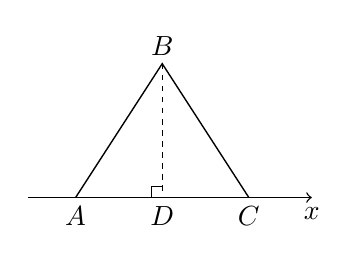
\begin{tikzpicture}[scale=1,line width=0.5pt]
\draw[->] (-0.4,0) -- (3.2,0) node[below] {$x$};
\draw (0.2,0) -- (1.3,1.7) -- (2.4,0);
\node at (0.2,-0.24) {$A$};
\node at (1.3,-0.24) {$D$};
\node at (2.4,-0.24) {$C$};
\node at (1.3,1.92) {$B$};
\draw[dash pattern=on 2pt off 2pt] (1.3,1.7) -- (1.3,0);
\draw (1.16,0) -- (1.16,0.14) -- (1.3,0.14);
\end{tikzpicture}
\end{center}
\step{$AB=AC=BC=\dfrac{2\sqrt3}3$，则 $x_2=x_1+AD=x_1+\dfrac{\sqrt3}3$，$x_3=x_1+\dfrac{2\sqrt3}3$，}
\step{存在 $x_1=-\dfrac{\sqrt3}3$，使得 $x_2=x_1+\dfrac{\sqrt3}3=0\in\Q$，且 $x_3=x_1+\dfrac{2\sqrt3}3=\dfrac{\sqrt3}3$ 为无理数，}
\step{即 $D(x_2)=1$，$D(x_3)=0$ 与图形一致，符合题意，}
\step{此时，$S_{\triangle ABC}=\dfrac12AC\cdot BD=\dfrac{\sqrt3}3$.}
\step{综上所述，存在这样的点 $A$、$B$、$C$，该正三角形的面积为 $\dfrac{\sqrt3}3$.}
\solend

\fi

\item 已知函数 $f(x)$ 满足：对 $\forall x\in R$，都有 $f(x+2025)\leqslant f(x)+2026$，
$f(x+2026)\geqslant f(x)+2027$，若 $f(1)=0$，则 $f(2)$ 的取值范围是\blankline[4.4em].

\ifanswer
\solbegin
\step{对 $\forall x\in R$，都有 $f(x+2025)\leqslant f(x)+2026$，$f(x+2026)\geqslant f(x)+2027$，}
\step{则 $f(x)+2027\leqslant f(x+2026)=f(x+1+2025)\leqslant f(x+1)+2026$，}
\step{即 $f(x)+1\leqslant f(x+1)$，所以 $f(2)\geqslant f(1)+1=1$；}
\step{$f(x)+2026\geqslant f(x+2025)=f(x+2024+1)\geqslant f(x+2024)+1$}
\step{$\geqslant\cdots\geqslant f(x+1)+2024$，所以 $f(x)+2\geqslant f(x+1)$，}
\step{所以 $f(2)\leqslant f(1)+2=2$；}
\step{即 $f(2)$ 的取值范围是 $[1,2]$.}
\solend

\fi

\end{enumerate}

\bigsec{二、选择题}

\begin{enumerate}
\setcounter{enumi}{12}

\item 若实数 $0<m<n<1$，而实数 $x>1$，则下列不等式正确的是\mbox{（\quad）}

\keepwithprev
A. $m^x<n^x$\qquad\qquad B. $x^m>x^n$\qquad\qquad C. $\log_xm>\log_xn$\qquad D. $\log_mx<\log_nx$

\ifanswer
\solbegin
\step{对于 $A$，函数 $f(t)=t^x$ 是以 $t$ 为变量，$x$ 为常量的幂函数，}
\step{由于 $x>1$，易得 $f(t)$ 在 $(0,+\infty)$ 上严格增，}
\step{$0<m<n<1$，$x>1$，可以得到 $m^x<n^x$，故 $A$ 正确；}
\step{对于 $B$，函数 $g(s)=x^s$，是以 $s$ 为变量，$x$ 为常量的指数函数，}
\step{由于 $x>1$，则 $g(s)$ 严格增，$0<m<n<1$，可以得到 $x^m<x^n$，故 $B$ 不正确；}
\step{对于 $C$，$\log_xm=\dfrac{\lg m}{\lg x}$，$\log_xn=\dfrac{\lg n}{\lg x}$，由于 $0<m<n<1$，则 $\lg m<\lg n<0$，}
\step{$x>1$，则 $\lg x>0$，则有 $\dfrac{\lg m}{\lg x}<\dfrac{\lg n}{\lg x}$，即 $\log_xm<\log_xn$，故 $C$ 不正确；}
\step{对于 $D$，由 $\log_mx-\log_nx=\dfrac{\lg x}{\lg m}-\dfrac{\lg x}{\lg n}=\dfrac{\lg x(\lg n-\lg m)}{\lg m\lg n}$，}
\step{因为实数 $0<m<n<1$，而实数 $x>1$，}
\step{所以 $\lg x>0$，$\lg m<\lg n<0$，则 $\dfrac{\lg x(\lg n-\lg m)}{\lg m\lg n}>0$，即 $\log_mx>\log_nx$，}
\step{故 $D$ 不正确.}
\step{故选 $A$.}
\solend

\fi

\item 已知 $x>1$，$y>1$，则 “$4^x>2^y$” 是 $\log_2x>\log_4(y-1)$ ”的\mbox{（\quad）}

\keepwithprev
A. 充分不必要条件\qquad\qquad B. 必要不充分条件

C. 充要条件\qquad\qquad D. 既不充分也不必要条件

\ifanswer
\solbegin
\step{因为 $x>1$，$y>1$，若 $4^x>2^y$，即 $2^{2x}>2^y$，所以 $2x>y>1$，}
\step{因为 $\dfrac y2-\sqrt{y-1}=\dfrac{(\sqrt{y-1})^2-2\sqrt{y-1}+1}2=\dfrac{(\sqrt{y-1}-1)^2}2\geqslant0$，}
\step{即 $\dfrac y2\geqslant\sqrt{y-1}>0$，所以 $\log_2\dfrac y2\geqslant\log_2\sqrt{y-1}=\dfrac12\log_2(y-1)=\log_4(y-1)$，}
\step{又 $x>\dfrac y2>\dfrac12$，所以 $\log_2x>\log_2\dfrac y2\geqslant\log_4(y-1)$，故充分性成立；}
\step{取 $x=2$，$y=4$，满足 $1=\log_2x>\log_4(y-1)=\log_43$，}
\step{但 $16=4^x=2^y=16$，即不满足 $4^x>2^y$，故必要性不成立.}% 链首链尾两个 16 系原卷笔误，应为 4^x=2^y=16，照录
\step{故选 $A$.}
\solend

\fi

\item 以下命题中，真命题的个数是\mbox{（\quad）}

①函数 $y=(x^2+1)^2+3$ 最小值为 3；②若 $2^a+\log_2a=4^b+2\log_4b$，则 $a<2b$；③不等式
$2^x-x-1>0$ 的解集为 $(1,+\infty)$.

\keepwithprev
A. $0$\qquad\qquad B. $1$\qquad\qquad C. $2$\qquad\qquad D. $3$

\ifanswer
\solbegin
\step{对于①，由于 $x^2+1\geqslant1$，则 $y=(x^2+1)^2+3\geqslant4$，}
\step{即函数 $y=(x^2+1)^2+3$ 最小值为 4，①错误；}
\step{对于②，由于 $b>0$，}
\step{则有 $2^a+\log_2a=4^b+2\log_4b=2^{2b}+\log_2b<2^{2b}+\log_22b$，}
\step{设 $f(x)=2^x+\log_2x$，易得 $f(x)$ 在 $(0,+\infty)$ 上为严格增函数，必有 $a<2b$，}
\step{②正确；}
\step{对于③，当 $x=-1$ 时，$2^x-x-1=2^x(x+1)>0$，即 $-1$ 在不等式的解集内，}
\step{③错误；}
\step{故选 $B$.}
\solend

\fi

\item 已知函数 $f(x)=ax^2+bx+c$（$a\neq0$ 且 $a<b$），若对任意的 $x\in R$，$f(x)\geqslant0$，且
$f(1)\geqslant\lambda(b-a)$，则实数 $\lambda$ 的取值范围为\mbox{（\quad）}

\keepwithprev
A. $(-\infty,2]$\qquad\qquad B. $[2\text{，}+\infty)$\qquad\qquad C. $(-\infty\text{，}3]$\qquad\qquad D. $[3\text{，}+\infty)$% 原卷 B/C/D 用全角逗号、A 用半角，照录

\ifanswer
\solbegin
\step{因为函数 $f(x)\geqslant0$ 恒成立，所以 $a>0$，且 $\Delta=b^2-4ac\leqslant0$，即 $c\geqslant\dfrac{b^2}{4a}$，}
\step{所以 $a+b+c\geqslant a+b+\dfrac{b^2}{4a}$，又 $a<b$，所以 $b-a>0$，}
\step{又 $f(1)\geqslant\lambda(b-a)$ 恒成立，所以 $a+b+c\geqslant\lambda(b-a)$ 恒成立，}
\step{即 $\lambda\leqslant\left(\dfrac{a+b+c}{b-a}\right)_{\min}=\dfrac{a+b+\dfrac{b^2}{4a}}{b-a}$，}
\step{令 $t=\dfrac ba$（$t>1$），则 $\dfrac{a+b+\dfrac{b^2}{4a}}{b-a}=\dfrac{1+t+\dfrac{t^2}4}{t-1}$，}
\step{令 $\mu=t-1$（$\mu>0$），则 $t=\mu+1$，}
\step{故上式 $=\dfrac{1+\mu+1+\dfrac{(\mu+1)^2}4}{\mu}=\dfrac14\left(\mu+\dfrac9\mu+6\right)$，}
\step{对 $\mu>0$，有 $\mu+\dfrac9\mu\geqslant2\sqrt{\mu\times\dfrac9\mu}=6$，当且仅当 $\mu=\dfrac9\mu$，即 $\mu=3$ 时取等号，}
\step{所以 $\dfrac14\left(\mu+\dfrac9\mu+6\right)\geqslant\dfrac14(6+6)=3$，故 $\lambda\leqslant3$，}
\step{即实数 $\lambda$ 的取值范围为 $(-\infty,3]$. 故选 $C$.}
\solend

\fi

\end{enumerate}

\bigsec{三、解答题}

\begin{enumerate}
\setcounter{enumi}{16}

\item 已知函数 $f(x)=\log_\frac23(ax^2-6x+18)$.

（1）若 $f(x)$ 的定义域为 $R$，求实数 $a$ 的取值范围.

（2）若 $f(x)$ 的值域为 $R$，求实数 $a$ 的取值范围.

\ansspace*[10]

\ifanswer
\solbegin
\stepm{（1）}{由 $f(x)=\log_\frac23(ax^2-6x+18)$ 的定义域为 $R$，得 $ax^2-6x+18>0$ 恒成立，}
\step{$a=0$ 时，$f(x)=\log_\frac23(18-6x)$ 的定义域为 $(-\infty,3)$，不符合题意.}
\step{$a\neq0$ 时，$\begin{cases}a>0\\ \Delta=36-4\times18a<0\end{cases}$，解得 $a>\dfrac12$.}
\step{综上，$a$ 的取值范围是 $\left(\dfrac12,+\infty\right)$.}
\stepm{（2）}{$a=0$ 时，$f(x)=\log_\frac23(18-6x)$ 的值域为 $R$，符合题意.}
\step{$a\neq0$ 时，$\begin{cases}a>0\\ \Delta=36-4\times18a\geqslant0\end{cases}$，解得 $0<a\leqslant\dfrac12$.}
\step{综上，$a$ 的取值范围是 $\left[0,\dfrac12\right]$.}
\solend

\fi

\item 已知 $f(x)=\log_ax+\log_a(6-x)$，$a>0$ 且 $a\neq1$，且 $f(3)=2$.

（1）求 $a$ 的值及 $f(x)$ 的单调区间.

（2）若对于 $\forall x_1\in(0,6)$，$\exists x_2\in[1,9]$，使得 $f(x_1)\leqslant t+\log_3x_2$ 成立，求实数 $t$ 的取值范
围.

\ansspace*[12]

\ifanswer
\solbegin
\stepm{（1）}{已知 $f(x)=\log_ax+\log_a(6-x)$，且 $f(3)=2$.}
\step{得 $\log_a3+\log_a(6-3)=2$，即 $2\log_a3=2$，}
\step{因此 $\log_a3=1$，因此 $a=3$，因此 $f(x)=\log_3x+\log_3(6-x)$，}
\step{因为 $\begin{cases}x>0\\ 6-x>0\end{cases}$，因此 $0<x<6$，故 $f(x)$ 的定义域为 $(0,6)$；}
\step{$f(x)=\log_3(6x-x^2)$，}
\step{因为函数 $y=6x-x^2$ 在 $(0,3)$ 上严格增，在 $(3,6)$ 上严格减，}
\step{又函数 $y=\log_3x$ 为严格增函数，}
\step{由复合函数的单调性得函数 $f(x)$ 在 $(0,3)$ 上严格增，在 $(3,6)$ 上严格减；}
\stepm{（2）}{令 $g(x)=t+\log_3x$，}
\step{因为 $\forall x_1\in(0,6)$，$\exists x_2\in[1,9]$，使得 $f(x_1)\leqslant t+\log_3x_2$，}
\step{即 $f(x_{1})_{\max}\leqslant g(x_{2})_{\max}$，}
\step{其中由（1）得 $f(x_{1})_{\max}=f(3)=2$.}
\step{又 $g(x)=t+\log_3x$ 在 $[1,9]$ 上严格增，因此 $g(x)_{\max}=g(9)=t+2$，}
\step{因此 $2\leqslant t+2$，因此实数 $t$ 的取值范围为 $[0,+\infty)$.}
\solend

\fi

\item 某心理学研究小组在对学生上课注意力集中情况的调查研究中，发现其注意力指数 $p$ 与
听课时间 $t$ 之间的关系满足如图所示的曲线. 当 $t\in(0,14]$ 时，曲线是二次函数图象的一部
分，当 $t\in[14,40]$ 时，曲线是函数 $y=\log_a(t-5)+83$（$a>0$ 且 $a\neq1$）图象的一部分. 根据
专家研究，当注意力指数 $p$ 大于等于 80 时听课效果最佳.

（1）试求 $p=f(t)$ 的函数关系式；

（2）当一位学生在坚持听课 32 分钟时，注意力指数 $p$ 大约为多少？

（3）一道数学难题，讲解需要 20 分钟，问老师能否经过合理安排在学生听
课效果最佳时讲完？请说明理由.

\begin{center}
% 原图第 9 页题干 p-t 曲线图按原图形状用 TikZ 重排（三版都出）。
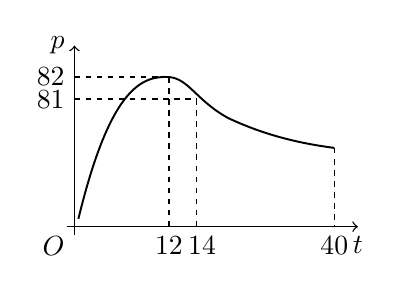
\begin{tikzpicture}[scale=1,line width=0.5pt]
\draw[->] (-0.1,0) -- (3.6,0) node[below] {$t$};
\draw[->] (0,-0.1) -- (0,2.3) node[left] {$p$};
\node[below left] at (0,0) {$O$};
\draw[line width=0.7pt] (0.05,0.1) .. controls (0.45,1.75) and (0.85,1.92) .. (1.2,1.9)
  .. controls (1.45,1.88) and (1.55,1.6) .. (1.95,1.38)
  .. controls (2.5,1.12) and (3.0,1.04) .. (3.3,1.0);
\draw[dash pattern=on 2pt off 2pt] (0,1.9) -- (1.2,1.9);
\draw[dash pattern=on 2pt off 2pt] (0,1.62) -- (1.55,1.62);
\draw[dash pattern=on 2pt off 2pt] (1.2,1.9) -- (1.2,0);
\draw[dash pattern=on 2pt off 2pt] (1.55,1.62) -- (1.55,0);
\draw[dash pattern=on 2pt off 2pt] (3.3,1.0) -- (3.3,0);
\node[left] at (0,1.9) {$82$};
\node[left] at (0,1.62) {$81$};
\node[below] at (1.2,0) {$12$};
\node[below] at (1.62,0) {$14$};
\node[below] at (3.3,0) {$40$};
\end{tikzpicture}
\end{center}

\ansspace*[12]

\ifanswer
\solbegin
\stepm{（1）}{由题意得当 $t\in(0,14]$ 时，设 $f(t)=c(t-12)^2+82$（$c<0$），}
\step{又 $f(14)=81$，所以 $c(14-12)^2+82=81$，解得 $c=-\dfrac14$；}
\step{所以 $f(t)=-\dfrac14(t-12)^2+82$,$t\in(0,14]$；}
\step{又当 $t\in[14,40]$ 时，函数 $y=\log_a(t-5)+83$（$a>0$ 且 $a\neq1$），}
\step{又当 $x=14$ 时，$y=81$，所以 $81=\log_a(14-5)+83$，解得 $a=\dfrac13$；}
\step{所以 $f(t)=\log_\frac13(t-5)+83$,$t\in[14,40]$，}
\step{所以 $p=\begin{cases}-\dfrac14(t-12)^2+82, & t\in(0,14]\\ \log_\frac13(t-5)+83, & t\in(14,40]\end{cases}$；}
\stepm{（2）}{当 $t=32$ 时，$p=\log_\frac13(32-5)+83=80$，}
\step{所以当一位学生在坚持听课 32 分钟时，注意力指数 $p$ 大约为 80；}
\stepm{（3）}{当 $t\in(0,14]$ 时，$-\dfrac14(t-12)^2+82\geqslant80$，解得 $t\in[12-2\sqrt2,14]$，}
\step{当 $t\in[14,40]$ 时，$\log_\frac13(t-5)+83\geqslant80$，解得 $5<t\leqslant32$，则 $t\in[14,32]$，}
\step{因此当 $t\in[12-2\sqrt2,32]$ 时学生听课效果最佳，}
\step{此时 $\Delta t=32-(12-2\sqrt2)=20+2\sqrt2>20$，}
\step{所以老师能经过合理安排时间在学生听课效果最佳时段讲完.}
\solend

\fi

\item 已知 $a\in R$，函数 $f(x+1)=\log_2\left(\dfrac{ax+1+a}{x+1}\right)$.

（1）若 $a=2$，求函数 $f(x)$ 的表达式及定义域；

（2）若关于 $x$ 的方程 $f\left(\dfrac x2\right)-\log_2[(a-2)x+3a-5]=0$ 的解集中恰好只有一个元素，求实
数 $a$ 的取值范围.

\ansspace*[14]

\ifanswer
\solbegin
\stepm{（1）}{$f(x+1)=\log_2\left(\dfrac{ax+1+a}{x+1}\right)$，}
\step{令 $x+1=t$，则 $f(t)=\log_2\left(\dfrac1t+a\right)$，即 $f(x)=\log_2\left(\dfrac1x+a\right)$，}
\step{因为 $a=2$，所以 $f(x)=\log_2\left(2+\dfrac1x\right)$，}
\step{由 $2+\dfrac1x>0$ 得定义域为 $\left(-\infty,-\dfrac12\right)\cup(0,+\infty)$；}
\stepm{（2）}{由（1）得 $f(x)=\log_2\left(\dfrac1x+a\right)$，}
\step{方程 $f\left(\dfrac x2\right)-\log_2[(a-2)x+3a-5]=0$，}
\step{即 $\log_2\left(\dfrac2x+a\right)-\log_2[(a-2)x+3a-5]=0$，}
\step{可转化为 $(a-2)x^2+(2a-5)x-2=0$，且 $\dfrac2x+a>0$.}
\step{①当 $a-2=0$，即 $a=2$ 时，$x=-2$，符合题意；}
\step{②当 $a-2\neq0$，即 $a\neq2$ 时，$x_1=-2$,$x_2=\dfrac1{a-2}$，}
\step{（$i$）当 $-2=\dfrac1{a-2}$ 时，即 $a=\dfrac32$ 时，符合题意；}
\step{（$ii$）当 $-2\neq\dfrac1{a-2}$ 时，即 $a\neq\dfrac32$ 且 $a\neq2$ 时，}
\step{要满足题意，则有 $\begin{cases}-1+a>0\\ 3a-4\leqslant0\end{cases}\Rightarrow1<a\leqslant\dfrac43$ 或 $\begin{cases}-1+a\leqslant0\\ 3a-4>0\end{cases}$，无解；}
\step{综上，$a$ 的取值范围 $\left(1,\dfrac43\right]\cup\left\{2,\dfrac32\right\}$.}
\solend

\fi

\item 已知函数 $y=f(x)$ 是定义在 $[0,+\infty)$ 上的函数，并且 $f(x)\geqslant0$，对于定义域内的任意自
变量的值 $x$、$y$，满足 $f(y)f(x^2f(y)+xf(y))=f(x^2+y+x)$，$f(a)=0$，其中
$a>0$.

（1）当 $f(0)\neq0$ 时，求 $f(0)$；

（2）已知当 $0\leqslant x<a$ 时，有 $f(x)\neq0$.

（$i$）求 $f(a+3)$；

（$ii$）求函数 $y=f(x)$ 的解析式（用 $a$ 表示）.

\ansspace*[16]

\ifanswer
\solbegin
\stepm{（1）}{因为 $f(x)\geqslant0$，且对于定义域内的任意自变量的值 $x$、$y$，}
\step{满足 $f(y)f(x^2f(y)+xf(y))=f(x^2+y+x)$，}
\step{令 $x=y=0$，则 $f^2(0)=f(0)$，因为 $f(0)\neq0$，所以 $f(0)=1$，}
\stepm{（2）}{（$i$）由 $f(y)f(x^2f(y)+xf(y))=f(x^2+y+x)$，}
\step{得 $f(y)f[(x^2+x)f(y)]=f[(x^2+x)+y]$，}
\step{令 $t=x^2+x$，因为 $x\geqslant0$，所以 $t=x^2+x\in[0,+\infty)$，}
\step{所以有 $f(y)f(tf(y))=f(t+y)$，因为 $f(a)=0$，}
\step{令 $y=a$，$t=3$，得 $f(a+3)=f(a)f(3f(a))=0\times f(3f(a))=0$；}
\step{（$ii$）当 $x\geqslant a$ 时，令 $y=a$，$t=x-a$，}
\step{$f(x)=f(x-a+a)=f(a)f[(x-a)f(a)]=0$.}
\step{当 $0\leqslant x<a$ 时，则有 $0<a-x\leqslant a$，令 $y=x$，$t=a-x$，}
\step{则 $f(a)=f(a-x+x)=f(x)f[(a-x)f(x)]=0$.}
\step{因为 $f(x)\neq0$，所以有 $f((a-x)f(x))=0$，则 $(a-x)f(x)\geqslant a$，}
\step{又因为 $a-x>0$，即 $f(x)\geqslant\dfrac a{a-x}$.}
\step{令 $t=\dfrac a{f(x)}>0$,$y=x>0$，}
\step{则 $f\left(\dfrac a{f(x)}+x\right)=f(x)\cdot f\left(\dfrac a{f(x)}\cdot f(x)\right)=f(x)\cdot f(a)=0$，}
\step{所以有 $\dfrac a{f(x)}+x\geqslant a$，即 $\dfrac a{f(x)}\geqslant a-x$，得 $f(x)\leqslant\dfrac a{a-x}$，}
\step{所以当 $0\leqslant x<a$ 时，$f(x)=\dfrac a{a-x}$.}
\step{综上，$f(x)=\begin{cases}\dfrac a{a-x}, & 0\leqslant x<a\\ 0, & x\geqslant a\end{cases}$.}
\solend

\fi

\end{enumerate}

\end{document}
"
% 紧凑版：xelatex "\def\iscompact{1}% 高一105_交附闵行_周末作业10.30.tex
%   —— 高一上数学“2026-2027 年交附闵行高一上周末作业 10.30”（试卷版/答案版）
% 试卷版：xelatex 高一105_交附闵行_周末作业10.30.tex
% 答案版：xelatex "\def\isanswer{1}\input{高一105_交附闵行_周末作业10.30.tex}"
% 紧凑版：xelatex "\def\iscompact{1}\input{高一105_交附闵行_周末作业10.30.tex}"
%
% 原始材料：微信公众号“魔都数学加油站”文章，作者破晓，2026-11-02 17:41 发布；
% 连载“27学年高一105”，原文标题“27学年高一105——2026-2027年上海市交附闵行高一上周末作业10.30”；
% 原文链接：https://mp.weixin.qq.com/s/XUfNEvGHjD0CB5jdoleBWw。
% 正文为 13 张 PNG 页（第 4、9、13 页 2560×3620，其余 4762×6735），题目下印有【解析】，为讲评版。
% 题目、解析均据原图转录；卷面水印及公众号页脚未录入。
%
% 卷首标题：原卷印作“2026-2027 年交附闵行高一上周末作业 10.30”（公众号标题中的“上海市”
% 卷面标题行没有，本稿照卷面），年份区间按全稿惯例排 en dash；原卷未印副标题，本稿按题目
% 内容标为“函数、不等式”（主体为指数与对数，第 3 题集合、第 16 题基本不等式）。
%
% 与原卷的排版差异：
%   ① 原文从第 3 题起，填空题编号为 3—12、选择题为 13—16、解答题为 17—21，本稿保留原题号；
%   ② 原卷每题下直接印【解析】，本稿按全稿惯例将解析置于答案版；选择题括号内未印答案，另由
%      解析末句“故选 X”给出；
%   ③ 原卷未印副标题，本稿按“知识模块”口径补出；
%   ④ 原卷填空横线按全稿惯例排为 \blankline[4.4em]；解答题按惯例加 \ansspace；选择题括号排
%      \mbox{（\quad）}、选项段前按惯例加 \keepwithprev；
%   ⑤ $f(x_1)_{max}$、$g(x)_max$、$\left(\frac{a+b+c}{b-a}\right)_{min}$ 等下标原卷排斜体，
%      按 高一96 成例改正体 $\max$、$\min$；
%   ⑥ 原卷数集排斜体 $R$／$Q$，按全稿惯例改 $\R$／$\Q$；
%   ⑦ 第 11 题解析的两幅三角形示意图与第 19 题题干的 $p$-$t$ 曲线图均按原图形状用 TikZ 重排
%      （第 19 题图属题干、三版都出；第 11 题图属解析、仅答案版显示）。
%
% 原卷存疑／笔误（均照录加注）：
%   第 14 题解析“但 $16=4^x=2^y=16$”（链首、链尾的两个 $16$ 系原卷笔误，按上下文应为
%   $4^x=2^y=16$）；
%   第 16 题选项的区间分隔逗号 A 项排半角、B／C／D 三项排全角（原卷自身不一致）；
%   第 21 题 (2) 的小问号排“（$i$）求…”（右括号紧贴“求”字），照录。
%
% 行数核对：逐题数 \step/\stepm 条数，合计 159 条（Q3：2；Q4：1；Q5：4；Q6：6；Q7：3；
% Q8：7；Q9：5；Q10：3；Q11：15；Q12：7；Q13：12；Q14：7；Q15：9；Q16：10；Q17：7；
% Q18：14；Q19：14；Q20：14；Q21：19），与原卷印刷行逐题相等。
%
\documentclass[a4paper,11pt]{article}
\usepackage{common}

\begin{document}

\examtitlest[3]{2026--2027 年交附闵行高一上周末作业 10.30}{函数、不等式}

\bigsec{一、填空题}

\begin{enumerate}
\setcounter{enumi}{2}

\item 已知集合 $M=\{1,m\}$，$N=\{n,\log_2n\}$，若 $M=N$，则 $(m-n)^{2027}=$\blankline[4.4em].

\ifanswer
\solbegin
\step{由题意得 $\begin{cases}n=1\\ \log_2n=m\end{cases}$ 或 $\begin{cases}n=m\\ \log_2n=1\end{cases}$，解得 $\begin{cases}n=1\\ m=0\end{cases}$ 或 $\begin{cases}n=2\\ m=2\end{cases}$，}
\step{所以 $(m-n)^{2027}=-1$ 或 $0$.}
\solend

\fi

\item 已知 $\log_{2x^2-1}(3x^2+2x-1)=1$，则 $x=$\blankline[4.4em].

\ifanswer
\solbegin
\step{因为 $\log_{2x^2-1}(3x^2+2x-1)=1$，所以 $\begin{cases}2x^2-1>0\\ 2x^2-1\neq1\\ 3x^2+2x-1>0\\ 2x^2-1=3x^2+2x-1\end{cases}$，解得 $x=-2$.}
\solend

\fi

\item 已知 $m>1$，$n>1$，$\lg m=\log_n100$，则 $mn$ 的最小值为\blankline[4.4em].

\ifanswer
\solbegin
\step{由 $m>1$，$n>1$，得 $\lg m>0$，$\lg n>0$，}
\step{因为 $\lg m=\log_n100=\dfrac{\lg100}{\lg n}=\dfrac2{\lg n}$，所以 $\lg m\cdot\lg n=2$，}
\step{所以 $\lg(mn)=\lg m+\lg n\geqslant2\sqrt{\lg m\cdot\lg n}=2\sqrt2$，}
\step{当且仅当 $m=n=10^{\sqrt2}$ 时取等号，则 $mn\geqslant10^{2\sqrt2}$，即 $mn$ 的最小值为 $10^{2\sqrt2}$.}
\solend

\fi

\item 设 $m$、$n$ 分别是方程 $\log_{2013}x+x-9=0$ 和 $2013^x+x-9=0$ 的根，则 $m+n=$\blankline[4.4em].

\ifanswer
\solbegin
\step{由 $\log_{2013}x+x-9=0$，得 $\log_{2013}x=-x+9$，}
\step{因为 $m$ 是方程 $\log_{2013}x+x-9=0$ 的根，}
\step{所以 $m$ 为函数 $y=\log_{2013}x$ 与 $y=-x+9$ 图象交点的横坐标，}
\step{同理 $n$ 是函数 $y=2013^x$ 与 $y=-x+9$ 图象交点的横坐标，}
\step{因为 $y=\log_{2013}x$ 与 $y=2013^x$ 互为反函数，其图象关于直线 $y=x$ 对称，}
\step{联立 $\begin{cases}y=-x+9\\ y=x\end{cases}$，解得 $x=\dfrac92$，所以 $m+n=\dfrac92\times2=9$.}
\solend

\fi

\item 已知函数 $f(x)=\dfrac1{\log_2(x^2+4)}$，则 $f(-2)=$\blankline[2em]，$f(x)$ 的值域为\blankline[4.4em].

\ifanswer
\solbegin
\step{$f(-2)=\dfrac1{\log_28}=\dfrac13$.}
\step{因为 $x^2+4\geqslant4$，所以 $\log_2(x^2+4)\geqslant\log_24=2$，所以 $0<\dfrac1{\log_2(x^2+4)}\leqslant\dfrac12$，}
\step{故 $f(x)$ 的值域为 $\left(0,\dfrac12\right]$.}
\solend

\fi

\item 已知 $\alpha$、$\beta$ 是方程 $9^x-2m\cdot3^x+m^2-1=0$ 的两个根，若 $\alpha+\beta=1$，则 $\alpha\beta=$\blankline[4.4em].

\ifanswer
\solbegin
\step{由题意得方程 $9^x-2m\cdot3^x+m^2-1=0$ 有两个根，}
\step{则方程 $t^2-2mt+m^2-1=0$ 有二正根，}
\step{则 $\begin{cases}\Delta=4m^2-4(m^2-1)\geqslant0\\ 2m>0\\ m^2-1>0\end{cases}$，解得 $m>1$，}
\step{又 $\alpha$、$\beta$ 是方程 $9^x-2m\cdot3^x+m^2-1=0$ 的两个根，}
\step{则 $3^\alpha\times3^\beta=m^2-1$，又 $\alpha+\beta=1$，则 $m^2-1=3^{\alpha+\beta}=3$，}
\step{解得 $m=2$ 或 $m=-2$（舍），则 $3^\alpha+3^\beta=2m=4$，又 $\alpha=1-\beta$，}
\step{则 $3^{1-\beta}+3^\beta=4$，解得 $\beta=0$ 或 $\beta=1$，则 $\begin{cases}\alpha=1\\ \beta=0\end{cases}$ 或 $\begin{cases}\alpha=0\\ \beta=1\end{cases}$，则 $\alpha\beta=0$.}
\solend

\fi

\item 已知 $a>b>0$，$\ln a=2\ln b$，且 $a\lg b=b\lg a$，则 $a+b=$\blankline[4.4em].

\ifanswer
\solbegin
\step{因为 $a>b>0$，$\ln a=2\ln b=\ln b^2$，所以 $a=b^2$，}
\step{由 $a\lg b=b\lg a$ 得 $b^2\lg b=b\lg b^2$，即 $b\lg b=2\lg b$，所以 $b=1$ 或 $b=2$，}
\step{当 $b=2$，$a=4$，满足题意，}
\step{当 $b=1$ 时，$a=1$ 与 $a>b>0$ 矛盾，所以 $b=1$ 舍去，}
\step{所以 $a+b=6$.}
\solend

\fi

\item 函数 $f(x)=\begin{cases}2^x, & x\leqslant t\\ \log_\frac12x, & x>t\end{cases}$ 的值域为 $M$，且 $8\notin M$，则实数 $t$ 的取值集合为\blankline[4.4em].

\ifanswer
\solbegin
\step{当 $x\leqslant t$ 时，函数 $f(x)=2^x$ 在 $(-\infty,t]$ 严格增，}
\step{当 $x>t$ 时，$f(x)=\log_\frac12x$ 在 $(t,+\infty)$ 严格减，}
\step{若 $8\notin M$，则满足条件 $\begin{cases}2^t<8\\ \log_\frac12t\leqslant8\end{cases}\Rightarrow\dfrac1{256}\leqslant t<3$，故实数 $t$ 的取值集合为 $\left[\dfrac1{256},3\right)$.}
\solend

\fi

\item 德国数学家狄利克雷在数学领域成就显著，以其命名函数 $D(x)=\begin{cases}1, & x\text{为有理数}\\ 0, & x\text{为无理数}\end{cases}$，该函
数被称为狄利克雷函数。那么是否存在三个点 $A(x_1,D(x_1))$、$B(x_2,D(x_2))$、$C(x_3,D(x_3))$，
使得 $\triangle ABC$ 为等边三角形，若不存在请在横线上填写“不存在”，如果存在则在横线上填写
该正三角形的面积\blankline[4.4em].

\ifanswer
\solbegin
\step{因为 $D(x)=\begin{cases}1, & x\text{为有理数}\\ 0, & x\text{为无理数}\end{cases}$，所以 $D(x)=0$ 或 1，}
\step{设存在三个点 $A(x_1,D(x_1))$、$B(x_2,D(x_2))$、$C(x_3,D(x_3))$，}
\step{使得 $\triangle ABC$ 为等边三角形，则 $D(x_1)$、$D(x_2)$、$D(x_3)$ 不同时为 0 或 1，}
\step{不妨设 $x_1<x_2<x_3$，分析得 $\triangle ABC$ 的位置有两种情况，}
\step{第一种情况：当 $x_1$ 为有理数时，即 $D(x_1)=1$，如图，过点 $B$ 作 $BD\perp AC$，}
\begin{center}
% 原图第 4 页解析示意图按原图形状用 TikZ 重排（第一种情况：$B$ 在 $x$ 轴上、$AC$ 在上方）。
\begin{tikzpicture}[scale=1,line width=0.5pt]
\draw (0,1.2) -- (2.6,1.2);
\node at (0.25,1.4) {$A$};
\node at (1.3,1.4) {$D$};
\node at (2.35,1.4) {$C$};
\draw[dash pattern=on 2pt off 2pt] (1.3,1.2) -- (1.3,0);
\draw (1.16,1.2) -- (1.16,1.06) -- (1.3,1.06);
\draw[->] (-0.5,0) -- (3.1,0) node[below] {$x$};
\node at (1.3,-0.24) {$B$};
\end{tikzpicture}
\end{center}
\step{垂足为 $D$，得 $BD=1$，$AD=\dfrac{\sqrt3}3$，$AB=AC=BC=\dfrac{2\sqrt3}3$，}
\step{则 $x_2=x_1+AD=x_1+\dfrac{\sqrt3}3$ 为无理数，$x_3=x_1+\dfrac{2\sqrt3}3$ 为无理数，}
\step{即 $D(x_2)=0$，$D(x_3)=0$ 与图形不一致，舍去；}
\step{第二种情况：当 $x_1$ 为无理数时，即 $D(x_1)=0$，如图，}
\step{过点 $B$ 作 $BD\perp AC$，垂足为 $D$，得 $BD=1$，$AD=\dfrac{\sqrt3}3$，}
\begin{center}
% 原图第 4 页解析示意图按原图形状用 TikZ 重排（第二种情况：$B$ 在上方、$AC$ 在 $x$ 轴上）。
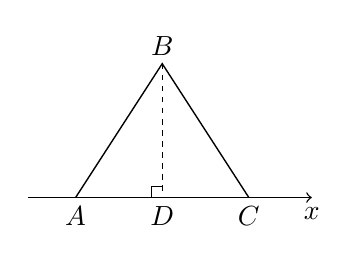
\begin{tikzpicture}[scale=1,line width=0.5pt]
\draw[->] (-0.4,0) -- (3.2,0) node[below] {$x$};
\draw (0.2,0) -- (1.3,1.7) -- (2.4,0);
\node at (0.2,-0.24) {$A$};
\node at (1.3,-0.24) {$D$};
\node at (2.4,-0.24) {$C$};
\node at (1.3,1.92) {$B$};
\draw[dash pattern=on 2pt off 2pt] (1.3,1.7) -- (1.3,0);
\draw (1.16,0) -- (1.16,0.14) -- (1.3,0.14);
\end{tikzpicture}
\end{center}
\step{$AB=AC=BC=\dfrac{2\sqrt3}3$，则 $x_2=x_1+AD=x_1+\dfrac{\sqrt3}3$，$x_3=x_1+\dfrac{2\sqrt3}3$，}
\step{存在 $x_1=-\dfrac{\sqrt3}3$，使得 $x_2=x_1+\dfrac{\sqrt3}3=0\in\Q$，且 $x_3=x_1+\dfrac{2\sqrt3}3=\dfrac{\sqrt3}3$ 为无理数，}
\step{即 $D(x_2)=1$，$D(x_3)=0$ 与图形一致，符合题意，}
\step{此时，$S_{\triangle ABC}=\dfrac12AC\cdot BD=\dfrac{\sqrt3}3$.}
\step{综上所述，存在这样的点 $A$、$B$、$C$，该正三角形的面积为 $\dfrac{\sqrt3}3$.}
\solend

\fi

\item 已知函数 $f(x)$ 满足：对 $\forall x\in R$，都有 $f(x+2025)\leqslant f(x)+2026$，
$f(x+2026)\geqslant f(x)+2027$，若 $f(1)=0$，则 $f(2)$ 的取值范围是\blankline[4.4em].

\ifanswer
\solbegin
\step{对 $\forall x\in R$，都有 $f(x+2025)\leqslant f(x)+2026$，$f(x+2026)\geqslant f(x)+2027$，}
\step{则 $f(x)+2027\leqslant f(x+2026)=f(x+1+2025)\leqslant f(x+1)+2026$，}
\step{即 $f(x)+1\leqslant f(x+1)$，所以 $f(2)\geqslant f(1)+1=1$；}
\step{$f(x)+2026\geqslant f(x+2025)=f(x+2024+1)\geqslant f(x+2024)+1$}
\step{$\geqslant\cdots\geqslant f(x+1)+2024$，所以 $f(x)+2\geqslant f(x+1)$，}
\step{所以 $f(2)\leqslant f(1)+2=2$；}
\step{即 $f(2)$ 的取值范围是 $[1,2]$.}
\solend

\fi

\end{enumerate}

\bigsec{二、选择题}

\begin{enumerate}
\setcounter{enumi}{12}

\item 若实数 $0<m<n<1$，而实数 $x>1$，则下列不等式正确的是\mbox{（\quad）}

\keepwithprev
A. $m^x<n^x$\qquad\qquad B. $x^m>x^n$\qquad\qquad C. $\log_xm>\log_xn$\qquad D. $\log_mx<\log_nx$

\ifanswer
\solbegin
\step{对于 $A$，函数 $f(t)=t^x$ 是以 $t$ 为变量，$x$ 为常量的幂函数，}
\step{由于 $x>1$，易得 $f(t)$ 在 $(0,+\infty)$ 上严格增，}
\step{$0<m<n<1$，$x>1$，可以得到 $m^x<n^x$，故 $A$ 正确；}
\step{对于 $B$，函数 $g(s)=x^s$，是以 $s$ 为变量，$x$ 为常量的指数函数，}
\step{由于 $x>1$，则 $g(s)$ 严格增，$0<m<n<1$，可以得到 $x^m<x^n$，故 $B$ 不正确；}
\step{对于 $C$，$\log_xm=\dfrac{\lg m}{\lg x}$，$\log_xn=\dfrac{\lg n}{\lg x}$，由于 $0<m<n<1$，则 $\lg m<\lg n<0$，}
\step{$x>1$，则 $\lg x>0$，则有 $\dfrac{\lg m}{\lg x}<\dfrac{\lg n}{\lg x}$，即 $\log_xm<\log_xn$，故 $C$ 不正确；}
\step{对于 $D$，由 $\log_mx-\log_nx=\dfrac{\lg x}{\lg m}-\dfrac{\lg x}{\lg n}=\dfrac{\lg x(\lg n-\lg m)}{\lg m\lg n}$，}
\step{因为实数 $0<m<n<1$，而实数 $x>1$，}
\step{所以 $\lg x>0$，$\lg m<\lg n<0$，则 $\dfrac{\lg x(\lg n-\lg m)}{\lg m\lg n}>0$，即 $\log_mx>\log_nx$，}
\step{故 $D$ 不正确.}
\step{故选 $A$.}
\solend

\fi

\item 已知 $x>1$，$y>1$，则 “$4^x>2^y$” 是 $\log_2x>\log_4(y-1)$ ”的\mbox{（\quad）}

\keepwithprev
A. 充分不必要条件\qquad\qquad B. 必要不充分条件

C. 充要条件\qquad\qquad D. 既不充分也不必要条件

\ifanswer
\solbegin
\step{因为 $x>1$，$y>1$，若 $4^x>2^y$，即 $2^{2x}>2^y$，所以 $2x>y>1$，}
\step{因为 $\dfrac y2-\sqrt{y-1}=\dfrac{(\sqrt{y-1})^2-2\sqrt{y-1}+1}2=\dfrac{(\sqrt{y-1}-1)^2}2\geqslant0$，}
\step{即 $\dfrac y2\geqslant\sqrt{y-1}>0$，所以 $\log_2\dfrac y2\geqslant\log_2\sqrt{y-1}=\dfrac12\log_2(y-1)=\log_4(y-1)$，}
\step{又 $x>\dfrac y2>\dfrac12$，所以 $\log_2x>\log_2\dfrac y2\geqslant\log_4(y-1)$，故充分性成立；}
\step{取 $x=2$，$y=4$，满足 $1=\log_2x>\log_4(y-1)=\log_43$，}
\step{但 $16=4^x=2^y=16$，即不满足 $4^x>2^y$，故必要性不成立.}% 链首链尾两个 16 系原卷笔误，应为 4^x=2^y=16，照录
\step{故选 $A$.}
\solend

\fi

\item 以下命题中，真命题的个数是\mbox{（\quad）}

①函数 $y=(x^2+1)^2+3$ 最小值为 3；②若 $2^a+\log_2a=4^b+2\log_4b$，则 $a<2b$；③不等式
$2^x-x-1>0$ 的解集为 $(1,+\infty)$.

\keepwithprev
A. $0$\qquad\qquad B. $1$\qquad\qquad C. $2$\qquad\qquad D. $3$

\ifanswer
\solbegin
\step{对于①，由于 $x^2+1\geqslant1$，则 $y=(x^2+1)^2+3\geqslant4$，}
\step{即函数 $y=(x^2+1)^2+3$ 最小值为 4，①错误；}
\step{对于②，由于 $b>0$，}
\step{则有 $2^a+\log_2a=4^b+2\log_4b=2^{2b}+\log_2b<2^{2b}+\log_22b$，}
\step{设 $f(x)=2^x+\log_2x$，易得 $f(x)$ 在 $(0,+\infty)$ 上为严格增函数，必有 $a<2b$，}
\step{②正确；}
\step{对于③，当 $x=-1$ 时，$2^x-x-1=2^x(x+1)>0$，即 $-1$ 在不等式的解集内，}
\step{③错误；}
\step{故选 $B$.}
\solend

\fi

\item 已知函数 $f(x)=ax^2+bx+c$（$a\neq0$ 且 $a<b$），若对任意的 $x\in R$，$f(x)\geqslant0$，且
$f(1)\geqslant\lambda(b-a)$，则实数 $\lambda$ 的取值范围为\mbox{（\quad）}

\keepwithprev
A. $(-\infty,2]$\qquad\qquad B. $[2\text{，}+\infty)$\qquad\qquad C. $(-\infty\text{，}3]$\qquad\qquad D. $[3\text{，}+\infty)$% 原卷 B/C/D 用全角逗号、A 用半角，照录

\ifanswer
\solbegin
\step{因为函数 $f(x)\geqslant0$ 恒成立，所以 $a>0$，且 $\Delta=b^2-4ac\leqslant0$，即 $c\geqslant\dfrac{b^2}{4a}$，}
\step{所以 $a+b+c\geqslant a+b+\dfrac{b^2}{4a}$，又 $a<b$，所以 $b-a>0$，}
\step{又 $f(1)\geqslant\lambda(b-a)$ 恒成立，所以 $a+b+c\geqslant\lambda(b-a)$ 恒成立，}
\step{即 $\lambda\leqslant\left(\dfrac{a+b+c}{b-a}\right)_{\min}=\dfrac{a+b+\dfrac{b^2}{4a}}{b-a}$，}
\step{令 $t=\dfrac ba$（$t>1$），则 $\dfrac{a+b+\dfrac{b^2}{4a}}{b-a}=\dfrac{1+t+\dfrac{t^2}4}{t-1}$，}
\step{令 $\mu=t-1$（$\mu>0$），则 $t=\mu+1$，}
\step{故上式 $=\dfrac{1+\mu+1+\dfrac{(\mu+1)^2}4}{\mu}=\dfrac14\left(\mu+\dfrac9\mu+6\right)$，}
\step{对 $\mu>0$，有 $\mu+\dfrac9\mu\geqslant2\sqrt{\mu\times\dfrac9\mu}=6$，当且仅当 $\mu=\dfrac9\mu$，即 $\mu=3$ 时取等号，}
\step{所以 $\dfrac14\left(\mu+\dfrac9\mu+6\right)\geqslant\dfrac14(6+6)=3$，故 $\lambda\leqslant3$，}
\step{即实数 $\lambda$ 的取值范围为 $(-\infty,3]$. 故选 $C$.}
\solend

\fi

\end{enumerate}

\bigsec{三、解答题}

\begin{enumerate}
\setcounter{enumi}{16}

\item 已知函数 $f(x)=\log_\frac23(ax^2-6x+18)$.

（1）若 $f(x)$ 的定义域为 $R$，求实数 $a$ 的取值范围.

（2）若 $f(x)$ 的值域为 $R$，求实数 $a$ 的取值范围.

\ansspace*[10]

\ifanswer
\solbegin
\stepm{（1）}{由 $f(x)=\log_\frac23(ax^2-6x+18)$ 的定义域为 $R$，得 $ax^2-6x+18>0$ 恒成立，}
\step{$a=0$ 时，$f(x)=\log_\frac23(18-6x)$ 的定义域为 $(-\infty,3)$，不符合题意.}
\step{$a\neq0$ 时，$\begin{cases}a>0\\ \Delta=36-4\times18a<0\end{cases}$，解得 $a>\dfrac12$.}
\step{综上，$a$ 的取值范围是 $\left(\dfrac12,+\infty\right)$.}
\stepm{（2）}{$a=0$ 时，$f(x)=\log_\frac23(18-6x)$ 的值域为 $R$，符合题意.}
\step{$a\neq0$ 时，$\begin{cases}a>0\\ \Delta=36-4\times18a\geqslant0\end{cases}$，解得 $0<a\leqslant\dfrac12$.}
\step{综上，$a$ 的取值范围是 $\left[0,\dfrac12\right]$.}
\solend

\fi

\item 已知 $f(x)=\log_ax+\log_a(6-x)$，$a>0$ 且 $a\neq1$，且 $f(3)=2$.

（1）求 $a$ 的值及 $f(x)$ 的单调区间.

（2）若对于 $\forall x_1\in(0,6)$，$\exists x_2\in[1,9]$，使得 $f(x_1)\leqslant t+\log_3x_2$ 成立，求实数 $t$ 的取值范
围.

\ansspace*[12]

\ifanswer
\solbegin
\stepm{（1）}{已知 $f(x)=\log_ax+\log_a(6-x)$，且 $f(3)=2$.}
\step{得 $\log_a3+\log_a(6-3)=2$，即 $2\log_a3=2$，}
\step{因此 $\log_a3=1$，因此 $a=3$，因此 $f(x)=\log_3x+\log_3(6-x)$，}
\step{因为 $\begin{cases}x>0\\ 6-x>0\end{cases}$，因此 $0<x<6$，故 $f(x)$ 的定义域为 $(0,6)$；}
\step{$f(x)=\log_3(6x-x^2)$，}
\step{因为函数 $y=6x-x^2$ 在 $(0,3)$ 上严格增，在 $(3,6)$ 上严格减，}
\step{又函数 $y=\log_3x$ 为严格增函数，}
\step{由复合函数的单调性得函数 $f(x)$ 在 $(0,3)$ 上严格增，在 $(3,6)$ 上严格减；}
\stepm{（2）}{令 $g(x)=t+\log_3x$，}
\step{因为 $\forall x_1\in(0,6)$，$\exists x_2\in[1,9]$，使得 $f(x_1)\leqslant t+\log_3x_2$，}
\step{即 $f(x_{1})_{\max}\leqslant g(x_{2})_{\max}$，}
\step{其中由（1）得 $f(x_{1})_{\max}=f(3)=2$.}
\step{又 $g(x)=t+\log_3x$ 在 $[1,9]$ 上严格增，因此 $g(x)_{\max}=g(9)=t+2$，}
\step{因此 $2\leqslant t+2$，因此实数 $t$ 的取值范围为 $[0,+\infty)$.}
\solend

\fi

\item 某心理学研究小组在对学生上课注意力集中情况的调查研究中，发现其注意力指数 $p$ 与
听课时间 $t$ 之间的关系满足如图所示的曲线. 当 $t\in(0,14]$ 时，曲线是二次函数图象的一部
分，当 $t\in[14,40]$ 时，曲线是函数 $y=\log_a(t-5)+83$（$a>0$ 且 $a\neq1$）图象的一部分. 根据
专家研究，当注意力指数 $p$ 大于等于 80 时听课效果最佳.

（1）试求 $p=f(t)$ 的函数关系式；

（2）当一位学生在坚持听课 32 分钟时，注意力指数 $p$ 大约为多少？

（3）一道数学难题，讲解需要 20 分钟，问老师能否经过合理安排在学生听
课效果最佳时讲完？请说明理由.

\begin{center}
% 原图第 9 页题干 p-t 曲线图按原图形状用 TikZ 重排（三版都出）。
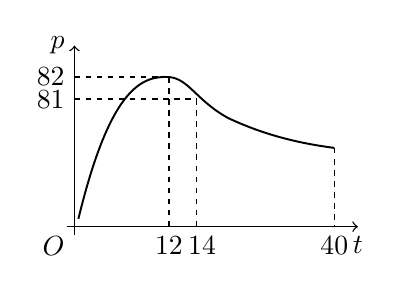
\begin{tikzpicture}[scale=1,line width=0.5pt]
\draw[->] (-0.1,0) -- (3.6,0) node[below] {$t$};
\draw[->] (0,-0.1) -- (0,2.3) node[left] {$p$};
\node[below left] at (0,0) {$O$};
\draw[line width=0.7pt] (0.05,0.1) .. controls (0.45,1.75) and (0.85,1.92) .. (1.2,1.9)
  .. controls (1.45,1.88) and (1.55,1.6) .. (1.95,1.38)
  .. controls (2.5,1.12) and (3.0,1.04) .. (3.3,1.0);
\draw[dash pattern=on 2pt off 2pt] (0,1.9) -- (1.2,1.9);
\draw[dash pattern=on 2pt off 2pt] (0,1.62) -- (1.55,1.62);
\draw[dash pattern=on 2pt off 2pt] (1.2,1.9) -- (1.2,0);
\draw[dash pattern=on 2pt off 2pt] (1.55,1.62) -- (1.55,0);
\draw[dash pattern=on 2pt off 2pt] (3.3,1.0) -- (3.3,0);
\node[left] at (0,1.9) {$82$};
\node[left] at (0,1.62) {$81$};
\node[below] at (1.2,0) {$12$};
\node[below] at (1.62,0) {$14$};
\node[below] at (3.3,0) {$40$};
\end{tikzpicture}
\end{center}

\ansspace*[12]

\ifanswer
\solbegin
\stepm{（1）}{由题意得当 $t\in(0,14]$ 时，设 $f(t)=c(t-12)^2+82$（$c<0$），}
\step{又 $f(14)=81$，所以 $c(14-12)^2+82=81$，解得 $c=-\dfrac14$；}
\step{所以 $f(t)=-\dfrac14(t-12)^2+82$,$t\in(0,14]$；}
\step{又当 $t\in[14,40]$ 时，函数 $y=\log_a(t-5)+83$（$a>0$ 且 $a\neq1$），}
\step{又当 $x=14$ 时，$y=81$，所以 $81=\log_a(14-5)+83$，解得 $a=\dfrac13$；}
\step{所以 $f(t)=\log_\frac13(t-5)+83$,$t\in[14,40]$，}
\step{所以 $p=\begin{cases}-\dfrac14(t-12)^2+82, & t\in(0,14]\\ \log_\frac13(t-5)+83, & t\in(14,40]\end{cases}$；}
\stepm{（2）}{当 $t=32$ 时，$p=\log_\frac13(32-5)+83=80$，}
\step{所以当一位学生在坚持听课 32 分钟时，注意力指数 $p$ 大约为 80；}
\stepm{（3）}{当 $t\in(0,14]$ 时，$-\dfrac14(t-12)^2+82\geqslant80$，解得 $t\in[12-2\sqrt2,14]$，}
\step{当 $t\in[14,40]$ 时，$\log_\frac13(t-5)+83\geqslant80$，解得 $5<t\leqslant32$，则 $t\in[14,32]$，}
\step{因此当 $t\in[12-2\sqrt2,32]$ 时学生听课效果最佳，}
\step{此时 $\Delta t=32-(12-2\sqrt2)=20+2\sqrt2>20$，}
\step{所以老师能经过合理安排时间在学生听课效果最佳时段讲完.}
\solend

\fi

\item 已知 $a\in R$，函数 $f(x+1)=\log_2\left(\dfrac{ax+1+a}{x+1}\right)$.

（1）若 $a=2$，求函数 $f(x)$ 的表达式及定义域；

（2）若关于 $x$ 的方程 $f\left(\dfrac x2\right)-\log_2[(a-2)x+3a-5]=0$ 的解集中恰好只有一个元素，求实
数 $a$ 的取值范围.

\ansspace*[14]

\ifanswer
\solbegin
\stepm{（1）}{$f(x+1)=\log_2\left(\dfrac{ax+1+a}{x+1}\right)$，}
\step{令 $x+1=t$，则 $f(t)=\log_2\left(\dfrac1t+a\right)$，即 $f(x)=\log_2\left(\dfrac1x+a\right)$，}
\step{因为 $a=2$，所以 $f(x)=\log_2\left(2+\dfrac1x\right)$，}
\step{由 $2+\dfrac1x>0$ 得定义域为 $\left(-\infty,-\dfrac12\right)\cup(0,+\infty)$；}
\stepm{（2）}{由（1）得 $f(x)=\log_2\left(\dfrac1x+a\right)$，}
\step{方程 $f\left(\dfrac x2\right)-\log_2[(a-2)x+3a-5]=0$，}
\step{即 $\log_2\left(\dfrac2x+a\right)-\log_2[(a-2)x+3a-5]=0$，}
\step{可转化为 $(a-2)x^2+(2a-5)x-2=0$，且 $\dfrac2x+a>0$.}
\step{①当 $a-2=0$，即 $a=2$ 时，$x=-2$，符合题意；}
\step{②当 $a-2\neq0$，即 $a\neq2$ 时，$x_1=-2$,$x_2=\dfrac1{a-2}$，}
\step{（$i$）当 $-2=\dfrac1{a-2}$ 时，即 $a=\dfrac32$ 时，符合题意；}
\step{（$ii$）当 $-2\neq\dfrac1{a-2}$ 时，即 $a\neq\dfrac32$ 且 $a\neq2$ 时，}
\step{要满足题意，则有 $\begin{cases}-1+a>0\\ 3a-4\leqslant0\end{cases}\Rightarrow1<a\leqslant\dfrac43$ 或 $\begin{cases}-1+a\leqslant0\\ 3a-4>0\end{cases}$，无解；}
\step{综上，$a$ 的取值范围 $\left(1,\dfrac43\right]\cup\left\{2,\dfrac32\right\}$.}
\solend

\fi

\item 已知函数 $y=f(x)$ 是定义在 $[0,+\infty)$ 上的函数，并且 $f(x)\geqslant0$，对于定义域内的任意自
变量的值 $x$、$y$，满足 $f(y)f(x^2f(y)+xf(y))=f(x^2+y+x)$，$f(a)=0$，其中
$a>0$.

（1）当 $f(0)\neq0$ 时，求 $f(0)$；

（2）已知当 $0\leqslant x<a$ 时，有 $f(x)\neq0$.

（$i$）求 $f(a+3)$；

（$ii$）求函数 $y=f(x)$ 的解析式（用 $a$ 表示）.

\ansspace*[16]

\ifanswer
\solbegin
\stepm{（1）}{因为 $f(x)\geqslant0$，且对于定义域内的任意自变量的值 $x$、$y$，}
\step{满足 $f(y)f(x^2f(y)+xf(y))=f(x^2+y+x)$，}
\step{令 $x=y=0$，则 $f^2(0)=f(0)$，因为 $f(0)\neq0$，所以 $f(0)=1$，}
\stepm{（2）}{（$i$）由 $f(y)f(x^2f(y)+xf(y))=f(x^2+y+x)$，}
\step{得 $f(y)f[(x^2+x)f(y)]=f[(x^2+x)+y]$，}
\step{令 $t=x^2+x$，因为 $x\geqslant0$，所以 $t=x^2+x\in[0,+\infty)$，}
\step{所以有 $f(y)f(tf(y))=f(t+y)$，因为 $f(a)=0$，}
\step{令 $y=a$，$t=3$，得 $f(a+3)=f(a)f(3f(a))=0\times f(3f(a))=0$；}
\step{（$ii$）当 $x\geqslant a$ 时，令 $y=a$，$t=x-a$，}
\step{$f(x)=f(x-a+a)=f(a)f[(x-a)f(a)]=0$.}
\step{当 $0\leqslant x<a$ 时，则有 $0<a-x\leqslant a$，令 $y=x$，$t=a-x$，}
\step{则 $f(a)=f(a-x+x)=f(x)f[(a-x)f(x)]=0$.}
\step{因为 $f(x)\neq0$，所以有 $f((a-x)f(x))=0$，则 $(a-x)f(x)\geqslant a$，}
\step{又因为 $a-x>0$，即 $f(x)\geqslant\dfrac a{a-x}$.}
\step{令 $t=\dfrac a{f(x)}>0$,$y=x>0$，}
\step{则 $f\left(\dfrac a{f(x)}+x\right)=f(x)\cdot f\left(\dfrac a{f(x)}\cdot f(x)\right)=f(x)\cdot f(a)=0$，}
\step{所以有 $\dfrac a{f(x)}+x\geqslant a$，即 $\dfrac a{f(x)}\geqslant a-x$，得 $f(x)\leqslant\dfrac a{a-x}$，}
\step{所以当 $0\leqslant x<a$ 时，$f(x)=\dfrac a{a-x}$.}
\step{综上，$f(x)=\begin{cases}\dfrac a{a-x}, & 0\leqslant x<a\\ 0, & x\geqslant a\end{cases}$.}
\solend

\fi

\end{enumerate}

\end{document}
"
%
% 原始材料：微信公众号“魔都数学加油站”文章，作者破晓，2026-11-02 17:41 发布；
% 连载“27学年高一105”，原文标题“27学年高一105——2026-2027年上海市交附闵行高一上周末作业10.30”；
% 原文链接：https://mp.weixin.qq.com/s/XUfNEvGHjD0CB5jdoleBWw。
% 正文为 13 张 PNG 页（第 4、9、13 页 2560×3620，其余 4762×6735），题目下印有【解析】，为讲评版。
% 题目、解析均据原图转录；卷面水印及公众号页脚未录入。
%
% 卷首标题：原卷印作“2026-2027 年交附闵行高一上周末作业 10.30”（公众号标题中的“上海市”
% 卷面标题行没有，本稿照卷面），年份区间按全稿惯例排 en dash；原卷未印副标题，本稿按题目
% 内容标为“函数、不等式”（主体为指数与对数，第 3 题集合、第 16 题基本不等式）。
%
% 与原卷的排版差异：
%   ① 原文从第 3 题起，填空题编号为 3—12、选择题为 13—16、解答题为 17—21，本稿保留原题号；
%   ② 原卷每题下直接印【解析】，本稿按全稿惯例将解析置于答案版；选择题括号内未印答案，另由
%      解析末句“故选 X”给出；
%   ③ 原卷未印副标题，本稿按“知识模块”口径补出；
%   ④ 原卷填空横线按全稿惯例排为 \blankline[4.4em]；解答题按惯例加 \ansspace；选择题括号排
%      \mbox{（\quad）}、选项段前按惯例加 \keepwithprev；
%   ⑤ $f(x_1)_{max}$、$g(x)_max$、$\left(\frac{a+b+c}{b-a}\right)_{min}$ 等下标原卷排斜体，
%      按 高一96 成例改正体 $\max$、$\min$；
%   ⑥ 原卷数集排斜体 $R$／$Q$，按全稿惯例改 $\R$／$\Q$；
%   ⑦ 第 11 题解析的两幅三角形示意图与第 19 题题干的 $p$-$t$ 曲线图均按原图形状用 TikZ 重排
%      （第 19 题图属题干、三版都出；第 11 题图属解析、仅答案版显示）。
%
% 原卷存疑／笔误（均照录加注）：
%   第 14 题解析“但 $16=4^x=2^y=16$”（链首、链尾的两个 $16$ 系原卷笔误，按上下文应为
%   $4^x=2^y=16$）；
%   第 16 题选项的区间分隔逗号 A 项排半角、B／C／D 三项排全角（原卷自身不一致）；
%   第 21 题 (2) 的小问号排“（$i$）求…”（右括号紧贴“求”字），照录。
%
% 行数核对：逐题数 \step/\stepm 条数，合计 159 条（Q3：2；Q4：1；Q5：4；Q6：6；Q7：3；
% Q8：7；Q9：5；Q10：3；Q11：15；Q12：7；Q13：12；Q14：7；Q15：9；Q16：10；Q17：7；
% Q18：14；Q19：14；Q20：14；Q21：19），与原卷印刷行逐题相等。
%
\documentclass[a4paper,11pt]{article}
\usepackage{common}

\begin{document}

\examtitlest[3]{2026--2027 年交附闵行高一上周末作业 10.30}{函数、不等式}

\bigsec{一、填空题}

\begin{enumerate}
\setcounter{enumi}{2}

\item 已知集合 $M=\{1,m\}$，$N=\{n,\log_2n\}$，若 $M=N$，则 $(m-n)^{2027}=$\blankline[4.4em].

\ifanswer
\solbegin
\step{由题意得 $\begin{cases}n=1\\ \log_2n=m\end{cases}$ 或 $\begin{cases}n=m\\ \log_2n=1\end{cases}$，解得 $\begin{cases}n=1\\ m=0\end{cases}$ 或 $\begin{cases}n=2\\ m=2\end{cases}$，}
\step{所以 $(m-n)^{2027}=-1$ 或 $0$.}
\solend

\fi

\item 已知 $\log_{2x^2-1}(3x^2+2x-1)=1$，则 $x=$\blankline[4.4em].

\ifanswer
\solbegin
\step{因为 $\log_{2x^2-1}(3x^2+2x-1)=1$，所以 $\begin{cases}2x^2-1>0\\ 2x^2-1\neq1\\ 3x^2+2x-1>0\\ 2x^2-1=3x^2+2x-1\end{cases}$，解得 $x=-2$.}
\solend

\fi

\item 已知 $m>1$，$n>1$，$\lg m=\log_n100$，则 $mn$ 的最小值为\blankline[4.4em].

\ifanswer
\solbegin
\step{由 $m>1$，$n>1$，得 $\lg m>0$，$\lg n>0$，}
\step{因为 $\lg m=\log_n100=\dfrac{\lg100}{\lg n}=\dfrac2{\lg n}$，所以 $\lg m\cdot\lg n=2$，}
\step{所以 $\lg(mn)=\lg m+\lg n\geqslant2\sqrt{\lg m\cdot\lg n}=2\sqrt2$，}
\step{当且仅当 $m=n=10^{\sqrt2}$ 时取等号，则 $mn\geqslant10^{2\sqrt2}$，即 $mn$ 的最小值为 $10^{2\sqrt2}$.}
\solend

\fi

\item 设 $m$、$n$ 分别是方程 $\log_{2013}x+x-9=0$ 和 $2013^x+x-9=0$ 的根，则 $m+n=$\blankline[4.4em].

\ifanswer
\solbegin
\step{由 $\log_{2013}x+x-9=0$，得 $\log_{2013}x=-x+9$，}
\step{因为 $m$ 是方程 $\log_{2013}x+x-9=0$ 的根，}
\step{所以 $m$ 为函数 $y=\log_{2013}x$ 与 $y=-x+9$ 图象交点的横坐标，}
\step{同理 $n$ 是函数 $y=2013^x$ 与 $y=-x+9$ 图象交点的横坐标，}
\step{因为 $y=\log_{2013}x$ 与 $y=2013^x$ 互为反函数，其图象关于直线 $y=x$ 对称，}
\step{联立 $\begin{cases}y=-x+9\\ y=x\end{cases}$，解得 $x=\dfrac92$，所以 $m+n=\dfrac92\times2=9$.}
\solend

\fi

\item 已知函数 $f(x)=\dfrac1{\log_2(x^2+4)}$，则 $f(-2)=$\blankline[2em]，$f(x)$ 的值域为\blankline[4.4em].

\ifanswer
\solbegin
\step{$f(-2)=\dfrac1{\log_28}=\dfrac13$.}
\step{因为 $x^2+4\geqslant4$，所以 $\log_2(x^2+4)\geqslant\log_24=2$，所以 $0<\dfrac1{\log_2(x^2+4)}\leqslant\dfrac12$，}
\step{故 $f(x)$ 的值域为 $\left(0,\dfrac12\right]$.}
\solend

\fi

\item 已知 $\alpha$、$\beta$ 是方程 $9^x-2m\cdot3^x+m^2-1=0$ 的两个根，若 $\alpha+\beta=1$，则 $\alpha\beta=$\blankline[4.4em].

\ifanswer
\solbegin
\step{由题意得方程 $9^x-2m\cdot3^x+m^2-1=0$ 有两个根，}
\step{则方程 $t^2-2mt+m^2-1=0$ 有二正根，}
\step{则 $\begin{cases}\Delta=4m^2-4(m^2-1)\geqslant0\\ 2m>0\\ m^2-1>0\end{cases}$，解得 $m>1$，}
\step{又 $\alpha$、$\beta$ 是方程 $9^x-2m\cdot3^x+m^2-1=0$ 的两个根，}
\step{则 $3^\alpha\times3^\beta=m^2-1$，又 $\alpha+\beta=1$，则 $m^2-1=3^{\alpha+\beta}=3$，}
\step{解得 $m=2$ 或 $m=-2$（舍），则 $3^\alpha+3^\beta=2m=4$，又 $\alpha=1-\beta$，}
\step{则 $3^{1-\beta}+3^\beta=4$，解得 $\beta=0$ 或 $\beta=1$，则 $\begin{cases}\alpha=1\\ \beta=0\end{cases}$ 或 $\begin{cases}\alpha=0\\ \beta=1\end{cases}$，则 $\alpha\beta=0$.}
\solend

\fi

\item 已知 $a>b>0$，$\ln a=2\ln b$，且 $a\lg b=b\lg a$，则 $a+b=$\blankline[4.4em].

\ifanswer
\solbegin
\step{因为 $a>b>0$，$\ln a=2\ln b=\ln b^2$，所以 $a=b^2$，}
\step{由 $a\lg b=b\lg a$ 得 $b^2\lg b=b\lg b^2$，即 $b\lg b=2\lg b$，所以 $b=1$ 或 $b=2$，}
\step{当 $b=2$，$a=4$，满足题意，}
\step{当 $b=1$ 时，$a=1$ 与 $a>b>0$ 矛盾，所以 $b=1$ 舍去，}
\step{所以 $a+b=6$.}
\solend

\fi

\item 函数 $f(x)=\begin{cases}2^x, & x\leqslant t\\ \log_\frac12x, & x>t\end{cases}$ 的值域为 $M$，且 $8\notin M$，则实数 $t$ 的取值集合为\blankline[4.4em].

\ifanswer
\solbegin
\step{当 $x\leqslant t$ 时，函数 $f(x)=2^x$ 在 $(-\infty,t]$ 严格增，}
\step{当 $x>t$ 时，$f(x)=\log_\frac12x$ 在 $(t,+\infty)$ 严格减，}
\step{若 $8\notin M$，则满足条件 $\begin{cases}2^t<8\\ \log_\frac12t\leqslant8\end{cases}\Rightarrow\dfrac1{256}\leqslant t<3$，故实数 $t$ 的取值集合为 $\left[\dfrac1{256},3\right)$.}
\solend

\fi

\item 德国数学家狄利克雷在数学领域成就显著，以其命名函数 $D(x)=\begin{cases}1, & x\text{为有理数}\\ 0, & x\text{为无理数}\end{cases}$，该函
数被称为狄利克雷函数。那么是否存在三个点 $A(x_1,D(x_1))$、$B(x_2,D(x_2))$、$C(x_3,D(x_3))$，
使得 $\triangle ABC$ 为等边三角形，若不存在请在横线上填写“不存在”，如果存在则在横线上填写
该正三角形的面积\blankline[4.4em].

\ifanswer
\solbegin
\step{因为 $D(x)=\begin{cases}1, & x\text{为有理数}\\ 0, & x\text{为无理数}\end{cases}$，所以 $D(x)=0$ 或 1，}
\step{设存在三个点 $A(x_1,D(x_1))$、$B(x_2,D(x_2))$、$C(x_3,D(x_3))$，}
\step{使得 $\triangle ABC$ 为等边三角形，则 $D(x_1)$、$D(x_2)$、$D(x_3)$ 不同时为 0 或 1，}
\step{不妨设 $x_1<x_2<x_3$，分析得 $\triangle ABC$ 的位置有两种情况，}
\step{第一种情况：当 $x_1$ 为有理数时，即 $D(x_1)=1$，如图，过点 $B$ 作 $BD\perp AC$，}
\begin{center}
% 原图第 4 页解析示意图按原图形状用 TikZ 重排（第一种情况：$B$ 在 $x$ 轴上、$AC$ 在上方）。
\begin{tikzpicture}[scale=1,line width=0.5pt]
\draw (0,1.2) -- (2.6,1.2);
\node at (0.25,1.4) {$A$};
\node at (1.3,1.4) {$D$};
\node at (2.35,1.4) {$C$};
\draw[dash pattern=on 2pt off 2pt] (1.3,1.2) -- (1.3,0);
\draw (1.16,1.2) -- (1.16,1.06) -- (1.3,1.06);
\draw[->] (-0.5,0) -- (3.1,0) node[below] {$x$};
\node at (1.3,-0.24) {$B$};
\end{tikzpicture}
\end{center}
\step{垂足为 $D$，得 $BD=1$，$AD=\dfrac{\sqrt3}3$，$AB=AC=BC=\dfrac{2\sqrt3}3$，}
\step{则 $x_2=x_1+AD=x_1+\dfrac{\sqrt3}3$ 为无理数，$x_3=x_1+\dfrac{2\sqrt3}3$ 为无理数，}
\step{即 $D(x_2)=0$，$D(x_3)=0$ 与图形不一致，舍去；}
\step{第二种情况：当 $x_1$ 为无理数时，即 $D(x_1)=0$，如图，}
\step{过点 $B$ 作 $BD\perp AC$，垂足为 $D$，得 $BD=1$，$AD=\dfrac{\sqrt3}3$，}
\begin{center}
% 原图第 4 页解析示意图按原图形状用 TikZ 重排（第二种情况：$B$ 在上方、$AC$ 在 $x$ 轴上）。
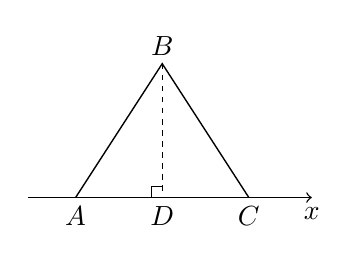
\begin{tikzpicture}[scale=1,line width=0.5pt]
\draw[->] (-0.4,0) -- (3.2,0) node[below] {$x$};
\draw (0.2,0) -- (1.3,1.7) -- (2.4,0);
\node at (0.2,-0.24) {$A$};
\node at (1.3,-0.24) {$D$};
\node at (2.4,-0.24) {$C$};
\node at (1.3,1.92) {$B$};
\draw[dash pattern=on 2pt off 2pt] (1.3,1.7) -- (1.3,0);
\draw (1.16,0) -- (1.16,0.14) -- (1.3,0.14);
\end{tikzpicture}
\end{center}
\step{$AB=AC=BC=\dfrac{2\sqrt3}3$，则 $x_2=x_1+AD=x_1+\dfrac{\sqrt3}3$，$x_3=x_1+\dfrac{2\sqrt3}3$，}
\step{存在 $x_1=-\dfrac{\sqrt3}3$，使得 $x_2=x_1+\dfrac{\sqrt3}3=0\in\Q$，且 $x_3=x_1+\dfrac{2\sqrt3}3=\dfrac{\sqrt3}3$ 为无理数，}
\step{即 $D(x_2)=1$，$D(x_3)=0$ 与图形一致，符合题意，}
\step{此时，$S_{\triangle ABC}=\dfrac12AC\cdot BD=\dfrac{\sqrt3}3$.}
\step{综上所述，存在这样的点 $A$、$B$、$C$，该正三角形的面积为 $\dfrac{\sqrt3}3$.}
\solend

\fi

\item 已知函数 $f(x)$ 满足：对 $\forall x\in R$，都有 $f(x+2025)\leqslant f(x)+2026$，
$f(x+2026)\geqslant f(x)+2027$，若 $f(1)=0$，则 $f(2)$ 的取值范围是\blankline[4.4em].

\ifanswer
\solbegin
\step{对 $\forall x\in R$，都有 $f(x+2025)\leqslant f(x)+2026$，$f(x+2026)\geqslant f(x)+2027$，}
\step{则 $f(x)+2027\leqslant f(x+2026)=f(x+1+2025)\leqslant f(x+1)+2026$，}
\step{即 $f(x)+1\leqslant f(x+1)$，所以 $f(2)\geqslant f(1)+1=1$；}
\step{$f(x)+2026\geqslant f(x+2025)=f(x+2024+1)\geqslant f(x+2024)+1$}
\step{$\geqslant\cdots\geqslant f(x+1)+2024$，所以 $f(x)+2\geqslant f(x+1)$，}
\step{所以 $f(2)\leqslant f(1)+2=2$；}
\step{即 $f(2)$ 的取值范围是 $[1,2]$.}
\solend

\fi

\end{enumerate}

\bigsec{二、选择题}

\begin{enumerate}
\setcounter{enumi}{12}

\item 若实数 $0<m<n<1$，而实数 $x>1$，则下列不等式正确的是\mbox{（\quad）}

\keepwithprev
A. $m^x<n^x$\qquad\qquad B. $x^m>x^n$\qquad\qquad C. $\log_xm>\log_xn$\qquad D. $\log_mx<\log_nx$

\ifanswer
\solbegin
\step{对于 $A$，函数 $f(t)=t^x$ 是以 $t$ 为变量，$x$ 为常量的幂函数，}
\step{由于 $x>1$，易得 $f(t)$ 在 $(0,+\infty)$ 上严格增，}
\step{$0<m<n<1$，$x>1$，可以得到 $m^x<n^x$，故 $A$ 正确；}
\step{对于 $B$，函数 $g(s)=x^s$，是以 $s$ 为变量，$x$ 为常量的指数函数，}
\step{由于 $x>1$，则 $g(s)$ 严格增，$0<m<n<1$，可以得到 $x^m<x^n$，故 $B$ 不正确；}
\step{对于 $C$，$\log_xm=\dfrac{\lg m}{\lg x}$，$\log_xn=\dfrac{\lg n}{\lg x}$，由于 $0<m<n<1$，则 $\lg m<\lg n<0$，}
\step{$x>1$，则 $\lg x>0$，则有 $\dfrac{\lg m}{\lg x}<\dfrac{\lg n}{\lg x}$，即 $\log_xm<\log_xn$，故 $C$ 不正确；}
\step{对于 $D$，由 $\log_mx-\log_nx=\dfrac{\lg x}{\lg m}-\dfrac{\lg x}{\lg n}=\dfrac{\lg x(\lg n-\lg m)}{\lg m\lg n}$，}
\step{因为实数 $0<m<n<1$，而实数 $x>1$，}
\step{所以 $\lg x>0$，$\lg m<\lg n<0$，则 $\dfrac{\lg x(\lg n-\lg m)}{\lg m\lg n}>0$，即 $\log_mx>\log_nx$，}
\step{故 $D$ 不正确.}
\step{故选 $A$.}
\solend

\fi

\item 已知 $x>1$，$y>1$，则 “$4^x>2^y$” 是 $\log_2x>\log_4(y-1)$ ”的\mbox{（\quad）}

\keepwithprev
A. 充分不必要条件\qquad\qquad B. 必要不充分条件

C. 充要条件\qquad\qquad D. 既不充分也不必要条件

\ifanswer
\solbegin
\step{因为 $x>1$，$y>1$，若 $4^x>2^y$，即 $2^{2x}>2^y$，所以 $2x>y>1$，}
\step{因为 $\dfrac y2-\sqrt{y-1}=\dfrac{(\sqrt{y-1})^2-2\sqrt{y-1}+1}2=\dfrac{(\sqrt{y-1}-1)^2}2\geqslant0$，}
\step{即 $\dfrac y2\geqslant\sqrt{y-1}>0$，所以 $\log_2\dfrac y2\geqslant\log_2\sqrt{y-1}=\dfrac12\log_2(y-1)=\log_4(y-1)$，}
\step{又 $x>\dfrac y2>\dfrac12$，所以 $\log_2x>\log_2\dfrac y2\geqslant\log_4(y-1)$，故充分性成立；}
\step{取 $x=2$，$y=4$，满足 $1=\log_2x>\log_4(y-1)=\log_43$，}
\step{但 $16=4^x=2^y=16$，即不满足 $4^x>2^y$，故必要性不成立.}% 链首链尾两个 16 系原卷笔误，应为 4^x=2^y=16，照录
\step{故选 $A$.}
\solend

\fi

\item 以下命题中，真命题的个数是\mbox{（\quad）}

①函数 $y=(x^2+1)^2+3$ 最小值为 3；②若 $2^a+\log_2a=4^b+2\log_4b$，则 $a<2b$；③不等式
$2^x-x-1>0$ 的解集为 $(1,+\infty)$.

\keepwithprev
A. $0$\qquad\qquad B. $1$\qquad\qquad C. $2$\qquad\qquad D. $3$

\ifanswer
\solbegin
\step{对于①，由于 $x^2+1\geqslant1$，则 $y=(x^2+1)^2+3\geqslant4$，}
\step{即函数 $y=(x^2+1)^2+3$ 最小值为 4，①错误；}
\step{对于②，由于 $b>0$，}
\step{则有 $2^a+\log_2a=4^b+2\log_4b=2^{2b}+\log_2b<2^{2b}+\log_22b$，}
\step{设 $f(x)=2^x+\log_2x$，易得 $f(x)$ 在 $(0,+\infty)$ 上为严格增函数，必有 $a<2b$，}
\step{②正确；}
\step{对于③，当 $x=-1$ 时，$2^x-x-1=2^x(x+1)>0$，即 $-1$ 在不等式的解集内，}
\step{③错误；}
\step{故选 $B$.}
\solend

\fi

\item 已知函数 $f(x)=ax^2+bx+c$（$a\neq0$ 且 $a<b$），若对任意的 $x\in R$，$f(x)\geqslant0$，且
$f(1)\geqslant\lambda(b-a)$，则实数 $\lambda$ 的取值范围为\mbox{（\quad）}

\keepwithprev
A. $(-\infty,2]$\qquad\qquad B. $[2\text{，}+\infty)$\qquad\qquad C. $(-\infty\text{，}3]$\qquad\qquad D. $[3\text{，}+\infty)$% 原卷 B/C/D 用全角逗号、A 用半角，照录

\ifanswer
\solbegin
\step{因为函数 $f(x)\geqslant0$ 恒成立，所以 $a>0$，且 $\Delta=b^2-4ac\leqslant0$，即 $c\geqslant\dfrac{b^2}{4a}$，}
\step{所以 $a+b+c\geqslant a+b+\dfrac{b^2}{4a}$，又 $a<b$，所以 $b-a>0$，}
\step{又 $f(1)\geqslant\lambda(b-a)$ 恒成立，所以 $a+b+c\geqslant\lambda(b-a)$ 恒成立，}
\step{即 $\lambda\leqslant\left(\dfrac{a+b+c}{b-a}\right)_{\min}=\dfrac{a+b+\dfrac{b^2}{4a}}{b-a}$，}
\step{令 $t=\dfrac ba$（$t>1$），则 $\dfrac{a+b+\dfrac{b^2}{4a}}{b-a}=\dfrac{1+t+\dfrac{t^2}4}{t-1}$，}
\step{令 $\mu=t-1$（$\mu>0$），则 $t=\mu+1$，}
\step{故上式 $=\dfrac{1+\mu+1+\dfrac{(\mu+1)^2}4}{\mu}=\dfrac14\left(\mu+\dfrac9\mu+6\right)$，}
\step{对 $\mu>0$，有 $\mu+\dfrac9\mu\geqslant2\sqrt{\mu\times\dfrac9\mu}=6$，当且仅当 $\mu=\dfrac9\mu$，即 $\mu=3$ 时取等号，}
\step{所以 $\dfrac14\left(\mu+\dfrac9\mu+6\right)\geqslant\dfrac14(6+6)=3$，故 $\lambda\leqslant3$，}
\step{即实数 $\lambda$ 的取值范围为 $(-\infty,3]$. 故选 $C$.}
\solend

\fi

\end{enumerate}

\bigsec{三、解答题}

\begin{enumerate}
\setcounter{enumi}{16}

\item 已知函数 $f(x)=\log_\frac23(ax^2-6x+18)$.

（1）若 $f(x)$ 的定义域为 $R$，求实数 $a$ 的取值范围.

（2）若 $f(x)$ 的值域为 $R$，求实数 $a$ 的取值范围.

\ansspace*[10]

\ifanswer
\solbegin
\stepm{（1）}{由 $f(x)=\log_\frac23(ax^2-6x+18)$ 的定义域为 $R$，得 $ax^2-6x+18>0$ 恒成立，}
\step{$a=0$ 时，$f(x)=\log_\frac23(18-6x)$ 的定义域为 $(-\infty,3)$，不符合题意.}
\step{$a\neq0$ 时，$\begin{cases}a>0\\ \Delta=36-4\times18a<0\end{cases}$，解得 $a>\dfrac12$.}
\step{综上，$a$ 的取值范围是 $\left(\dfrac12,+\infty\right)$.}
\stepm{（2）}{$a=0$ 时，$f(x)=\log_\frac23(18-6x)$ 的值域为 $R$，符合题意.}
\step{$a\neq0$ 时，$\begin{cases}a>0\\ \Delta=36-4\times18a\geqslant0\end{cases}$，解得 $0<a\leqslant\dfrac12$.}
\step{综上，$a$ 的取值范围是 $\left[0,\dfrac12\right]$.}
\solend

\fi

\item 已知 $f(x)=\log_ax+\log_a(6-x)$，$a>0$ 且 $a\neq1$，且 $f(3)=2$.

（1）求 $a$ 的值及 $f(x)$ 的单调区间.

（2）若对于 $\forall x_1\in(0,6)$，$\exists x_2\in[1,9]$，使得 $f(x_1)\leqslant t+\log_3x_2$ 成立，求实数 $t$ 的取值范
围.

\ansspace*[12]

\ifanswer
\solbegin
\stepm{（1）}{已知 $f(x)=\log_ax+\log_a(6-x)$，且 $f(3)=2$.}
\step{得 $\log_a3+\log_a(6-3)=2$，即 $2\log_a3=2$，}
\step{因此 $\log_a3=1$，因此 $a=3$，因此 $f(x)=\log_3x+\log_3(6-x)$，}
\step{因为 $\begin{cases}x>0\\ 6-x>0\end{cases}$，因此 $0<x<6$，故 $f(x)$ 的定义域为 $(0,6)$；}
\step{$f(x)=\log_3(6x-x^2)$，}
\step{因为函数 $y=6x-x^2$ 在 $(0,3)$ 上严格增，在 $(3,6)$ 上严格减，}
\step{又函数 $y=\log_3x$ 为严格增函数，}
\step{由复合函数的单调性得函数 $f(x)$ 在 $(0,3)$ 上严格增，在 $(3,6)$ 上严格减；}
\stepm{（2）}{令 $g(x)=t+\log_3x$，}
\step{因为 $\forall x_1\in(0,6)$，$\exists x_2\in[1,9]$，使得 $f(x_1)\leqslant t+\log_3x_2$，}
\step{即 $f(x_{1})_{\max}\leqslant g(x_{2})_{\max}$，}
\step{其中由（1）得 $f(x_{1})_{\max}=f(3)=2$.}
\step{又 $g(x)=t+\log_3x$ 在 $[1,9]$ 上严格增，因此 $g(x)_{\max}=g(9)=t+2$，}
\step{因此 $2\leqslant t+2$，因此实数 $t$ 的取值范围为 $[0,+\infty)$.}
\solend

\fi

\item 某心理学研究小组在对学生上课注意力集中情况的调查研究中，发现其注意力指数 $p$ 与
听课时间 $t$ 之间的关系满足如图所示的曲线. 当 $t\in(0,14]$ 时，曲线是二次函数图象的一部
分，当 $t\in[14,40]$ 时，曲线是函数 $y=\log_a(t-5)+83$（$a>0$ 且 $a\neq1$）图象的一部分. 根据
专家研究，当注意力指数 $p$ 大于等于 80 时听课效果最佳.

（1）试求 $p=f(t)$ 的函数关系式；

（2）当一位学生在坚持听课 32 分钟时，注意力指数 $p$ 大约为多少？

（3）一道数学难题，讲解需要 20 分钟，问老师能否经过合理安排在学生听
课效果最佳时讲完？请说明理由.

\begin{center}
% 原图第 9 页题干 p-t 曲线图按原图形状用 TikZ 重排（三版都出）。
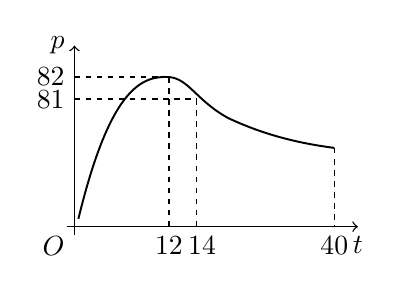
\begin{tikzpicture}[scale=1,line width=0.5pt]
\draw[->] (-0.1,0) -- (3.6,0) node[below] {$t$};
\draw[->] (0,-0.1) -- (0,2.3) node[left] {$p$};
\node[below left] at (0,0) {$O$};
\draw[line width=0.7pt] (0.05,0.1) .. controls (0.45,1.75) and (0.85,1.92) .. (1.2,1.9)
  .. controls (1.45,1.88) and (1.55,1.6) .. (1.95,1.38)
  .. controls (2.5,1.12) and (3.0,1.04) .. (3.3,1.0);
\draw[dash pattern=on 2pt off 2pt] (0,1.9) -- (1.2,1.9);
\draw[dash pattern=on 2pt off 2pt] (0,1.62) -- (1.55,1.62);
\draw[dash pattern=on 2pt off 2pt] (1.2,1.9) -- (1.2,0);
\draw[dash pattern=on 2pt off 2pt] (1.55,1.62) -- (1.55,0);
\draw[dash pattern=on 2pt off 2pt] (3.3,1.0) -- (3.3,0);
\node[left] at (0,1.9) {$82$};
\node[left] at (0,1.62) {$81$};
\node[below] at (1.2,0) {$12$};
\node[below] at (1.62,0) {$14$};
\node[below] at (3.3,0) {$40$};
\end{tikzpicture}
\end{center}

\ansspace*[12]

\ifanswer
\solbegin
\stepm{（1）}{由题意得当 $t\in(0,14]$ 时，设 $f(t)=c(t-12)^2+82$（$c<0$），}
\step{又 $f(14)=81$，所以 $c(14-12)^2+82=81$，解得 $c=-\dfrac14$；}
\step{所以 $f(t)=-\dfrac14(t-12)^2+82$,$t\in(0,14]$；}
\step{又当 $t\in[14,40]$ 时，函数 $y=\log_a(t-5)+83$（$a>0$ 且 $a\neq1$），}
\step{又当 $x=14$ 时，$y=81$，所以 $81=\log_a(14-5)+83$，解得 $a=\dfrac13$；}
\step{所以 $f(t)=\log_\frac13(t-5)+83$,$t\in[14,40]$，}
\step{所以 $p=\begin{cases}-\dfrac14(t-12)^2+82, & t\in(0,14]\\ \log_\frac13(t-5)+83, & t\in(14,40]\end{cases}$；}
\stepm{（2）}{当 $t=32$ 时，$p=\log_\frac13(32-5)+83=80$，}
\step{所以当一位学生在坚持听课 32 分钟时，注意力指数 $p$ 大约为 80；}
\stepm{（3）}{当 $t\in(0,14]$ 时，$-\dfrac14(t-12)^2+82\geqslant80$，解得 $t\in[12-2\sqrt2,14]$，}
\step{当 $t\in[14,40]$ 时，$\log_\frac13(t-5)+83\geqslant80$，解得 $5<t\leqslant32$，则 $t\in[14,32]$，}
\step{因此当 $t\in[12-2\sqrt2,32]$ 时学生听课效果最佳，}
\step{此时 $\Delta t=32-(12-2\sqrt2)=20+2\sqrt2>20$，}
\step{所以老师能经过合理安排时间在学生听课效果最佳时段讲完.}
\solend

\fi

\item 已知 $a\in R$，函数 $f(x+1)=\log_2\left(\dfrac{ax+1+a}{x+1}\right)$.

（1）若 $a=2$，求函数 $f(x)$ 的表达式及定义域；

（2）若关于 $x$ 的方程 $f\left(\dfrac x2\right)-\log_2[(a-2)x+3a-5]=0$ 的解集中恰好只有一个元素，求实
数 $a$ 的取值范围.

\ansspace*[14]

\ifanswer
\solbegin
\stepm{（1）}{$f(x+1)=\log_2\left(\dfrac{ax+1+a}{x+1}\right)$，}
\step{令 $x+1=t$，则 $f(t)=\log_2\left(\dfrac1t+a\right)$，即 $f(x)=\log_2\left(\dfrac1x+a\right)$，}
\step{因为 $a=2$，所以 $f(x)=\log_2\left(2+\dfrac1x\right)$，}
\step{由 $2+\dfrac1x>0$ 得定义域为 $\left(-\infty,-\dfrac12\right)\cup(0,+\infty)$；}
\stepm{（2）}{由（1）得 $f(x)=\log_2\left(\dfrac1x+a\right)$，}
\step{方程 $f\left(\dfrac x2\right)-\log_2[(a-2)x+3a-5]=0$，}
\step{即 $\log_2\left(\dfrac2x+a\right)-\log_2[(a-2)x+3a-5]=0$，}
\step{可转化为 $(a-2)x^2+(2a-5)x-2=0$，且 $\dfrac2x+a>0$.}
\step{①当 $a-2=0$，即 $a=2$ 时，$x=-2$，符合题意；}
\step{②当 $a-2\neq0$，即 $a\neq2$ 时，$x_1=-2$,$x_2=\dfrac1{a-2}$，}
\step{（$i$）当 $-2=\dfrac1{a-2}$ 时，即 $a=\dfrac32$ 时，符合题意；}
\step{（$ii$）当 $-2\neq\dfrac1{a-2}$ 时，即 $a\neq\dfrac32$ 且 $a\neq2$ 时，}
\step{要满足题意，则有 $\begin{cases}-1+a>0\\ 3a-4\leqslant0\end{cases}\Rightarrow1<a\leqslant\dfrac43$ 或 $\begin{cases}-1+a\leqslant0\\ 3a-4>0\end{cases}$，无解；}
\step{综上，$a$ 的取值范围 $\left(1,\dfrac43\right]\cup\left\{2,\dfrac32\right\}$.}
\solend

\fi

\item 已知函数 $y=f(x)$ 是定义在 $[0,+\infty)$ 上的函数，并且 $f(x)\geqslant0$，对于定义域内的任意自
变量的值 $x$、$y$，满足 $f(y)f(x^2f(y)+xf(y))=f(x^2+y+x)$，$f(a)=0$，其中
$a>0$.

（1）当 $f(0)\neq0$ 时，求 $f(0)$；

（2）已知当 $0\leqslant x<a$ 时，有 $f(x)\neq0$.

（$i$）求 $f(a+3)$；

（$ii$）求函数 $y=f(x)$ 的解析式（用 $a$ 表示）.

\ansspace*[16]

\ifanswer
\solbegin
\stepm{（1）}{因为 $f(x)\geqslant0$，且对于定义域内的任意自变量的值 $x$、$y$，}
\step{满足 $f(y)f(x^2f(y)+xf(y))=f(x^2+y+x)$，}
\step{令 $x=y=0$，则 $f^2(0)=f(0)$，因为 $f(0)\neq0$，所以 $f(0)=1$，}
\stepm{（2）}{（$i$）由 $f(y)f(x^2f(y)+xf(y))=f(x^2+y+x)$，}
\step{得 $f(y)f[(x^2+x)f(y)]=f[(x^2+x)+y]$，}
\step{令 $t=x^2+x$，因为 $x\geqslant0$，所以 $t=x^2+x\in[0,+\infty)$，}
\step{所以有 $f(y)f(tf(y))=f(t+y)$，因为 $f(a)=0$，}
\step{令 $y=a$，$t=3$，得 $f(a+3)=f(a)f(3f(a))=0\times f(3f(a))=0$；}
\step{（$ii$）当 $x\geqslant a$ 时，令 $y=a$，$t=x-a$，}
\step{$f(x)=f(x-a+a)=f(a)f[(x-a)f(a)]=0$.}
\step{当 $0\leqslant x<a$ 时，则有 $0<a-x\leqslant a$，令 $y=x$，$t=a-x$，}
\step{则 $f(a)=f(a-x+x)=f(x)f[(a-x)f(x)]=0$.}
\step{因为 $f(x)\neq0$，所以有 $f((a-x)f(x))=0$，则 $(a-x)f(x)\geqslant a$，}
\step{又因为 $a-x>0$，即 $f(x)\geqslant\dfrac a{a-x}$.}
\step{令 $t=\dfrac a{f(x)}>0$,$y=x>0$，}
\step{则 $f\left(\dfrac a{f(x)}+x\right)=f(x)\cdot f\left(\dfrac a{f(x)}\cdot f(x)\right)=f(x)\cdot f(a)=0$，}
\step{所以有 $\dfrac a{f(x)}+x\geqslant a$，即 $\dfrac a{f(x)}\geqslant a-x$，得 $f(x)\leqslant\dfrac a{a-x}$，}
\step{所以当 $0\leqslant x<a$ 时，$f(x)=\dfrac a{a-x}$.}
\step{综上，$f(x)=\begin{cases}\dfrac a{a-x}, & 0\leqslant x<a\\ 0, & x\geqslant a\end{cases}$.}
\solend

\fi

\end{enumerate}

\end{document}
"
% 紧凑版：xelatex "\def\iscompact{1}% 高一105_交附闵行_周末作业10.30.tex
%   —— 高一上数学“2026-2027 年交附闵行高一上周末作业 10.30”（试卷版/答案版）
% 试卷版：xelatex 高一105_交附闵行_周末作业10.30.tex
% 答案版：xelatex "\def\isanswer{1}% 高一105_交附闵行_周末作业10.30.tex
%   —— 高一上数学“2026-2027 年交附闵行高一上周末作业 10.30”（试卷版/答案版）
% 试卷版：xelatex 高一105_交附闵行_周末作业10.30.tex
% 答案版：xelatex "\def\isanswer{1}\input{高一105_交附闵行_周末作业10.30.tex}"
% 紧凑版：xelatex "\def\iscompact{1}\input{高一105_交附闵行_周末作业10.30.tex}"
%
% 原始材料：微信公众号“魔都数学加油站”文章，作者破晓，2026-11-02 17:41 发布；
% 连载“27学年高一105”，原文标题“27学年高一105——2026-2027年上海市交附闵行高一上周末作业10.30”；
% 原文链接：https://mp.weixin.qq.com/s/XUfNEvGHjD0CB5jdoleBWw。
% 正文为 13 张 PNG 页（第 4、9、13 页 2560×3620，其余 4762×6735），题目下印有【解析】，为讲评版。
% 题目、解析均据原图转录；卷面水印及公众号页脚未录入。
%
% 卷首标题：原卷印作“2026-2027 年交附闵行高一上周末作业 10.30”（公众号标题中的“上海市”
% 卷面标题行没有，本稿照卷面），年份区间按全稿惯例排 en dash；原卷未印副标题，本稿按题目
% 内容标为“函数、不等式”（主体为指数与对数，第 3 题集合、第 16 题基本不等式）。
%
% 与原卷的排版差异：
%   ① 原文从第 3 题起，填空题编号为 3—12、选择题为 13—16、解答题为 17—21，本稿保留原题号；
%   ② 原卷每题下直接印【解析】，本稿按全稿惯例将解析置于答案版；选择题括号内未印答案，另由
%      解析末句“故选 X”给出；
%   ③ 原卷未印副标题，本稿按“知识模块”口径补出；
%   ④ 原卷填空横线按全稿惯例排为 \blankline[4.4em]；解答题按惯例加 \ansspace；选择题括号排
%      \mbox{（\quad）}、选项段前按惯例加 \keepwithprev；
%   ⑤ $f(x_1)_{max}$、$g(x)_max$、$\left(\frac{a+b+c}{b-a}\right)_{min}$ 等下标原卷排斜体，
%      按 高一96 成例改正体 $\max$、$\min$；
%   ⑥ 原卷数集排斜体 $R$／$Q$，按全稿惯例改 $\R$／$\Q$；
%   ⑦ 第 11 题解析的两幅三角形示意图与第 19 题题干的 $p$-$t$ 曲线图均按原图形状用 TikZ 重排
%      （第 19 题图属题干、三版都出；第 11 题图属解析、仅答案版显示）。
%
% 原卷存疑／笔误（均照录加注）：
%   第 14 题解析“但 $16=4^x=2^y=16$”（链首、链尾的两个 $16$ 系原卷笔误，按上下文应为
%   $4^x=2^y=16$）；
%   第 16 题选项的区间分隔逗号 A 项排半角、B／C／D 三项排全角（原卷自身不一致）；
%   第 21 题 (2) 的小问号排“（$i$）求…”（右括号紧贴“求”字），照录。
%
% 行数核对：逐题数 \step/\stepm 条数，合计 159 条（Q3：2；Q4：1；Q5：4；Q6：6；Q7：3；
% Q8：7；Q9：5；Q10：3；Q11：15；Q12：7；Q13：12；Q14：7；Q15：9；Q16：10；Q17：7；
% Q18：14；Q19：14；Q20：14；Q21：19），与原卷印刷行逐题相等。
%
\documentclass[a4paper,11pt]{article}
\usepackage{common}

\begin{document}

\examtitlest[3]{2026--2027 年交附闵行高一上周末作业 10.30}{函数、不等式}

\bigsec{一、填空题}

\begin{enumerate}
\setcounter{enumi}{2}

\item 已知集合 $M=\{1,m\}$，$N=\{n,\log_2n\}$，若 $M=N$，则 $(m-n)^{2027}=$\blankline[4.4em].

\ifanswer
\solbegin
\step{由题意得 $\begin{cases}n=1\\ \log_2n=m\end{cases}$ 或 $\begin{cases}n=m\\ \log_2n=1\end{cases}$，解得 $\begin{cases}n=1\\ m=0\end{cases}$ 或 $\begin{cases}n=2\\ m=2\end{cases}$，}
\step{所以 $(m-n)^{2027}=-1$ 或 $0$.}
\solend

\fi

\item 已知 $\log_{2x^2-1}(3x^2+2x-1)=1$，则 $x=$\blankline[4.4em].

\ifanswer
\solbegin
\step{因为 $\log_{2x^2-1}(3x^2+2x-1)=1$，所以 $\begin{cases}2x^2-1>0\\ 2x^2-1\neq1\\ 3x^2+2x-1>0\\ 2x^2-1=3x^2+2x-1\end{cases}$，解得 $x=-2$.}
\solend

\fi

\item 已知 $m>1$，$n>1$，$\lg m=\log_n100$，则 $mn$ 的最小值为\blankline[4.4em].

\ifanswer
\solbegin
\step{由 $m>1$，$n>1$，得 $\lg m>0$，$\lg n>0$，}
\step{因为 $\lg m=\log_n100=\dfrac{\lg100}{\lg n}=\dfrac2{\lg n}$，所以 $\lg m\cdot\lg n=2$，}
\step{所以 $\lg(mn)=\lg m+\lg n\geqslant2\sqrt{\lg m\cdot\lg n}=2\sqrt2$，}
\step{当且仅当 $m=n=10^{\sqrt2}$ 时取等号，则 $mn\geqslant10^{2\sqrt2}$，即 $mn$ 的最小值为 $10^{2\sqrt2}$.}
\solend

\fi

\item 设 $m$、$n$ 分别是方程 $\log_{2013}x+x-9=0$ 和 $2013^x+x-9=0$ 的根，则 $m+n=$\blankline[4.4em].

\ifanswer
\solbegin
\step{由 $\log_{2013}x+x-9=0$，得 $\log_{2013}x=-x+9$，}
\step{因为 $m$ 是方程 $\log_{2013}x+x-9=0$ 的根，}
\step{所以 $m$ 为函数 $y=\log_{2013}x$ 与 $y=-x+9$ 图象交点的横坐标，}
\step{同理 $n$ 是函数 $y=2013^x$ 与 $y=-x+9$ 图象交点的横坐标，}
\step{因为 $y=\log_{2013}x$ 与 $y=2013^x$ 互为反函数，其图象关于直线 $y=x$ 对称，}
\step{联立 $\begin{cases}y=-x+9\\ y=x\end{cases}$，解得 $x=\dfrac92$，所以 $m+n=\dfrac92\times2=9$.}
\solend

\fi

\item 已知函数 $f(x)=\dfrac1{\log_2(x^2+4)}$，则 $f(-2)=$\blankline[2em]，$f(x)$ 的值域为\blankline[4.4em].

\ifanswer
\solbegin
\step{$f(-2)=\dfrac1{\log_28}=\dfrac13$.}
\step{因为 $x^2+4\geqslant4$，所以 $\log_2(x^2+4)\geqslant\log_24=2$，所以 $0<\dfrac1{\log_2(x^2+4)}\leqslant\dfrac12$，}
\step{故 $f(x)$ 的值域为 $\left(0,\dfrac12\right]$.}
\solend

\fi

\item 已知 $\alpha$、$\beta$ 是方程 $9^x-2m\cdot3^x+m^2-1=0$ 的两个根，若 $\alpha+\beta=1$，则 $\alpha\beta=$\blankline[4.4em].

\ifanswer
\solbegin
\step{由题意得方程 $9^x-2m\cdot3^x+m^2-1=0$ 有两个根，}
\step{则方程 $t^2-2mt+m^2-1=0$ 有二正根，}
\step{则 $\begin{cases}\Delta=4m^2-4(m^2-1)\geqslant0\\ 2m>0\\ m^2-1>0\end{cases}$，解得 $m>1$，}
\step{又 $\alpha$、$\beta$ 是方程 $9^x-2m\cdot3^x+m^2-1=0$ 的两个根，}
\step{则 $3^\alpha\times3^\beta=m^2-1$，又 $\alpha+\beta=1$，则 $m^2-1=3^{\alpha+\beta}=3$，}
\step{解得 $m=2$ 或 $m=-2$（舍），则 $3^\alpha+3^\beta=2m=4$，又 $\alpha=1-\beta$，}
\step{则 $3^{1-\beta}+3^\beta=4$，解得 $\beta=0$ 或 $\beta=1$，则 $\begin{cases}\alpha=1\\ \beta=0\end{cases}$ 或 $\begin{cases}\alpha=0\\ \beta=1\end{cases}$，则 $\alpha\beta=0$.}
\solend

\fi

\item 已知 $a>b>0$，$\ln a=2\ln b$，且 $a\lg b=b\lg a$，则 $a+b=$\blankline[4.4em].

\ifanswer
\solbegin
\step{因为 $a>b>0$，$\ln a=2\ln b=\ln b^2$，所以 $a=b^2$，}
\step{由 $a\lg b=b\lg a$ 得 $b^2\lg b=b\lg b^2$，即 $b\lg b=2\lg b$，所以 $b=1$ 或 $b=2$，}
\step{当 $b=2$，$a=4$，满足题意，}
\step{当 $b=1$ 时，$a=1$ 与 $a>b>0$ 矛盾，所以 $b=1$ 舍去，}
\step{所以 $a+b=6$.}
\solend

\fi

\item 函数 $f(x)=\begin{cases}2^x, & x\leqslant t\\ \log_\frac12x, & x>t\end{cases}$ 的值域为 $M$，且 $8\notin M$，则实数 $t$ 的取值集合为\blankline[4.4em].

\ifanswer
\solbegin
\step{当 $x\leqslant t$ 时，函数 $f(x)=2^x$ 在 $(-\infty,t]$ 严格增，}
\step{当 $x>t$ 时，$f(x)=\log_\frac12x$ 在 $(t,+\infty)$ 严格减，}
\step{若 $8\notin M$，则满足条件 $\begin{cases}2^t<8\\ \log_\frac12t\leqslant8\end{cases}\Rightarrow\dfrac1{256}\leqslant t<3$，故实数 $t$ 的取值集合为 $\left[\dfrac1{256},3\right)$.}
\solend

\fi

\item 德国数学家狄利克雷在数学领域成就显著，以其命名函数 $D(x)=\begin{cases}1, & x\text{为有理数}\\ 0, & x\text{为无理数}\end{cases}$，该函
数被称为狄利克雷函数。那么是否存在三个点 $A(x_1,D(x_1))$、$B(x_2,D(x_2))$、$C(x_3,D(x_3))$，
使得 $\triangle ABC$ 为等边三角形，若不存在请在横线上填写“不存在”，如果存在则在横线上填写
该正三角形的面积\blankline[4.4em].

\ifanswer
\solbegin
\step{因为 $D(x)=\begin{cases}1, & x\text{为有理数}\\ 0, & x\text{为无理数}\end{cases}$，所以 $D(x)=0$ 或 1，}
\step{设存在三个点 $A(x_1,D(x_1))$、$B(x_2,D(x_2))$、$C(x_3,D(x_3))$，}
\step{使得 $\triangle ABC$ 为等边三角形，则 $D(x_1)$、$D(x_2)$、$D(x_3)$ 不同时为 0 或 1，}
\step{不妨设 $x_1<x_2<x_3$，分析得 $\triangle ABC$ 的位置有两种情况，}
\step{第一种情况：当 $x_1$ 为有理数时，即 $D(x_1)=1$，如图，过点 $B$ 作 $BD\perp AC$，}
\begin{center}
% 原图第 4 页解析示意图按原图形状用 TikZ 重排（第一种情况：$B$ 在 $x$ 轴上、$AC$ 在上方）。
\begin{tikzpicture}[scale=1,line width=0.5pt]
\draw (0,1.2) -- (2.6,1.2);
\node at (0.25,1.4) {$A$};
\node at (1.3,1.4) {$D$};
\node at (2.35,1.4) {$C$};
\draw[dash pattern=on 2pt off 2pt] (1.3,1.2) -- (1.3,0);
\draw (1.16,1.2) -- (1.16,1.06) -- (1.3,1.06);
\draw[->] (-0.5,0) -- (3.1,0) node[below] {$x$};
\node at (1.3,-0.24) {$B$};
\end{tikzpicture}
\end{center}
\step{垂足为 $D$，得 $BD=1$，$AD=\dfrac{\sqrt3}3$，$AB=AC=BC=\dfrac{2\sqrt3}3$，}
\step{则 $x_2=x_1+AD=x_1+\dfrac{\sqrt3}3$ 为无理数，$x_3=x_1+\dfrac{2\sqrt3}3$ 为无理数，}
\step{即 $D(x_2)=0$，$D(x_3)=0$ 与图形不一致，舍去；}
\step{第二种情况：当 $x_1$ 为无理数时，即 $D(x_1)=0$，如图，}
\step{过点 $B$ 作 $BD\perp AC$，垂足为 $D$，得 $BD=1$，$AD=\dfrac{\sqrt3}3$，}
\begin{center}
% 原图第 4 页解析示意图按原图形状用 TikZ 重排（第二种情况：$B$ 在上方、$AC$ 在 $x$ 轴上）。
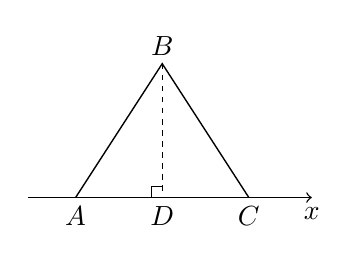
\begin{tikzpicture}[scale=1,line width=0.5pt]
\draw[->] (-0.4,0) -- (3.2,0) node[below] {$x$};
\draw (0.2,0) -- (1.3,1.7) -- (2.4,0);
\node at (0.2,-0.24) {$A$};
\node at (1.3,-0.24) {$D$};
\node at (2.4,-0.24) {$C$};
\node at (1.3,1.92) {$B$};
\draw[dash pattern=on 2pt off 2pt] (1.3,1.7) -- (1.3,0);
\draw (1.16,0) -- (1.16,0.14) -- (1.3,0.14);
\end{tikzpicture}
\end{center}
\step{$AB=AC=BC=\dfrac{2\sqrt3}3$，则 $x_2=x_1+AD=x_1+\dfrac{\sqrt3}3$，$x_3=x_1+\dfrac{2\sqrt3}3$，}
\step{存在 $x_1=-\dfrac{\sqrt3}3$，使得 $x_2=x_1+\dfrac{\sqrt3}3=0\in\Q$，且 $x_3=x_1+\dfrac{2\sqrt3}3=\dfrac{\sqrt3}3$ 为无理数，}
\step{即 $D(x_2)=1$，$D(x_3)=0$ 与图形一致，符合题意，}
\step{此时，$S_{\triangle ABC}=\dfrac12AC\cdot BD=\dfrac{\sqrt3}3$.}
\step{综上所述，存在这样的点 $A$、$B$、$C$，该正三角形的面积为 $\dfrac{\sqrt3}3$.}
\solend

\fi

\item 已知函数 $f(x)$ 满足：对 $\forall x\in R$，都有 $f(x+2025)\leqslant f(x)+2026$，
$f(x+2026)\geqslant f(x)+2027$，若 $f(1)=0$，则 $f(2)$ 的取值范围是\blankline[4.4em].

\ifanswer
\solbegin
\step{对 $\forall x\in R$，都有 $f(x+2025)\leqslant f(x)+2026$，$f(x+2026)\geqslant f(x)+2027$，}
\step{则 $f(x)+2027\leqslant f(x+2026)=f(x+1+2025)\leqslant f(x+1)+2026$，}
\step{即 $f(x)+1\leqslant f(x+1)$，所以 $f(2)\geqslant f(1)+1=1$；}
\step{$f(x)+2026\geqslant f(x+2025)=f(x+2024+1)\geqslant f(x+2024)+1$}
\step{$\geqslant\cdots\geqslant f(x+1)+2024$，所以 $f(x)+2\geqslant f(x+1)$，}
\step{所以 $f(2)\leqslant f(1)+2=2$；}
\step{即 $f(2)$ 的取值范围是 $[1,2]$.}
\solend

\fi

\end{enumerate}

\bigsec{二、选择题}

\begin{enumerate}
\setcounter{enumi}{12}

\item 若实数 $0<m<n<1$，而实数 $x>1$，则下列不等式正确的是\mbox{（\quad）}

\keepwithprev
A. $m^x<n^x$\qquad\qquad B. $x^m>x^n$\qquad\qquad C. $\log_xm>\log_xn$\qquad D. $\log_mx<\log_nx$

\ifanswer
\solbegin
\step{对于 $A$，函数 $f(t)=t^x$ 是以 $t$ 为变量，$x$ 为常量的幂函数，}
\step{由于 $x>1$，易得 $f(t)$ 在 $(0,+\infty)$ 上严格增，}
\step{$0<m<n<1$，$x>1$，可以得到 $m^x<n^x$，故 $A$ 正确；}
\step{对于 $B$，函数 $g(s)=x^s$，是以 $s$ 为变量，$x$ 为常量的指数函数，}
\step{由于 $x>1$，则 $g(s)$ 严格增，$0<m<n<1$，可以得到 $x^m<x^n$，故 $B$ 不正确；}
\step{对于 $C$，$\log_xm=\dfrac{\lg m}{\lg x}$，$\log_xn=\dfrac{\lg n}{\lg x}$，由于 $0<m<n<1$，则 $\lg m<\lg n<0$，}
\step{$x>1$，则 $\lg x>0$，则有 $\dfrac{\lg m}{\lg x}<\dfrac{\lg n}{\lg x}$，即 $\log_xm<\log_xn$，故 $C$ 不正确；}
\step{对于 $D$，由 $\log_mx-\log_nx=\dfrac{\lg x}{\lg m}-\dfrac{\lg x}{\lg n}=\dfrac{\lg x(\lg n-\lg m)}{\lg m\lg n}$，}
\step{因为实数 $0<m<n<1$，而实数 $x>1$，}
\step{所以 $\lg x>0$，$\lg m<\lg n<0$，则 $\dfrac{\lg x(\lg n-\lg m)}{\lg m\lg n}>0$，即 $\log_mx>\log_nx$，}
\step{故 $D$ 不正确.}
\step{故选 $A$.}
\solend

\fi

\item 已知 $x>1$，$y>1$，则 “$4^x>2^y$” 是 $\log_2x>\log_4(y-1)$ ”的\mbox{（\quad）}

\keepwithprev
A. 充分不必要条件\qquad\qquad B. 必要不充分条件

C. 充要条件\qquad\qquad D. 既不充分也不必要条件

\ifanswer
\solbegin
\step{因为 $x>1$，$y>1$，若 $4^x>2^y$，即 $2^{2x}>2^y$，所以 $2x>y>1$，}
\step{因为 $\dfrac y2-\sqrt{y-1}=\dfrac{(\sqrt{y-1})^2-2\sqrt{y-1}+1}2=\dfrac{(\sqrt{y-1}-1)^2}2\geqslant0$，}
\step{即 $\dfrac y2\geqslant\sqrt{y-1}>0$，所以 $\log_2\dfrac y2\geqslant\log_2\sqrt{y-1}=\dfrac12\log_2(y-1)=\log_4(y-1)$，}
\step{又 $x>\dfrac y2>\dfrac12$，所以 $\log_2x>\log_2\dfrac y2\geqslant\log_4(y-1)$，故充分性成立；}
\step{取 $x=2$，$y=4$，满足 $1=\log_2x>\log_4(y-1)=\log_43$，}
\step{但 $16=4^x=2^y=16$，即不满足 $4^x>2^y$，故必要性不成立.}% 链首链尾两个 16 系原卷笔误，应为 4^x=2^y=16，照录
\step{故选 $A$.}
\solend

\fi

\item 以下命题中，真命题的个数是\mbox{（\quad）}

①函数 $y=(x^2+1)^2+3$ 最小值为 3；②若 $2^a+\log_2a=4^b+2\log_4b$，则 $a<2b$；③不等式
$2^x-x-1>0$ 的解集为 $(1,+\infty)$.

\keepwithprev
A. $0$\qquad\qquad B. $1$\qquad\qquad C. $2$\qquad\qquad D. $3$

\ifanswer
\solbegin
\step{对于①，由于 $x^2+1\geqslant1$，则 $y=(x^2+1)^2+3\geqslant4$，}
\step{即函数 $y=(x^2+1)^2+3$ 最小值为 4，①错误；}
\step{对于②，由于 $b>0$，}
\step{则有 $2^a+\log_2a=4^b+2\log_4b=2^{2b}+\log_2b<2^{2b}+\log_22b$，}
\step{设 $f(x)=2^x+\log_2x$，易得 $f(x)$ 在 $(0,+\infty)$ 上为严格增函数，必有 $a<2b$，}
\step{②正确；}
\step{对于③，当 $x=-1$ 时，$2^x-x-1=2^x(x+1)>0$，即 $-1$ 在不等式的解集内，}
\step{③错误；}
\step{故选 $B$.}
\solend

\fi

\item 已知函数 $f(x)=ax^2+bx+c$（$a\neq0$ 且 $a<b$），若对任意的 $x\in R$，$f(x)\geqslant0$，且
$f(1)\geqslant\lambda(b-a)$，则实数 $\lambda$ 的取值范围为\mbox{（\quad）}

\keepwithprev
A. $(-\infty,2]$\qquad\qquad B. $[2\text{，}+\infty)$\qquad\qquad C. $(-\infty\text{，}3]$\qquad\qquad D. $[3\text{，}+\infty)$% 原卷 B/C/D 用全角逗号、A 用半角，照录

\ifanswer
\solbegin
\step{因为函数 $f(x)\geqslant0$ 恒成立，所以 $a>0$，且 $\Delta=b^2-4ac\leqslant0$，即 $c\geqslant\dfrac{b^2}{4a}$，}
\step{所以 $a+b+c\geqslant a+b+\dfrac{b^2}{4a}$，又 $a<b$，所以 $b-a>0$，}
\step{又 $f(1)\geqslant\lambda(b-a)$ 恒成立，所以 $a+b+c\geqslant\lambda(b-a)$ 恒成立，}
\step{即 $\lambda\leqslant\left(\dfrac{a+b+c}{b-a}\right)_{\min}=\dfrac{a+b+\dfrac{b^2}{4a}}{b-a}$，}
\step{令 $t=\dfrac ba$（$t>1$），则 $\dfrac{a+b+\dfrac{b^2}{4a}}{b-a}=\dfrac{1+t+\dfrac{t^2}4}{t-1}$，}
\step{令 $\mu=t-1$（$\mu>0$），则 $t=\mu+1$，}
\step{故上式 $=\dfrac{1+\mu+1+\dfrac{(\mu+1)^2}4}{\mu}=\dfrac14\left(\mu+\dfrac9\mu+6\right)$，}
\step{对 $\mu>0$，有 $\mu+\dfrac9\mu\geqslant2\sqrt{\mu\times\dfrac9\mu}=6$，当且仅当 $\mu=\dfrac9\mu$，即 $\mu=3$ 时取等号，}
\step{所以 $\dfrac14\left(\mu+\dfrac9\mu+6\right)\geqslant\dfrac14(6+6)=3$，故 $\lambda\leqslant3$，}
\step{即实数 $\lambda$ 的取值范围为 $(-\infty,3]$. 故选 $C$.}
\solend

\fi

\end{enumerate}

\bigsec{三、解答题}

\begin{enumerate}
\setcounter{enumi}{16}

\item 已知函数 $f(x)=\log_\frac23(ax^2-6x+18)$.

（1）若 $f(x)$ 的定义域为 $R$，求实数 $a$ 的取值范围.

（2）若 $f(x)$ 的值域为 $R$，求实数 $a$ 的取值范围.

\ansspace*[10]

\ifanswer
\solbegin
\stepm{（1）}{由 $f(x)=\log_\frac23(ax^2-6x+18)$ 的定义域为 $R$，得 $ax^2-6x+18>0$ 恒成立，}
\step{$a=0$ 时，$f(x)=\log_\frac23(18-6x)$ 的定义域为 $(-\infty,3)$，不符合题意.}
\step{$a\neq0$ 时，$\begin{cases}a>0\\ \Delta=36-4\times18a<0\end{cases}$，解得 $a>\dfrac12$.}
\step{综上，$a$ 的取值范围是 $\left(\dfrac12,+\infty\right)$.}
\stepm{（2）}{$a=0$ 时，$f(x)=\log_\frac23(18-6x)$ 的值域为 $R$，符合题意.}
\step{$a\neq0$ 时，$\begin{cases}a>0\\ \Delta=36-4\times18a\geqslant0\end{cases}$，解得 $0<a\leqslant\dfrac12$.}
\step{综上，$a$ 的取值范围是 $\left[0,\dfrac12\right]$.}
\solend

\fi

\item 已知 $f(x)=\log_ax+\log_a(6-x)$，$a>0$ 且 $a\neq1$，且 $f(3)=2$.

（1）求 $a$ 的值及 $f(x)$ 的单调区间.

（2）若对于 $\forall x_1\in(0,6)$，$\exists x_2\in[1,9]$，使得 $f(x_1)\leqslant t+\log_3x_2$ 成立，求实数 $t$ 的取值范
围.

\ansspace*[12]

\ifanswer
\solbegin
\stepm{（1）}{已知 $f(x)=\log_ax+\log_a(6-x)$，且 $f(3)=2$.}
\step{得 $\log_a3+\log_a(6-3)=2$，即 $2\log_a3=2$，}
\step{因此 $\log_a3=1$，因此 $a=3$，因此 $f(x)=\log_3x+\log_3(6-x)$，}
\step{因为 $\begin{cases}x>0\\ 6-x>0\end{cases}$，因此 $0<x<6$，故 $f(x)$ 的定义域为 $(0,6)$；}
\step{$f(x)=\log_3(6x-x^2)$，}
\step{因为函数 $y=6x-x^2$ 在 $(0,3)$ 上严格增，在 $(3,6)$ 上严格减，}
\step{又函数 $y=\log_3x$ 为严格增函数，}
\step{由复合函数的单调性得函数 $f(x)$ 在 $(0,3)$ 上严格增，在 $(3,6)$ 上严格减；}
\stepm{（2）}{令 $g(x)=t+\log_3x$，}
\step{因为 $\forall x_1\in(0,6)$，$\exists x_2\in[1,9]$，使得 $f(x_1)\leqslant t+\log_3x_2$，}
\step{即 $f(x_{1})_{\max}\leqslant g(x_{2})_{\max}$，}
\step{其中由（1）得 $f(x_{1})_{\max}=f(3)=2$.}
\step{又 $g(x)=t+\log_3x$ 在 $[1,9]$ 上严格增，因此 $g(x)_{\max}=g(9)=t+2$，}
\step{因此 $2\leqslant t+2$，因此实数 $t$ 的取值范围为 $[0,+\infty)$.}
\solend

\fi

\item 某心理学研究小组在对学生上课注意力集中情况的调查研究中，发现其注意力指数 $p$ 与
听课时间 $t$ 之间的关系满足如图所示的曲线. 当 $t\in(0,14]$ 时，曲线是二次函数图象的一部
分，当 $t\in[14,40]$ 时，曲线是函数 $y=\log_a(t-5)+83$（$a>0$ 且 $a\neq1$）图象的一部分. 根据
专家研究，当注意力指数 $p$ 大于等于 80 时听课效果最佳.

（1）试求 $p=f(t)$ 的函数关系式；

（2）当一位学生在坚持听课 32 分钟时，注意力指数 $p$ 大约为多少？

（3）一道数学难题，讲解需要 20 分钟，问老师能否经过合理安排在学生听
课效果最佳时讲完？请说明理由.

\begin{center}
% 原图第 9 页题干 p-t 曲线图按原图形状用 TikZ 重排（三版都出）。
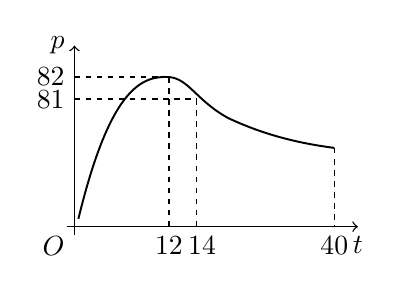
\begin{tikzpicture}[scale=1,line width=0.5pt]
\draw[->] (-0.1,0) -- (3.6,0) node[below] {$t$};
\draw[->] (0,-0.1) -- (0,2.3) node[left] {$p$};
\node[below left] at (0,0) {$O$};
\draw[line width=0.7pt] (0.05,0.1) .. controls (0.45,1.75) and (0.85,1.92) .. (1.2,1.9)
  .. controls (1.45,1.88) and (1.55,1.6) .. (1.95,1.38)
  .. controls (2.5,1.12) and (3.0,1.04) .. (3.3,1.0);
\draw[dash pattern=on 2pt off 2pt] (0,1.9) -- (1.2,1.9);
\draw[dash pattern=on 2pt off 2pt] (0,1.62) -- (1.55,1.62);
\draw[dash pattern=on 2pt off 2pt] (1.2,1.9) -- (1.2,0);
\draw[dash pattern=on 2pt off 2pt] (1.55,1.62) -- (1.55,0);
\draw[dash pattern=on 2pt off 2pt] (3.3,1.0) -- (3.3,0);
\node[left] at (0,1.9) {$82$};
\node[left] at (0,1.62) {$81$};
\node[below] at (1.2,0) {$12$};
\node[below] at (1.62,0) {$14$};
\node[below] at (3.3,0) {$40$};
\end{tikzpicture}
\end{center}

\ansspace*[12]

\ifanswer
\solbegin
\stepm{（1）}{由题意得当 $t\in(0,14]$ 时，设 $f(t)=c(t-12)^2+82$（$c<0$），}
\step{又 $f(14)=81$，所以 $c(14-12)^2+82=81$，解得 $c=-\dfrac14$；}
\step{所以 $f(t)=-\dfrac14(t-12)^2+82$,$t\in(0,14]$；}
\step{又当 $t\in[14,40]$ 时，函数 $y=\log_a(t-5)+83$（$a>0$ 且 $a\neq1$），}
\step{又当 $x=14$ 时，$y=81$，所以 $81=\log_a(14-5)+83$，解得 $a=\dfrac13$；}
\step{所以 $f(t)=\log_\frac13(t-5)+83$,$t\in[14,40]$，}
\step{所以 $p=\begin{cases}-\dfrac14(t-12)^2+82, & t\in(0,14]\\ \log_\frac13(t-5)+83, & t\in(14,40]\end{cases}$；}
\stepm{（2）}{当 $t=32$ 时，$p=\log_\frac13(32-5)+83=80$，}
\step{所以当一位学生在坚持听课 32 分钟时，注意力指数 $p$ 大约为 80；}
\stepm{（3）}{当 $t\in(0,14]$ 时，$-\dfrac14(t-12)^2+82\geqslant80$，解得 $t\in[12-2\sqrt2,14]$，}
\step{当 $t\in[14,40]$ 时，$\log_\frac13(t-5)+83\geqslant80$，解得 $5<t\leqslant32$，则 $t\in[14,32]$，}
\step{因此当 $t\in[12-2\sqrt2,32]$ 时学生听课效果最佳，}
\step{此时 $\Delta t=32-(12-2\sqrt2)=20+2\sqrt2>20$，}
\step{所以老师能经过合理安排时间在学生听课效果最佳时段讲完.}
\solend

\fi

\item 已知 $a\in R$，函数 $f(x+1)=\log_2\left(\dfrac{ax+1+a}{x+1}\right)$.

（1）若 $a=2$，求函数 $f(x)$ 的表达式及定义域；

（2）若关于 $x$ 的方程 $f\left(\dfrac x2\right)-\log_2[(a-2)x+3a-5]=0$ 的解集中恰好只有一个元素，求实
数 $a$ 的取值范围.

\ansspace*[14]

\ifanswer
\solbegin
\stepm{（1）}{$f(x+1)=\log_2\left(\dfrac{ax+1+a}{x+1}\right)$，}
\step{令 $x+1=t$，则 $f(t)=\log_2\left(\dfrac1t+a\right)$，即 $f(x)=\log_2\left(\dfrac1x+a\right)$，}
\step{因为 $a=2$，所以 $f(x)=\log_2\left(2+\dfrac1x\right)$，}
\step{由 $2+\dfrac1x>0$ 得定义域为 $\left(-\infty,-\dfrac12\right)\cup(0,+\infty)$；}
\stepm{（2）}{由（1）得 $f(x)=\log_2\left(\dfrac1x+a\right)$，}
\step{方程 $f\left(\dfrac x2\right)-\log_2[(a-2)x+3a-5]=0$，}
\step{即 $\log_2\left(\dfrac2x+a\right)-\log_2[(a-2)x+3a-5]=0$，}
\step{可转化为 $(a-2)x^2+(2a-5)x-2=0$，且 $\dfrac2x+a>0$.}
\step{①当 $a-2=0$，即 $a=2$ 时，$x=-2$，符合题意；}
\step{②当 $a-2\neq0$，即 $a\neq2$ 时，$x_1=-2$,$x_2=\dfrac1{a-2}$，}
\step{（$i$）当 $-2=\dfrac1{a-2}$ 时，即 $a=\dfrac32$ 时，符合题意；}
\step{（$ii$）当 $-2\neq\dfrac1{a-2}$ 时，即 $a\neq\dfrac32$ 且 $a\neq2$ 时，}
\step{要满足题意，则有 $\begin{cases}-1+a>0\\ 3a-4\leqslant0\end{cases}\Rightarrow1<a\leqslant\dfrac43$ 或 $\begin{cases}-1+a\leqslant0\\ 3a-4>0\end{cases}$，无解；}
\step{综上，$a$ 的取值范围 $\left(1,\dfrac43\right]\cup\left\{2,\dfrac32\right\}$.}
\solend

\fi

\item 已知函数 $y=f(x)$ 是定义在 $[0,+\infty)$ 上的函数，并且 $f(x)\geqslant0$，对于定义域内的任意自
变量的值 $x$、$y$，满足 $f(y)f(x^2f(y)+xf(y))=f(x^2+y+x)$，$f(a)=0$，其中
$a>0$.

（1）当 $f(0)\neq0$ 时，求 $f(0)$；

（2）已知当 $0\leqslant x<a$ 时，有 $f(x)\neq0$.

（$i$）求 $f(a+3)$；

（$ii$）求函数 $y=f(x)$ 的解析式（用 $a$ 表示）.

\ansspace*[16]

\ifanswer
\solbegin
\stepm{（1）}{因为 $f(x)\geqslant0$，且对于定义域内的任意自变量的值 $x$、$y$，}
\step{满足 $f(y)f(x^2f(y)+xf(y))=f(x^2+y+x)$，}
\step{令 $x=y=0$，则 $f^2(0)=f(0)$，因为 $f(0)\neq0$，所以 $f(0)=1$，}
\stepm{（2）}{（$i$）由 $f(y)f(x^2f(y)+xf(y))=f(x^2+y+x)$，}
\step{得 $f(y)f[(x^2+x)f(y)]=f[(x^2+x)+y]$，}
\step{令 $t=x^2+x$，因为 $x\geqslant0$，所以 $t=x^2+x\in[0,+\infty)$，}
\step{所以有 $f(y)f(tf(y))=f(t+y)$，因为 $f(a)=0$，}
\step{令 $y=a$，$t=3$，得 $f(a+3)=f(a)f(3f(a))=0\times f(3f(a))=0$；}
\step{（$ii$）当 $x\geqslant a$ 时，令 $y=a$，$t=x-a$，}
\step{$f(x)=f(x-a+a)=f(a)f[(x-a)f(a)]=0$.}
\step{当 $0\leqslant x<a$ 时，则有 $0<a-x\leqslant a$，令 $y=x$，$t=a-x$，}
\step{则 $f(a)=f(a-x+x)=f(x)f[(a-x)f(x)]=0$.}
\step{因为 $f(x)\neq0$，所以有 $f((a-x)f(x))=0$，则 $(a-x)f(x)\geqslant a$，}
\step{又因为 $a-x>0$，即 $f(x)\geqslant\dfrac a{a-x}$.}
\step{令 $t=\dfrac a{f(x)}>0$,$y=x>0$，}
\step{则 $f\left(\dfrac a{f(x)}+x\right)=f(x)\cdot f\left(\dfrac a{f(x)}\cdot f(x)\right)=f(x)\cdot f(a)=0$，}
\step{所以有 $\dfrac a{f(x)}+x\geqslant a$，即 $\dfrac a{f(x)}\geqslant a-x$，得 $f(x)\leqslant\dfrac a{a-x}$，}
\step{所以当 $0\leqslant x<a$ 时，$f(x)=\dfrac a{a-x}$.}
\step{综上，$f(x)=\begin{cases}\dfrac a{a-x}, & 0\leqslant x<a\\ 0, & x\geqslant a\end{cases}$.}
\solend

\fi

\end{enumerate}

\end{document}
"
% 紧凑版：xelatex "\def\iscompact{1}% 高一105_交附闵行_周末作业10.30.tex
%   —— 高一上数学“2026-2027 年交附闵行高一上周末作业 10.30”（试卷版/答案版）
% 试卷版：xelatex 高一105_交附闵行_周末作业10.30.tex
% 答案版：xelatex "\def\isanswer{1}\input{高一105_交附闵行_周末作业10.30.tex}"
% 紧凑版：xelatex "\def\iscompact{1}\input{高一105_交附闵行_周末作业10.30.tex}"
%
% 原始材料：微信公众号“魔都数学加油站”文章，作者破晓，2026-11-02 17:41 发布；
% 连载“27学年高一105”，原文标题“27学年高一105——2026-2027年上海市交附闵行高一上周末作业10.30”；
% 原文链接：https://mp.weixin.qq.com/s/XUfNEvGHjD0CB5jdoleBWw。
% 正文为 13 张 PNG 页（第 4、9、13 页 2560×3620，其余 4762×6735），题目下印有【解析】，为讲评版。
% 题目、解析均据原图转录；卷面水印及公众号页脚未录入。
%
% 卷首标题：原卷印作“2026-2027 年交附闵行高一上周末作业 10.30”（公众号标题中的“上海市”
% 卷面标题行没有，本稿照卷面），年份区间按全稿惯例排 en dash；原卷未印副标题，本稿按题目
% 内容标为“函数、不等式”（主体为指数与对数，第 3 题集合、第 16 题基本不等式）。
%
% 与原卷的排版差异：
%   ① 原文从第 3 题起，填空题编号为 3—12、选择题为 13—16、解答题为 17—21，本稿保留原题号；
%   ② 原卷每题下直接印【解析】，本稿按全稿惯例将解析置于答案版；选择题括号内未印答案，另由
%      解析末句“故选 X”给出；
%   ③ 原卷未印副标题，本稿按“知识模块”口径补出；
%   ④ 原卷填空横线按全稿惯例排为 \blankline[4.4em]；解答题按惯例加 \ansspace；选择题括号排
%      \mbox{（\quad）}、选项段前按惯例加 \keepwithprev；
%   ⑤ $f(x_1)_{max}$、$g(x)_max$、$\left(\frac{a+b+c}{b-a}\right)_{min}$ 等下标原卷排斜体，
%      按 高一96 成例改正体 $\max$、$\min$；
%   ⑥ 原卷数集排斜体 $R$／$Q$，按全稿惯例改 $\R$／$\Q$；
%   ⑦ 第 11 题解析的两幅三角形示意图与第 19 题题干的 $p$-$t$ 曲线图均按原图形状用 TikZ 重排
%      （第 19 题图属题干、三版都出；第 11 题图属解析、仅答案版显示）。
%
% 原卷存疑／笔误（均照录加注）：
%   第 14 题解析“但 $16=4^x=2^y=16$”（链首、链尾的两个 $16$ 系原卷笔误，按上下文应为
%   $4^x=2^y=16$）；
%   第 16 题选项的区间分隔逗号 A 项排半角、B／C／D 三项排全角（原卷自身不一致）；
%   第 21 题 (2) 的小问号排“（$i$）求…”（右括号紧贴“求”字），照录。
%
% 行数核对：逐题数 \step/\stepm 条数，合计 159 条（Q3：2；Q4：1；Q5：4；Q6：6；Q7：3；
% Q8：7；Q9：5；Q10：3；Q11：15；Q12：7；Q13：12；Q14：7；Q15：9；Q16：10；Q17：7；
% Q18：14；Q19：14；Q20：14；Q21：19），与原卷印刷行逐题相等。
%
\documentclass[a4paper,11pt]{article}
\usepackage{common}

\begin{document}

\examtitlest[3]{2026--2027 年交附闵行高一上周末作业 10.30}{函数、不等式}

\bigsec{一、填空题}

\begin{enumerate}
\setcounter{enumi}{2}

\item 已知集合 $M=\{1,m\}$，$N=\{n,\log_2n\}$，若 $M=N$，则 $(m-n)^{2027}=$\blankline[4.4em].

\ifanswer
\solbegin
\step{由题意得 $\begin{cases}n=1\\ \log_2n=m\end{cases}$ 或 $\begin{cases}n=m\\ \log_2n=1\end{cases}$，解得 $\begin{cases}n=1\\ m=0\end{cases}$ 或 $\begin{cases}n=2\\ m=2\end{cases}$，}
\step{所以 $(m-n)^{2027}=-1$ 或 $0$.}
\solend

\fi

\item 已知 $\log_{2x^2-1}(3x^2+2x-1)=1$，则 $x=$\blankline[4.4em].

\ifanswer
\solbegin
\step{因为 $\log_{2x^2-1}(3x^2+2x-1)=1$，所以 $\begin{cases}2x^2-1>0\\ 2x^2-1\neq1\\ 3x^2+2x-1>0\\ 2x^2-1=3x^2+2x-1\end{cases}$，解得 $x=-2$.}
\solend

\fi

\item 已知 $m>1$，$n>1$，$\lg m=\log_n100$，则 $mn$ 的最小值为\blankline[4.4em].

\ifanswer
\solbegin
\step{由 $m>1$，$n>1$，得 $\lg m>0$，$\lg n>0$，}
\step{因为 $\lg m=\log_n100=\dfrac{\lg100}{\lg n}=\dfrac2{\lg n}$，所以 $\lg m\cdot\lg n=2$，}
\step{所以 $\lg(mn)=\lg m+\lg n\geqslant2\sqrt{\lg m\cdot\lg n}=2\sqrt2$，}
\step{当且仅当 $m=n=10^{\sqrt2}$ 时取等号，则 $mn\geqslant10^{2\sqrt2}$，即 $mn$ 的最小值为 $10^{2\sqrt2}$.}
\solend

\fi

\item 设 $m$、$n$ 分别是方程 $\log_{2013}x+x-9=0$ 和 $2013^x+x-9=0$ 的根，则 $m+n=$\blankline[4.4em].

\ifanswer
\solbegin
\step{由 $\log_{2013}x+x-9=0$，得 $\log_{2013}x=-x+9$，}
\step{因为 $m$ 是方程 $\log_{2013}x+x-9=0$ 的根，}
\step{所以 $m$ 为函数 $y=\log_{2013}x$ 与 $y=-x+9$ 图象交点的横坐标，}
\step{同理 $n$ 是函数 $y=2013^x$ 与 $y=-x+9$ 图象交点的横坐标，}
\step{因为 $y=\log_{2013}x$ 与 $y=2013^x$ 互为反函数，其图象关于直线 $y=x$ 对称，}
\step{联立 $\begin{cases}y=-x+9\\ y=x\end{cases}$，解得 $x=\dfrac92$，所以 $m+n=\dfrac92\times2=9$.}
\solend

\fi

\item 已知函数 $f(x)=\dfrac1{\log_2(x^2+4)}$，则 $f(-2)=$\blankline[2em]，$f(x)$ 的值域为\blankline[4.4em].

\ifanswer
\solbegin
\step{$f(-2)=\dfrac1{\log_28}=\dfrac13$.}
\step{因为 $x^2+4\geqslant4$，所以 $\log_2(x^2+4)\geqslant\log_24=2$，所以 $0<\dfrac1{\log_2(x^2+4)}\leqslant\dfrac12$，}
\step{故 $f(x)$ 的值域为 $\left(0,\dfrac12\right]$.}
\solend

\fi

\item 已知 $\alpha$、$\beta$ 是方程 $9^x-2m\cdot3^x+m^2-1=0$ 的两个根，若 $\alpha+\beta=1$，则 $\alpha\beta=$\blankline[4.4em].

\ifanswer
\solbegin
\step{由题意得方程 $9^x-2m\cdot3^x+m^2-1=0$ 有两个根，}
\step{则方程 $t^2-2mt+m^2-1=0$ 有二正根，}
\step{则 $\begin{cases}\Delta=4m^2-4(m^2-1)\geqslant0\\ 2m>0\\ m^2-1>0\end{cases}$，解得 $m>1$，}
\step{又 $\alpha$、$\beta$ 是方程 $9^x-2m\cdot3^x+m^2-1=0$ 的两个根，}
\step{则 $3^\alpha\times3^\beta=m^2-1$，又 $\alpha+\beta=1$，则 $m^2-1=3^{\alpha+\beta}=3$，}
\step{解得 $m=2$ 或 $m=-2$（舍），则 $3^\alpha+3^\beta=2m=4$，又 $\alpha=1-\beta$，}
\step{则 $3^{1-\beta}+3^\beta=4$，解得 $\beta=0$ 或 $\beta=1$，则 $\begin{cases}\alpha=1\\ \beta=0\end{cases}$ 或 $\begin{cases}\alpha=0\\ \beta=1\end{cases}$，则 $\alpha\beta=0$.}
\solend

\fi

\item 已知 $a>b>0$，$\ln a=2\ln b$，且 $a\lg b=b\lg a$，则 $a+b=$\blankline[4.4em].

\ifanswer
\solbegin
\step{因为 $a>b>0$，$\ln a=2\ln b=\ln b^2$，所以 $a=b^2$，}
\step{由 $a\lg b=b\lg a$ 得 $b^2\lg b=b\lg b^2$，即 $b\lg b=2\lg b$，所以 $b=1$ 或 $b=2$，}
\step{当 $b=2$，$a=4$，满足题意，}
\step{当 $b=1$ 时，$a=1$ 与 $a>b>0$ 矛盾，所以 $b=1$ 舍去，}
\step{所以 $a+b=6$.}
\solend

\fi

\item 函数 $f(x)=\begin{cases}2^x, & x\leqslant t\\ \log_\frac12x, & x>t\end{cases}$ 的值域为 $M$，且 $8\notin M$，则实数 $t$ 的取值集合为\blankline[4.4em].

\ifanswer
\solbegin
\step{当 $x\leqslant t$ 时，函数 $f(x)=2^x$ 在 $(-\infty,t]$ 严格增，}
\step{当 $x>t$ 时，$f(x)=\log_\frac12x$ 在 $(t,+\infty)$ 严格减，}
\step{若 $8\notin M$，则满足条件 $\begin{cases}2^t<8\\ \log_\frac12t\leqslant8\end{cases}\Rightarrow\dfrac1{256}\leqslant t<3$，故实数 $t$ 的取值集合为 $\left[\dfrac1{256},3\right)$.}
\solend

\fi

\item 德国数学家狄利克雷在数学领域成就显著，以其命名函数 $D(x)=\begin{cases}1, & x\text{为有理数}\\ 0, & x\text{为无理数}\end{cases}$，该函
数被称为狄利克雷函数。那么是否存在三个点 $A(x_1,D(x_1))$、$B(x_2,D(x_2))$、$C(x_3,D(x_3))$，
使得 $\triangle ABC$ 为等边三角形，若不存在请在横线上填写“不存在”，如果存在则在横线上填写
该正三角形的面积\blankline[4.4em].

\ifanswer
\solbegin
\step{因为 $D(x)=\begin{cases}1, & x\text{为有理数}\\ 0, & x\text{为无理数}\end{cases}$，所以 $D(x)=0$ 或 1，}
\step{设存在三个点 $A(x_1,D(x_1))$、$B(x_2,D(x_2))$、$C(x_3,D(x_3))$，}
\step{使得 $\triangle ABC$ 为等边三角形，则 $D(x_1)$、$D(x_2)$、$D(x_3)$ 不同时为 0 或 1，}
\step{不妨设 $x_1<x_2<x_3$，分析得 $\triangle ABC$ 的位置有两种情况，}
\step{第一种情况：当 $x_1$ 为有理数时，即 $D(x_1)=1$，如图，过点 $B$ 作 $BD\perp AC$，}
\begin{center}
% 原图第 4 页解析示意图按原图形状用 TikZ 重排（第一种情况：$B$ 在 $x$ 轴上、$AC$ 在上方）。
\begin{tikzpicture}[scale=1,line width=0.5pt]
\draw (0,1.2) -- (2.6,1.2);
\node at (0.25,1.4) {$A$};
\node at (1.3,1.4) {$D$};
\node at (2.35,1.4) {$C$};
\draw[dash pattern=on 2pt off 2pt] (1.3,1.2) -- (1.3,0);
\draw (1.16,1.2) -- (1.16,1.06) -- (1.3,1.06);
\draw[->] (-0.5,0) -- (3.1,0) node[below] {$x$};
\node at (1.3,-0.24) {$B$};
\end{tikzpicture}
\end{center}
\step{垂足为 $D$，得 $BD=1$，$AD=\dfrac{\sqrt3}3$，$AB=AC=BC=\dfrac{2\sqrt3}3$，}
\step{则 $x_2=x_1+AD=x_1+\dfrac{\sqrt3}3$ 为无理数，$x_3=x_1+\dfrac{2\sqrt3}3$ 为无理数，}
\step{即 $D(x_2)=0$，$D(x_3)=0$ 与图形不一致，舍去；}
\step{第二种情况：当 $x_1$ 为无理数时，即 $D(x_1)=0$，如图，}
\step{过点 $B$ 作 $BD\perp AC$，垂足为 $D$，得 $BD=1$，$AD=\dfrac{\sqrt3}3$，}
\begin{center}
% 原图第 4 页解析示意图按原图形状用 TikZ 重排（第二种情况：$B$ 在上方、$AC$ 在 $x$ 轴上）。
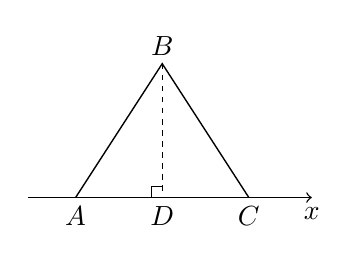
\begin{tikzpicture}[scale=1,line width=0.5pt]
\draw[->] (-0.4,0) -- (3.2,0) node[below] {$x$};
\draw (0.2,0) -- (1.3,1.7) -- (2.4,0);
\node at (0.2,-0.24) {$A$};
\node at (1.3,-0.24) {$D$};
\node at (2.4,-0.24) {$C$};
\node at (1.3,1.92) {$B$};
\draw[dash pattern=on 2pt off 2pt] (1.3,1.7) -- (1.3,0);
\draw (1.16,0) -- (1.16,0.14) -- (1.3,0.14);
\end{tikzpicture}
\end{center}
\step{$AB=AC=BC=\dfrac{2\sqrt3}3$，则 $x_2=x_1+AD=x_1+\dfrac{\sqrt3}3$，$x_3=x_1+\dfrac{2\sqrt3}3$，}
\step{存在 $x_1=-\dfrac{\sqrt3}3$，使得 $x_2=x_1+\dfrac{\sqrt3}3=0\in\Q$，且 $x_3=x_1+\dfrac{2\sqrt3}3=\dfrac{\sqrt3}3$ 为无理数，}
\step{即 $D(x_2)=1$，$D(x_3)=0$ 与图形一致，符合题意，}
\step{此时，$S_{\triangle ABC}=\dfrac12AC\cdot BD=\dfrac{\sqrt3}3$.}
\step{综上所述，存在这样的点 $A$、$B$、$C$，该正三角形的面积为 $\dfrac{\sqrt3}3$.}
\solend

\fi

\item 已知函数 $f(x)$ 满足：对 $\forall x\in R$，都有 $f(x+2025)\leqslant f(x)+2026$，
$f(x+2026)\geqslant f(x)+2027$，若 $f(1)=0$，则 $f(2)$ 的取值范围是\blankline[4.4em].

\ifanswer
\solbegin
\step{对 $\forall x\in R$，都有 $f(x+2025)\leqslant f(x)+2026$，$f(x+2026)\geqslant f(x)+2027$，}
\step{则 $f(x)+2027\leqslant f(x+2026)=f(x+1+2025)\leqslant f(x+1)+2026$，}
\step{即 $f(x)+1\leqslant f(x+1)$，所以 $f(2)\geqslant f(1)+1=1$；}
\step{$f(x)+2026\geqslant f(x+2025)=f(x+2024+1)\geqslant f(x+2024)+1$}
\step{$\geqslant\cdots\geqslant f(x+1)+2024$，所以 $f(x)+2\geqslant f(x+1)$，}
\step{所以 $f(2)\leqslant f(1)+2=2$；}
\step{即 $f(2)$ 的取值范围是 $[1,2]$.}
\solend

\fi

\end{enumerate}

\bigsec{二、选择题}

\begin{enumerate}
\setcounter{enumi}{12}

\item 若实数 $0<m<n<1$，而实数 $x>1$，则下列不等式正确的是\mbox{（\quad）}

\keepwithprev
A. $m^x<n^x$\qquad\qquad B. $x^m>x^n$\qquad\qquad C. $\log_xm>\log_xn$\qquad D. $\log_mx<\log_nx$

\ifanswer
\solbegin
\step{对于 $A$，函数 $f(t)=t^x$ 是以 $t$ 为变量，$x$ 为常量的幂函数，}
\step{由于 $x>1$，易得 $f(t)$ 在 $(0,+\infty)$ 上严格增，}
\step{$0<m<n<1$，$x>1$，可以得到 $m^x<n^x$，故 $A$ 正确；}
\step{对于 $B$，函数 $g(s)=x^s$，是以 $s$ 为变量，$x$ 为常量的指数函数，}
\step{由于 $x>1$，则 $g(s)$ 严格增，$0<m<n<1$，可以得到 $x^m<x^n$，故 $B$ 不正确；}
\step{对于 $C$，$\log_xm=\dfrac{\lg m}{\lg x}$，$\log_xn=\dfrac{\lg n}{\lg x}$，由于 $0<m<n<1$，则 $\lg m<\lg n<0$，}
\step{$x>1$，则 $\lg x>0$，则有 $\dfrac{\lg m}{\lg x}<\dfrac{\lg n}{\lg x}$，即 $\log_xm<\log_xn$，故 $C$ 不正确；}
\step{对于 $D$，由 $\log_mx-\log_nx=\dfrac{\lg x}{\lg m}-\dfrac{\lg x}{\lg n}=\dfrac{\lg x(\lg n-\lg m)}{\lg m\lg n}$，}
\step{因为实数 $0<m<n<1$，而实数 $x>1$，}
\step{所以 $\lg x>0$，$\lg m<\lg n<0$，则 $\dfrac{\lg x(\lg n-\lg m)}{\lg m\lg n}>0$，即 $\log_mx>\log_nx$，}
\step{故 $D$ 不正确.}
\step{故选 $A$.}
\solend

\fi

\item 已知 $x>1$，$y>1$，则 “$4^x>2^y$” 是 $\log_2x>\log_4(y-1)$ ”的\mbox{（\quad）}

\keepwithprev
A. 充分不必要条件\qquad\qquad B. 必要不充分条件

C. 充要条件\qquad\qquad D. 既不充分也不必要条件

\ifanswer
\solbegin
\step{因为 $x>1$，$y>1$，若 $4^x>2^y$，即 $2^{2x}>2^y$，所以 $2x>y>1$，}
\step{因为 $\dfrac y2-\sqrt{y-1}=\dfrac{(\sqrt{y-1})^2-2\sqrt{y-1}+1}2=\dfrac{(\sqrt{y-1}-1)^2}2\geqslant0$，}
\step{即 $\dfrac y2\geqslant\sqrt{y-1}>0$，所以 $\log_2\dfrac y2\geqslant\log_2\sqrt{y-1}=\dfrac12\log_2(y-1)=\log_4(y-1)$，}
\step{又 $x>\dfrac y2>\dfrac12$，所以 $\log_2x>\log_2\dfrac y2\geqslant\log_4(y-1)$，故充分性成立；}
\step{取 $x=2$，$y=4$，满足 $1=\log_2x>\log_4(y-1)=\log_43$，}
\step{但 $16=4^x=2^y=16$，即不满足 $4^x>2^y$，故必要性不成立.}% 链首链尾两个 16 系原卷笔误，应为 4^x=2^y=16，照录
\step{故选 $A$.}
\solend

\fi

\item 以下命题中，真命题的个数是\mbox{（\quad）}

①函数 $y=(x^2+1)^2+3$ 最小值为 3；②若 $2^a+\log_2a=4^b+2\log_4b$，则 $a<2b$；③不等式
$2^x-x-1>0$ 的解集为 $(1,+\infty)$.

\keepwithprev
A. $0$\qquad\qquad B. $1$\qquad\qquad C. $2$\qquad\qquad D. $3$

\ifanswer
\solbegin
\step{对于①，由于 $x^2+1\geqslant1$，则 $y=(x^2+1)^2+3\geqslant4$，}
\step{即函数 $y=(x^2+1)^2+3$ 最小值为 4，①错误；}
\step{对于②，由于 $b>0$，}
\step{则有 $2^a+\log_2a=4^b+2\log_4b=2^{2b}+\log_2b<2^{2b}+\log_22b$，}
\step{设 $f(x)=2^x+\log_2x$，易得 $f(x)$ 在 $(0,+\infty)$ 上为严格增函数，必有 $a<2b$，}
\step{②正确；}
\step{对于③，当 $x=-1$ 时，$2^x-x-1=2^x(x+1)>0$，即 $-1$ 在不等式的解集内，}
\step{③错误；}
\step{故选 $B$.}
\solend

\fi

\item 已知函数 $f(x)=ax^2+bx+c$（$a\neq0$ 且 $a<b$），若对任意的 $x\in R$，$f(x)\geqslant0$，且
$f(1)\geqslant\lambda(b-a)$，则实数 $\lambda$ 的取值范围为\mbox{（\quad）}

\keepwithprev
A. $(-\infty,2]$\qquad\qquad B. $[2\text{，}+\infty)$\qquad\qquad C. $(-\infty\text{，}3]$\qquad\qquad D. $[3\text{，}+\infty)$% 原卷 B/C/D 用全角逗号、A 用半角，照录

\ifanswer
\solbegin
\step{因为函数 $f(x)\geqslant0$ 恒成立，所以 $a>0$，且 $\Delta=b^2-4ac\leqslant0$，即 $c\geqslant\dfrac{b^2}{4a}$，}
\step{所以 $a+b+c\geqslant a+b+\dfrac{b^2}{4a}$，又 $a<b$，所以 $b-a>0$，}
\step{又 $f(1)\geqslant\lambda(b-a)$ 恒成立，所以 $a+b+c\geqslant\lambda(b-a)$ 恒成立，}
\step{即 $\lambda\leqslant\left(\dfrac{a+b+c}{b-a}\right)_{\min}=\dfrac{a+b+\dfrac{b^2}{4a}}{b-a}$，}
\step{令 $t=\dfrac ba$（$t>1$），则 $\dfrac{a+b+\dfrac{b^2}{4a}}{b-a}=\dfrac{1+t+\dfrac{t^2}4}{t-1}$，}
\step{令 $\mu=t-1$（$\mu>0$），则 $t=\mu+1$，}
\step{故上式 $=\dfrac{1+\mu+1+\dfrac{(\mu+1)^2}4}{\mu}=\dfrac14\left(\mu+\dfrac9\mu+6\right)$，}
\step{对 $\mu>0$，有 $\mu+\dfrac9\mu\geqslant2\sqrt{\mu\times\dfrac9\mu}=6$，当且仅当 $\mu=\dfrac9\mu$，即 $\mu=3$ 时取等号，}
\step{所以 $\dfrac14\left(\mu+\dfrac9\mu+6\right)\geqslant\dfrac14(6+6)=3$，故 $\lambda\leqslant3$，}
\step{即实数 $\lambda$ 的取值范围为 $(-\infty,3]$. 故选 $C$.}
\solend

\fi

\end{enumerate}

\bigsec{三、解答题}

\begin{enumerate}
\setcounter{enumi}{16}

\item 已知函数 $f(x)=\log_\frac23(ax^2-6x+18)$.

（1）若 $f(x)$ 的定义域为 $R$，求实数 $a$ 的取值范围.

（2）若 $f(x)$ 的值域为 $R$，求实数 $a$ 的取值范围.

\ansspace*[10]

\ifanswer
\solbegin
\stepm{（1）}{由 $f(x)=\log_\frac23(ax^2-6x+18)$ 的定义域为 $R$，得 $ax^2-6x+18>0$ 恒成立，}
\step{$a=0$ 时，$f(x)=\log_\frac23(18-6x)$ 的定义域为 $(-\infty,3)$，不符合题意.}
\step{$a\neq0$ 时，$\begin{cases}a>0\\ \Delta=36-4\times18a<0\end{cases}$，解得 $a>\dfrac12$.}
\step{综上，$a$ 的取值范围是 $\left(\dfrac12,+\infty\right)$.}
\stepm{（2）}{$a=0$ 时，$f(x)=\log_\frac23(18-6x)$ 的值域为 $R$，符合题意.}
\step{$a\neq0$ 时，$\begin{cases}a>0\\ \Delta=36-4\times18a\geqslant0\end{cases}$，解得 $0<a\leqslant\dfrac12$.}
\step{综上，$a$ 的取值范围是 $\left[0,\dfrac12\right]$.}
\solend

\fi

\item 已知 $f(x)=\log_ax+\log_a(6-x)$，$a>0$ 且 $a\neq1$，且 $f(3)=2$.

（1）求 $a$ 的值及 $f(x)$ 的单调区间.

（2）若对于 $\forall x_1\in(0,6)$，$\exists x_2\in[1,9]$，使得 $f(x_1)\leqslant t+\log_3x_2$ 成立，求实数 $t$ 的取值范
围.

\ansspace*[12]

\ifanswer
\solbegin
\stepm{（1）}{已知 $f(x)=\log_ax+\log_a(6-x)$，且 $f(3)=2$.}
\step{得 $\log_a3+\log_a(6-3)=2$，即 $2\log_a3=2$，}
\step{因此 $\log_a3=1$，因此 $a=3$，因此 $f(x)=\log_3x+\log_3(6-x)$，}
\step{因为 $\begin{cases}x>0\\ 6-x>0\end{cases}$，因此 $0<x<6$，故 $f(x)$ 的定义域为 $(0,6)$；}
\step{$f(x)=\log_3(6x-x^2)$，}
\step{因为函数 $y=6x-x^2$ 在 $(0,3)$ 上严格增，在 $(3,6)$ 上严格减，}
\step{又函数 $y=\log_3x$ 为严格增函数，}
\step{由复合函数的单调性得函数 $f(x)$ 在 $(0,3)$ 上严格增，在 $(3,6)$ 上严格减；}
\stepm{（2）}{令 $g(x)=t+\log_3x$，}
\step{因为 $\forall x_1\in(0,6)$，$\exists x_2\in[1,9]$，使得 $f(x_1)\leqslant t+\log_3x_2$，}
\step{即 $f(x_{1})_{\max}\leqslant g(x_{2})_{\max}$，}
\step{其中由（1）得 $f(x_{1})_{\max}=f(3)=2$.}
\step{又 $g(x)=t+\log_3x$ 在 $[1,9]$ 上严格增，因此 $g(x)_{\max}=g(9)=t+2$，}
\step{因此 $2\leqslant t+2$，因此实数 $t$ 的取值范围为 $[0,+\infty)$.}
\solend

\fi

\item 某心理学研究小组在对学生上课注意力集中情况的调查研究中，发现其注意力指数 $p$ 与
听课时间 $t$ 之间的关系满足如图所示的曲线. 当 $t\in(0,14]$ 时，曲线是二次函数图象的一部
分，当 $t\in[14,40]$ 时，曲线是函数 $y=\log_a(t-5)+83$（$a>0$ 且 $a\neq1$）图象的一部分. 根据
专家研究，当注意力指数 $p$ 大于等于 80 时听课效果最佳.

（1）试求 $p=f(t)$ 的函数关系式；

（2）当一位学生在坚持听课 32 分钟时，注意力指数 $p$ 大约为多少？

（3）一道数学难题，讲解需要 20 分钟，问老师能否经过合理安排在学生听
课效果最佳时讲完？请说明理由.

\begin{center}
% 原图第 9 页题干 p-t 曲线图按原图形状用 TikZ 重排（三版都出）。
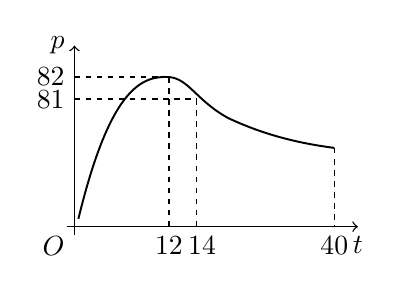
\begin{tikzpicture}[scale=1,line width=0.5pt]
\draw[->] (-0.1,0) -- (3.6,0) node[below] {$t$};
\draw[->] (0,-0.1) -- (0,2.3) node[left] {$p$};
\node[below left] at (0,0) {$O$};
\draw[line width=0.7pt] (0.05,0.1) .. controls (0.45,1.75) and (0.85,1.92) .. (1.2,1.9)
  .. controls (1.45,1.88) and (1.55,1.6) .. (1.95,1.38)
  .. controls (2.5,1.12) and (3.0,1.04) .. (3.3,1.0);
\draw[dash pattern=on 2pt off 2pt] (0,1.9) -- (1.2,1.9);
\draw[dash pattern=on 2pt off 2pt] (0,1.62) -- (1.55,1.62);
\draw[dash pattern=on 2pt off 2pt] (1.2,1.9) -- (1.2,0);
\draw[dash pattern=on 2pt off 2pt] (1.55,1.62) -- (1.55,0);
\draw[dash pattern=on 2pt off 2pt] (3.3,1.0) -- (3.3,0);
\node[left] at (0,1.9) {$82$};
\node[left] at (0,1.62) {$81$};
\node[below] at (1.2,0) {$12$};
\node[below] at (1.62,0) {$14$};
\node[below] at (3.3,0) {$40$};
\end{tikzpicture}
\end{center}

\ansspace*[12]

\ifanswer
\solbegin
\stepm{（1）}{由题意得当 $t\in(0,14]$ 时，设 $f(t)=c(t-12)^2+82$（$c<0$），}
\step{又 $f(14)=81$，所以 $c(14-12)^2+82=81$，解得 $c=-\dfrac14$；}
\step{所以 $f(t)=-\dfrac14(t-12)^2+82$,$t\in(0,14]$；}
\step{又当 $t\in[14,40]$ 时，函数 $y=\log_a(t-5)+83$（$a>0$ 且 $a\neq1$），}
\step{又当 $x=14$ 时，$y=81$，所以 $81=\log_a(14-5)+83$，解得 $a=\dfrac13$；}
\step{所以 $f(t)=\log_\frac13(t-5)+83$,$t\in[14,40]$，}
\step{所以 $p=\begin{cases}-\dfrac14(t-12)^2+82, & t\in(0,14]\\ \log_\frac13(t-5)+83, & t\in(14,40]\end{cases}$；}
\stepm{（2）}{当 $t=32$ 时，$p=\log_\frac13(32-5)+83=80$，}
\step{所以当一位学生在坚持听课 32 分钟时，注意力指数 $p$ 大约为 80；}
\stepm{（3）}{当 $t\in(0,14]$ 时，$-\dfrac14(t-12)^2+82\geqslant80$，解得 $t\in[12-2\sqrt2,14]$，}
\step{当 $t\in[14,40]$ 时，$\log_\frac13(t-5)+83\geqslant80$，解得 $5<t\leqslant32$，则 $t\in[14,32]$，}
\step{因此当 $t\in[12-2\sqrt2,32]$ 时学生听课效果最佳，}
\step{此时 $\Delta t=32-(12-2\sqrt2)=20+2\sqrt2>20$，}
\step{所以老师能经过合理安排时间在学生听课效果最佳时段讲完.}
\solend

\fi

\item 已知 $a\in R$，函数 $f(x+1)=\log_2\left(\dfrac{ax+1+a}{x+1}\right)$.

（1）若 $a=2$，求函数 $f(x)$ 的表达式及定义域；

（2）若关于 $x$ 的方程 $f\left(\dfrac x2\right)-\log_2[(a-2)x+3a-5]=0$ 的解集中恰好只有一个元素，求实
数 $a$ 的取值范围.

\ansspace*[14]

\ifanswer
\solbegin
\stepm{（1）}{$f(x+1)=\log_2\left(\dfrac{ax+1+a}{x+1}\right)$，}
\step{令 $x+1=t$，则 $f(t)=\log_2\left(\dfrac1t+a\right)$，即 $f(x)=\log_2\left(\dfrac1x+a\right)$，}
\step{因为 $a=2$，所以 $f(x)=\log_2\left(2+\dfrac1x\right)$，}
\step{由 $2+\dfrac1x>0$ 得定义域为 $\left(-\infty,-\dfrac12\right)\cup(0,+\infty)$；}
\stepm{（2）}{由（1）得 $f(x)=\log_2\left(\dfrac1x+a\right)$，}
\step{方程 $f\left(\dfrac x2\right)-\log_2[(a-2)x+3a-5]=0$，}
\step{即 $\log_2\left(\dfrac2x+a\right)-\log_2[(a-2)x+3a-5]=0$，}
\step{可转化为 $(a-2)x^2+(2a-5)x-2=0$，且 $\dfrac2x+a>0$.}
\step{①当 $a-2=0$，即 $a=2$ 时，$x=-2$，符合题意；}
\step{②当 $a-2\neq0$，即 $a\neq2$ 时，$x_1=-2$,$x_2=\dfrac1{a-2}$，}
\step{（$i$）当 $-2=\dfrac1{a-2}$ 时，即 $a=\dfrac32$ 时，符合题意；}
\step{（$ii$）当 $-2\neq\dfrac1{a-2}$ 时，即 $a\neq\dfrac32$ 且 $a\neq2$ 时，}
\step{要满足题意，则有 $\begin{cases}-1+a>0\\ 3a-4\leqslant0\end{cases}\Rightarrow1<a\leqslant\dfrac43$ 或 $\begin{cases}-1+a\leqslant0\\ 3a-4>0\end{cases}$，无解；}
\step{综上，$a$ 的取值范围 $\left(1,\dfrac43\right]\cup\left\{2,\dfrac32\right\}$.}
\solend

\fi

\item 已知函数 $y=f(x)$ 是定义在 $[0,+\infty)$ 上的函数，并且 $f(x)\geqslant0$，对于定义域内的任意自
变量的值 $x$、$y$，满足 $f(y)f(x^2f(y)+xf(y))=f(x^2+y+x)$，$f(a)=0$，其中
$a>0$.

（1）当 $f(0)\neq0$ 时，求 $f(0)$；

（2）已知当 $0\leqslant x<a$ 时，有 $f(x)\neq0$.

（$i$）求 $f(a+3)$；

（$ii$）求函数 $y=f(x)$ 的解析式（用 $a$ 表示）.

\ansspace*[16]

\ifanswer
\solbegin
\stepm{（1）}{因为 $f(x)\geqslant0$，且对于定义域内的任意自变量的值 $x$、$y$，}
\step{满足 $f(y)f(x^2f(y)+xf(y))=f(x^2+y+x)$，}
\step{令 $x=y=0$，则 $f^2(0)=f(0)$，因为 $f(0)\neq0$，所以 $f(0)=1$，}
\stepm{（2）}{（$i$）由 $f(y)f(x^2f(y)+xf(y))=f(x^2+y+x)$，}
\step{得 $f(y)f[(x^2+x)f(y)]=f[(x^2+x)+y]$，}
\step{令 $t=x^2+x$，因为 $x\geqslant0$，所以 $t=x^2+x\in[0,+\infty)$，}
\step{所以有 $f(y)f(tf(y))=f(t+y)$，因为 $f(a)=0$，}
\step{令 $y=a$，$t=3$，得 $f(a+3)=f(a)f(3f(a))=0\times f(3f(a))=0$；}
\step{（$ii$）当 $x\geqslant a$ 时，令 $y=a$，$t=x-a$，}
\step{$f(x)=f(x-a+a)=f(a)f[(x-a)f(a)]=0$.}
\step{当 $0\leqslant x<a$ 时，则有 $0<a-x\leqslant a$，令 $y=x$，$t=a-x$，}
\step{则 $f(a)=f(a-x+x)=f(x)f[(a-x)f(x)]=0$.}
\step{因为 $f(x)\neq0$，所以有 $f((a-x)f(x))=0$，则 $(a-x)f(x)\geqslant a$，}
\step{又因为 $a-x>0$，即 $f(x)\geqslant\dfrac a{a-x}$.}
\step{令 $t=\dfrac a{f(x)}>0$,$y=x>0$，}
\step{则 $f\left(\dfrac a{f(x)}+x\right)=f(x)\cdot f\left(\dfrac a{f(x)}\cdot f(x)\right)=f(x)\cdot f(a)=0$，}
\step{所以有 $\dfrac a{f(x)}+x\geqslant a$，即 $\dfrac a{f(x)}\geqslant a-x$，得 $f(x)\leqslant\dfrac a{a-x}$，}
\step{所以当 $0\leqslant x<a$ 时，$f(x)=\dfrac a{a-x}$.}
\step{综上，$f(x)=\begin{cases}\dfrac a{a-x}, & 0\leqslant x<a\\ 0, & x\geqslant a\end{cases}$.}
\solend

\fi

\end{enumerate}

\end{document}
"
%
% 原始材料：微信公众号“魔都数学加油站”文章，作者破晓，2026-11-02 17:41 发布；
% 连载“27学年高一105”，原文标题“27学年高一105——2026-2027年上海市交附闵行高一上周末作业10.30”；
% 原文链接：https://mp.weixin.qq.com/s/XUfNEvGHjD0CB5jdoleBWw。
% 正文为 13 张 PNG 页（第 4、9、13 页 2560×3620，其余 4762×6735），题目下印有【解析】，为讲评版。
% 题目、解析均据原图转录；卷面水印及公众号页脚未录入。
%
% 卷首标题：原卷印作“2026-2027 年交附闵行高一上周末作业 10.30”（公众号标题中的“上海市”
% 卷面标题行没有，本稿照卷面），年份区间按全稿惯例排 en dash；原卷未印副标题，本稿按题目
% 内容标为“函数、不等式”（主体为指数与对数，第 3 题集合、第 16 题基本不等式）。
%
% 与原卷的排版差异：
%   ① 原文从第 3 题起，填空题编号为 3—12、选择题为 13—16、解答题为 17—21，本稿保留原题号；
%   ② 原卷每题下直接印【解析】，本稿按全稿惯例将解析置于答案版；选择题括号内未印答案，另由
%      解析末句“故选 X”给出；
%   ③ 原卷未印副标题，本稿按“知识模块”口径补出；
%   ④ 原卷填空横线按全稿惯例排为 \blankline[4.4em]；解答题按惯例加 \ansspace；选择题括号排
%      \mbox{（\quad）}、选项段前按惯例加 \keepwithprev；
%   ⑤ $f(x_1)_{max}$、$g(x)_max$、$\left(\frac{a+b+c}{b-a}\right)_{min}$ 等下标原卷排斜体，
%      按 高一96 成例改正体 $\max$、$\min$；
%   ⑥ 原卷数集排斜体 $R$／$Q$，按全稿惯例改 $\R$／$\Q$；
%   ⑦ 第 11 题解析的两幅三角形示意图与第 19 题题干的 $p$-$t$ 曲线图均按原图形状用 TikZ 重排
%      （第 19 题图属题干、三版都出；第 11 题图属解析、仅答案版显示）。
%
% 原卷存疑／笔误（均照录加注）：
%   第 14 题解析“但 $16=4^x=2^y=16$”（链首、链尾的两个 $16$ 系原卷笔误，按上下文应为
%   $4^x=2^y=16$）；
%   第 16 题选项的区间分隔逗号 A 项排半角、B／C／D 三项排全角（原卷自身不一致）；
%   第 21 题 (2) 的小问号排“（$i$）求…”（右括号紧贴“求”字），照录。
%
% 行数核对：逐题数 \step/\stepm 条数，合计 159 条（Q3：2；Q4：1；Q5：4；Q6：6；Q7：3；
% Q8：7；Q9：5；Q10：3；Q11：15；Q12：7；Q13：12；Q14：7；Q15：9；Q16：10；Q17：7；
% Q18：14；Q19：14；Q20：14；Q21：19），与原卷印刷行逐题相等。
%
\documentclass[a4paper,11pt]{article}
\usepackage{common}

\begin{document}

\examtitlest[3]{2026--2027 年交附闵行高一上周末作业 10.30}{函数、不等式}

\bigsec{一、填空题}

\begin{enumerate}
\setcounter{enumi}{2}

\item 已知集合 $M=\{1,m\}$，$N=\{n,\log_2n\}$，若 $M=N$，则 $(m-n)^{2027}=$\blankline[4.4em].

\ifanswer
\solbegin
\step{由题意得 $\begin{cases}n=1\\ \log_2n=m\end{cases}$ 或 $\begin{cases}n=m\\ \log_2n=1\end{cases}$，解得 $\begin{cases}n=1\\ m=0\end{cases}$ 或 $\begin{cases}n=2\\ m=2\end{cases}$，}
\step{所以 $(m-n)^{2027}=-1$ 或 $0$.}
\solend

\fi

\item 已知 $\log_{2x^2-1}(3x^2+2x-1)=1$，则 $x=$\blankline[4.4em].

\ifanswer
\solbegin
\step{因为 $\log_{2x^2-1}(3x^2+2x-1)=1$，所以 $\begin{cases}2x^2-1>0\\ 2x^2-1\neq1\\ 3x^2+2x-1>0\\ 2x^2-1=3x^2+2x-1\end{cases}$，解得 $x=-2$.}
\solend

\fi

\item 已知 $m>1$，$n>1$，$\lg m=\log_n100$，则 $mn$ 的最小值为\blankline[4.4em].

\ifanswer
\solbegin
\step{由 $m>1$，$n>1$，得 $\lg m>0$，$\lg n>0$，}
\step{因为 $\lg m=\log_n100=\dfrac{\lg100}{\lg n}=\dfrac2{\lg n}$，所以 $\lg m\cdot\lg n=2$，}
\step{所以 $\lg(mn)=\lg m+\lg n\geqslant2\sqrt{\lg m\cdot\lg n}=2\sqrt2$，}
\step{当且仅当 $m=n=10^{\sqrt2}$ 时取等号，则 $mn\geqslant10^{2\sqrt2}$，即 $mn$ 的最小值为 $10^{2\sqrt2}$.}
\solend

\fi

\item 设 $m$、$n$ 分别是方程 $\log_{2013}x+x-9=0$ 和 $2013^x+x-9=0$ 的根，则 $m+n=$\blankline[4.4em].

\ifanswer
\solbegin
\step{由 $\log_{2013}x+x-9=0$，得 $\log_{2013}x=-x+9$，}
\step{因为 $m$ 是方程 $\log_{2013}x+x-9=0$ 的根，}
\step{所以 $m$ 为函数 $y=\log_{2013}x$ 与 $y=-x+9$ 图象交点的横坐标，}
\step{同理 $n$ 是函数 $y=2013^x$ 与 $y=-x+9$ 图象交点的横坐标，}
\step{因为 $y=\log_{2013}x$ 与 $y=2013^x$ 互为反函数，其图象关于直线 $y=x$ 对称，}
\step{联立 $\begin{cases}y=-x+9\\ y=x\end{cases}$，解得 $x=\dfrac92$，所以 $m+n=\dfrac92\times2=9$.}
\solend

\fi

\item 已知函数 $f(x)=\dfrac1{\log_2(x^2+4)}$，则 $f(-2)=$\blankline[2em]，$f(x)$ 的值域为\blankline[4.4em].

\ifanswer
\solbegin
\step{$f(-2)=\dfrac1{\log_28}=\dfrac13$.}
\step{因为 $x^2+4\geqslant4$，所以 $\log_2(x^2+4)\geqslant\log_24=2$，所以 $0<\dfrac1{\log_2(x^2+4)}\leqslant\dfrac12$，}
\step{故 $f(x)$ 的值域为 $\left(0,\dfrac12\right]$.}
\solend

\fi

\item 已知 $\alpha$、$\beta$ 是方程 $9^x-2m\cdot3^x+m^2-1=0$ 的两个根，若 $\alpha+\beta=1$，则 $\alpha\beta=$\blankline[4.4em].

\ifanswer
\solbegin
\step{由题意得方程 $9^x-2m\cdot3^x+m^2-1=0$ 有两个根，}
\step{则方程 $t^2-2mt+m^2-1=0$ 有二正根，}
\step{则 $\begin{cases}\Delta=4m^2-4(m^2-1)\geqslant0\\ 2m>0\\ m^2-1>0\end{cases}$，解得 $m>1$，}
\step{又 $\alpha$、$\beta$ 是方程 $9^x-2m\cdot3^x+m^2-1=0$ 的两个根，}
\step{则 $3^\alpha\times3^\beta=m^2-1$，又 $\alpha+\beta=1$，则 $m^2-1=3^{\alpha+\beta}=3$，}
\step{解得 $m=2$ 或 $m=-2$（舍），则 $3^\alpha+3^\beta=2m=4$，又 $\alpha=1-\beta$，}
\step{则 $3^{1-\beta}+3^\beta=4$，解得 $\beta=0$ 或 $\beta=1$，则 $\begin{cases}\alpha=1\\ \beta=0\end{cases}$ 或 $\begin{cases}\alpha=0\\ \beta=1\end{cases}$，则 $\alpha\beta=0$.}
\solend

\fi

\item 已知 $a>b>0$，$\ln a=2\ln b$，且 $a\lg b=b\lg a$，则 $a+b=$\blankline[4.4em].

\ifanswer
\solbegin
\step{因为 $a>b>0$，$\ln a=2\ln b=\ln b^2$，所以 $a=b^2$，}
\step{由 $a\lg b=b\lg a$ 得 $b^2\lg b=b\lg b^2$，即 $b\lg b=2\lg b$，所以 $b=1$ 或 $b=2$，}
\step{当 $b=2$，$a=4$，满足题意，}
\step{当 $b=1$ 时，$a=1$ 与 $a>b>0$ 矛盾，所以 $b=1$ 舍去，}
\step{所以 $a+b=6$.}
\solend

\fi

\item 函数 $f(x)=\begin{cases}2^x, & x\leqslant t\\ \log_\frac12x, & x>t\end{cases}$ 的值域为 $M$，且 $8\notin M$，则实数 $t$ 的取值集合为\blankline[4.4em].

\ifanswer
\solbegin
\step{当 $x\leqslant t$ 时，函数 $f(x)=2^x$ 在 $(-\infty,t]$ 严格增，}
\step{当 $x>t$ 时，$f(x)=\log_\frac12x$ 在 $(t,+\infty)$ 严格减，}
\step{若 $8\notin M$，则满足条件 $\begin{cases}2^t<8\\ \log_\frac12t\leqslant8\end{cases}\Rightarrow\dfrac1{256}\leqslant t<3$，故实数 $t$ 的取值集合为 $\left[\dfrac1{256},3\right)$.}
\solend

\fi

\item 德国数学家狄利克雷在数学领域成就显著，以其命名函数 $D(x)=\begin{cases}1, & x\text{为有理数}\\ 0, & x\text{为无理数}\end{cases}$，该函
数被称为狄利克雷函数。那么是否存在三个点 $A(x_1,D(x_1))$、$B(x_2,D(x_2))$、$C(x_3,D(x_3))$，
使得 $\triangle ABC$ 为等边三角形，若不存在请在横线上填写“不存在”，如果存在则在横线上填写
该正三角形的面积\blankline[4.4em].

\ifanswer
\solbegin
\step{因为 $D(x)=\begin{cases}1, & x\text{为有理数}\\ 0, & x\text{为无理数}\end{cases}$，所以 $D(x)=0$ 或 1，}
\step{设存在三个点 $A(x_1,D(x_1))$、$B(x_2,D(x_2))$、$C(x_3,D(x_3))$，}
\step{使得 $\triangle ABC$ 为等边三角形，则 $D(x_1)$、$D(x_2)$、$D(x_3)$ 不同时为 0 或 1，}
\step{不妨设 $x_1<x_2<x_3$，分析得 $\triangle ABC$ 的位置有两种情况，}
\step{第一种情况：当 $x_1$ 为有理数时，即 $D(x_1)=1$，如图，过点 $B$ 作 $BD\perp AC$，}
\begin{center}
% 原图第 4 页解析示意图按原图形状用 TikZ 重排（第一种情况：$B$ 在 $x$ 轴上、$AC$ 在上方）。
\begin{tikzpicture}[scale=1,line width=0.5pt]
\draw (0,1.2) -- (2.6,1.2);
\node at (0.25,1.4) {$A$};
\node at (1.3,1.4) {$D$};
\node at (2.35,1.4) {$C$};
\draw[dash pattern=on 2pt off 2pt] (1.3,1.2) -- (1.3,0);
\draw (1.16,1.2) -- (1.16,1.06) -- (1.3,1.06);
\draw[->] (-0.5,0) -- (3.1,0) node[below] {$x$};
\node at (1.3,-0.24) {$B$};
\end{tikzpicture}
\end{center}
\step{垂足为 $D$，得 $BD=1$，$AD=\dfrac{\sqrt3}3$，$AB=AC=BC=\dfrac{2\sqrt3}3$，}
\step{则 $x_2=x_1+AD=x_1+\dfrac{\sqrt3}3$ 为无理数，$x_3=x_1+\dfrac{2\sqrt3}3$ 为无理数，}
\step{即 $D(x_2)=0$，$D(x_3)=0$ 与图形不一致，舍去；}
\step{第二种情况：当 $x_1$ 为无理数时，即 $D(x_1)=0$，如图，}
\step{过点 $B$ 作 $BD\perp AC$，垂足为 $D$，得 $BD=1$，$AD=\dfrac{\sqrt3}3$，}
\begin{center}
% 原图第 4 页解析示意图按原图形状用 TikZ 重排（第二种情况：$B$ 在上方、$AC$ 在 $x$ 轴上）。
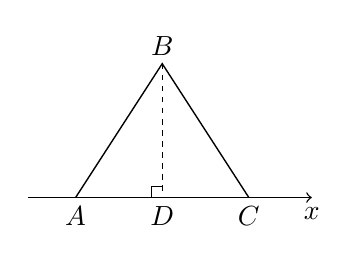
\begin{tikzpicture}[scale=1,line width=0.5pt]
\draw[->] (-0.4,0) -- (3.2,0) node[below] {$x$};
\draw (0.2,0) -- (1.3,1.7) -- (2.4,0);
\node at (0.2,-0.24) {$A$};
\node at (1.3,-0.24) {$D$};
\node at (2.4,-0.24) {$C$};
\node at (1.3,1.92) {$B$};
\draw[dash pattern=on 2pt off 2pt] (1.3,1.7) -- (1.3,0);
\draw (1.16,0) -- (1.16,0.14) -- (1.3,0.14);
\end{tikzpicture}
\end{center}
\step{$AB=AC=BC=\dfrac{2\sqrt3}3$，则 $x_2=x_1+AD=x_1+\dfrac{\sqrt3}3$，$x_3=x_1+\dfrac{2\sqrt3}3$，}
\step{存在 $x_1=-\dfrac{\sqrt3}3$，使得 $x_2=x_1+\dfrac{\sqrt3}3=0\in\Q$，且 $x_3=x_1+\dfrac{2\sqrt3}3=\dfrac{\sqrt3}3$ 为无理数，}
\step{即 $D(x_2)=1$，$D(x_3)=0$ 与图形一致，符合题意，}
\step{此时，$S_{\triangle ABC}=\dfrac12AC\cdot BD=\dfrac{\sqrt3}3$.}
\step{综上所述，存在这样的点 $A$、$B$、$C$，该正三角形的面积为 $\dfrac{\sqrt3}3$.}
\solend

\fi

\item 已知函数 $f(x)$ 满足：对 $\forall x\in R$，都有 $f(x+2025)\leqslant f(x)+2026$，
$f(x+2026)\geqslant f(x)+2027$，若 $f(1)=0$，则 $f(2)$ 的取值范围是\blankline[4.4em].

\ifanswer
\solbegin
\step{对 $\forall x\in R$，都有 $f(x+2025)\leqslant f(x)+2026$，$f(x+2026)\geqslant f(x)+2027$，}
\step{则 $f(x)+2027\leqslant f(x+2026)=f(x+1+2025)\leqslant f(x+1)+2026$，}
\step{即 $f(x)+1\leqslant f(x+1)$，所以 $f(2)\geqslant f(1)+1=1$；}
\step{$f(x)+2026\geqslant f(x+2025)=f(x+2024+1)\geqslant f(x+2024)+1$}
\step{$\geqslant\cdots\geqslant f(x+1)+2024$，所以 $f(x)+2\geqslant f(x+1)$，}
\step{所以 $f(2)\leqslant f(1)+2=2$；}
\step{即 $f(2)$ 的取值范围是 $[1,2]$.}
\solend

\fi

\end{enumerate}

\bigsec{二、选择题}

\begin{enumerate}
\setcounter{enumi}{12}

\item 若实数 $0<m<n<1$，而实数 $x>1$，则下列不等式正确的是\mbox{（\quad）}

\keepwithprev
A. $m^x<n^x$\qquad\qquad B. $x^m>x^n$\qquad\qquad C. $\log_xm>\log_xn$\qquad D. $\log_mx<\log_nx$

\ifanswer
\solbegin
\step{对于 $A$，函数 $f(t)=t^x$ 是以 $t$ 为变量，$x$ 为常量的幂函数，}
\step{由于 $x>1$，易得 $f(t)$ 在 $(0,+\infty)$ 上严格增，}
\step{$0<m<n<1$，$x>1$，可以得到 $m^x<n^x$，故 $A$ 正确；}
\step{对于 $B$，函数 $g(s)=x^s$，是以 $s$ 为变量，$x$ 为常量的指数函数，}
\step{由于 $x>1$，则 $g(s)$ 严格增，$0<m<n<1$，可以得到 $x^m<x^n$，故 $B$ 不正确；}
\step{对于 $C$，$\log_xm=\dfrac{\lg m}{\lg x}$，$\log_xn=\dfrac{\lg n}{\lg x}$，由于 $0<m<n<1$，则 $\lg m<\lg n<0$，}
\step{$x>1$，则 $\lg x>0$，则有 $\dfrac{\lg m}{\lg x}<\dfrac{\lg n}{\lg x}$，即 $\log_xm<\log_xn$，故 $C$ 不正确；}
\step{对于 $D$，由 $\log_mx-\log_nx=\dfrac{\lg x}{\lg m}-\dfrac{\lg x}{\lg n}=\dfrac{\lg x(\lg n-\lg m)}{\lg m\lg n}$，}
\step{因为实数 $0<m<n<1$，而实数 $x>1$，}
\step{所以 $\lg x>0$，$\lg m<\lg n<0$，则 $\dfrac{\lg x(\lg n-\lg m)}{\lg m\lg n}>0$，即 $\log_mx>\log_nx$，}
\step{故 $D$ 不正确.}
\step{故选 $A$.}
\solend

\fi

\item 已知 $x>1$，$y>1$，则 “$4^x>2^y$” 是 $\log_2x>\log_4(y-1)$ ”的\mbox{（\quad）}

\keepwithprev
A. 充分不必要条件\qquad\qquad B. 必要不充分条件

C. 充要条件\qquad\qquad D. 既不充分也不必要条件

\ifanswer
\solbegin
\step{因为 $x>1$，$y>1$，若 $4^x>2^y$，即 $2^{2x}>2^y$，所以 $2x>y>1$，}
\step{因为 $\dfrac y2-\sqrt{y-1}=\dfrac{(\sqrt{y-1})^2-2\sqrt{y-1}+1}2=\dfrac{(\sqrt{y-1}-1)^2}2\geqslant0$，}
\step{即 $\dfrac y2\geqslant\sqrt{y-1}>0$，所以 $\log_2\dfrac y2\geqslant\log_2\sqrt{y-1}=\dfrac12\log_2(y-1)=\log_4(y-1)$，}
\step{又 $x>\dfrac y2>\dfrac12$，所以 $\log_2x>\log_2\dfrac y2\geqslant\log_4(y-1)$，故充分性成立；}
\step{取 $x=2$，$y=4$，满足 $1=\log_2x>\log_4(y-1)=\log_43$，}
\step{但 $16=4^x=2^y=16$，即不满足 $4^x>2^y$，故必要性不成立.}% 链首链尾两个 16 系原卷笔误，应为 4^x=2^y=16，照录
\step{故选 $A$.}
\solend

\fi

\item 以下命题中，真命题的个数是\mbox{（\quad）}

①函数 $y=(x^2+1)^2+3$ 最小值为 3；②若 $2^a+\log_2a=4^b+2\log_4b$，则 $a<2b$；③不等式
$2^x-x-1>0$ 的解集为 $(1,+\infty)$.

\keepwithprev
A. $0$\qquad\qquad B. $1$\qquad\qquad C. $2$\qquad\qquad D. $3$

\ifanswer
\solbegin
\step{对于①，由于 $x^2+1\geqslant1$，则 $y=(x^2+1)^2+3\geqslant4$，}
\step{即函数 $y=(x^2+1)^2+3$ 最小值为 4，①错误；}
\step{对于②，由于 $b>0$，}
\step{则有 $2^a+\log_2a=4^b+2\log_4b=2^{2b}+\log_2b<2^{2b}+\log_22b$，}
\step{设 $f(x)=2^x+\log_2x$，易得 $f(x)$ 在 $(0,+\infty)$ 上为严格增函数，必有 $a<2b$，}
\step{②正确；}
\step{对于③，当 $x=-1$ 时，$2^x-x-1=2^x(x+1)>0$，即 $-1$ 在不等式的解集内，}
\step{③错误；}
\step{故选 $B$.}
\solend

\fi

\item 已知函数 $f(x)=ax^2+bx+c$（$a\neq0$ 且 $a<b$），若对任意的 $x\in R$，$f(x)\geqslant0$，且
$f(1)\geqslant\lambda(b-a)$，则实数 $\lambda$ 的取值范围为\mbox{（\quad）}

\keepwithprev
A. $(-\infty,2]$\qquad\qquad B. $[2\text{，}+\infty)$\qquad\qquad C. $(-\infty\text{，}3]$\qquad\qquad D. $[3\text{，}+\infty)$% 原卷 B/C/D 用全角逗号、A 用半角，照录

\ifanswer
\solbegin
\step{因为函数 $f(x)\geqslant0$ 恒成立，所以 $a>0$，且 $\Delta=b^2-4ac\leqslant0$，即 $c\geqslant\dfrac{b^2}{4a}$，}
\step{所以 $a+b+c\geqslant a+b+\dfrac{b^2}{4a}$，又 $a<b$，所以 $b-a>0$，}
\step{又 $f(1)\geqslant\lambda(b-a)$ 恒成立，所以 $a+b+c\geqslant\lambda(b-a)$ 恒成立，}
\step{即 $\lambda\leqslant\left(\dfrac{a+b+c}{b-a}\right)_{\min}=\dfrac{a+b+\dfrac{b^2}{4a}}{b-a}$，}
\step{令 $t=\dfrac ba$（$t>1$），则 $\dfrac{a+b+\dfrac{b^2}{4a}}{b-a}=\dfrac{1+t+\dfrac{t^2}4}{t-1}$，}
\step{令 $\mu=t-1$（$\mu>0$），则 $t=\mu+1$，}
\step{故上式 $=\dfrac{1+\mu+1+\dfrac{(\mu+1)^2}4}{\mu}=\dfrac14\left(\mu+\dfrac9\mu+6\right)$，}
\step{对 $\mu>0$，有 $\mu+\dfrac9\mu\geqslant2\sqrt{\mu\times\dfrac9\mu}=6$，当且仅当 $\mu=\dfrac9\mu$，即 $\mu=3$ 时取等号，}
\step{所以 $\dfrac14\left(\mu+\dfrac9\mu+6\right)\geqslant\dfrac14(6+6)=3$，故 $\lambda\leqslant3$，}
\step{即实数 $\lambda$ 的取值范围为 $(-\infty,3]$. 故选 $C$.}
\solend

\fi

\end{enumerate}

\bigsec{三、解答题}

\begin{enumerate}
\setcounter{enumi}{16}

\item 已知函数 $f(x)=\log_\frac23(ax^2-6x+18)$.

（1）若 $f(x)$ 的定义域为 $R$，求实数 $a$ 的取值范围.

（2）若 $f(x)$ 的值域为 $R$，求实数 $a$ 的取值范围.

\ansspace*[10]

\ifanswer
\solbegin
\stepm{（1）}{由 $f(x)=\log_\frac23(ax^2-6x+18)$ 的定义域为 $R$，得 $ax^2-6x+18>0$ 恒成立，}
\step{$a=0$ 时，$f(x)=\log_\frac23(18-6x)$ 的定义域为 $(-\infty,3)$，不符合题意.}
\step{$a\neq0$ 时，$\begin{cases}a>0\\ \Delta=36-4\times18a<0\end{cases}$，解得 $a>\dfrac12$.}
\step{综上，$a$ 的取值范围是 $\left(\dfrac12,+\infty\right)$.}
\stepm{（2）}{$a=0$ 时，$f(x)=\log_\frac23(18-6x)$ 的值域为 $R$，符合题意.}
\step{$a\neq0$ 时，$\begin{cases}a>0\\ \Delta=36-4\times18a\geqslant0\end{cases}$，解得 $0<a\leqslant\dfrac12$.}
\step{综上，$a$ 的取值范围是 $\left[0,\dfrac12\right]$.}
\solend

\fi

\item 已知 $f(x)=\log_ax+\log_a(6-x)$，$a>0$ 且 $a\neq1$，且 $f(3)=2$.

（1）求 $a$ 的值及 $f(x)$ 的单调区间.

（2）若对于 $\forall x_1\in(0,6)$，$\exists x_2\in[1,9]$，使得 $f(x_1)\leqslant t+\log_3x_2$ 成立，求实数 $t$ 的取值范
围.

\ansspace*[12]

\ifanswer
\solbegin
\stepm{（1）}{已知 $f(x)=\log_ax+\log_a(6-x)$，且 $f(3)=2$.}
\step{得 $\log_a3+\log_a(6-3)=2$，即 $2\log_a3=2$，}
\step{因此 $\log_a3=1$，因此 $a=3$，因此 $f(x)=\log_3x+\log_3(6-x)$，}
\step{因为 $\begin{cases}x>0\\ 6-x>0\end{cases}$，因此 $0<x<6$，故 $f(x)$ 的定义域为 $(0,6)$；}
\step{$f(x)=\log_3(6x-x^2)$，}
\step{因为函数 $y=6x-x^2$ 在 $(0,3)$ 上严格增，在 $(3,6)$ 上严格减，}
\step{又函数 $y=\log_3x$ 为严格增函数，}
\step{由复合函数的单调性得函数 $f(x)$ 在 $(0,3)$ 上严格增，在 $(3,6)$ 上严格减；}
\stepm{（2）}{令 $g(x)=t+\log_3x$，}
\step{因为 $\forall x_1\in(0,6)$，$\exists x_2\in[1,9]$，使得 $f(x_1)\leqslant t+\log_3x_2$，}
\step{即 $f(x_{1})_{\max}\leqslant g(x_{2})_{\max}$，}
\step{其中由（1）得 $f(x_{1})_{\max}=f(3)=2$.}
\step{又 $g(x)=t+\log_3x$ 在 $[1,9]$ 上严格增，因此 $g(x)_{\max}=g(9)=t+2$，}
\step{因此 $2\leqslant t+2$，因此实数 $t$ 的取值范围为 $[0,+\infty)$.}
\solend

\fi

\item 某心理学研究小组在对学生上课注意力集中情况的调查研究中，发现其注意力指数 $p$ 与
听课时间 $t$ 之间的关系满足如图所示的曲线. 当 $t\in(0,14]$ 时，曲线是二次函数图象的一部
分，当 $t\in[14,40]$ 时，曲线是函数 $y=\log_a(t-5)+83$（$a>0$ 且 $a\neq1$）图象的一部分. 根据
专家研究，当注意力指数 $p$ 大于等于 80 时听课效果最佳.

（1）试求 $p=f(t)$ 的函数关系式；

（2）当一位学生在坚持听课 32 分钟时，注意力指数 $p$ 大约为多少？

（3）一道数学难题，讲解需要 20 分钟，问老师能否经过合理安排在学生听
课效果最佳时讲完？请说明理由.

\begin{center}
% 原图第 9 页题干 p-t 曲线图按原图形状用 TikZ 重排（三版都出）。
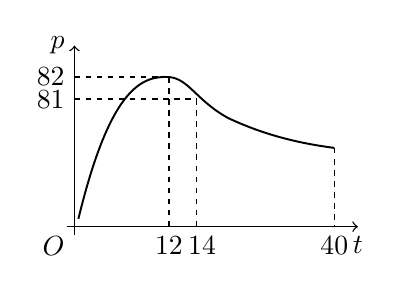
\begin{tikzpicture}[scale=1,line width=0.5pt]
\draw[->] (-0.1,0) -- (3.6,0) node[below] {$t$};
\draw[->] (0,-0.1) -- (0,2.3) node[left] {$p$};
\node[below left] at (0,0) {$O$};
\draw[line width=0.7pt] (0.05,0.1) .. controls (0.45,1.75) and (0.85,1.92) .. (1.2,1.9)
  .. controls (1.45,1.88) and (1.55,1.6) .. (1.95,1.38)
  .. controls (2.5,1.12) and (3.0,1.04) .. (3.3,1.0);
\draw[dash pattern=on 2pt off 2pt] (0,1.9) -- (1.2,1.9);
\draw[dash pattern=on 2pt off 2pt] (0,1.62) -- (1.55,1.62);
\draw[dash pattern=on 2pt off 2pt] (1.2,1.9) -- (1.2,0);
\draw[dash pattern=on 2pt off 2pt] (1.55,1.62) -- (1.55,0);
\draw[dash pattern=on 2pt off 2pt] (3.3,1.0) -- (3.3,0);
\node[left] at (0,1.9) {$82$};
\node[left] at (0,1.62) {$81$};
\node[below] at (1.2,0) {$12$};
\node[below] at (1.62,0) {$14$};
\node[below] at (3.3,0) {$40$};
\end{tikzpicture}
\end{center}

\ansspace*[12]

\ifanswer
\solbegin
\stepm{（1）}{由题意得当 $t\in(0,14]$ 时，设 $f(t)=c(t-12)^2+82$（$c<0$），}
\step{又 $f(14)=81$，所以 $c(14-12)^2+82=81$，解得 $c=-\dfrac14$；}
\step{所以 $f(t)=-\dfrac14(t-12)^2+82$,$t\in(0,14]$；}
\step{又当 $t\in[14,40]$ 时，函数 $y=\log_a(t-5)+83$（$a>0$ 且 $a\neq1$），}
\step{又当 $x=14$ 时，$y=81$，所以 $81=\log_a(14-5)+83$，解得 $a=\dfrac13$；}
\step{所以 $f(t)=\log_\frac13(t-5)+83$,$t\in[14,40]$，}
\step{所以 $p=\begin{cases}-\dfrac14(t-12)^2+82, & t\in(0,14]\\ \log_\frac13(t-5)+83, & t\in(14,40]\end{cases}$；}
\stepm{（2）}{当 $t=32$ 时，$p=\log_\frac13(32-5)+83=80$，}
\step{所以当一位学生在坚持听课 32 分钟时，注意力指数 $p$ 大约为 80；}
\stepm{（3）}{当 $t\in(0,14]$ 时，$-\dfrac14(t-12)^2+82\geqslant80$，解得 $t\in[12-2\sqrt2,14]$，}
\step{当 $t\in[14,40]$ 时，$\log_\frac13(t-5)+83\geqslant80$，解得 $5<t\leqslant32$，则 $t\in[14,32]$，}
\step{因此当 $t\in[12-2\sqrt2,32]$ 时学生听课效果最佳，}
\step{此时 $\Delta t=32-(12-2\sqrt2)=20+2\sqrt2>20$，}
\step{所以老师能经过合理安排时间在学生听课效果最佳时段讲完.}
\solend

\fi

\item 已知 $a\in R$，函数 $f(x+1)=\log_2\left(\dfrac{ax+1+a}{x+1}\right)$.

（1）若 $a=2$，求函数 $f(x)$ 的表达式及定义域；

（2）若关于 $x$ 的方程 $f\left(\dfrac x2\right)-\log_2[(a-2)x+3a-5]=0$ 的解集中恰好只有一个元素，求实
数 $a$ 的取值范围.

\ansspace*[14]

\ifanswer
\solbegin
\stepm{（1）}{$f(x+1)=\log_2\left(\dfrac{ax+1+a}{x+1}\right)$，}
\step{令 $x+1=t$，则 $f(t)=\log_2\left(\dfrac1t+a\right)$，即 $f(x)=\log_2\left(\dfrac1x+a\right)$，}
\step{因为 $a=2$，所以 $f(x)=\log_2\left(2+\dfrac1x\right)$，}
\step{由 $2+\dfrac1x>0$ 得定义域为 $\left(-\infty,-\dfrac12\right)\cup(0,+\infty)$；}
\stepm{（2）}{由（1）得 $f(x)=\log_2\left(\dfrac1x+a\right)$，}
\step{方程 $f\left(\dfrac x2\right)-\log_2[(a-2)x+3a-5]=0$，}
\step{即 $\log_2\left(\dfrac2x+a\right)-\log_2[(a-2)x+3a-5]=0$，}
\step{可转化为 $(a-2)x^2+(2a-5)x-2=0$，且 $\dfrac2x+a>0$.}
\step{①当 $a-2=0$，即 $a=2$ 时，$x=-2$，符合题意；}
\step{②当 $a-2\neq0$，即 $a\neq2$ 时，$x_1=-2$,$x_2=\dfrac1{a-2}$，}
\step{（$i$）当 $-2=\dfrac1{a-2}$ 时，即 $a=\dfrac32$ 时，符合题意；}
\step{（$ii$）当 $-2\neq\dfrac1{a-2}$ 时，即 $a\neq\dfrac32$ 且 $a\neq2$ 时，}
\step{要满足题意，则有 $\begin{cases}-1+a>0\\ 3a-4\leqslant0\end{cases}\Rightarrow1<a\leqslant\dfrac43$ 或 $\begin{cases}-1+a\leqslant0\\ 3a-4>0\end{cases}$，无解；}
\step{综上，$a$ 的取值范围 $\left(1,\dfrac43\right]\cup\left\{2,\dfrac32\right\}$.}
\solend

\fi

\item 已知函数 $y=f(x)$ 是定义在 $[0,+\infty)$ 上的函数，并且 $f(x)\geqslant0$，对于定义域内的任意自
变量的值 $x$、$y$，满足 $f(y)f(x^2f(y)+xf(y))=f(x^2+y+x)$，$f(a)=0$，其中
$a>0$.

（1）当 $f(0)\neq0$ 时，求 $f(0)$；

（2）已知当 $0\leqslant x<a$ 时，有 $f(x)\neq0$.

（$i$）求 $f(a+3)$；

（$ii$）求函数 $y=f(x)$ 的解析式（用 $a$ 表示）.

\ansspace*[16]

\ifanswer
\solbegin
\stepm{（1）}{因为 $f(x)\geqslant0$，且对于定义域内的任意自变量的值 $x$、$y$，}
\step{满足 $f(y)f(x^2f(y)+xf(y))=f(x^2+y+x)$，}
\step{令 $x=y=0$，则 $f^2(0)=f(0)$，因为 $f(0)\neq0$，所以 $f(0)=1$，}
\stepm{（2）}{（$i$）由 $f(y)f(x^2f(y)+xf(y))=f(x^2+y+x)$，}
\step{得 $f(y)f[(x^2+x)f(y)]=f[(x^2+x)+y]$，}
\step{令 $t=x^2+x$，因为 $x\geqslant0$，所以 $t=x^2+x\in[0,+\infty)$，}
\step{所以有 $f(y)f(tf(y))=f(t+y)$，因为 $f(a)=0$，}
\step{令 $y=a$，$t=3$，得 $f(a+3)=f(a)f(3f(a))=0\times f(3f(a))=0$；}
\step{（$ii$）当 $x\geqslant a$ 时，令 $y=a$，$t=x-a$，}
\step{$f(x)=f(x-a+a)=f(a)f[(x-a)f(a)]=0$.}
\step{当 $0\leqslant x<a$ 时，则有 $0<a-x\leqslant a$，令 $y=x$，$t=a-x$，}
\step{则 $f(a)=f(a-x+x)=f(x)f[(a-x)f(x)]=0$.}
\step{因为 $f(x)\neq0$，所以有 $f((a-x)f(x))=0$，则 $(a-x)f(x)\geqslant a$，}
\step{又因为 $a-x>0$，即 $f(x)\geqslant\dfrac a{a-x}$.}
\step{令 $t=\dfrac a{f(x)}>0$,$y=x>0$，}
\step{则 $f\left(\dfrac a{f(x)}+x\right)=f(x)\cdot f\left(\dfrac a{f(x)}\cdot f(x)\right)=f(x)\cdot f(a)=0$，}
\step{所以有 $\dfrac a{f(x)}+x\geqslant a$，即 $\dfrac a{f(x)}\geqslant a-x$，得 $f(x)\leqslant\dfrac a{a-x}$，}
\step{所以当 $0\leqslant x<a$ 时，$f(x)=\dfrac a{a-x}$.}
\step{综上，$f(x)=\begin{cases}\dfrac a{a-x}, & 0\leqslant x<a\\ 0, & x\geqslant a\end{cases}$.}
\solend

\fi

\end{enumerate}

\end{document}
"
%
% 原始材料：微信公众号“魔都数学加油站”文章，作者破晓，2026-11-02 17:41 发布；
% 连载“27学年高一105”，原文标题“27学年高一105——2026-2027年上海市交附闵行高一上周末作业10.30”；
% 原文链接：https://mp.weixin.qq.com/s/XUfNEvGHjD0CB5jdoleBWw。
% 正文为 13 张 PNG 页（第 4、9、13 页 2560×3620，其余 4762×6735），题目下印有【解析】，为讲评版。
% 题目、解析均据原图转录；卷面水印及公众号页脚未录入。
%
% 卷首标题：原卷印作“2026-2027 年交附闵行高一上周末作业 10.30”（公众号标题中的“上海市”
% 卷面标题行没有，本稿照卷面），年份区间按全稿惯例排 en dash；原卷未印副标题，本稿按题目
% 内容标为“函数、不等式”（主体为指数与对数，第 3 题集合、第 16 题基本不等式）。
%
% 与原卷的排版差异：
%   ① 原文从第 3 题起，填空题编号为 3—12、选择题为 13—16、解答题为 17—21，本稿保留原题号；
%   ② 原卷每题下直接印【解析】，本稿按全稿惯例将解析置于答案版；选择题括号内未印答案，另由
%      解析末句“故选 X”给出；
%   ③ 原卷未印副标题，本稿按“知识模块”口径补出；
%   ④ 原卷填空横线按全稿惯例排为 \blankline[4.4em]；解答题按惯例加 \ansspace；选择题括号排
%      \mbox{（\quad）}、选项段前按惯例加 \keepwithprev；
%   ⑤ $f(x_1)_{max}$、$g(x)_max$、$\left(\frac{a+b+c}{b-a}\right)_{min}$ 等下标原卷排斜体，
%      按 高一96 成例改正体 $\max$、$\min$；
%   ⑥ 原卷数集排斜体 $R$／$Q$，按全稿惯例改 $\R$／$\Q$；
%   ⑦ 第 11 题解析的两幅三角形示意图与第 19 题题干的 $p$-$t$ 曲线图均按原图形状用 TikZ 重排
%      （第 19 题图属题干、三版都出；第 11 题图属解析、仅答案版显示）。
%
% 原卷存疑／笔误（均照录加注）：
%   第 14 题解析“但 $16=4^x=2^y=16$”（链首、链尾的两个 $16$ 系原卷笔误，按上下文应为
%   $4^x=2^y=16$）；
%   第 16 题选项的区间分隔逗号 A 项排半角、B／C／D 三项排全角（原卷自身不一致）；
%   第 21 题 (2) 的小问号排“（$i$）求…”（右括号紧贴“求”字），照录。
%
% 行数核对：逐题数 \step/\stepm 条数，合计 159 条（Q3：2；Q4：1；Q5：4；Q6：6；Q7：3；
% Q8：7；Q9：5；Q10：3；Q11：15；Q12：7；Q13：12；Q14：7；Q15：9；Q16：10；Q17：7；
% Q18：14；Q19：14；Q20：14；Q21：19），与原卷印刷行逐题相等。
%
\documentclass[a4paper,11pt]{article}
\usepackage{common}

\begin{document}

\examtitlest[3]{2026--2027 年交附闵行高一上周末作业 10.30}{函数、不等式}

\bigsec{一、填空题}

\begin{enumerate}
\setcounter{enumi}{2}

\item 已知集合 $M=\{1,m\}$，$N=\{n,\log_2n\}$，若 $M=N$，则 $(m-n)^{2027}=$\blankline[4.4em].

\ifanswer
\solbegin
\step{由题意得 $\begin{cases}n=1\\ \log_2n=m\end{cases}$ 或 $\begin{cases}n=m\\ \log_2n=1\end{cases}$，解得 $\begin{cases}n=1\\ m=0\end{cases}$ 或 $\begin{cases}n=2\\ m=2\end{cases}$，}
\step{所以 $(m-n)^{2027}=-1$ 或 $0$.}
\solend

\fi

\item 已知 $\log_{2x^2-1}(3x^2+2x-1)=1$，则 $x=$\blankline[4.4em].

\ifanswer
\solbegin
\step{因为 $\log_{2x^2-1}(3x^2+2x-1)=1$，所以 $\begin{cases}2x^2-1>0\\ 2x^2-1\neq1\\ 3x^2+2x-1>0\\ 2x^2-1=3x^2+2x-1\end{cases}$，解得 $x=-2$.}
\solend

\fi

\item 已知 $m>1$，$n>1$，$\lg m=\log_n100$，则 $mn$ 的最小值为\blankline[4.4em].

\ifanswer
\solbegin
\step{由 $m>1$，$n>1$，得 $\lg m>0$，$\lg n>0$，}
\step{因为 $\lg m=\log_n100=\dfrac{\lg100}{\lg n}=\dfrac2{\lg n}$，所以 $\lg m\cdot\lg n=2$，}
\step{所以 $\lg(mn)=\lg m+\lg n\geqslant2\sqrt{\lg m\cdot\lg n}=2\sqrt2$，}
\step{当且仅当 $m=n=10^{\sqrt2}$ 时取等号，则 $mn\geqslant10^{2\sqrt2}$，即 $mn$ 的最小值为 $10^{2\sqrt2}$.}
\solend

\fi

\item 设 $m$、$n$ 分别是方程 $\log_{2013}x+x-9=0$ 和 $2013^x+x-9=0$ 的根，则 $m+n=$\blankline[4.4em].

\ifanswer
\solbegin
\step{由 $\log_{2013}x+x-9=0$，得 $\log_{2013}x=-x+9$，}
\step{因为 $m$ 是方程 $\log_{2013}x+x-9=0$ 的根，}
\step{所以 $m$ 为函数 $y=\log_{2013}x$ 与 $y=-x+9$ 图象交点的横坐标，}
\step{同理 $n$ 是函数 $y=2013^x$ 与 $y=-x+9$ 图象交点的横坐标，}
\step{因为 $y=\log_{2013}x$ 与 $y=2013^x$ 互为反函数，其图象关于直线 $y=x$ 对称，}
\step{联立 $\begin{cases}y=-x+9\\ y=x\end{cases}$，解得 $x=\dfrac92$，所以 $m+n=\dfrac92\times2=9$.}
\solend

\fi

\item 已知函数 $f(x)=\dfrac1{\log_2(x^2+4)}$，则 $f(-2)=$\blankline[2em]，$f(x)$ 的值域为\blankline[4.4em].

\ifanswer
\solbegin
\step{$f(-2)=\dfrac1{\log_28}=\dfrac13$.}
\step{因为 $x^2+4\geqslant4$，所以 $\log_2(x^2+4)\geqslant\log_24=2$，所以 $0<\dfrac1{\log_2(x^2+4)}\leqslant\dfrac12$，}
\step{故 $f(x)$ 的值域为 $\left(0,\dfrac12\right]$.}
\solend

\fi

\item 已知 $\alpha$、$\beta$ 是方程 $9^x-2m\cdot3^x+m^2-1=0$ 的两个根，若 $\alpha+\beta=1$，则 $\alpha\beta=$\blankline[4.4em].

\ifanswer
\solbegin
\step{由题意得方程 $9^x-2m\cdot3^x+m^2-1=0$ 有两个根，}
\step{则方程 $t^2-2mt+m^2-1=0$ 有二正根，}
\step{则 $\begin{cases}\Delta=4m^2-4(m^2-1)\geqslant0\\ 2m>0\\ m^2-1>0\end{cases}$，解得 $m>1$，}
\step{又 $\alpha$、$\beta$ 是方程 $9^x-2m\cdot3^x+m^2-1=0$ 的两个根，}
\step{则 $3^\alpha\times3^\beta=m^2-1$，又 $\alpha+\beta=1$，则 $m^2-1=3^{\alpha+\beta}=3$，}
\step{解得 $m=2$ 或 $m=-2$（舍），则 $3^\alpha+3^\beta=2m=4$，又 $\alpha=1-\beta$，}
\step{则 $3^{1-\beta}+3^\beta=4$，解得 $\beta=0$ 或 $\beta=1$，则 $\begin{cases}\alpha=1\\ \beta=0\end{cases}$ 或 $\begin{cases}\alpha=0\\ \beta=1\end{cases}$，则 $\alpha\beta=0$.}
\solend

\fi

\item 已知 $a>b>0$，$\ln a=2\ln b$，且 $a\lg b=b\lg a$，则 $a+b=$\blankline[4.4em].

\ifanswer
\solbegin
\step{因为 $a>b>0$，$\ln a=2\ln b=\ln b^2$，所以 $a=b^2$，}
\step{由 $a\lg b=b\lg a$ 得 $b^2\lg b=b\lg b^2$，即 $b\lg b=2\lg b$，所以 $b=1$ 或 $b=2$，}
\step{当 $b=2$，$a=4$，满足题意，}
\step{当 $b=1$ 时，$a=1$ 与 $a>b>0$ 矛盾，所以 $b=1$ 舍去，}
\step{所以 $a+b=6$.}
\solend

\fi

\item 函数 $f(x)=\begin{cases}2^x, & x\leqslant t\\ \log_\frac12x, & x>t\end{cases}$ 的值域为 $M$，且 $8\notin M$，则实数 $t$ 的取值集合为\blankline[4.4em].

\ifanswer
\solbegin
\step{当 $x\leqslant t$ 时，函数 $f(x)=2^x$ 在 $(-\infty,t]$ 严格增，}
\step{当 $x>t$ 时，$f(x)=\log_\frac12x$ 在 $(t,+\infty)$ 严格减，}
\step{若 $8\notin M$，则满足条件 $\begin{cases}2^t<8\\ \log_\frac12t\leqslant8\end{cases}\Rightarrow\dfrac1{256}\leqslant t<3$，故实数 $t$ 的取值集合为 $\left[\dfrac1{256},3\right)$.}
\solend

\fi

\item 德国数学家狄利克雷在数学领域成就显著，以其命名函数 $D(x)=\begin{cases}1, & x\text{为有理数}\\ 0, & x\text{为无理数}\end{cases}$，该函
数被称为狄利克雷函数。那么是否存在三个点 $A(x_1,D(x_1))$、$B(x_2,D(x_2))$、$C(x_3,D(x_3))$，
使得 $\triangle ABC$ 为等边三角形，若不存在请在横线上填写“不存在”，如果存在则在横线上填写
该正三角形的面积\blankline[4.4em].

\ifanswer
\solbegin
\step{因为 $D(x)=\begin{cases}1, & x\text{为有理数}\\ 0, & x\text{为无理数}\end{cases}$，所以 $D(x)=0$ 或 1，}
\step{设存在三个点 $A(x_1,D(x_1))$、$B(x_2,D(x_2))$、$C(x_3,D(x_3))$，}
\step{使得 $\triangle ABC$ 为等边三角形，则 $D(x_1)$、$D(x_2)$、$D(x_3)$ 不同时为 0 或 1，}
\step{不妨设 $x_1<x_2<x_3$，分析得 $\triangle ABC$ 的位置有两种情况，}
\step{第一种情况：当 $x_1$ 为有理数时，即 $D(x_1)=1$，如图，过点 $B$ 作 $BD\perp AC$，}
\begin{center}
% 原图第 4 页解析示意图按原图形状用 TikZ 重排（第一种情况：$B$ 在 $x$ 轴上、$AC$ 在上方）。
\begin{tikzpicture}[scale=1,line width=0.5pt]
\draw (0,1.2) -- (2.6,1.2);
\node at (0.25,1.4) {$A$};
\node at (1.3,1.4) {$D$};
\node at (2.35,1.4) {$C$};
\draw[dash pattern=on 2pt off 2pt] (1.3,1.2) -- (1.3,0);
\draw (1.16,1.2) -- (1.16,1.06) -- (1.3,1.06);
\draw[->] (-0.5,0) -- (3.1,0) node[below] {$x$};
\node at (1.3,-0.24) {$B$};
\end{tikzpicture}
\end{center}
\step{垂足为 $D$，得 $BD=1$，$AD=\dfrac{\sqrt3}3$，$AB=AC=BC=\dfrac{2\sqrt3}3$，}
\step{则 $x_2=x_1+AD=x_1+\dfrac{\sqrt3}3$ 为无理数，$x_3=x_1+\dfrac{2\sqrt3}3$ 为无理数，}
\step{即 $D(x_2)=0$，$D(x_3)=0$ 与图形不一致，舍去；}
\step{第二种情况：当 $x_1$ 为无理数时，即 $D(x_1)=0$，如图，}
\step{过点 $B$ 作 $BD\perp AC$，垂足为 $D$，得 $BD=1$，$AD=\dfrac{\sqrt3}3$，}
\begin{center}
% 原图第 4 页解析示意图按原图形状用 TikZ 重排（第二种情况：$B$ 在上方、$AC$ 在 $x$ 轴上）。
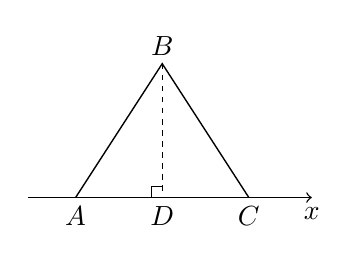
\begin{tikzpicture}[scale=1,line width=0.5pt]
\draw[->] (-0.4,0) -- (3.2,0) node[below] {$x$};
\draw (0.2,0) -- (1.3,1.7) -- (2.4,0);
\node at (0.2,-0.24) {$A$};
\node at (1.3,-0.24) {$D$};
\node at (2.4,-0.24) {$C$};
\node at (1.3,1.92) {$B$};
\draw[dash pattern=on 2pt off 2pt] (1.3,1.7) -- (1.3,0);
\draw (1.16,0) -- (1.16,0.14) -- (1.3,0.14);
\end{tikzpicture}
\end{center}
\step{$AB=AC=BC=\dfrac{2\sqrt3}3$，则 $x_2=x_1+AD=x_1+\dfrac{\sqrt3}3$，$x_3=x_1+\dfrac{2\sqrt3}3$，}
\step{存在 $x_1=-\dfrac{\sqrt3}3$，使得 $x_2=x_1+\dfrac{\sqrt3}3=0\in\Q$，且 $x_3=x_1+\dfrac{2\sqrt3}3=\dfrac{\sqrt3}3$ 为无理数，}
\step{即 $D(x_2)=1$，$D(x_3)=0$ 与图形一致，符合题意，}
\step{此时，$S_{\triangle ABC}=\dfrac12AC\cdot BD=\dfrac{\sqrt3}3$.}
\step{综上所述，存在这样的点 $A$、$B$、$C$，该正三角形的面积为 $\dfrac{\sqrt3}3$.}
\solend

\fi

\item 已知函数 $f(x)$ 满足：对 $\forall x\in R$，都有 $f(x+2025)\leqslant f(x)+2026$，
$f(x+2026)\geqslant f(x)+2027$，若 $f(1)=0$，则 $f(2)$ 的取值范围是\blankline[4.4em].

\ifanswer
\solbegin
\step{对 $\forall x\in R$，都有 $f(x+2025)\leqslant f(x)+2026$，$f(x+2026)\geqslant f(x)+2027$，}
\step{则 $f(x)+2027\leqslant f(x+2026)=f(x+1+2025)\leqslant f(x+1)+2026$，}
\step{即 $f(x)+1\leqslant f(x+1)$，所以 $f(2)\geqslant f(1)+1=1$；}
\step{$f(x)+2026\geqslant f(x+2025)=f(x+2024+1)\geqslant f(x+2024)+1$}
\step{$\geqslant\cdots\geqslant f(x+1)+2024$，所以 $f(x)+2\geqslant f(x+1)$，}
\step{所以 $f(2)\leqslant f(1)+2=2$；}
\step{即 $f(2)$ 的取值范围是 $[1,2]$.}
\solend

\fi

\end{enumerate}

\bigsec{二、选择题}

\begin{enumerate}
\setcounter{enumi}{12}

\item 若实数 $0<m<n<1$，而实数 $x>1$，则下列不等式正确的是\mbox{（\quad）}

\keepwithprev
A. $m^x<n^x$\qquad\qquad B. $x^m>x^n$\qquad\qquad C. $\log_xm>\log_xn$\qquad D. $\log_mx<\log_nx$

\ifanswer
\solbegin
\step{对于 $A$，函数 $f(t)=t^x$ 是以 $t$ 为变量，$x$ 为常量的幂函数，}
\step{由于 $x>1$，易得 $f(t)$ 在 $(0,+\infty)$ 上严格增，}
\step{$0<m<n<1$，$x>1$，可以得到 $m^x<n^x$，故 $A$ 正确；}
\step{对于 $B$，函数 $g(s)=x^s$，是以 $s$ 为变量，$x$ 为常量的指数函数，}
\step{由于 $x>1$，则 $g(s)$ 严格增，$0<m<n<1$，可以得到 $x^m<x^n$，故 $B$ 不正确；}
\step{对于 $C$，$\log_xm=\dfrac{\lg m}{\lg x}$，$\log_xn=\dfrac{\lg n}{\lg x}$，由于 $0<m<n<1$，则 $\lg m<\lg n<0$，}
\step{$x>1$，则 $\lg x>0$，则有 $\dfrac{\lg m}{\lg x}<\dfrac{\lg n}{\lg x}$，即 $\log_xm<\log_xn$，故 $C$ 不正确；}
\step{对于 $D$，由 $\log_mx-\log_nx=\dfrac{\lg x}{\lg m}-\dfrac{\lg x}{\lg n}=\dfrac{\lg x(\lg n-\lg m)}{\lg m\lg n}$，}
\step{因为实数 $0<m<n<1$，而实数 $x>1$，}
\step{所以 $\lg x>0$，$\lg m<\lg n<0$，则 $\dfrac{\lg x(\lg n-\lg m)}{\lg m\lg n}>0$，即 $\log_mx>\log_nx$，}
\step{故 $D$ 不正确.}
\step{故选 $A$.}
\solend

\fi

\item 已知 $x>1$，$y>1$，则 “$4^x>2^y$” 是 $\log_2x>\log_4(y-1)$ ”的\mbox{（\quad）}

\keepwithprev
A. 充分不必要条件\qquad\qquad B. 必要不充分条件

C. 充要条件\qquad\qquad D. 既不充分也不必要条件

\ifanswer
\solbegin
\step{因为 $x>1$，$y>1$，若 $4^x>2^y$，即 $2^{2x}>2^y$，所以 $2x>y>1$，}
\step{因为 $\dfrac y2-\sqrt{y-1}=\dfrac{(\sqrt{y-1})^2-2\sqrt{y-1}+1}2=\dfrac{(\sqrt{y-1}-1)^2}2\geqslant0$，}
\step{即 $\dfrac y2\geqslant\sqrt{y-1}>0$，所以 $\log_2\dfrac y2\geqslant\log_2\sqrt{y-1}=\dfrac12\log_2(y-1)=\log_4(y-1)$，}
\step{又 $x>\dfrac y2>\dfrac12$，所以 $\log_2x>\log_2\dfrac y2\geqslant\log_4(y-1)$，故充分性成立；}
\step{取 $x=2$，$y=4$，满足 $1=\log_2x>\log_4(y-1)=\log_43$，}
\step{但 $16=4^x=2^y=16$，即不满足 $4^x>2^y$，故必要性不成立.}% 链首链尾两个 16 系原卷笔误，应为 4^x=2^y=16，照录
\step{故选 $A$.}
\solend

\fi

\item 以下命题中，真命题的个数是\mbox{（\quad）}

①函数 $y=(x^2+1)^2+3$ 最小值为 3；②若 $2^a+\log_2a=4^b+2\log_4b$，则 $a<2b$；③不等式
$2^x-x-1>0$ 的解集为 $(1,+\infty)$.

\keepwithprev
A. $0$\qquad\qquad B. $1$\qquad\qquad C. $2$\qquad\qquad D. $3$

\ifanswer
\solbegin
\step{对于①，由于 $x^2+1\geqslant1$，则 $y=(x^2+1)^2+3\geqslant4$，}
\step{即函数 $y=(x^2+1)^2+3$ 最小值为 4，①错误；}
\step{对于②，由于 $b>0$，}
\step{则有 $2^a+\log_2a=4^b+2\log_4b=2^{2b}+\log_2b<2^{2b}+\log_22b$，}
\step{设 $f(x)=2^x+\log_2x$，易得 $f(x)$ 在 $(0,+\infty)$ 上为严格增函数，必有 $a<2b$，}
\step{②正确；}
\step{对于③，当 $x=-1$ 时，$2^x-x-1=2^x(x+1)>0$，即 $-1$ 在不等式的解集内，}
\step{③错误；}
\step{故选 $B$.}
\solend

\fi

\item 已知函数 $f(x)=ax^2+bx+c$（$a\neq0$ 且 $a<b$），若对任意的 $x\in R$，$f(x)\geqslant0$，且
$f(1)\geqslant\lambda(b-a)$，则实数 $\lambda$ 的取值范围为\mbox{（\quad）}

\keepwithprev
A. $(-\infty,2]$\qquad\qquad B. $[2\text{，}+\infty)$\qquad\qquad C. $(-\infty\text{，}3]$\qquad\qquad D. $[3\text{，}+\infty)$% 原卷 B/C/D 用全角逗号、A 用半角，照录

\ifanswer
\solbegin
\step{因为函数 $f(x)\geqslant0$ 恒成立，所以 $a>0$，且 $\Delta=b^2-4ac\leqslant0$，即 $c\geqslant\dfrac{b^2}{4a}$，}
\step{所以 $a+b+c\geqslant a+b+\dfrac{b^2}{4a}$，又 $a<b$，所以 $b-a>0$，}
\step{又 $f(1)\geqslant\lambda(b-a)$ 恒成立，所以 $a+b+c\geqslant\lambda(b-a)$ 恒成立，}
\step{即 $\lambda\leqslant\left(\dfrac{a+b+c}{b-a}\right)_{\min}=\dfrac{a+b+\dfrac{b^2}{4a}}{b-a}$，}
\step{令 $t=\dfrac ba$（$t>1$），则 $\dfrac{a+b+\dfrac{b^2}{4a}}{b-a}=\dfrac{1+t+\dfrac{t^2}4}{t-1}$，}
\step{令 $\mu=t-1$（$\mu>0$），则 $t=\mu+1$，}
\step{故上式 $=\dfrac{1+\mu+1+\dfrac{(\mu+1)^2}4}{\mu}=\dfrac14\left(\mu+\dfrac9\mu+6\right)$，}
\step{对 $\mu>0$，有 $\mu+\dfrac9\mu\geqslant2\sqrt{\mu\times\dfrac9\mu}=6$，当且仅当 $\mu=\dfrac9\mu$，即 $\mu=3$ 时取等号，}
\step{所以 $\dfrac14\left(\mu+\dfrac9\mu+6\right)\geqslant\dfrac14(6+6)=3$，故 $\lambda\leqslant3$，}
\step{即实数 $\lambda$ 的取值范围为 $(-\infty,3]$. 故选 $C$.}
\solend

\fi

\end{enumerate}

\bigsec{三、解答题}

\begin{enumerate}
\setcounter{enumi}{16}

\item 已知函数 $f(x)=\log_\frac23(ax^2-6x+18)$.

（1）若 $f(x)$ 的定义域为 $R$，求实数 $a$ 的取值范围.

（2）若 $f(x)$ 的值域为 $R$，求实数 $a$ 的取值范围.

\ansspace*[10]

\ifanswer
\solbegin
\stepm{（1）}{由 $f(x)=\log_\frac23(ax^2-6x+18)$ 的定义域为 $R$，得 $ax^2-6x+18>0$ 恒成立，}
\step{$a=0$ 时，$f(x)=\log_\frac23(18-6x)$ 的定义域为 $(-\infty,3)$，不符合题意.}
\step{$a\neq0$ 时，$\begin{cases}a>0\\ \Delta=36-4\times18a<0\end{cases}$，解得 $a>\dfrac12$.}
\step{综上，$a$ 的取值范围是 $\left(\dfrac12,+\infty\right)$.}
\stepm{（2）}{$a=0$ 时，$f(x)=\log_\frac23(18-6x)$ 的值域为 $R$，符合题意.}
\step{$a\neq0$ 时，$\begin{cases}a>0\\ \Delta=36-4\times18a\geqslant0\end{cases}$，解得 $0<a\leqslant\dfrac12$.}
\step{综上，$a$ 的取值范围是 $\left[0,\dfrac12\right]$.}
\solend

\fi

\item 已知 $f(x)=\log_ax+\log_a(6-x)$，$a>0$ 且 $a\neq1$，且 $f(3)=2$.

（1）求 $a$ 的值及 $f(x)$ 的单调区间.

（2）若对于 $\forall x_1\in(0,6)$，$\exists x_2\in[1,9]$，使得 $f(x_1)\leqslant t+\log_3x_2$ 成立，求实数 $t$ 的取值范
围.

\ansspace*[12]

\ifanswer
\solbegin
\stepm{（1）}{已知 $f(x)=\log_ax+\log_a(6-x)$，且 $f(3)=2$.}
\step{得 $\log_a3+\log_a(6-3)=2$，即 $2\log_a3=2$，}
\step{因此 $\log_a3=1$，因此 $a=3$，因此 $f(x)=\log_3x+\log_3(6-x)$，}
\step{因为 $\begin{cases}x>0\\ 6-x>0\end{cases}$，因此 $0<x<6$，故 $f(x)$ 的定义域为 $(0,6)$；}
\step{$f(x)=\log_3(6x-x^2)$，}
\step{因为函数 $y=6x-x^2$ 在 $(0,3)$ 上严格增，在 $(3,6)$ 上严格减，}
\step{又函数 $y=\log_3x$ 为严格增函数，}
\step{由复合函数的单调性得函数 $f(x)$ 在 $(0,3)$ 上严格增，在 $(3,6)$ 上严格减；}
\stepm{（2）}{令 $g(x)=t+\log_3x$，}
\step{因为 $\forall x_1\in(0,6)$，$\exists x_2\in[1,9]$，使得 $f(x_1)\leqslant t+\log_3x_2$，}
\step{即 $f(x_{1})_{\max}\leqslant g(x_{2})_{\max}$，}
\step{其中由（1）得 $f(x_{1})_{\max}=f(3)=2$.}
\step{又 $g(x)=t+\log_3x$ 在 $[1,9]$ 上严格增，因此 $g(x)_{\max}=g(9)=t+2$，}
\step{因此 $2\leqslant t+2$，因此实数 $t$ 的取值范围为 $[0,+\infty)$.}
\solend

\fi

\item 某心理学研究小组在对学生上课注意力集中情况的调查研究中，发现其注意力指数 $p$ 与
听课时间 $t$ 之间的关系满足如图所示的曲线. 当 $t\in(0,14]$ 时，曲线是二次函数图象的一部
分，当 $t\in[14,40]$ 时，曲线是函数 $y=\log_a(t-5)+83$（$a>0$ 且 $a\neq1$）图象的一部分. 根据
专家研究，当注意力指数 $p$ 大于等于 80 时听课效果最佳.

（1）试求 $p=f(t)$ 的函数关系式；

（2）当一位学生在坚持听课 32 分钟时，注意力指数 $p$ 大约为多少？

（3）一道数学难题，讲解需要 20 分钟，问老师能否经过合理安排在学生听
课效果最佳时讲完？请说明理由.

\begin{center}
% 原图第 9 页题干 p-t 曲线图按原图形状用 TikZ 重排（三版都出）。
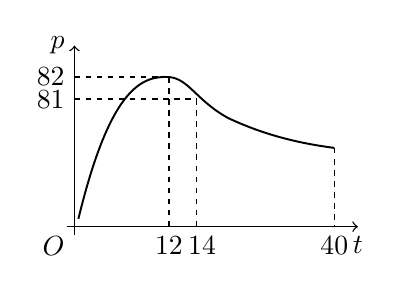
\begin{tikzpicture}[scale=1,line width=0.5pt]
\draw[->] (-0.1,0) -- (3.6,0) node[below] {$t$};
\draw[->] (0,-0.1) -- (0,2.3) node[left] {$p$};
\node[below left] at (0,0) {$O$};
\draw[line width=0.7pt] (0.05,0.1) .. controls (0.45,1.75) and (0.85,1.92) .. (1.2,1.9)
  .. controls (1.45,1.88) and (1.55,1.6) .. (1.95,1.38)
  .. controls (2.5,1.12) and (3.0,1.04) .. (3.3,1.0);
\draw[dash pattern=on 2pt off 2pt] (0,1.9) -- (1.2,1.9);
\draw[dash pattern=on 2pt off 2pt] (0,1.62) -- (1.55,1.62);
\draw[dash pattern=on 2pt off 2pt] (1.2,1.9) -- (1.2,0);
\draw[dash pattern=on 2pt off 2pt] (1.55,1.62) -- (1.55,0);
\draw[dash pattern=on 2pt off 2pt] (3.3,1.0) -- (3.3,0);
\node[left] at (0,1.9) {$82$};
\node[left] at (0,1.62) {$81$};
\node[below] at (1.2,0) {$12$};
\node[below] at (1.62,0) {$14$};
\node[below] at (3.3,0) {$40$};
\end{tikzpicture}
\end{center}

\ansspace*[12]

\ifanswer
\solbegin
\stepm{（1）}{由题意得当 $t\in(0,14]$ 时，设 $f(t)=c(t-12)^2+82$（$c<0$），}
\step{又 $f(14)=81$，所以 $c(14-12)^2+82=81$，解得 $c=-\dfrac14$；}
\step{所以 $f(t)=-\dfrac14(t-12)^2+82$,$t\in(0,14]$；}
\step{又当 $t\in[14,40]$ 时，函数 $y=\log_a(t-5)+83$（$a>0$ 且 $a\neq1$），}
\step{又当 $x=14$ 时，$y=81$，所以 $81=\log_a(14-5)+83$，解得 $a=\dfrac13$；}
\step{所以 $f(t)=\log_\frac13(t-5)+83$,$t\in[14,40]$，}
\step{所以 $p=\begin{cases}-\dfrac14(t-12)^2+82, & t\in(0,14]\\ \log_\frac13(t-5)+83, & t\in(14,40]\end{cases}$；}
\stepm{（2）}{当 $t=32$ 时，$p=\log_\frac13(32-5)+83=80$，}
\step{所以当一位学生在坚持听课 32 分钟时，注意力指数 $p$ 大约为 80；}
\stepm{（3）}{当 $t\in(0,14]$ 时，$-\dfrac14(t-12)^2+82\geqslant80$，解得 $t\in[12-2\sqrt2,14]$，}
\step{当 $t\in[14,40]$ 时，$\log_\frac13(t-5)+83\geqslant80$，解得 $5<t\leqslant32$，则 $t\in[14,32]$，}
\step{因此当 $t\in[12-2\sqrt2,32]$ 时学生听课效果最佳，}
\step{此时 $\Delta t=32-(12-2\sqrt2)=20+2\sqrt2>20$，}
\step{所以老师能经过合理安排时间在学生听课效果最佳时段讲完.}
\solend

\fi

\item 已知 $a\in R$，函数 $f(x+1)=\log_2\left(\dfrac{ax+1+a}{x+1}\right)$.

（1）若 $a=2$，求函数 $f(x)$ 的表达式及定义域；

（2）若关于 $x$ 的方程 $f\left(\dfrac x2\right)-\log_2[(a-2)x+3a-5]=0$ 的解集中恰好只有一个元素，求实
数 $a$ 的取值范围.

\ansspace*[14]

\ifanswer
\solbegin
\stepm{（1）}{$f(x+1)=\log_2\left(\dfrac{ax+1+a}{x+1}\right)$，}
\step{令 $x+1=t$，则 $f(t)=\log_2\left(\dfrac1t+a\right)$，即 $f(x)=\log_2\left(\dfrac1x+a\right)$，}
\step{因为 $a=2$，所以 $f(x)=\log_2\left(2+\dfrac1x\right)$，}
\step{由 $2+\dfrac1x>0$ 得定义域为 $\left(-\infty,-\dfrac12\right)\cup(0,+\infty)$；}
\stepm{（2）}{由（1）得 $f(x)=\log_2\left(\dfrac1x+a\right)$，}
\step{方程 $f\left(\dfrac x2\right)-\log_2[(a-2)x+3a-5]=0$，}
\step{即 $\log_2\left(\dfrac2x+a\right)-\log_2[(a-2)x+3a-5]=0$，}
\step{可转化为 $(a-2)x^2+(2a-5)x-2=0$，且 $\dfrac2x+a>0$.}
\step{①当 $a-2=0$，即 $a=2$ 时，$x=-2$，符合题意；}
\step{②当 $a-2\neq0$，即 $a\neq2$ 时，$x_1=-2$,$x_2=\dfrac1{a-2}$，}
\step{（$i$）当 $-2=\dfrac1{a-2}$ 时，即 $a=\dfrac32$ 时，符合题意；}
\step{（$ii$）当 $-2\neq\dfrac1{a-2}$ 时，即 $a\neq\dfrac32$ 且 $a\neq2$ 时，}
\step{要满足题意，则有 $\begin{cases}-1+a>0\\ 3a-4\leqslant0\end{cases}\Rightarrow1<a\leqslant\dfrac43$ 或 $\begin{cases}-1+a\leqslant0\\ 3a-4>0\end{cases}$，无解；}
\step{综上，$a$ 的取值范围 $\left(1,\dfrac43\right]\cup\left\{2,\dfrac32\right\}$.}
\solend

\fi

\item 已知函数 $y=f(x)$ 是定义在 $[0,+\infty)$ 上的函数，并且 $f(x)\geqslant0$，对于定义域内的任意自
变量的值 $x$、$y$，满足 $f(y)f(x^2f(y)+xf(y))=f(x^2+y+x)$，$f(a)=0$，其中
$a>0$.

（1）当 $f(0)\neq0$ 时，求 $f(0)$；

（2）已知当 $0\leqslant x<a$ 时，有 $f(x)\neq0$.

（$i$）求 $f(a+3)$；

（$ii$）求函数 $y=f(x)$ 的解析式（用 $a$ 表示）.

\ansspace*[16]

\ifanswer
\solbegin
\stepm{（1）}{因为 $f(x)\geqslant0$，且对于定义域内的任意自变量的值 $x$、$y$，}
\step{满足 $f(y)f(x^2f(y)+xf(y))=f(x^2+y+x)$，}
\step{令 $x=y=0$，则 $f^2(0)=f(0)$，因为 $f(0)\neq0$，所以 $f(0)=1$，}
\stepm{（2）}{（$i$）由 $f(y)f(x^2f(y)+xf(y))=f(x^2+y+x)$，}
\step{得 $f(y)f[(x^2+x)f(y)]=f[(x^2+x)+y]$，}
\step{令 $t=x^2+x$，因为 $x\geqslant0$，所以 $t=x^2+x\in[0,+\infty)$，}
\step{所以有 $f(y)f(tf(y))=f(t+y)$，因为 $f(a)=0$，}
\step{令 $y=a$，$t=3$，得 $f(a+3)=f(a)f(3f(a))=0\times f(3f(a))=0$；}
\step{（$ii$）当 $x\geqslant a$ 时，令 $y=a$，$t=x-a$，}
\step{$f(x)=f(x-a+a)=f(a)f[(x-a)f(a)]=0$.}
\step{当 $0\leqslant x<a$ 时，则有 $0<a-x\leqslant a$，令 $y=x$，$t=a-x$，}
\step{则 $f(a)=f(a-x+x)=f(x)f[(a-x)f(x)]=0$.}
\step{因为 $f(x)\neq0$，所以有 $f((a-x)f(x))=0$，则 $(a-x)f(x)\geqslant a$，}
\step{又因为 $a-x>0$，即 $f(x)\geqslant\dfrac a{a-x}$.}
\step{令 $t=\dfrac a{f(x)}>0$,$y=x>0$，}
\step{则 $f\left(\dfrac a{f(x)}+x\right)=f(x)\cdot f\left(\dfrac a{f(x)}\cdot f(x)\right)=f(x)\cdot f(a)=0$，}
\step{所以有 $\dfrac a{f(x)}+x\geqslant a$，即 $\dfrac a{f(x)}\geqslant a-x$，得 $f(x)\leqslant\dfrac a{a-x}$，}
\step{所以当 $0\leqslant x<a$ 时，$f(x)=\dfrac a{a-x}$.}
\step{综上，$f(x)=\begin{cases}\dfrac a{a-x}, & 0\leqslant x<a\\ 0, & x\geqslant a\end{cases}$.}
\solend

\fi

\end{enumerate}

\end{document}
"
% 紧凑版：xelatex "\def\iscompact{1}% 高一105_交附闵行_周末作业10.30.tex
%   —— 高一上数学“2026-2027 年交附闵行高一上周末作业 10.30”（试卷版/答案版）
% 试卷版：xelatex 高一105_交附闵行_周末作业10.30.tex
% 答案版：xelatex "\def\isanswer{1}% 高一105_交附闵行_周末作业10.30.tex
%   —— 高一上数学“2026-2027 年交附闵行高一上周末作业 10.30”（试卷版/答案版）
% 试卷版：xelatex 高一105_交附闵行_周末作业10.30.tex
% 答案版：xelatex "\def\isanswer{1}% 高一105_交附闵行_周末作业10.30.tex
%   —— 高一上数学“2026-2027 年交附闵行高一上周末作业 10.30”（试卷版/答案版）
% 试卷版：xelatex 高一105_交附闵行_周末作业10.30.tex
% 答案版：xelatex "\def\isanswer{1}\input{高一105_交附闵行_周末作业10.30.tex}"
% 紧凑版：xelatex "\def\iscompact{1}\input{高一105_交附闵行_周末作业10.30.tex}"
%
% 原始材料：微信公众号“魔都数学加油站”文章，作者破晓，2026-11-02 17:41 发布；
% 连载“27学年高一105”，原文标题“27学年高一105——2026-2027年上海市交附闵行高一上周末作业10.30”；
% 原文链接：https://mp.weixin.qq.com/s/XUfNEvGHjD0CB5jdoleBWw。
% 正文为 13 张 PNG 页（第 4、9、13 页 2560×3620，其余 4762×6735），题目下印有【解析】，为讲评版。
% 题目、解析均据原图转录；卷面水印及公众号页脚未录入。
%
% 卷首标题：原卷印作“2026-2027 年交附闵行高一上周末作业 10.30”（公众号标题中的“上海市”
% 卷面标题行没有，本稿照卷面），年份区间按全稿惯例排 en dash；原卷未印副标题，本稿按题目
% 内容标为“函数、不等式”（主体为指数与对数，第 3 题集合、第 16 题基本不等式）。
%
% 与原卷的排版差异：
%   ① 原文从第 3 题起，填空题编号为 3—12、选择题为 13—16、解答题为 17—21，本稿保留原题号；
%   ② 原卷每题下直接印【解析】，本稿按全稿惯例将解析置于答案版；选择题括号内未印答案，另由
%      解析末句“故选 X”给出；
%   ③ 原卷未印副标题，本稿按“知识模块”口径补出；
%   ④ 原卷填空横线按全稿惯例排为 \blankline[4.4em]；解答题按惯例加 \ansspace；选择题括号排
%      \mbox{（\quad）}、选项段前按惯例加 \keepwithprev；
%   ⑤ $f(x_1)_{max}$、$g(x)_max$、$\left(\frac{a+b+c}{b-a}\right)_{min}$ 等下标原卷排斜体，
%      按 高一96 成例改正体 $\max$、$\min$；
%   ⑥ 原卷数集排斜体 $R$／$Q$，按全稿惯例改 $\R$／$\Q$；
%   ⑦ 第 11 题解析的两幅三角形示意图与第 19 题题干的 $p$-$t$ 曲线图均按原图形状用 TikZ 重排
%      （第 19 题图属题干、三版都出；第 11 题图属解析、仅答案版显示）。
%
% 原卷存疑／笔误（均照录加注）：
%   第 14 题解析“但 $16=4^x=2^y=16$”（链首、链尾的两个 $16$ 系原卷笔误，按上下文应为
%   $4^x=2^y=16$）；
%   第 16 题选项的区间分隔逗号 A 项排半角、B／C／D 三项排全角（原卷自身不一致）；
%   第 21 题 (2) 的小问号排“（$i$）求…”（右括号紧贴“求”字），照录。
%
% 行数核对：逐题数 \step/\stepm 条数，合计 159 条（Q3：2；Q4：1；Q5：4；Q6：6；Q7：3；
% Q8：7；Q9：5；Q10：3；Q11：15；Q12：7；Q13：12；Q14：7；Q15：9；Q16：10；Q17：7；
% Q18：14；Q19：14；Q20：14；Q21：19），与原卷印刷行逐题相等。
%
\documentclass[a4paper,11pt]{article}
\usepackage{common}

\begin{document}

\examtitlest[3]{2026--2027 年交附闵行高一上周末作业 10.30}{函数、不等式}

\bigsec{一、填空题}

\begin{enumerate}
\setcounter{enumi}{2}

\item 已知集合 $M=\{1,m\}$，$N=\{n,\log_2n\}$，若 $M=N$，则 $(m-n)^{2027}=$\blankline[4.4em].

\ifanswer
\solbegin
\step{由题意得 $\begin{cases}n=1\\ \log_2n=m\end{cases}$ 或 $\begin{cases}n=m\\ \log_2n=1\end{cases}$，解得 $\begin{cases}n=1\\ m=0\end{cases}$ 或 $\begin{cases}n=2\\ m=2\end{cases}$，}
\step{所以 $(m-n)^{2027}=-1$ 或 $0$.}
\solend

\fi

\item 已知 $\log_{2x^2-1}(3x^2+2x-1)=1$，则 $x=$\blankline[4.4em].

\ifanswer
\solbegin
\step{因为 $\log_{2x^2-1}(3x^2+2x-1)=1$，所以 $\begin{cases}2x^2-1>0\\ 2x^2-1\neq1\\ 3x^2+2x-1>0\\ 2x^2-1=3x^2+2x-1\end{cases}$，解得 $x=-2$.}
\solend

\fi

\item 已知 $m>1$，$n>1$，$\lg m=\log_n100$，则 $mn$ 的最小值为\blankline[4.4em].

\ifanswer
\solbegin
\step{由 $m>1$，$n>1$，得 $\lg m>0$，$\lg n>0$，}
\step{因为 $\lg m=\log_n100=\dfrac{\lg100}{\lg n}=\dfrac2{\lg n}$，所以 $\lg m\cdot\lg n=2$，}
\step{所以 $\lg(mn)=\lg m+\lg n\geqslant2\sqrt{\lg m\cdot\lg n}=2\sqrt2$，}
\step{当且仅当 $m=n=10^{\sqrt2}$ 时取等号，则 $mn\geqslant10^{2\sqrt2}$，即 $mn$ 的最小值为 $10^{2\sqrt2}$.}
\solend

\fi

\item 设 $m$、$n$ 分别是方程 $\log_{2013}x+x-9=0$ 和 $2013^x+x-9=0$ 的根，则 $m+n=$\blankline[4.4em].

\ifanswer
\solbegin
\step{由 $\log_{2013}x+x-9=0$，得 $\log_{2013}x=-x+9$，}
\step{因为 $m$ 是方程 $\log_{2013}x+x-9=0$ 的根，}
\step{所以 $m$ 为函数 $y=\log_{2013}x$ 与 $y=-x+9$ 图象交点的横坐标，}
\step{同理 $n$ 是函数 $y=2013^x$ 与 $y=-x+9$ 图象交点的横坐标，}
\step{因为 $y=\log_{2013}x$ 与 $y=2013^x$ 互为反函数，其图象关于直线 $y=x$ 对称，}
\step{联立 $\begin{cases}y=-x+9\\ y=x\end{cases}$，解得 $x=\dfrac92$，所以 $m+n=\dfrac92\times2=9$.}
\solend

\fi

\item 已知函数 $f(x)=\dfrac1{\log_2(x^2+4)}$，则 $f(-2)=$\blankline[2em]，$f(x)$ 的值域为\blankline[4.4em].

\ifanswer
\solbegin
\step{$f(-2)=\dfrac1{\log_28}=\dfrac13$.}
\step{因为 $x^2+4\geqslant4$，所以 $\log_2(x^2+4)\geqslant\log_24=2$，所以 $0<\dfrac1{\log_2(x^2+4)}\leqslant\dfrac12$，}
\step{故 $f(x)$ 的值域为 $\left(0,\dfrac12\right]$.}
\solend

\fi

\item 已知 $\alpha$、$\beta$ 是方程 $9^x-2m\cdot3^x+m^2-1=0$ 的两个根，若 $\alpha+\beta=1$，则 $\alpha\beta=$\blankline[4.4em].

\ifanswer
\solbegin
\step{由题意得方程 $9^x-2m\cdot3^x+m^2-1=0$ 有两个根，}
\step{则方程 $t^2-2mt+m^2-1=0$ 有二正根，}
\step{则 $\begin{cases}\Delta=4m^2-4(m^2-1)\geqslant0\\ 2m>0\\ m^2-1>0\end{cases}$，解得 $m>1$，}
\step{又 $\alpha$、$\beta$ 是方程 $9^x-2m\cdot3^x+m^2-1=0$ 的两个根，}
\step{则 $3^\alpha\times3^\beta=m^2-1$，又 $\alpha+\beta=1$，则 $m^2-1=3^{\alpha+\beta}=3$，}
\step{解得 $m=2$ 或 $m=-2$（舍），则 $3^\alpha+3^\beta=2m=4$，又 $\alpha=1-\beta$，}
\step{则 $3^{1-\beta}+3^\beta=4$，解得 $\beta=0$ 或 $\beta=1$，则 $\begin{cases}\alpha=1\\ \beta=0\end{cases}$ 或 $\begin{cases}\alpha=0\\ \beta=1\end{cases}$，则 $\alpha\beta=0$.}
\solend

\fi

\item 已知 $a>b>0$，$\ln a=2\ln b$，且 $a\lg b=b\lg a$，则 $a+b=$\blankline[4.4em].

\ifanswer
\solbegin
\step{因为 $a>b>0$，$\ln a=2\ln b=\ln b^2$，所以 $a=b^2$，}
\step{由 $a\lg b=b\lg a$ 得 $b^2\lg b=b\lg b^2$，即 $b\lg b=2\lg b$，所以 $b=1$ 或 $b=2$，}
\step{当 $b=2$，$a=4$，满足题意，}
\step{当 $b=1$ 时，$a=1$ 与 $a>b>0$ 矛盾，所以 $b=1$ 舍去，}
\step{所以 $a+b=6$.}
\solend

\fi

\item 函数 $f(x)=\begin{cases}2^x, & x\leqslant t\\ \log_\frac12x, & x>t\end{cases}$ 的值域为 $M$，且 $8\notin M$，则实数 $t$ 的取值集合为\blankline[4.4em].

\ifanswer
\solbegin
\step{当 $x\leqslant t$ 时，函数 $f(x)=2^x$ 在 $(-\infty,t]$ 严格增，}
\step{当 $x>t$ 时，$f(x)=\log_\frac12x$ 在 $(t,+\infty)$ 严格减，}
\step{若 $8\notin M$，则满足条件 $\begin{cases}2^t<8\\ \log_\frac12t\leqslant8\end{cases}\Rightarrow\dfrac1{256}\leqslant t<3$，故实数 $t$ 的取值集合为 $\left[\dfrac1{256},3\right)$.}
\solend

\fi

\item 德国数学家狄利克雷在数学领域成就显著，以其命名函数 $D(x)=\begin{cases}1, & x\text{为有理数}\\ 0, & x\text{为无理数}\end{cases}$，该函
数被称为狄利克雷函数。那么是否存在三个点 $A(x_1,D(x_1))$、$B(x_2,D(x_2))$、$C(x_3,D(x_3))$，
使得 $\triangle ABC$ 为等边三角形，若不存在请在横线上填写“不存在”，如果存在则在横线上填写
该正三角形的面积\blankline[4.4em].

\ifanswer
\solbegin
\step{因为 $D(x)=\begin{cases}1, & x\text{为有理数}\\ 0, & x\text{为无理数}\end{cases}$，所以 $D(x)=0$ 或 1，}
\step{设存在三个点 $A(x_1,D(x_1))$、$B(x_2,D(x_2))$、$C(x_3,D(x_3))$，}
\step{使得 $\triangle ABC$ 为等边三角形，则 $D(x_1)$、$D(x_2)$、$D(x_3)$ 不同时为 0 或 1，}
\step{不妨设 $x_1<x_2<x_3$，分析得 $\triangle ABC$ 的位置有两种情况，}
\step{第一种情况：当 $x_1$ 为有理数时，即 $D(x_1)=1$，如图，过点 $B$ 作 $BD\perp AC$，}
\begin{center}
% 原图第 4 页解析示意图按原图形状用 TikZ 重排（第一种情况：$B$ 在 $x$ 轴上、$AC$ 在上方）。
\begin{tikzpicture}[scale=1,line width=0.5pt]
\draw (0,1.2) -- (2.6,1.2);
\node at (0.25,1.4) {$A$};
\node at (1.3,1.4) {$D$};
\node at (2.35,1.4) {$C$};
\draw[dash pattern=on 2pt off 2pt] (1.3,1.2) -- (1.3,0);
\draw (1.16,1.2) -- (1.16,1.06) -- (1.3,1.06);
\draw[->] (-0.5,0) -- (3.1,0) node[below] {$x$};
\node at (1.3,-0.24) {$B$};
\end{tikzpicture}
\end{center}
\step{垂足为 $D$，得 $BD=1$，$AD=\dfrac{\sqrt3}3$，$AB=AC=BC=\dfrac{2\sqrt3}3$，}
\step{则 $x_2=x_1+AD=x_1+\dfrac{\sqrt3}3$ 为无理数，$x_3=x_1+\dfrac{2\sqrt3}3$ 为无理数，}
\step{即 $D(x_2)=0$，$D(x_3)=0$ 与图形不一致，舍去；}
\step{第二种情况：当 $x_1$ 为无理数时，即 $D(x_1)=0$，如图，}
\step{过点 $B$ 作 $BD\perp AC$，垂足为 $D$，得 $BD=1$，$AD=\dfrac{\sqrt3}3$，}
\begin{center}
% 原图第 4 页解析示意图按原图形状用 TikZ 重排（第二种情况：$B$ 在上方、$AC$ 在 $x$ 轴上）。
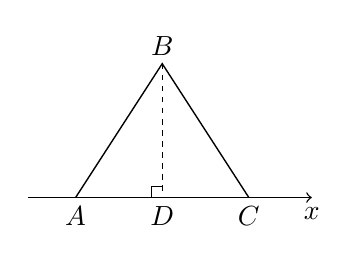
\begin{tikzpicture}[scale=1,line width=0.5pt]
\draw[->] (-0.4,0) -- (3.2,0) node[below] {$x$};
\draw (0.2,0) -- (1.3,1.7) -- (2.4,0);
\node at (0.2,-0.24) {$A$};
\node at (1.3,-0.24) {$D$};
\node at (2.4,-0.24) {$C$};
\node at (1.3,1.92) {$B$};
\draw[dash pattern=on 2pt off 2pt] (1.3,1.7) -- (1.3,0);
\draw (1.16,0) -- (1.16,0.14) -- (1.3,0.14);
\end{tikzpicture}
\end{center}
\step{$AB=AC=BC=\dfrac{2\sqrt3}3$，则 $x_2=x_1+AD=x_1+\dfrac{\sqrt3}3$，$x_3=x_1+\dfrac{2\sqrt3}3$，}
\step{存在 $x_1=-\dfrac{\sqrt3}3$，使得 $x_2=x_1+\dfrac{\sqrt3}3=0\in\Q$，且 $x_3=x_1+\dfrac{2\sqrt3}3=\dfrac{\sqrt3}3$ 为无理数，}
\step{即 $D(x_2)=1$，$D(x_3)=0$ 与图形一致，符合题意，}
\step{此时，$S_{\triangle ABC}=\dfrac12AC\cdot BD=\dfrac{\sqrt3}3$.}
\step{综上所述，存在这样的点 $A$、$B$、$C$，该正三角形的面积为 $\dfrac{\sqrt3}3$.}
\solend

\fi

\item 已知函数 $f(x)$ 满足：对 $\forall x\in R$，都有 $f(x+2025)\leqslant f(x)+2026$，
$f(x+2026)\geqslant f(x)+2027$，若 $f(1)=0$，则 $f(2)$ 的取值范围是\blankline[4.4em].

\ifanswer
\solbegin
\step{对 $\forall x\in R$，都有 $f(x+2025)\leqslant f(x)+2026$，$f(x+2026)\geqslant f(x)+2027$，}
\step{则 $f(x)+2027\leqslant f(x+2026)=f(x+1+2025)\leqslant f(x+1)+2026$，}
\step{即 $f(x)+1\leqslant f(x+1)$，所以 $f(2)\geqslant f(1)+1=1$；}
\step{$f(x)+2026\geqslant f(x+2025)=f(x+2024+1)\geqslant f(x+2024)+1$}
\step{$\geqslant\cdots\geqslant f(x+1)+2024$，所以 $f(x)+2\geqslant f(x+1)$，}
\step{所以 $f(2)\leqslant f(1)+2=2$；}
\step{即 $f(2)$ 的取值范围是 $[1,2]$.}
\solend

\fi

\end{enumerate}

\bigsec{二、选择题}

\begin{enumerate}
\setcounter{enumi}{12}

\item 若实数 $0<m<n<1$，而实数 $x>1$，则下列不等式正确的是\mbox{（\quad）}

\keepwithprev
A. $m^x<n^x$\qquad\qquad B. $x^m>x^n$\qquad\qquad C. $\log_xm>\log_xn$\qquad D. $\log_mx<\log_nx$

\ifanswer
\solbegin
\step{对于 $A$，函数 $f(t)=t^x$ 是以 $t$ 为变量，$x$ 为常量的幂函数，}
\step{由于 $x>1$，易得 $f(t)$ 在 $(0,+\infty)$ 上严格增，}
\step{$0<m<n<1$，$x>1$，可以得到 $m^x<n^x$，故 $A$ 正确；}
\step{对于 $B$，函数 $g(s)=x^s$，是以 $s$ 为变量，$x$ 为常量的指数函数，}
\step{由于 $x>1$，则 $g(s)$ 严格增，$0<m<n<1$，可以得到 $x^m<x^n$，故 $B$ 不正确；}
\step{对于 $C$，$\log_xm=\dfrac{\lg m}{\lg x}$，$\log_xn=\dfrac{\lg n}{\lg x}$，由于 $0<m<n<1$，则 $\lg m<\lg n<0$，}
\step{$x>1$，则 $\lg x>0$，则有 $\dfrac{\lg m}{\lg x}<\dfrac{\lg n}{\lg x}$，即 $\log_xm<\log_xn$，故 $C$ 不正确；}
\step{对于 $D$，由 $\log_mx-\log_nx=\dfrac{\lg x}{\lg m}-\dfrac{\lg x}{\lg n}=\dfrac{\lg x(\lg n-\lg m)}{\lg m\lg n}$，}
\step{因为实数 $0<m<n<1$，而实数 $x>1$，}
\step{所以 $\lg x>0$，$\lg m<\lg n<0$，则 $\dfrac{\lg x(\lg n-\lg m)}{\lg m\lg n}>0$，即 $\log_mx>\log_nx$，}
\step{故 $D$ 不正确.}
\step{故选 $A$.}
\solend

\fi

\item 已知 $x>1$，$y>1$，则 “$4^x>2^y$” 是 $\log_2x>\log_4(y-1)$ ”的\mbox{（\quad）}

\keepwithprev
A. 充分不必要条件\qquad\qquad B. 必要不充分条件

C. 充要条件\qquad\qquad D. 既不充分也不必要条件

\ifanswer
\solbegin
\step{因为 $x>1$，$y>1$，若 $4^x>2^y$，即 $2^{2x}>2^y$，所以 $2x>y>1$，}
\step{因为 $\dfrac y2-\sqrt{y-1}=\dfrac{(\sqrt{y-1})^2-2\sqrt{y-1}+1}2=\dfrac{(\sqrt{y-1}-1)^2}2\geqslant0$，}
\step{即 $\dfrac y2\geqslant\sqrt{y-1}>0$，所以 $\log_2\dfrac y2\geqslant\log_2\sqrt{y-1}=\dfrac12\log_2(y-1)=\log_4(y-1)$，}
\step{又 $x>\dfrac y2>\dfrac12$，所以 $\log_2x>\log_2\dfrac y2\geqslant\log_4(y-1)$，故充分性成立；}
\step{取 $x=2$，$y=4$，满足 $1=\log_2x>\log_4(y-1)=\log_43$，}
\step{但 $16=4^x=2^y=16$，即不满足 $4^x>2^y$，故必要性不成立.}% 链首链尾两个 16 系原卷笔误，应为 4^x=2^y=16，照录
\step{故选 $A$.}
\solend

\fi

\item 以下命题中，真命题的个数是\mbox{（\quad）}

①函数 $y=(x^2+1)^2+3$ 最小值为 3；②若 $2^a+\log_2a=4^b+2\log_4b$，则 $a<2b$；③不等式
$2^x-x-1>0$ 的解集为 $(1,+\infty)$.

\keepwithprev
A. $0$\qquad\qquad B. $1$\qquad\qquad C. $2$\qquad\qquad D. $3$

\ifanswer
\solbegin
\step{对于①，由于 $x^2+1\geqslant1$，则 $y=(x^2+1)^2+3\geqslant4$，}
\step{即函数 $y=(x^2+1)^2+3$ 最小值为 4，①错误；}
\step{对于②，由于 $b>0$，}
\step{则有 $2^a+\log_2a=4^b+2\log_4b=2^{2b}+\log_2b<2^{2b}+\log_22b$，}
\step{设 $f(x)=2^x+\log_2x$，易得 $f(x)$ 在 $(0,+\infty)$ 上为严格增函数，必有 $a<2b$，}
\step{②正确；}
\step{对于③，当 $x=-1$ 时，$2^x-x-1=2^x(x+1)>0$，即 $-1$ 在不等式的解集内，}
\step{③错误；}
\step{故选 $B$.}
\solend

\fi

\item 已知函数 $f(x)=ax^2+bx+c$（$a\neq0$ 且 $a<b$），若对任意的 $x\in R$，$f(x)\geqslant0$，且
$f(1)\geqslant\lambda(b-a)$，则实数 $\lambda$ 的取值范围为\mbox{（\quad）}

\keepwithprev
A. $(-\infty,2]$\qquad\qquad B. $[2\text{，}+\infty)$\qquad\qquad C. $(-\infty\text{，}3]$\qquad\qquad D. $[3\text{，}+\infty)$% 原卷 B/C/D 用全角逗号、A 用半角，照录

\ifanswer
\solbegin
\step{因为函数 $f(x)\geqslant0$ 恒成立，所以 $a>0$，且 $\Delta=b^2-4ac\leqslant0$，即 $c\geqslant\dfrac{b^2}{4a}$，}
\step{所以 $a+b+c\geqslant a+b+\dfrac{b^2}{4a}$，又 $a<b$，所以 $b-a>0$，}
\step{又 $f(1)\geqslant\lambda(b-a)$ 恒成立，所以 $a+b+c\geqslant\lambda(b-a)$ 恒成立，}
\step{即 $\lambda\leqslant\left(\dfrac{a+b+c}{b-a}\right)_{\min}=\dfrac{a+b+\dfrac{b^2}{4a}}{b-a}$，}
\step{令 $t=\dfrac ba$（$t>1$），则 $\dfrac{a+b+\dfrac{b^2}{4a}}{b-a}=\dfrac{1+t+\dfrac{t^2}4}{t-1}$，}
\step{令 $\mu=t-1$（$\mu>0$），则 $t=\mu+1$，}
\step{故上式 $=\dfrac{1+\mu+1+\dfrac{(\mu+1)^2}4}{\mu}=\dfrac14\left(\mu+\dfrac9\mu+6\right)$，}
\step{对 $\mu>0$，有 $\mu+\dfrac9\mu\geqslant2\sqrt{\mu\times\dfrac9\mu}=6$，当且仅当 $\mu=\dfrac9\mu$，即 $\mu=3$ 时取等号，}
\step{所以 $\dfrac14\left(\mu+\dfrac9\mu+6\right)\geqslant\dfrac14(6+6)=3$，故 $\lambda\leqslant3$，}
\step{即实数 $\lambda$ 的取值范围为 $(-\infty,3]$. 故选 $C$.}
\solend

\fi

\end{enumerate}

\bigsec{三、解答题}

\begin{enumerate}
\setcounter{enumi}{16}

\item 已知函数 $f(x)=\log_\frac23(ax^2-6x+18)$.

（1）若 $f(x)$ 的定义域为 $R$，求实数 $a$ 的取值范围.

（2）若 $f(x)$ 的值域为 $R$，求实数 $a$ 的取值范围.

\ansspace*[10]

\ifanswer
\solbegin
\stepm{（1）}{由 $f(x)=\log_\frac23(ax^2-6x+18)$ 的定义域为 $R$，得 $ax^2-6x+18>0$ 恒成立，}
\step{$a=0$ 时，$f(x)=\log_\frac23(18-6x)$ 的定义域为 $(-\infty,3)$，不符合题意.}
\step{$a\neq0$ 时，$\begin{cases}a>0\\ \Delta=36-4\times18a<0\end{cases}$，解得 $a>\dfrac12$.}
\step{综上，$a$ 的取值范围是 $\left(\dfrac12,+\infty\right)$.}
\stepm{（2）}{$a=0$ 时，$f(x)=\log_\frac23(18-6x)$ 的值域为 $R$，符合题意.}
\step{$a\neq0$ 时，$\begin{cases}a>0\\ \Delta=36-4\times18a\geqslant0\end{cases}$，解得 $0<a\leqslant\dfrac12$.}
\step{综上，$a$ 的取值范围是 $\left[0,\dfrac12\right]$.}
\solend

\fi

\item 已知 $f(x)=\log_ax+\log_a(6-x)$，$a>0$ 且 $a\neq1$，且 $f(3)=2$.

（1）求 $a$ 的值及 $f(x)$ 的单调区间.

（2）若对于 $\forall x_1\in(0,6)$，$\exists x_2\in[1,9]$，使得 $f(x_1)\leqslant t+\log_3x_2$ 成立，求实数 $t$ 的取值范
围.

\ansspace*[12]

\ifanswer
\solbegin
\stepm{（1）}{已知 $f(x)=\log_ax+\log_a(6-x)$，且 $f(3)=2$.}
\step{得 $\log_a3+\log_a(6-3)=2$，即 $2\log_a3=2$，}
\step{因此 $\log_a3=1$，因此 $a=3$，因此 $f(x)=\log_3x+\log_3(6-x)$，}
\step{因为 $\begin{cases}x>0\\ 6-x>0\end{cases}$，因此 $0<x<6$，故 $f(x)$ 的定义域为 $(0,6)$；}
\step{$f(x)=\log_3(6x-x^2)$，}
\step{因为函数 $y=6x-x^2$ 在 $(0,3)$ 上严格增，在 $(3,6)$ 上严格减，}
\step{又函数 $y=\log_3x$ 为严格增函数，}
\step{由复合函数的单调性得函数 $f(x)$ 在 $(0,3)$ 上严格增，在 $(3,6)$ 上严格减；}
\stepm{（2）}{令 $g(x)=t+\log_3x$，}
\step{因为 $\forall x_1\in(0,6)$，$\exists x_2\in[1,9]$，使得 $f(x_1)\leqslant t+\log_3x_2$，}
\step{即 $f(x_{1})_{\max}\leqslant g(x_{2})_{\max}$，}
\step{其中由（1）得 $f(x_{1})_{\max}=f(3)=2$.}
\step{又 $g(x)=t+\log_3x$ 在 $[1,9]$ 上严格增，因此 $g(x)_{\max}=g(9)=t+2$，}
\step{因此 $2\leqslant t+2$，因此实数 $t$ 的取值范围为 $[0,+\infty)$.}
\solend

\fi

\item 某心理学研究小组在对学生上课注意力集中情况的调查研究中，发现其注意力指数 $p$ 与
听课时间 $t$ 之间的关系满足如图所示的曲线. 当 $t\in(0,14]$ 时，曲线是二次函数图象的一部
分，当 $t\in[14,40]$ 时，曲线是函数 $y=\log_a(t-5)+83$（$a>0$ 且 $a\neq1$）图象的一部分. 根据
专家研究，当注意力指数 $p$ 大于等于 80 时听课效果最佳.

（1）试求 $p=f(t)$ 的函数关系式；

（2）当一位学生在坚持听课 32 分钟时，注意力指数 $p$ 大约为多少？

（3）一道数学难题，讲解需要 20 分钟，问老师能否经过合理安排在学生听
课效果最佳时讲完？请说明理由.

\begin{center}
% 原图第 9 页题干 p-t 曲线图按原图形状用 TikZ 重排（三版都出）。
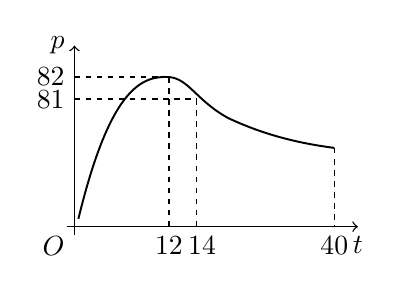
\begin{tikzpicture}[scale=1,line width=0.5pt]
\draw[->] (-0.1,0) -- (3.6,0) node[below] {$t$};
\draw[->] (0,-0.1) -- (0,2.3) node[left] {$p$};
\node[below left] at (0,0) {$O$};
\draw[line width=0.7pt] (0.05,0.1) .. controls (0.45,1.75) and (0.85,1.92) .. (1.2,1.9)
  .. controls (1.45,1.88) and (1.55,1.6) .. (1.95,1.38)
  .. controls (2.5,1.12) and (3.0,1.04) .. (3.3,1.0);
\draw[dash pattern=on 2pt off 2pt] (0,1.9) -- (1.2,1.9);
\draw[dash pattern=on 2pt off 2pt] (0,1.62) -- (1.55,1.62);
\draw[dash pattern=on 2pt off 2pt] (1.2,1.9) -- (1.2,0);
\draw[dash pattern=on 2pt off 2pt] (1.55,1.62) -- (1.55,0);
\draw[dash pattern=on 2pt off 2pt] (3.3,1.0) -- (3.3,0);
\node[left] at (0,1.9) {$82$};
\node[left] at (0,1.62) {$81$};
\node[below] at (1.2,0) {$12$};
\node[below] at (1.62,0) {$14$};
\node[below] at (3.3,0) {$40$};
\end{tikzpicture}
\end{center}

\ansspace*[12]

\ifanswer
\solbegin
\stepm{（1）}{由题意得当 $t\in(0,14]$ 时，设 $f(t)=c(t-12)^2+82$（$c<0$），}
\step{又 $f(14)=81$，所以 $c(14-12)^2+82=81$，解得 $c=-\dfrac14$；}
\step{所以 $f(t)=-\dfrac14(t-12)^2+82$,$t\in(0,14]$；}
\step{又当 $t\in[14,40]$ 时，函数 $y=\log_a(t-5)+83$（$a>0$ 且 $a\neq1$），}
\step{又当 $x=14$ 时，$y=81$，所以 $81=\log_a(14-5)+83$，解得 $a=\dfrac13$；}
\step{所以 $f(t)=\log_\frac13(t-5)+83$,$t\in[14,40]$，}
\step{所以 $p=\begin{cases}-\dfrac14(t-12)^2+82, & t\in(0,14]\\ \log_\frac13(t-5)+83, & t\in(14,40]\end{cases}$；}
\stepm{（2）}{当 $t=32$ 时，$p=\log_\frac13(32-5)+83=80$，}
\step{所以当一位学生在坚持听课 32 分钟时，注意力指数 $p$ 大约为 80；}
\stepm{（3）}{当 $t\in(0,14]$ 时，$-\dfrac14(t-12)^2+82\geqslant80$，解得 $t\in[12-2\sqrt2,14]$，}
\step{当 $t\in[14,40]$ 时，$\log_\frac13(t-5)+83\geqslant80$，解得 $5<t\leqslant32$，则 $t\in[14,32]$，}
\step{因此当 $t\in[12-2\sqrt2,32]$ 时学生听课效果最佳，}
\step{此时 $\Delta t=32-(12-2\sqrt2)=20+2\sqrt2>20$，}
\step{所以老师能经过合理安排时间在学生听课效果最佳时段讲完.}
\solend

\fi

\item 已知 $a\in R$，函数 $f(x+1)=\log_2\left(\dfrac{ax+1+a}{x+1}\right)$.

（1）若 $a=2$，求函数 $f(x)$ 的表达式及定义域；

（2）若关于 $x$ 的方程 $f\left(\dfrac x2\right)-\log_2[(a-2)x+3a-5]=0$ 的解集中恰好只有一个元素，求实
数 $a$ 的取值范围.

\ansspace*[14]

\ifanswer
\solbegin
\stepm{（1）}{$f(x+1)=\log_2\left(\dfrac{ax+1+a}{x+1}\right)$，}
\step{令 $x+1=t$，则 $f(t)=\log_2\left(\dfrac1t+a\right)$，即 $f(x)=\log_2\left(\dfrac1x+a\right)$，}
\step{因为 $a=2$，所以 $f(x)=\log_2\left(2+\dfrac1x\right)$，}
\step{由 $2+\dfrac1x>0$ 得定义域为 $\left(-\infty,-\dfrac12\right)\cup(0,+\infty)$；}
\stepm{（2）}{由（1）得 $f(x)=\log_2\left(\dfrac1x+a\right)$，}
\step{方程 $f\left(\dfrac x2\right)-\log_2[(a-2)x+3a-5]=0$，}
\step{即 $\log_2\left(\dfrac2x+a\right)-\log_2[(a-2)x+3a-5]=0$，}
\step{可转化为 $(a-2)x^2+(2a-5)x-2=0$，且 $\dfrac2x+a>0$.}
\step{①当 $a-2=0$，即 $a=2$ 时，$x=-2$，符合题意；}
\step{②当 $a-2\neq0$，即 $a\neq2$ 时，$x_1=-2$,$x_2=\dfrac1{a-2}$，}
\step{（$i$）当 $-2=\dfrac1{a-2}$ 时，即 $a=\dfrac32$ 时，符合题意；}
\step{（$ii$）当 $-2\neq\dfrac1{a-2}$ 时，即 $a\neq\dfrac32$ 且 $a\neq2$ 时，}
\step{要满足题意，则有 $\begin{cases}-1+a>0\\ 3a-4\leqslant0\end{cases}\Rightarrow1<a\leqslant\dfrac43$ 或 $\begin{cases}-1+a\leqslant0\\ 3a-4>0\end{cases}$，无解；}
\step{综上，$a$ 的取值范围 $\left(1,\dfrac43\right]\cup\left\{2,\dfrac32\right\}$.}
\solend

\fi

\item 已知函数 $y=f(x)$ 是定义在 $[0,+\infty)$ 上的函数，并且 $f(x)\geqslant0$，对于定义域内的任意自
变量的值 $x$、$y$，满足 $f(y)f(x^2f(y)+xf(y))=f(x^2+y+x)$，$f(a)=0$，其中
$a>0$.

（1）当 $f(0)\neq0$ 时，求 $f(0)$；

（2）已知当 $0\leqslant x<a$ 时，有 $f(x)\neq0$.

（$i$）求 $f(a+3)$；

（$ii$）求函数 $y=f(x)$ 的解析式（用 $a$ 表示）.

\ansspace*[16]

\ifanswer
\solbegin
\stepm{（1）}{因为 $f(x)\geqslant0$，且对于定义域内的任意自变量的值 $x$、$y$，}
\step{满足 $f(y)f(x^2f(y)+xf(y))=f(x^2+y+x)$，}
\step{令 $x=y=0$，则 $f^2(0)=f(0)$，因为 $f(0)\neq0$，所以 $f(0)=1$，}
\stepm{（2）}{（$i$）由 $f(y)f(x^2f(y)+xf(y))=f(x^2+y+x)$，}
\step{得 $f(y)f[(x^2+x)f(y)]=f[(x^2+x)+y]$，}
\step{令 $t=x^2+x$，因为 $x\geqslant0$，所以 $t=x^2+x\in[0,+\infty)$，}
\step{所以有 $f(y)f(tf(y))=f(t+y)$，因为 $f(a)=0$，}
\step{令 $y=a$，$t=3$，得 $f(a+3)=f(a)f(3f(a))=0\times f(3f(a))=0$；}
\step{（$ii$）当 $x\geqslant a$ 时，令 $y=a$，$t=x-a$，}
\step{$f(x)=f(x-a+a)=f(a)f[(x-a)f(a)]=0$.}
\step{当 $0\leqslant x<a$ 时，则有 $0<a-x\leqslant a$，令 $y=x$，$t=a-x$，}
\step{则 $f(a)=f(a-x+x)=f(x)f[(a-x)f(x)]=0$.}
\step{因为 $f(x)\neq0$，所以有 $f((a-x)f(x))=0$，则 $(a-x)f(x)\geqslant a$，}
\step{又因为 $a-x>0$，即 $f(x)\geqslant\dfrac a{a-x}$.}
\step{令 $t=\dfrac a{f(x)}>0$,$y=x>0$，}
\step{则 $f\left(\dfrac a{f(x)}+x\right)=f(x)\cdot f\left(\dfrac a{f(x)}\cdot f(x)\right)=f(x)\cdot f(a)=0$，}
\step{所以有 $\dfrac a{f(x)}+x\geqslant a$，即 $\dfrac a{f(x)}\geqslant a-x$，得 $f(x)\leqslant\dfrac a{a-x}$，}
\step{所以当 $0\leqslant x<a$ 时，$f(x)=\dfrac a{a-x}$.}
\step{综上，$f(x)=\begin{cases}\dfrac a{a-x}, & 0\leqslant x<a\\ 0, & x\geqslant a\end{cases}$.}
\solend

\fi

\end{enumerate}

\end{document}
"
% 紧凑版：xelatex "\def\iscompact{1}% 高一105_交附闵行_周末作业10.30.tex
%   —— 高一上数学“2026-2027 年交附闵行高一上周末作业 10.30”（试卷版/答案版）
% 试卷版：xelatex 高一105_交附闵行_周末作业10.30.tex
% 答案版：xelatex "\def\isanswer{1}\input{高一105_交附闵行_周末作业10.30.tex}"
% 紧凑版：xelatex "\def\iscompact{1}\input{高一105_交附闵行_周末作业10.30.tex}"
%
% 原始材料：微信公众号“魔都数学加油站”文章，作者破晓，2026-11-02 17:41 发布；
% 连载“27学年高一105”，原文标题“27学年高一105——2026-2027年上海市交附闵行高一上周末作业10.30”；
% 原文链接：https://mp.weixin.qq.com/s/XUfNEvGHjD0CB5jdoleBWw。
% 正文为 13 张 PNG 页（第 4、9、13 页 2560×3620，其余 4762×6735），题目下印有【解析】，为讲评版。
% 题目、解析均据原图转录；卷面水印及公众号页脚未录入。
%
% 卷首标题：原卷印作“2026-2027 年交附闵行高一上周末作业 10.30”（公众号标题中的“上海市”
% 卷面标题行没有，本稿照卷面），年份区间按全稿惯例排 en dash；原卷未印副标题，本稿按题目
% 内容标为“函数、不等式”（主体为指数与对数，第 3 题集合、第 16 题基本不等式）。
%
% 与原卷的排版差异：
%   ① 原文从第 3 题起，填空题编号为 3—12、选择题为 13—16、解答题为 17—21，本稿保留原题号；
%   ② 原卷每题下直接印【解析】，本稿按全稿惯例将解析置于答案版；选择题括号内未印答案，另由
%      解析末句“故选 X”给出；
%   ③ 原卷未印副标题，本稿按“知识模块”口径补出；
%   ④ 原卷填空横线按全稿惯例排为 \blankline[4.4em]；解答题按惯例加 \ansspace；选择题括号排
%      \mbox{（\quad）}、选项段前按惯例加 \keepwithprev；
%   ⑤ $f(x_1)_{max}$、$g(x)_max$、$\left(\frac{a+b+c}{b-a}\right)_{min}$ 等下标原卷排斜体，
%      按 高一96 成例改正体 $\max$、$\min$；
%   ⑥ 原卷数集排斜体 $R$／$Q$，按全稿惯例改 $\R$／$\Q$；
%   ⑦ 第 11 题解析的两幅三角形示意图与第 19 题题干的 $p$-$t$ 曲线图均按原图形状用 TikZ 重排
%      （第 19 题图属题干、三版都出；第 11 题图属解析、仅答案版显示）。
%
% 原卷存疑／笔误（均照录加注）：
%   第 14 题解析“但 $16=4^x=2^y=16$”（链首、链尾的两个 $16$ 系原卷笔误，按上下文应为
%   $4^x=2^y=16$）；
%   第 16 题选项的区间分隔逗号 A 项排半角、B／C／D 三项排全角（原卷自身不一致）；
%   第 21 题 (2) 的小问号排“（$i$）求…”（右括号紧贴“求”字），照录。
%
% 行数核对：逐题数 \step/\stepm 条数，合计 159 条（Q3：2；Q4：1；Q5：4；Q6：6；Q7：3；
% Q8：7；Q9：5；Q10：3；Q11：15；Q12：7；Q13：12；Q14：7；Q15：9；Q16：10；Q17：7；
% Q18：14；Q19：14；Q20：14；Q21：19），与原卷印刷行逐题相等。
%
\documentclass[a4paper,11pt]{article}
\usepackage{common}

\begin{document}

\examtitlest[3]{2026--2027 年交附闵行高一上周末作业 10.30}{函数、不等式}

\bigsec{一、填空题}

\begin{enumerate}
\setcounter{enumi}{2}

\item 已知集合 $M=\{1,m\}$，$N=\{n,\log_2n\}$，若 $M=N$，则 $(m-n)^{2027}=$\blankline[4.4em].

\ifanswer
\solbegin
\step{由题意得 $\begin{cases}n=1\\ \log_2n=m\end{cases}$ 或 $\begin{cases}n=m\\ \log_2n=1\end{cases}$，解得 $\begin{cases}n=1\\ m=0\end{cases}$ 或 $\begin{cases}n=2\\ m=2\end{cases}$，}
\step{所以 $(m-n)^{2027}=-1$ 或 $0$.}
\solend

\fi

\item 已知 $\log_{2x^2-1}(3x^2+2x-1)=1$，则 $x=$\blankline[4.4em].

\ifanswer
\solbegin
\step{因为 $\log_{2x^2-1}(3x^2+2x-1)=1$，所以 $\begin{cases}2x^2-1>0\\ 2x^2-1\neq1\\ 3x^2+2x-1>0\\ 2x^2-1=3x^2+2x-1\end{cases}$，解得 $x=-2$.}
\solend

\fi

\item 已知 $m>1$，$n>1$，$\lg m=\log_n100$，则 $mn$ 的最小值为\blankline[4.4em].

\ifanswer
\solbegin
\step{由 $m>1$，$n>1$，得 $\lg m>0$，$\lg n>0$，}
\step{因为 $\lg m=\log_n100=\dfrac{\lg100}{\lg n}=\dfrac2{\lg n}$，所以 $\lg m\cdot\lg n=2$，}
\step{所以 $\lg(mn)=\lg m+\lg n\geqslant2\sqrt{\lg m\cdot\lg n}=2\sqrt2$，}
\step{当且仅当 $m=n=10^{\sqrt2}$ 时取等号，则 $mn\geqslant10^{2\sqrt2}$，即 $mn$ 的最小值为 $10^{2\sqrt2}$.}
\solend

\fi

\item 设 $m$、$n$ 分别是方程 $\log_{2013}x+x-9=0$ 和 $2013^x+x-9=0$ 的根，则 $m+n=$\blankline[4.4em].

\ifanswer
\solbegin
\step{由 $\log_{2013}x+x-9=0$，得 $\log_{2013}x=-x+9$，}
\step{因为 $m$ 是方程 $\log_{2013}x+x-9=0$ 的根，}
\step{所以 $m$ 为函数 $y=\log_{2013}x$ 与 $y=-x+9$ 图象交点的横坐标，}
\step{同理 $n$ 是函数 $y=2013^x$ 与 $y=-x+9$ 图象交点的横坐标，}
\step{因为 $y=\log_{2013}x$ 与 $y=2013^x$ 互为反函数，其图象关于直线 $y=x$ 对称，}
\step{联立 $\begin{cases}y=-x+9\\ y=x\end{cases}$，解得 $x=\dfrac92$，所以 $m+n=\dfrac92\times2=9$.}
\solend

\fi

\item 已知函数 $f(x)=\dfrac1{\log_2(x^2+4)}$，则 $f(-2)=$\blankline[2em]，$f(x)$ 的值域为\blankline[4.4em].

\ifanswer
\solbegin
\step{$f(-2)=\dfrac1{\log_28}=\dfrac13$.}
\step{因为 $x^2+4\geqslant4$，所以 $\log_2(x^2+4)\geqslant\log_24=2$，所以 $0<\dfrac1{\log_2(x^2+4)}\leqslant\dfrac12$，}
\step{故 $f(x)$ 的值域为 $\left(0,\dfrac12\right]$.}
\solend

\fi

\item 已知 $\alpha$、$\beta$ 是方程 $9^x-2m\cdot3^x+m^2-1=0$ 的两个根，若 $\alpha+\beta=1$，则 $\alpha\beta=$\blankline[4.4em].

\ifanswer
\solbegin
\step{由题意得方程 $9^x-2m\cdot3^x+m^2-1=0$ 有两个根，}
\step{则方程 $t^2-2mt+m^2-1=0$ 有二正根，}
\step{则 $\begin{cases}\Delta=4m^2-4(m^2-1)\geqslant0\\ 2m>0\\ m^2-1>0\end{cases}$，解得 $m>1$，}
\step{又 $\alpha$、$\beta$ 是方程 $9^x-2m\cdot3^x+m^2-1=0$ 的两个根，}
\step{则 $3^\alpha\times3^\beta=m^2-1$，又 $\alpha+\beta=1$，则 $m^2-1=3^{\alpha+\beta}=3$，}
\step{解得 $m=2$ 或 $m=-2$（舍），则 $3^\alpha+3^\beta=2m=4$，又 $\alpha=1-\beta$，}
\step{则 $3^{1-\beta}+3^\beta=4$，解得 $\beta=0$ 或 $\beta=1$，则 $\begin{cases}\alpha=1\\ \beta=0\end{cases}$ 或 $\begin{cases}\alpha=0\\ \beta=1\end{cases}$，则 $\alpha\beta=0$.}
\solend

\fi

\item 已知 $a>b>0$，$\ln a=2\ln b$，且 $a\lg b=b\lg a$，则 $a+b=$\blankline[4.4em].

\ifanswer
\solbegin
\step{因为 $a>b>0$，$\ln a=2\ln b=\ln b^2$，所以 $a=b^2$，}
\step{由 $a\lg b=b\lg a$ 得 $b^2\lg b=b\lg b^2$，即 $b\lg b=2\lg b$，所以 $b=1$ 或 $b=2$，}
\step{当 $b=2$，$a=4$，满足题意，}
\step{当 $b=1$ 时，$a=1$ 与 $a>b>0$ 矛盾，所以 $b=1$ 舍去，}
\step{所以 $a+b=6$.}
\solend

\fi

\item 函数 $f(x)=\begin{cases}2^x, & x\leqslant t\\ \log_\frac12x, & x>t\end{cases}$ 的值域为 $M$，且 $8\notin M$，则实数 $t$ 的取值集合为\blankline[4.4em].

\ifanswer
\solbegin
\step{当 $x\leqslant t$ 时，函数 $f(x)=2^x$ 在 $(-\infty,t]$ 严格增，}
\step{当 $x>t$ 时，$f(x)=\log_\frac12x$ 在 $(t,+\infty)$ 严格减，}
\step{若 $8\notin M$，则满足条件 $\begin{cases}2^t<8\\ \log_\frac12t\leqslant8\end{cases}\Rightarrow\dfrac1{256}\leqslant t<3$，故实数 $t$ 的取值集合为 $\left[\dfrac1{256},3\right)$.}
\solend

\fi

\item 德国数学家狄利克雷在数学领域成就显著，以其命名函数 $D(x)=\begin{cases}1, & x\text{为有理数}\\ 0, & x\text{为无理数}\end{cases}$，该函
数被称为狄利克雷函数。那么是否存在三个点 $A(x_1,D(x_1))$、$B(x_2,D(x_2))$、$C(x_3,D(x_3))$，
使得 $\triangle ABC$ 为等边三角形，若不存在请在横线上填写“不存在”，如果存在则在横线上填写
该正三角形的面积\blankline[4.4em].

\ifanswer
\solbegin
\step{因为 $D(x)=\begin{cases}1, & x\text{为有理数}\\ 0, & x\text{为无理数}\end{cases}$，所以 $D(x)=0$ 或 1，}
\step{设存在三个点 $A(x_1,D(x_1))$、$B(x_2,D(x_2))$、$C(x_3,D(x_3))$，}
\step{使得 $\triangle ABC$ 为等边三角形，则 $D(x_1)$、$D(x_2)$、$D(x_3)$ 不同时为 0 或 1，}
\step{不妨设 $x_1<x_2<x_3$，分析得 $\triangle ABC$ 的位置有两种情况，}
\step{第一种情况：当 $x_1$ 为有理数时，即 $D(x_1)=1$，如图，过点 $B$ 作 $BD\perp AC$，}
\begin{center}
% 原图第 4 页解析示意图按原图形状用 TikZ 重排（第一种情况：$B$ 在 $x$ 轴上、$AC$ 在上方）。
\begin{tikzpicture}[scale=1,line width=0.5pt]
\draw (0,1.2) -- (2.6,1.2);
\node at (0.25,1.4) {$A$};
\node at (1.3,1.4) {$D$};
\node at (2.35,1.4) {$C$};
\draw[dash pattern=on 2pt off 2pt] (1.3,1.2) -- (1.3,0);
\draw (1.16,1.2) -- (1.16,1.06) -- (1.3,1.06);
\draw[->] (-0.5,0) -- (3.1,0) node[below] {$x$};
\node at (1.3,-0.24) {$B$};
\end{tikzpicture}
\end{center}
\step{垂足为 $D$，得 $BD=1$，$AD=\dfrac{\sqrt3}3$，$AB=AC=BC=\dfrac{2\sqrt3}3$，}
\step{则 $x_2=x_1+AD=x_1+\dfrac{\sqrt3}3$ 为无理数，$x_3=x_1+\dfrac{2\sqrt3}3$ 为无理数，}
\step{即 $D(x_2)=0$，$D(x_3)=0$ 与图形不一致，舍去；}
\step{第二种情况：当 $x_1$ 为无理数时，即 $D(x_1)=0$，如图，}
\step{过点 $B$ 作 $BD\perp AC$，垂足为 $D$，得 $BD=1$，$AD=\dfrac{\sqrt3}3$，}
\begin{center}
% 原图第 4 页解析示意图按原图形状用 TikZ 重排（第二种情况：$B$ 在上方、$AC$ 在 $x$ 轴上）。
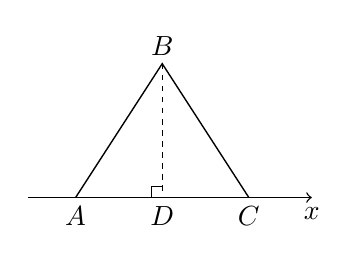
\begin{tikzpicture}[scale=1,line width=0.5pt]
\draw[->] (-0.4,0) -- (3.2,0) node[below] {$x$};
\draw (0.2,0) -- (1.3,1.7) -- (2.4,0);
\node at (0.2,-0.24) {$A$};
\node at (1.3,-0.24) {$D$};
\node at (2.4,-0.24) {$C$};
\node at (1.3,1.92) {$B$};
\draw[dash pattern=on 2pt off 2pt] (1.3,1.7) -- (1.3,0);
\draw (1.16,0) -- (1.16,0.14) -- (1.3,0.14);
\end{tikzpicture}
\end{center}
\step{$AB=AC=BC=\dfrac{2\sqrt3}3$，则 $x_2=x_1+AD=x_1+\dfrac{\sqrt3}3$，$x_3=x_1+\dfrac{2\sqrt3}3$，}
\step{存在 $x_1=-\dfrac{\sqrt3}3$，使得 $x_2=x_1+\dfrac{\sqrt3}3=0\in\Q$，且 $x_3=x_1+\dfrac{2\sqrt3}3=\dfrac{\sqrt3}3$ 为无理数，}
\step{即 $D(x_2)=1$，$D(x_3)=0$ 与图形一致，符合题意，}
\step{此时，$S_{\triangle ABC}=\dfrac12AC\cdot BD=\dfrac{\sqrt3}3$.}
\step{综上所述，存在这样的点 $A$、$B$、$C$，该正三角形的面积为 $\dfrac{\sqrt3}3$.}
\solend

\fi

\item 已知函数 $f(x)$ 满足：对 $\forall x\in R$，都有 $f(x+2025)\leqslant f(x)+2026$，
$f(x+2026)\geqslant f(x)+2027$，若 $f(1)=0$，则 $f(2)$ 的取值范围是\blankline[4.4em].

\ifanswer
\solbegin
\step{对 $\forall x\in R$，都有 $f(x+2025)\leqslant f(x)+2026$，$f(x+2026)\geqslant f(x)+2027$，}
\step{则 $f(x)+2027\leqslant f(x+2026)=f(x+1+2025)\leqslant f(x+1)+2026$，}
\step{即 $f(x)+1\leqslant f(x+1)$，所以 $f(2)\geqslant f(1)+1=1$；}
\step{$f(x)+2026\geqslant f(x+2025)=f(x+2024+1)\geqslant f(x+2024)+1$}
\step{$\geqslant\cdots\geqslant f(x+1)+2024$，所以 $f(x)+2\geqslant f(x+1)$，}
\step{所以 $f(2)\leqslant f(1)+2=2$；}
\step{即 $f(2)$ 的取值范围是 $[1,2]$.}
\solend

\fi

\end{enumerate}

\bigsec{二、选择题}

\begin{enumerate}
\setcounter{enumi}{12}

\item 若实数 $0<m<n<1$，而实数 $x>1$，则下列不等式正确的是\mbox{（\quad）}

\keepwithprev
A. $m^x<n^x$\qquad\qquad B. $x^m>x^n$\qquad\qquad C. $\log_xm>\log_xn$\qquad D. $\log_mx<\log_nx$

\ifanswer
\solbegin
\step{对于 $A$，函数 $f(t)=t^x$ 是以 $t$ 为变量，$x$ 为常量的幂函数，}
\step{由于 $x>1$，易得 $f(t)$ 在 $(0,+\infty)$ 上严格增，}
\step{$0<m<n<1$，$x>1$，可以得到 $m^x<n^x$，故 $A$ 正确；}
\step{对于 $B$，函数 $g(s)=x^s$，是以 $s$ 为变量，$x$ 为常量的指数函数，}
\step{由于 $x>1$，则 $g(s)$ 严格增，$0<m<n<1$，可以得到 $x^m<x^n$，故 $B$ 不正确；}
\step{对于 $C$，$\log_xm=\dfrac{\lg m}{\lg x}$，$\log_xn=\dfrac{\lg n}{\lg x}$，由于 $0<m<n<1$，则 $\lg m<\lg n<0$，}
\step{$x>1$，则 $\lg x>0$，则有 $\dfrac{\lg m}{\lg x}<\dfrac{\lg n}{\lg x}$，即 $\log_xm<\log_xn$，故 $C$ 不正确；}
\step{对于 $D$，由 $\log_mx-\log_nx=\dfrac{\lg x}{\lg m}-\dfrac{\lg x}{\lg n}=\dfrac{\lg x(\lg n-\lg m)}{\lg m\lg n}$，}
\step{因为实数 $0<m<n<1$，而实数 $x>1$，}
\step{所以 $\lg x>0$，$\lg m<\lg n<0$，则 $\dfrac{\lg x(\lg n-\lg m)}{\lg m\lg n}>0$，即 $\log_mx>\log_nx$，}
\step{故 $D$ 不正确.}
\step{故选 $A$.}
\solend

\fi

\item 已知 $x>1$，$y>1$，则 “$4^x>2^y$” 是 $\log_2x>\log_4(y-1)$ ”的\mbox{（\quad）}

\keepwithprev
A. 充分不必要条件\qquad\qquad B. 必要不充分条件

C. 充要条件\qquad\qquad D. 既不充分也不必要条件

\ifanswer
\solbegin
\step{因为 $x>1$，$y>1$，若 $4^x>2^y$，即 $2^{2x}>2^y$，所以 $2x>y>1$，}
\step{因为 $\dfrac y2-\sqrt{y-1}=\dfrac{(\sqrt{y-1})^2-2\sqrt{y-1}+1}2=\dfrac{(\sqrt{y-1}-1)^2}2\geqslant0$，}
\step{即 $\dfrac y2\geqslant\sqrt{y-1}>0$，所以 $\log_2\dfrac y2\geqslant\log_2\sqrt{y-1}=\dfrac12\log_2(y-1)=\log_4(y-1)$，}
\step{又 $x>\dfrac y2>\dfrac12$，所以 $\log_2x>\log_2\dfrac y2\geqslant\log_4(y-1)$，故充分性成立；}
\step{取 $x=2$，$y=4$，满足 $1=\log_2x>\log_4(y-1)=\log_43$，}
\step{但 $16=4^x=2^y=16$，即不满足 $4^x>2^y$，故必要性不成立.}% 链首链尾两个 16 系原卷笔误，应为 4^x=2^y=16，照录
\step{故选 $A$.}
\solend

\fi

\item 以下命题中，真命题的个数是\mbox{（\quad）}

①函数 $y=(x^2+1)^2+3$ 最小值为 3；②若 $2^a+\log_2a=4^b+2\log_4b$，则 $a<2b$；③不等式
$2^x-x-1>0$ 的解集为 $(1,+\infty)$.

\keepwithprev
A. $0$\qquad\qquad B. $1$\qquad\qquad C. $2$\qquad\qquad D. $3$

\ifanswer
\solbegin
\step{对于①，由于 $x^2+1\geqslant1$，则 $y=(x^2+1)^2+3\geqslant4$，}
\step{即函数 $y=(x^2+1)^2+3$ 最小值为 4，①错误；}
\step{对于②，由于 $b>0$，}
\step{则有 $2^a+\log_2a=4^b+2\log_4b=2^{2b}+\log_2b<2^{2b}+\log_22b$，}
\step{设 $f(x)=2^x+\log_2x$，易得 $f(x)$ 在 $(0,+\infty)$ 上为严格增函数，必有 $a<2b$，}
\step{②正确；}
\step{对于③，当 $x=-1$ 时，$2^x-x-1=2^x(x+1)>0$，即 $-1$ 在不等式的解集内，}
\step{③错误；}
\step{故选 $B$.}
\solend

\fi

\item 已知函数 $f(x)=ax^2+bx+c$（$a\neq0$ 且 $a<b$），若对任意的 $x\in R$，$f(x)\geqslant0$，且
$f(1)\geqslant\lambda(b-a)$，则实数 $\lambda$ 的取值范围为\mbox{（\quad）}

\keepwithprev
A. $(-\infty,2]$\qquad\qquad B. $[2\text{，}+\infty)$\qquad\qquad C. $(-\infty\text{，}3]$\qquad\qquad D. $[3\text{，}+\infty)$% 原卷 B/C/D 用全角逗号、A 用半角，照录

\ifanswer
\solbegin
\step{因为函数 $f(x)\geqslant0$ 恒成立，所以 $a>0$，且 $\Delta=b^2-4ac\leqslant0$，即 $c\geqslant\dfrac{b^2}{4a}$，}
\step{所以 $a+b+c\geqslant a+b+\dfrac{b^2}{4a}$，又 $a<b$，所以 $b-a>0$，}
\step{又 $f(1)\geqslant\lambda(b-a)$ 恒成立，所以 $a+b+c\geqslant\lambda(b-a)$ 恒成立，}
\step{即 $\lambda\leqslant\left(\dfrac{a+b+c}{b-a}\right)_{\min}=\dfrac{a+b+\dfrac{b^2}{4a}}{b-a}$，}
\step{令 $t=\dfrac ba$（$t>1$），则 $\dfrac{a+b+\dfrac{b^2}{4a}}{b-a}=\dfrac{1+t+\dfrac{t^2}4}{t-1}$，}
\step{令 $\mu=t-1$（$\mu>0$），则 $t=\mu+1$，}
\step{故上式 $=\dfrac{1+\mu+1+\dfrac{(\mu+1)^2}4}{\mu}=\dfrac14\left(\mu+\dfrac9\mu+6\right)$，}
\step{对 $\mu>0$，有 $\mu+\dfrac9\mu\geqslant2\sqrt{\mu\times\dfrac9\mu}=6$，当且仅当 $\mu=\dfrac9\mu$，即 $\mu=3$ 时取等号，}
\step{所以 $\dfrac14\left(\mu+\dfrac9\mu+6\right)\geqslant\dfrac14(6+6)=3$，故 $\lambda\leqslant3$，}
\step{即实数 $\lambda$ 的取值范围为 $(-\infty,3]$. 故选 $C$.}
\solend

\fi

\end{enumerate}

\bigsec{三、解答题}

\begin{enumerate}
\setcounter{enumi}{16}

\item 已知函数 $f(x)=\log_\frac23(ax^2-6x+18)$.

（1）若 $f(x)$ 的定义域为 $R$，求实数 $a$ 的取值范围.

（2）若 $f(x)$ 的值域为 $R$，求实数 $a$ 的取值范围.

\ansspace*[10]

\ifanswer
\solbegin
\stepm{（1）}{由 $f(x)=\log_\frac23(ax^2-6x+18)$ 的定义域为 $R$，得 $ax^2-6x+18>0$ 恒成立，}
\step{$a=0$ 时，$f(x)=\log_\frac23(18-6x)$ 的定义域为 $(-\infty,3)$，不符合题意.}
\step{$a\neq0$ 时，$\begin{cases}a>0\\ \Delta=36-4\times18a<0\end{cases}$，解得 $a>\dfrac12$.}
\step{综上，$a$ 的取值范围是 $\left(\dfrac12,+\infty\right)$.}
\stepm{（2）}{$a=0$ 时，$f(x)=\log_\frac23(18-6x)$ 的值域为 $R$，符合题意.}
\step{$a\neq0$ 时，$\begin{cases}a>0\\ \Delta=36-4\times18a\geqslant0\end{cases}$，解得 $0<a\leqslant\dfrac12$.}
\step{综上，$a$ 的取值范围是 $\left[0,\dfrac12\right]$.}
\solend

\fi

\item 已知 $f(x)=\log_ax+\log_a(6-x)$，$a>0$ 且 $a\neq1$，且 $f(3)=2$.

（1）求 $a$ 的值及 $f(x)$ 的单调区间.

（2）若对于 $\forall x_1\in(0,6)$，$\exists x_2\in[1,9]$，使得 $f(x_1)\leqslant t+\log_3x_2$ 成立，求实数 $t$ 的取值范
围.

\ansspace*[12]

\ifanswer
\solbegin
\stepm{（1）}{已知 $f(x)=\log_ax+\log_a(6-x)$，且 $f(3)=2$.}
\step{得 $\log_a3+\log_a(6-3)=2$，即 $2\log_a3=2$，}
\step{因此 $\log_a3=1$，因此 $a=3$，因此 $f(x)=\log_3x+\log_3(6-x)$，}
\step{因为 $\begin{cases}x>0\\ 6-x>0\end{cases}$，因此 $0<x<6$，故 $f(x)$ 的定义域为 $(0,6)$；}
\step{$f(x)=\log_3(6x-x^2)$，}
\step{因为函数 $y=6x-x^2$ 在 $(0,3)$ 上严格增，在 $(3,6)$ 上严格减，}
\step{又函数 $y=\log_3x$ 为严格增函数，}
\step{由复合函数的单调性得函数 $f(x)$ 在 $(0,3)$ 上严格增，在 $(3,6)$ 上严格减；}
\stepm{（2）}{令 $g(x)=t+\log_3x$，}
\step{因为 $\forall x_1\in(0,6)$，$\exists x_2\in[1,9]$，使得 $f(x_1)\leqslant t+\log_3x_2$，}
\step{即 $f(x_{1})_{\max}\leqslant g(x_{2})_{\max}$，}
\step{其中由（1）得 $f(x_{1})_{\max}=f(3)=2$.}
\step{又 $g(x)=t+\log_3x$ 在 $[1,9]$ 上严格增，因此 $g(x)_{\max}=g(9)=t+2$，}
\step{因此 $2\leqslant t+2$，因此实数 $t$ 的取值范围为 $[0,+\infty)$.}
\solend

\fi

\item 某心理学研究小组在对学生上课注意力集中情况的调查研究中，发现其注意力指数 $p$ 与
听课时间 $t$ 之间的关系满足如图所示的曲线. 当 $t\in(0,14]$ 时，曲线是二次函数图象的一部
分，当 $t\in[14,40]$ 时，曲线是函数 $y=\log_a(t-5)+83$（$a>0$ 且 $a\neq1$）图象的一部分. 根据
专家研究，当注意力指数 $p$ 大于等于 80 时听课效果最佳.

（1）试求 $p=f(t)$ 的函数关系式；

（2）当一位学生在坚持听课 32 分钟时，注意力指数 $p$ 大约为多少？

（3）一道数学难题，讲解需要 20 分钟，问老师能否经过合理安排在学生听
课效果最佳时讲完？请说明理由.

\begin{center}
% 原图第 9 页题干 p-t 曲线图按原图形状用 TikZ 重排（三版都出）。
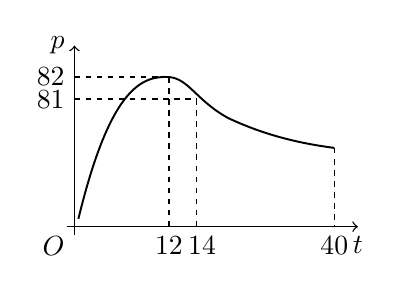
\begin{tikzpicture}[scale=1,line width=0.5pt]
\draw[->] (-0.1,0) -- (3.6,0) node[below] {$t$};
\draw[->] (0,-0.1) -- (0,2.3) node[left] {$p$};
\node[below left] at (0,0) {$O$};
\draw[line width=0.7pt] (0.05,0.1) .. controls (0.45,1.75) and (0.85,1.92) .. (1.2,1.9)
  .. controls (1.45,1.88) and (1.55,1.6) .. (1.95,1.38)
  .. controls (2.5,1.12) and (3.0,1.04) .. (3.3,1.0);
\draw[dash pattern=on 2pt off 2pt] (0,1.9) -- (1.2,1.9);
\draw[dash pattern=on 2pt off 2pt] (0,1.62) -- (1.55,1.62);
\draw[dash pattern=on 2pt off 2pt] (1.2,1.9) -- (1.2,0);
\draw[dash pattern=on 2pt off 2pt] (1.55,1.62) -- (1.55,0);
\draw[dash pattern=on 2pt off 2pt] (3.3,1.0) -- (3.3,0);
\node[left] at (0,1.9) {$82$};
\node[left] at (0,1.62) {$81$};
\node[below] at (1.2,0) {$12$};
\node[below] at (1.62,0) {$14$};
\node[below] at (3.3,0) {$40$};
\end{tikzpicture}
\end{center}

\ansspace*[12]

\ifanswer
\solbegin
\stepm{（1）}{由题意得当 $t\in(0,14]$ 时，设 $f(t)=c(t-12)^2+82$（$c<0$），}
\step{又 $f(14)=81$，所以 $c(14-12)^2+82=81$，解得 $c=-\dfrac14$；}
\step{所以 $f(t)=-\dfrac14(t-12)^2+82$,$t\in(0,14]$；}
\step{又当 $t\in[14,40]$ 时，函数 $y=\log_a(t-5)+83$（$a>0$ 且 $a\neq1$），}
\step{又当 $x=14$ 时，$y=81$，所以 $81=\log_a(14-5)+83$，解得 $a=\dfrac13$；}
\step{所以 $f(t)=\log_\frac13(t-5)+83$,$t\in[14,40]$，}
\step{所以 $p=\begin{cases}-\dfrac14(t-12)^2+82, & t\in(0,14]\\ \log_\frac13(t-5)+83, & t\in(14,40]\end{cases}$；}
\stepm{（2）}{当 $t=32$ 时，$p=\log_\frac13(32-5)+83=80$，}
\step{所以当一位学生在坚持听课 32 分钟时，注意力指数 $p$ 大约为 80；}
\stepm{（3）}{当 $t\in(0,14]$ 时，$-\dfrac14(t-12)^2+82\geqslant80$，解得 $t\in[12-2\sqrt2,14]$，}
\step{当 $t\in[14,40]$ 时，$\log_\frac13(t-5)+83\geqslant80$，解得 $5<t\leqslant32$，则 $t\in[14,32]$，}
\step{因此当 $t\in[12-2\sqrt2,32]$ 时学生听课效果最佳，}
\step{此时 $\Delta t=32-(12-2\sqrt2)=20+2\sqrt2>20$，}
\step{所以老师能经过合理安排时间在学生听课效果最佳时段讲完.}
\solend

\fi

\item 已知 $a\in R$，函数 $f(x+1)=\log_2\left(\dfrac{ax+1+a}{x+1}\right)$.

（1）若 $a=2$，求函数 $f(x)$ 的表达式及定义域；

（2）若关于 $x$ 的方程 $f\left(\dfrac x2\right)-\log_2[(a-2)x+3a-5]=0$ 的解集中恰好只有一个元素，求实
数 $a$ 的取值范围.

\ansspace*[14]

\ifanswer
\solbegin
\stepm{（1）}{$f(x+1)=\log_2\left(\dfrac{ax+1+a}{x+1}\right)$，}
\step{令 $x+1=t$，则 $f(t)=\log_2\left(\dfrac1t+a\right)$，即 $f(x)=\log_2\left(\dfrac1x+a\right)$，}
\step{因为 $a=2$，所以 $f(x)=\log_2\left(2+\dfrac1x\right)$，}
\step{由 $2+\dfrac1x>0$ 得定义域为 $\left(-\infty,-\dfrac12\right)\cup(0,+\infty)$；}
\stepm{（2）}{由（1）得 $f(x)=\log_2\left(\dfrac1x+a\right)$，}
\step{方程 $f\left(\dfrac x2\right)-\log_2[(a-2)x+3a-5]=0$，}
\step{即 $\log_2\left(\dfrac2x+a\right)-\log_2[(a-2)x+3a-5]=0$，}
\step{可转化为 $(a-2)x^2+(2a-5)x-2=0$，且 $\dfrac2x+a>0$.}
\step{①当 $a-2=0$，即 $a=2$ 时，$x=-2$，符合题意；}
\step{②当 $a-2\neq0$，即 $a\neq2$ 时，$x_1=-2$,$x_2=\dfrac1{a-2}$，}
\step{（$i$）当 $-2=\dfrac1{a-2}$ 时，即 $a=\dfrac32$ 时，符合题意；}
\step{（$ii$）当 $-2\neq\dfrac1{a-2}$ 时，即 $a\neq\dfrac32$ 且 $a\neq2$ 时，}
\step{要满足题意，则有 $\begin{cases}-1+a>0\\ 3a-4\leqslant0\end{cases}\Rightarrow1<a\leqslant\dfrac43$ 或 $\begin{cases}-1+a\leqslant0\\ 3a-4>0\end{cases}$，无解；}
\step{综上，$a$ 的取值范围 $\left(1,\dfrac43\right]\cup\left\{2,\dfrac32\right\}$.}
\solend

\fi

\item 已知函数 $y=f(x)$ 是定义在 $[0,+\infty)$ 上的函数，并且 $f(x)\geqslant0$，对于定义域内的任意自
变量的值 $x$、$y$，满足 $f(y)f(x^2f(y)+xf(y))=f(x^2+y+x)$，$f(a)=0$，其中
$a>0$.

（1）当 $f(0)\neq0$ 时，求 $f(0)$；

（2）已知当 $0\leqslant x<a$ 时，有 $f(x)\neq0$.

（$i$）求 $f(a+3)$；

（$ii$）求函数 $y=f(x)$ 的解析式（用 $a$ 表示）.

\ansspace*[16]

\ifanswer
\solbegin
\stepm{（1）}{因为 $f(x)\geqslant0$，且对于定义域内的任意自变量的值 $x$、$y$，}
\step{满足 $f(y)f(x^2f(y)+xf(y))=f(x^2+y+x)$，}
\step{令 $x=y=0$，则 $f^2(0)=f(0)$，因为 $f(0)\neq0$，所以 $f(0)=1$，}
\stepm{（2）}{（$i$）由 $f(y)f(x^2f(y)+xf(y))=f(x^2+y+x)$，}
\step{得 $f(y)f[(x^2+x)f(y)]=f[(x^2+x)+y]$，}
\step{令 $t=x^2+x$，因为 $x\geqslant0$，所以 $t=x^2+x\in[0,+\infty)$，}
\step{所以有 $f(y)f(tf(y))=f(t+y)$，因为 $f(a)=0$，}
\step{令 $y=a$，$t=3$，得 $f(a+3)=f(a)f(3f(a))=0\times f(3f(a))=0$；}
\step{（$ii$）当 $x\geqslant a$ 时，令 $y=a$，$t=x-a$，}
\step{$f(x)=f(x-a+a)=f(a)f[(x-a)f(a)]=0$.}
\step{当 $0\leqslant x<a$ 时，则有 $0<a-x\leqslant a$，令 $y=x$，$t=a-x$，}
\step{则 $f(a)=f(a-x+x)=f(x)f[(a-x)f(x)]=0$.}
\step{因为 $f(x)\neq0$，所以有 $f((a-x)f(x))=0$，则 $(a-x)f(x)\geqslant a$，}
\step{又因为 $a-x>0$，即 $f(x)\geqslant\dfrac a{a-x}$.}
\step{令 $t=\dfrac a{f(x)}>0$,$y=x>0$，}
\step{则 $f\left(\dfrac a{f(x)}+x\right)=f(x)\cdot f\left(\dfrac a{f(x)}\cdot f(x)\right)=f(x)\cdot f(a)=0$，}
\step{所以有 $\dfrac a{f(x)}+x\geqslant a$，即 $\dfrac a{f(x)}\geqslant a-x$，得 $f(x)\leqslant\dfrac a{a-x}$，}
\step{所以当 $0\leqslant x<a$ 时，$f(x)=\dfrac a{a-x}$.}
\step{综上，$f(x)=\begin{cases}\dfrac a{a-x}, & 0\leqslant x<a\\ 0, & x\geqslant a\end{cases}$.}
\solend

\fi

\end{enumerate}

\end{document}
"
%
% 原始材料：微信公众号“魔都数学加油站”文章，作者破晓，2026-11-02 17:41 发布；
% 连载“27学年高一105”，原文标题“27学年高一105——2026-2027年上海市交附闵行高一上周末作业10.30”；
% 原文链接：https://mp.weixin.qq.com/s/XUfNEvGHjD0CB5jdoleBWw。
% 正文为 13 张 PNG 页（第 4、9、13 页 2560×3620，其余 4762×6735），题目下印有【解析】，为讲评版。
% 题目、解析均据原图转录；卷面水印及公众号页脚未录入。
%
% 卷首标题：原卷印作“2026-2027 年交附闵行高一上周末作业 10.30”（公众号标题中的“上海市”
% 卷面标题行没有，本稿照卷面），年份区间按全稿惯例排 en dash；原卷未印副标题，本稿按题目
% 内容标为“函数、不等式”（主体为指数与对数，第 3 题集合、第 16 题基本不等式）。
%
% 与原卷的排版差异：
%   ① 原文从第 3 题起，填空题编号为 3—12、选择题为 13—16、解答题为 17—21，本稿保留原题号；
%   ② 原卷每题下直接印【解析】，本稿按全稿惯例将解析置于答案版；选择题括号内未印答案，另由
%      解析末句“故选 X”给出；
%   ③ 原卷未印副标题，本稿按“知识模块”口径补出；
%   ④ 原卷填空横线按全稿惯例排为 \blankline[4.4em]；解答题按惯例加 \ansspace；选择题括号排
%      \mbox{（\quad）}、选项段前按惯例加 \keepwithprev；
%   ⑤ $f(x_1)_{max}$、$g(x)_max$、$\left(\frac{a+b+c}{b-a}\right)_{min}$ 等下标原卷排斜体，
%      按 高一96 成例改正体 $\max$、$\min$；
%   ⑥ 原卷数集排斜体 $R$／$Q$，按全稿惯例改 $\R$／$\Q$；
%   ⑦ 第 11 题解析的两幅三角形示意图与第 19 题题干的 $p$-$t$ 曲线图均按原图形状用 TikZ 重排
%      （第 19 题图属题干、三版都出；第 11 题图属解析、仅答案版显示）。
%
% 原卷存疑／笔误（均照录加注）：
%   第 14 题解析“但 $16=4^x=2^y=16$”（链首、链尾的两个 $16$ 系原卷笔误，按上下文应为
%   $4^x=2^y=16$）；
%   第 16 题选项的区间分隔逗号 A 项排半角、B／C／D 三项排全角（原卷自身不一致）；
%   第 21 题 (2) 的小问号排“（$i$）求…”（右括号紧贴“求”字），照录。
%
% 行数核对：逐题数 \step/\stepm 条数，合计 159 条（Q3：2；Q4：1；Q5：4；Q6：6；Q7：3；
% Q8：7；Q9：5；Q10：3；Q11：15；Q12：7；Q13：12；Q14：7；Q15：9；Q16：10；Q17：7；
% Q18：14；Q19：14；Q20：14；Q21：19），与原卷印刷行逐题相等。
%
\documentclass[a4paper,11pt]{article}
\usepackage{common}

\begin{document}

\examtitlest[3]{2026--2027 年交附闵行高一上周末作业 10.30}{函数、不等式}

\bigsec{一、填空题}

\begin{enumerate}
\setcounter{enumi}{2}

\item 已知集合 $M=\{1,m\}$，$N=\{n,\log_2n\}$，若 $M=N$，则 $(m-n)^{2027}=$\blankline[4.4em].

\ifanswer
\solbegin
\step{由题意得 $\begin{cases}n=1\\ \log_2n=m\end{cases}$ 或 $\begin{cases}n=m\\ \log_2n=1\end{cases}$，解得 $\begin{cases}n=1\\ m=0\end{cases}$ 或 $\begin{cases}n=2\\ m=2\end{cases}$，}
\step{所以 $(m-n)^{2027}=-1$ 或 $0$.}
\solend

\fi

\item 已知 $\log_{2x^2-1}(3x^2+2x-1)=1$，则 $x=$\blankline[4.4em].

\ifanswer
\solbegin
\step{因为 $\log_{2x^2-1}(3x^2+2x-1)=1$，所以 $\begin{cases}2x^2-1>0\\ 2x^2-1\neq1\\ 3x^2+2x-1>0\\ 2x^2-1=3x^2+2x-1\end{cases}$，解得 $x=-2$.}
\solend

\fi

\item 已知 $m>1$，$n>1$，$\lg m=\log_n100$，则 $mn$ 的最小值为\blankline[4.4em].

\ifanswer
\solbegin
\step{由 $m>1$，$n>1$，得 $\lg m>0$，$\lg n>0$，}
\step{因为 $\lg m=\log_n100=\dfrac{\lg100}{\lg n}=\dfrac2{\lg n}$，所以 $\lg m\cdot\lg n=2$，}
\step{所以 $\lg(mn)=\lg m+\lg n\geqslant2\sqrt{\lg m\cdot\lg n}=2\sqrt2$，}
\step{当且仅当 $m=n=10^{\sqrt2}$ 时取等号，则 $mn\geqslant10^{2\sqrt2}$，即 $mn$ 的最小值为 $10^{2\sqrt2}$.}
\solend

\fi

\item 设 $m$、$n$ 分别是方程 $\log_{2013}x+x-9=0$ 和 $2013^x+x-9=0$ 的根，则 $m+n=$\blankline[4.4em].

\ifanswer
\solbegin
\step{由 $\log_{2013}x+x-9=0$，得 $\log_{2013}x=-x+9$，}
\step{因为 $m$ 是方程 $\log_{2013}x+x-9=0$ 的根，}
\step{所以 $m$ 为函数 $y=\log_{2013}x$ 与 $y=-x+9$ 图象交点的横坐标，}
\step{同理 $n$ 是函数 $y=2013^x$ 与 $y=-x+9$ 图象交点的横坐标，}
\step{因为 $y=\log_{2013}x$ 与 $y=2013^x$ 互为反函数，其图象关于直线 $y=x$ 对称，}
\step{联立 $\begin{cases}y=-x+9\\ y=x\end{cases}$，解得 $x=\dfrac92$，所以 $m+n=\dfrac92\times2=9$.}
\solend

\fi

\item 已知函数 $f(x)=\dfrac1{\log_2(x^2+4)}$，则 $f(-2)=$\blankline[2em]，$f(x)$ 的值域为\blankline[4.4em].

\ifanswer
\solbegin
\step{$f(-2)=\dfrac1{\log_28}=\dfrac13$.}
\step{因为 $x^2+4\geqslant4$，所以 $\log_2(x^2+4)\geqslant\log_24=2$，所以 $0<\dfrac1{\log_2(x^2+4)}\leqslant\dfrac12$，}
\step{故 $f(x)$ 的值域为 $\left(0,\dfrac12\right]$.}
\solend

\fi

\item 已知 $\alpha$、$\beta$ 是方程 $9^x-2m\cdot3^x+m^2-1=0$ 的两个根，若 $\alpha+\beta=1$，则 $\alpha\beta=$\blankline[4.4em].

\ifanswer
\solbegin
\step{由题意得方程 $9^x-2m\cdot3^x+m^2-1=0$ 有两个根，}
\step{则方程 $t^2-2mt+m^2-1=0$ 有二正根，}
\step{则 $\begin{cases}\Delta=4m^2-4(m^2-1)\geqslant0\\ 2m>0\\ m^2-1>0\end{cases}$，解得 $m>1$，}
\step{又 $\alpha$、$\beta$ 是方程 $9^x-2m\cdot3^x+m^2-1=0$ 的两个根，}
\step{则 $3^\alpha\times3^\beta=m^2-1$，又 $\alpha+\beta=1$，则 $m^2-1=3^{\alpha+\beta}=3$，}
\step{解得 $m=2$ 或 $m=-2$（舍），则 $3^\alpha+3^\beta=2m=4$，又 $\alpha=1-\beta$，}
\step{则 $3^{1-\beta}+3^\beta=4$，解得 $\beta=0$ 或 $\beta=1$，则 $\begin{cases}\alpha=1\\ \beta=0\end{cases}$ 或 $\begin{cases}\alpha=0\\ \beta=1\end{cases}$，则 $\alpha\beta=0$.}
\solend

\fi

\item 已知 $a>b>0$，$\ln a=2\ln b$，且 $a\lg b=b\lg a$，则 $a+b=$\blankline[4.4em].

\ifanswer
\solbegin
\step{因为 $a>b>0$，$\ln a=2\ln b=\ln b^2$，所以 $a=b^2$，}
\step{由 $a\lg b=b\lg a$ 得 $b^2\lg b=b\lg b^2$，即 $b\lg b=2\lg b$，所以 $b=1$ 或 $b=2$，}
\step{当 $b=2$，$a=4$，满足题意，}
\step{当 $b=1$ 时，$a=1$ 与 $a>b>0$ 矛盾，所以 $b=1$ 舍去，}
\step{所以 $a+b=6$.}
\solend

\fi

\item 函数 $f(x)=\begin{cases}2^x, & x\leqslant t\\ \log_\frac12x, & x>t\end{cases}$ 的值域为 $M$，且 $8\notin M$，则实数 $t$ 的取值集合为\blankline[4.4em].

\ifanswer
\solbegin
\step{当 $x\leqslant t$ 时，函数 $f(x)=2^x$ 在 $(-\infty,t]$ 严格增，}
\step{当 $x>t$ 时，$f(x)=\log_\frac12x$ 在 $(t,+\infty)$ 严格减，}
\step{若 $8\notin M$，则满足条件 $\begin{cases}2^t<8\\ \log_\frac12t\leqslant8\end{cases}\Rightarrow\dfrac1{256}\leqslant t<3$，故实数 $t$ 的取值集合为 $\left[\dfrac1{256},3\right)$.}
\solend

\fi

\item 德国数学家狄利克雷在数学领域成就显著，以其命名函数 $D(x)=\begin{cases}1, & x\text{为有理数}\\ 0, & x\text{为无理数}\end{cases}$，该函
数被称为狄利克雷函数。那么是否存在三个点 $A(x_1,D(x_1))$、$B(x_2,D(x_2))$、$C(x_3,D(x_3))$，
使得 $\triangle ABC$ 为等边三角形，若不存在请在横线上填写“不存在”，如果存在则在横线上填写
该正三角形的面积\blankline[4.4em].

\ifanswer
\solbegin
\step{因为 $D(x)=\begin{cases}1, & x\text{为有理数}\\ 0, & x\text{为无理数}\end{cases}$，所以 $D(x)=0$ 或 1，}
\step{设存在三个点 $A(x_1,D(x_1))$、$B(x_2,D(x_2))$、$C(x_3,D(x_3))$，}
\step{使得 $\triangle ABC$ 为等边三角形，则 $D(x_1)$、$D(x_2)$、$D(x_3)$ 不同时为 0 或 1，}
\step{不妨设 $x_1<x_2<x_3$，分析得 $\triangle ABC$ 的位置有两种情况，}
\step{第一种情况：当 $x_1$ 为有理数时，即 $D(x_1)=1$，如图，过点 $B$ 作 $BD\perp AC$，}
\begin{center}
% 原图第 4 页解析示意图按原图形状用 TikZ 重排（第一种情况：$B$ 在 $x$ 轴上、$AC$ 在上方）。
\begin{tikzpicture}[scale=1,line width=0.5pt]
\draw (0,1.2) -- (2.6,1.2);
\node at (0.25,1.4) {$A$};
\node at (1.3,1.4) {$D$};
\node at (2.35,1.4) {$C$};
\draw[dash pattern=on 2pt off 2pt] (1.3,1.2) -- (1.3,0);
\draw (1.16,1.2) -- (1.16,1.06) -- (1.3,1.06);
\draw[->] (-0.5,0) -- (3.1,0) node[below] {$x$};
\node at (1.3,-0.24) {$B$};
\end{tikzpicture}
\end{center}
\step{垂足为 $D$，得 $BD=1$，$AD=\dfrac{\sqrt3}3$，$AB=AC=BC=\dfrac{2\sqrt3}3$，}
\step{则 $x_2=x_1+AD=x_1+\dfrac{\sqrt3}3$ 为无理数，$x_3=x_1+\dfrac{2\sqrt3}3$ 为无理数，}
\step{即 $D(x_2)=0$，$D(x_3)=0$ 与图形不一致，舍去；}
\step{第二种情况：当 $x_1$ 为无理数时，即 $D(x_1)=0$，如图，}
\step{过点 $B$ 作 $BD\perp AC$，垂足为 $D$，得 $BD=1$，$AD=\dfrac{\sqrt3}3$，}
\begin{center}
% 原图第 4 页解析示意图按原图形状用 TikZ 重排（第二种情况：$B$ 在上方、$AC$ 在 $x$ 轴上）。
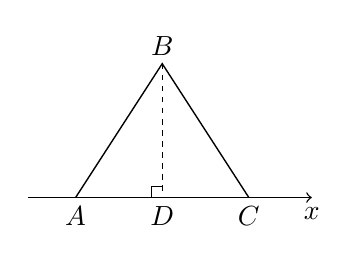
\begin{tikzpicture}[scale=1,line width=0.5pt]
\draw[->] (-0.4,0) -- (3.2,0) node[below] {$x$};
\draw (0.2,0) -- (1.3,1.7) -- (2.4,0);
\node at (0.2,-0.24) {$A$};
\node at (1.3,-0.24) {$D$};
\node at (2.4,-0.24) {$C$};
\node at (1.3,1.92) {$B$};
\draw[dash pattern=on 2pt off 2pt] (1.3,1.7) -- (1.3,0);
\draw (1.16,0) -- (1.16,0.14) -- (1.3,0.14);
\end{tikzpicture}
\end{center}
\step{$AB=AC=BC=\dfrac{2\sqrt3}3$，则 $x_2=x_1+AD=x_1+\dfrac{\sqrt3}3$，$x_3=x_1+\dfrac{2\sqrt3}3$，}
\step{存在 $x_1=-\dfrac{\sqrt3}3$，使得 $x_2=x_1+\dfrac{\sqrt3}3=0\in\Q$，且 $x_3=x_1+\dfrac{2\sqrt3}3=\dfrac{\sqrt3}3$ 为无理数，}
\step{即 $D(x_2)=1$，$D(x_3)=0$ 与图形一致，符合题意，}
\step{此时，$S_{\triangle ABC}=\dfrac12AC\cdot BD=\dfrac{\sqrt3}3$.}
\step{综上所述，存在这样的点 $A$、$B$、$C$，该正三角形的面积为 $\dfrac{\sqrt3}3$.}
\solend

\fi

\item 已知函数 $f(x)$ 满足：对 $\forall x\in R$，都有 $f(x+2025)\leqslant f(x)+2026$，
$f(x+2026)\geqslant f(x)+2027$，若 $f(1)=0$，则 $f(2)$ 的取值范围是\blankline[4.4em].

\ifanswer
\solbegin
\step{对 $\forall x\in R$，都有 $f(x+2025)\leqslant f(x)+2026$，$f(x+2026)\geqslant f(x)+2027$，}
\step{则 $f(x)+2027\leqslant f(x+2026)=f(x+1+2025)\leqslant f(x+1)+2026$，}
\step{即 $f(x)+1\leqslant f(x+1)$，所以 $f(2)\geqslant f(1)+1=1$；}
\step{$f(x)+2026\geqslant f(x+2025)=f(x+2024+1)\geqslant f(x+2024)+1$}
\step{$\geqslant\cdots\geqslant f(x+1)+2024$，所以 $f(x)+2\geqslant f(x+1)$，}
\step{所以 $f(2)\leqslant f(1)+2=2$；}
\step{即 $f(2)$ 的取值范围是 $[1,2]$.}
\solend

\fi

\end{enumerate}

\bigsec{二、选择题}

\begin{enumerate}
\setcounter{enumi}{12}

\item 若实数 $0<m<n<1$，而实数 $x>1$，则下列不等式正确的是\mbox{（\quad）}

\keepwithprev
A. $m^x<n^x$\qquad\qquad B. $x^m>x^n$\qquad\qquad C. $\log_xm>\log_xn$\qquad D. $\log_mx<\log_nx$

\ifanswer
\solbegin
\step{对于 $A$，函数 $f(t)=t^x$ 是以 $t$ 为变量，$x$ 为常量的幂函数，}
\step{由于 $x>1$，易得 $f(t)$ 在 $(0,+\infty)$ 上严格增，}
\step{$0<m<n<1$，$x>1$，可以得到 $m^x<n^x$，故 $A$ 正确；}
\step{对于 $B$，函数 $g(s)=x^s$，是以 $s$ 为变量，$x$ 为常量的指数函数，}
\step{由于 $x>1$，则 $g(s)$ 严格增，$0<m<n<1$，可以得到 $x^m<x^n$，故 $B$ 不正确；}
\step{对于 $C$，$\log_xm=\dfrac{\lg m}{\lg x}$，$\log_xn=\dfrac{\lg n}{\lg x}$，由于 $0<m<n<1$，则 $\lg m<\lg n<0$，}
\step{$x>1$，则 $\lg x>0$，则有 $\dfrac{\lg m}{\lg x}<\dfrac{\lg n}{\lg x}$，即 $\log_xm<\log_xn$，故 $C$ 不正确；}
\step{对于 $D$，由 $\log_mx-\log_nx=\dfrac{\lg x}{\lg m}-\dfrac{\lg x}{\lg n}=\dfrac{\lg x(\lg n-\lg m)}{\lg m\lg n}$，}
\step{因为实数 $0<m<n<1$，而实数 $x>1$，}
\step{所以 $\lg x>0$，$\lg m<\lg n<0$，则 $\dfrac{\lg x(\lg n-\lg m)}{\lg m\lg n}>0$，即 $\log_mx>\log_nx$，}
\step{故 $D$ 不正确.}
\step{故选 $A$.}
\solend

\fi

\item 已知 $x>1$，$y>1$，则 “$4^x>2^y$” 是 $\log_2x>\log_4(y-1)$ ”的\mbox{（\quad）}

\keepwithprev
A. 充分不必要条件\qquad\qquad B. 必要不充分条件

C. 充要条件\qquad\qquad D. 既不充分也不必要条件

\ifanswer
\solbegin
\step{因为 $x>1$，$y>1$，若 $4^x>2^y$，即 $2^{2x}>2^y$，所以 $2x>y>1$，}
\step{因为 $\dfrac y2-\sqrt{y-1}=\dfrac{(\sqrt{y-1})^2-2\sqrt{y-1}+1}2=\dfrac{(\sqrt{y-1}-1)^2}2\geqslant0$，}
\step{即 $\dfrac y2\geqslant\sqrt{y-1}>0$，所以 $\log_2\dfrac y2\geqslant\log_2\sqrt{y-1}=\dfrac12\log_2(y-1)=\log_4(y-1)$，}
\step{又 $x>\dfrac y2>\dfrac12$，所以 $\log_2x>\log_2\dfrac y2\geqslant\log_4(y-1)$，故充分性成立；}
\step{取 $x=2$，$y=4$，满足 $1=\log_2x>\log_4(y-1)=\log_43$，}
\step{但 $16=4^x=2^y=16$，即不满足 $4^x>2^y$，故必要性不成立.}% 链首链尾两个 16 系原卷笔误，应为 4^x=2^y=16，照录
\step{故选 $A$.}
\solend

\fi

\item 以下命题中，真命题的个数是\mbox{（\quad）}

①函数 $y=(x^2+1)^2+3$ 最小值为 3；②若 $2^a+\log_2a=4^b+2\log_4b$，则 $a<2b$；③不等式
$2^x-x-1>0$ 的解集为 $(1,+\infty)$.

\keepwithprev
A. $0$\qquad\qquad B. $1$\qquad\qquad C. $2$\qquad\qquad D. $3$

\ifanswer
\solbegin
\step{对于①，由于 $x^2+1\geqslant1$，则 $y=(x^2+1)^2+3\geqslant4$，}
\step{即函数 $y=(x^2+1)^2+3$ 最小值为 4，①错误；}
\step{对于②，由于 $b>0$，}
\step{则有 $2^a+\log_2a=4^b+2\log_4b=2^{2b}+\log_2b<2^{2b}+\log_22b$，}
\step{设 $f(x)=2^x+\log_2x$，易得 $f(x)$ 在 $(0,+\infty)$ 上为严格增函数，必有 $a<2b$，}
\step{②正确；}
\step{对于③，当 $x=-1$ 时，$2^x-x-1=2^x(x+1)>0$，即 $-1$ 在不等式的解集内，}
\step{③错误；}
\step{故选 $B$.}
\solend

\fi

\item 已知函数 $f(x)=ax^2+bx+c$（$a\neq0$ 且 $a<b$），若对任意的 $x\in R$，$f(x)\geqslant0$，且
$f(1)\geqslant\lambda(b-a)$，则实数 $\lambda$ 的取值范围为\mbox{（\quad）}

\keepwithprev
A. $(-\infty,2]$\qquad\qquad B. $[2\text{，}+\infty)$\qquad\qquad C. $(-\infty\text{，}3]$\qquad\qquad D. $[3\text{，}+\infty)$% 原卷 B/C/D 用全角逗号、A 用半角，照录

\ifanswer
\solbegin
\step{因为函数 $f(x)\geqslant0$ 恒成立，所以 $a>0$，且 $\Delta=b^2-4ac\leqslant0$，即 $c\geqslant\dfrac{b^2}{4a}$，}
\step{所以 $a+b+c\geqslant a+b+\dfrac{b^2}{4a}$，又 $a<b$，所以 $b-a>0$，}
\step{又 $f(1)\geqslant\lambda(b-a)$ 恒成立，所以 $a+b+c\geqslant\lambda(b-a)$ 恒成立，}
\step{即 $\lambda\leqslant\left(\dfrac{a+b+c}{b-a}\right)_{\min}=\dfrac{a+b+\dfrac{b^2}{4a}}{b-a}$，}
\step{令 $t=\dfrac ba$（$t>1$），则 $\dfrac{a+b+\dfrac{b^2}{4a}}{b-a}=\dfrac{1+t+\dfrac{t^2}4}{t-1}$，}
\step{令 $\mu=t-1$（$\mu>0$），则 $t=\mu+1$，}
\step{故上式 $=\dfrac{1+\mu+1+\dfrac{(\mu+1)^2}4}{\mu}=\dfrac14\left(\mu+\dfrac9\mu+6\right)$，}
\step{对 $\mu>0$，有 $\mu+\dfrac9\mu\geqslant2\sqrt{\mu\times\dfrac9\mu}=6$，当且仅当 $\mu=\dfrac9\mu$，即 $\mu=3$ 时取等号，}
\step{所以 $\dfrac14\left(\mu+\dfrac9\mu+6\right)\geqslant\dfrac14(6+6)=3$，故 $\lambda\leqslant3$，}
\step{即实数 $\lambda$ 的取值范围为 $(-\infty,3]$. 故选 $C$.}
\solend

\fi

\end{enumerate}

\bigsec{三、解答题}

\begin{enumerate}
\setcounter{enumi}{16}

\item 已知函数 $f(x)=\log_\frac23(ax^2-6x+18)$.

（1）若 $f(x)$ 的定义域为 $R$，求实数 $a$ 的取值范围.

（2）若 $f(x)$ 的值域为 $R$，求实数 $a$ 的取值范围.

\ansspace*[10]

\ifanswer
\solbegin
\stepm{（1）}{由 $f(x)=\log_\frac23(ax^2-6x+18)$ 的定义域为 $R$，得 $ax^2-6x+18>0$ 恒成立，}
\step{$a=0$ 时，$f(x)=\log_\frac23(18-6x)$ 的定义域为 $(-\infty,3)$，不符合题意.}
\step{$a\neq0$ 时，$\begin{cases}a>0\\ \Delta=36-4\times18a<0\end{cases}$，解得 $a>\dfrac12$.}
\step{综上，$a$ 的取值范围是 $\left(\dfrac12,+\infty\right)$.}
\stepm{（2）}{$a=0$ 时，$f(x)=\log_\frac23(18-6x)$ 的值域为 $R$，符合题意.}
\step{$a\neq0$ 时，$\begin{cases}a>0\\ \Delta=36-4\times18a\geqslant0\end{cases}$，解得 $0<a\leqslant\dfrac12$.}
\step{综上，$a$ 的取值范围是 $\left[0,\dfrac12\right]$.}
\solend

\fi

\item 已知 $f(x)=\log_ax+\log_a(6-x)$，$a>0$ 且 $a\neq1$，且 $f(3)=2$.

（1）求 $a$ 的值及 $f(x)$ 的单调区间.

（2）若对于 $\forall x_1\in(0,6)$，$\exists x_2\in[1,9]$，使得 $f(x_1)\leqslant t+\log_3x_2$ 成立，求实数 $t$ 的取值范
围.

\ansspace*[12]

\ifanswer
\solbegin
\stepm{（1）}{已知 $f(x)=\log_ax+\log_a(6-x)$，且 $f(3)=2$.}
\step{得 $\log_a3+\log_a(6-3)=2$，即 $2\log_a3=2$，}
\step{因此 $\log_a3=1$，因此 $a=3$，因此 $f(x)=\log_3x+\log_3(6-x)$，}
\step{因为 $\begin{cases}x>0\\ 6-x>0\end{cases}$，因此 $0<x<6$，故 $f(x)$ 的定义域为 $(0,6)$；}
\step{$f(x)=\log_3(6x-x^2)$，}
\step{因为函数 $y=6x-x^2$ 在 $(0,3)$ 上严格增，在 $(3,6)$ 上严格减，}
\step{又函数 $y=\log_3x$ 为严格增函数，}
\step{由复合函数的单调性得函数 $f(x)$ 在 $(0,3)$ 上严格增，在 $(3,6)$ 上严格减；}
\stepm{（2）}{令 $g(x)=t+\log_3x$，}
\step{因为 $\forall x_1\in(0,6)$，$\exists x_2\in[1,9]$，使得 $f(x_1)\leqslant t+\log_3x_2$，}
\step{即 $f(x_{1})_{\max}\leqslant g(x_{2})_{\max}$，}
\step{其中由（1）得 $f(x_{1})_{\max}=f(3)=2$.}
\step{又 $g(x)=t+\log_3x$ 在 $[1,9]$ 上严格增，因此 $g(x)_{\max}=g(9)=t+2$，}
\step{因此 $2\leqslant t+2$，因此实数 $t$ 的取值范围为 $[0,+\infty)$.}
\solend

\fi

\item 某心理学研究小组在对学生上课注意力集中情况的调查研究中，发现其注意力指数 $p$ 与
听课时间 $t$ 之间的关系满足如图所示的曲线. 当 $t\in(0,14]$ 时，曲线是二次函数图象的一部
分，当 $t\in[14,40]$ 时，曲线是函数 $y=\log_a(t-5)+83$（$a>0$ 且 $a\neq1$）图象的一部分. 根据
专家研究，当注意力指数 $p$ 大于等于 80 时听课效果最佳.

（1）试求 $p=f(t)$ 的函数关系式；

（2）当一位学生在坚持听课 32 分钟时，注意力指数 $p$ 大约为多少？

（3）一道数学难题，讲解需要 20 分钟，问老师能否经过合理安排在学生听
课效果最佳时讲完？请说明理由.

\begin{center}
% 原图第 9 页题干 p-t 曲线图按原图形状用 TikZ 重排（三版都出）。
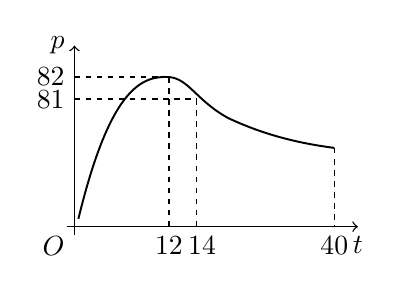
\begin{tikzpicture}[scale=1,line width=0.5pt]
\draw[->] (-0.1,0) -- (3.6,0) node[below] {$t$};
\draw[->] (0,-0.1) -- (0,2.3) node[left] {$p$};
\node[below left] at (0,0) {$O$};
\draw[line width=0.7pt] (0.05,0.1) .. controls (0.45,1.75) and (0.85,1.92) .. (1.2,1.9)
  .. controls (1.45,1.88) and (1.55,1.6) .. (1.95,1.38)
  .. controls (2.5,1.12) and (3.0,1.04) .. (3.3,1.0);
\draw[dash pattern=on 2pt off 2pt] (0,1.9) -- (1.2,1.9);
\draw[dash pattern=on 2pt off 2pt] (0,1.62) -- (1.55,1.62);
\draw[dash pattern=on 2pt off 2pt] (1.2,1.9) -- (1.2,0);
\draw[dash pattern=on 2pt off 2pt] (1.55,1.62) -- (1.55,0);
\draw[dash pattern=on 2pt off 2pt] (3.3,1.0) -- (3.3,0);
\node[left] at (0,1.9) {$82$};
\node[left] at (0,1.62) {$81$};
\node[below] at (1.2,0) {$12$};
\node[below] at (1.62,0) {$14$};
\node[below] at (3.3,0) {$40$};
\end{tikzpicture}
\end{center}

\ansspace*[12]

\ifanswer
\solbegin
\stepm{（1）}{由题意得当 $t\in(0,14]$ 时，设 $f(t)=c(t-12)^2+82$（$c<0$），}
\step{又 $f(14)=81$，所以 $c(14-12)^2+82=81$，解得 $c=-\dfrac14$；}
\step{所以 $f(t)=-\dfrac14(t-12)^2+82$,$t\in(0,14]$；}
\step{又当 $t\in[14,40]$ 时，函数 $y=\log_a(t-5)+83$（$a>0$ 且 $a\neq1$），}
\step{又当 $x=14$ 时，$y=81$，所以 $81=\log_a(14-5)+83$，解得 $a=\dfrac13$；}
\step{所以 $f(t)=\log_\frac13(t-5)+83$,$t\in[14,40]$，}
\step{所以 $p=\begin{cases}-\dfrac14(t-12)^2+82, & t\in(0,14]\\ \log_\frac13(t-5)+83, & t\in(14,40]\end{cases}$；}
\stepm{（2）}{当 $t=32$ 时，$p=\log_\frac13(32-5)+83=80$，}
\step{所以当一位学生在坚持听课 32 分钟时，注意力指数 $p$ 大约为 80；}
\stepm{（3）}{当 $t\in(0,14]$ 时，$-\dfrac14(t-12)^2+82\geqslant80$，解得 $t\in[12-2\sqrt2,14]$，}
\step{当 $t\in[14,40]$ 时，$\log_\frac13(t-5)+83\geqslant80$，解得 $5<t\leqslant32$，则 $t\in[14,32]$，}
\step{因此当 $t\in[12-2\sqrt2,32]$ 时学生听课效果最佳，}
\step{此时 $\Delta t=32-(12-2\sqrt2)=20+2\sqrt2>20$，}
\step{所以老师能经过合理安排时间在学生听课效果最佳时段讲完.}
\solend

\fi

\item 已知 $a\in R$，函数 $f(x+1)=\log_2\left(\dfrac{ax+1+a}{x+1}\right)$.

（1）若 $a=2$，求函数 $f(x)$ 的表达式及定义域；

（2）若关于 $x$ 的方程 $f\left(\dfrac x2\right)-\log_2[(a-2)x+3a-5]=0$ 的解集中恰好只有一个元素，求实
数 $a$ 的取值范围.

\ansspace*[14]

\ifanswer
\solbegin
\stepm{（1）}{$f(x+1)=\log_2\left(\dfrac{ax+1+a}{x+1}\right)$，}
\step{令 $x+1=t$，则 $f(t)=\log_2\left(\dfrac1t+a\right)$，即 $f(x)=\log_2\left(\dfrac1x+a\right)$，}
\step{因为 $a=2$，所以 $f(x)=\log_2\left(2+\dfrac1x\right)$，}
\step{由 $2+\dfrac1x>0$ 得定义域为 $\left(-\infty,-\dfrac12\right)\cup(0,+\infty)$；}
\stepm{（2）}{由（1）得 $f(x)=\log_2\left(\dfrac1x+a\right)$，}
\step{方程 $f\left(\dfrac x2\right)-\log_2[(a-2)x+3a-5]=0$，}
\step{即 $\log_2\left(\dfrac2x+a\right)-\log_2[(a-2)x+3a-5]=0$，}
\step{可转化为 $(a-2)x^2+(2a-5)x-2=0$，且 $\dfrac2x+a>0$.}
\step{①当 $a-2=0$，即 $a=2$ 时，$x=-2$，符合题意；}
\step{②当 $a-2\neq0$，即 $a\neq2$ 时，$x_1=-2$,$x_2=\dfrac1{a-2}$，}
\step{（$i$）当 $-2=\dfrac1{a-2}$ 时，即 $a=\dfrac32$ 时，符合题意；}
\step{（$ii$）当 $-2\neq\dfrac1{a-2}$ 时，即 $a\neq\dfrac32$ 且 $a\neq2$ 时，}
\step{要满足题意，则有 $\begin{cases}-1+a>0\\ 3a-4\leqslant0\end{cases}\Rightarrow1<a\leqslant\dfrac43$ 或 $\begin{cases}-1+a\leqslant0\\ 3a-4>0\end{cases}$，无解；}
\step{综上，$a$ 的取值范围 $\left(1,\dfrac43\right]\cup\left\{2,\dfrac32\right\}$.}
\solend

\fi

\item 已知函数 $y=f(x)$ 是定义在 $[0,+\infty)$ 上的函数，并且 $f(x)\geqslant0$，对于定义域内的任意自
变量的值 $x$、$y$，满足 $f(y)f(x^2f(y)+xf(y))=f(x^2+y+x)$，$f(a)=0$，其中
$a>0$.

（1）当 $f(0)\neq0$ 时，求 $f(0)$；

（2）已知当 $0\leqslant x<a$ 时，有 $f(x)\neq0$.

（$i$）求 $f(a+3)$；

（$ii$）求函数 $y=f(x)$ 的解析式（用 $a$ 表示）.

\ansspace*[16]

\ifanswer
\solbegin
\stepm{（1）}{因为 $f(x)\geqslant0$，且对于定义域内的任意自变量的值 $x$、$y$，}
\step{满足 $f(y)f(x^2f(y)+xf(y))=f(x^2+y+x)$，}
\step{令 $x=y=0$，则 $f^2(0)=f(0)$，因为 $f(0)\neq0$，所以 $f(0)=1$，}
\stepm{（2）}{（$i$）由 $f(y)f(x^2f(y)+xf(y))=f(x^2+y+x)$，}
\step{得 $f(y)f[(x^2+x)f(y)]=f[(x^2+x)+y]$，}
\step{令 $t=x^2+x$，因为 $x\geqslant0$，所以 $t=x^2+x\in[0,+\infty)$，}
\step{所以有 $f(y)f(tf(y))=f(t+y)$，因为 $f(a)=0$，}
\step{令 $y=a$，$t=3$，得 $f(a+3)=f(a)f(3f(a))=0\times f(3f(a))=0$；}
\step{（$ii$）当 $x\geqslant a$ 时，令 $y=a$，$t=x-a$，}
\step{$f(x)=f(x-a+a)=f(a)f[(x-a)f(a)]=0$.}
\step{当 $0\leqslant x<a$ 时，则有 $0<a-x\leqslant a$，令 $y=x$，$t=a-x$，}
\step{则 $f(a)=f(a-x+x)=f(x)f[(a-x)f(x)]=0$.}
\step{因为 $f(x)\neq0$，所以有 $f((a-x)f(x))=0$，则 $(a-x)f(x)\geqslant a$，}
\step{又因为 $a-x>0$，即 $f(x)\geqslant\dfrac a{a-x}$.}
\step{令 $t=\dfrac a{f(x)}>0$,$y=x>0$，}
\step{则 $f\left(\dfrac a{f(x)}+x\right)=f(x)\cdot f\left(\dfrac a{f(x)}\cdot f(x)\right)=f(x)\cdot f(a)=0$，}
\step{所以有 $\dfrac a{f(x)}+x\geqslant a$，即 $\dfrac a{f(x)}\geqslant a-x$，得 $f(x)\leqslant\dfrac a{a-x}$，}
\step{所以当 $0\leqslant x<a$ 时，$f(x)=\dfrac a{a-x}$.}
\step{综上，$f(x)=\begin{cases}\dfrac a{a-x}, & 0\leqslant x<a\\ 0, & x\geqslant a\end{cases}$.}
\solend

\fi

\end{enumerate}

\end{document}
"
% 紧凑版：xelatex "\def\iscompact{1}% 高一105_交附闵行_周末作业10.30.tex
%   —— 高一上数学“2026-2027 年交附闵行高一上周末作业 10.30”（试卷版/答案版）
% 试卷版：xelatex 高一105_交附闵行_周末作业10.30.tex
% 答案版：xelatex "\def\isanswer{1}% 高一105_交附闵行_周末作业10.30.tex
%   —— 高一上数学“2026-2027 年交附闵行高一上周末作业 10.30”（试卷版/答案版）
% 试卷版：xelatex 高一105_交附闵行_周末作业10.30.tex
% 答案版：xelatex "\def\isanswer{1}\input{高一105_交附闵行_周末作业10.30.tex}"
% 紧凑版：xelatex "\def\iscompact{1}\input{高一105_交附闵行_周末作业10.30.tex}"
%
% 原始材料：微信公众号“魔都数学加油站”文章，作者破晓，2026-11-02 17:41 发布；
% 连载“27学年高一105”，原文标题“27学年高一105——2026-2027年上海市交附闵行高一上周末作业10.30”；
% 原文链接：https://mp.weixin.qq.com/s/XUfNEvGHjD0CB5jdoleBWw。
% 正文为 13 张 PNG 页（第 4、9、13 页 2560×3620，其余 4762×6735），题目下印有【解析】，为讲评版。
% 题目、解析均据原图转录；卷面水印及公众号页脚未录入。
%
% 卷首标题：原卷印作“2026-2027 年交附闵行高一上周末作业 10.30”（公众号标题中的“上海市”
% 卷面标题行没有，本稿照卷面），年份区间按全稿惯例排 en dash；原卷未印副标题，本稿按题目
% 内容标为“函数、不等式”（主体为指数与对数，第 3 题集合、第 16 题基本不等式）。
%
% 与原卷的排版差异：
%   ① 原文从第 3 题起，填空题编号为 3—12、选择题为 13—16、解答题为 17—21，本稿保留原题号；
%   ② 原卷每题下直接印【解析】，本稿按全稿惯例将解析置于答案版；选择题括号内未印答案，另由
%      解析末句“故选 X”给出；
%   ③ 原卷未印副标题，本稿按“知识模块”口径补出；
%   ④ 原卷填空横线按全稿惯例排为 \blankline[4.4em]；解答题按惯例加 \ansspace；选择题括号排
%      \mbox{（\quad）}、选项段前按惯例加 \keepwithprev；
%   ⑤ $f(x_1)_{max}$、$g(x)_max$、$\left(\frac{a+b+c}{b-a}\right)_{min}$ 等下标原卷排斜体，
%      按 高一96 成例改正体 $\max$、$\min$；
%   ⑥ 原卷数集排斜体 $R$／$Q$，按全稿惯例改 $\R$／$\Q$；
%   ⑦ 第 11 题解析的两幅三角形示意图与第 19 题题干的 $p$-$t$ 曲线图均按原图形状用 TikZ 重排
%      （第 19 题图属题干、三版都出；第 11 题图属解析、仅答案版显示）。
%
% 原卷存疑／笔误（均照录加注）：
%   第 14 题解析“但 $16=4^x=2^y=16$”（链首、链尾的两个 $16$ 系原卷笔误，按上下文应为
%   $4^x=2^y=16$）；
%   第 16 题选项的区间分隔逗号 A 项排半角、B／C／D 三项排全角（原卷自身不一致）；
%   第 21 题 (2) 的小问号排“（$i$）求…”（右括号紧贴“求”字），照录。
%
% 行数核对：逐题数 \step/\stepm 条数，合计 159 条（Q3：2；Q4：1；Q5：4；Q6：6；Q7：3；
% Q8：7；Q9：5；Q10：3；Q11：15；Q12：7；Q13：12；Q14：7；Q15：9；Q16：10；Q17：7；
% Q18：14；Q19：14；Q20：14；Q21：19），与原卷印刷行逐题相等。
%
\documentclass[a4paper,11pt]{article}
\usepackage{common}

\begin{document}

\examtitlest[3]{2026--2027 年交附闵行高一上周末作业 10.30}{函数、不等式}

\bigsec{一、填空题}

\begin{enumerate}
\setcounter{enumi}{2}

\item 已知集合 $M=\{1,m\}$，$N=\{n,\log_2n\}$，若 $M=N$，则 $(m-n)^{2027}=$\blankline[4.4em].

\ifanswer
\solbegin
\step{由题意得 $\begin{cases}n=1\\ \log_2n=m\end{cases}$ 或 $\begin{cases}n=m\\ \log_2n=1\end{cases}$，解得 $\begin{cases}n=1\\ m=0\end{cases}$ 或 $\begin{cases}n=2\\ m=2\end{cases}$，}
\step{所以 $(m-n)^{2027}=-1$ 或 $0$.}
\solend

\fi

\item 已知 $\log_{2x^2-1}(3x^2+2x-1)=1$，则 $x=$\blankline[4.4em].

\ifanswer
\solbegin
\step{因为 $\log_{2x^2-1}(3x^2+2x-1)=1$，所以 $\begin{cases}2x^2-1>0\\ 2x^2-1\neq1\\ 3x^2+2x-1>0\\ 2x^2-1=3x^2+2x-1\end{cases}$，解得 $x=-2$.}
\solend

\fi

\item 已知 $m>1$，$n>1$，$\lg m=\log_n100$，则 $mn$ 的最小值为\blankline[4.4em].

\ifanswer
\solbegin
\step{由 $m>1$，$n>1$，得 $\lg m>0$，$\lg n>0$，}
\step{因为 $\lg m=\log_n100=\dfrac{\lg100}{\lg n}=\dfrac2{\lg n}$，所以 $\lg m\cdot\lg n=2$，}
\step{所以 $\lg(mn)=\lg m+\lg n\geqslant2\sqrt{\lg m\cdot\lg n}=2\sqrt2$，}
\step{当且仅当 $m=n=10^{\sqrt2}$ 时取等号，则 $mn\geqslant10^{2\sqrt2}$，即 $mn$ 的最小值为 $10^{2\sqrt2}$.}
\solend

\fi

\item 设 $m$、$n$ 分别是方程 $\log_{2013}x+x-9=0$ 和 $2013^x+x-9=0$ 的根，则 $m+n=$\blankline[4.4em].

\ifanswer
\solbegin
\step{由 $\log_{2013}x+x-9=0$，得 $\log_{2013}x=-x+9$，}
\step{因为 $m$ 是方程 $\log_{2013}x+x-9=0$ 的根，}
\step{所以 $m$ 为函数 $y=\log_{2013}x$ 与 $y=-x+9$ 图象交点的横坐标，}
\step{同理 $n$ 是函数 $y=2013^x$ 与 $y=-x+9$ 图象交点的横坐标，}
\step{因为 $y=\log_{2013}x$ 与 $y=2013^x$ 互为反函数，其图象关于直线 $y=x$ 对称，}
\step{联立 $\begin{cases}y=-x+9\\ y=x\end{cases}$，解得 $x=\dfrac92$，所以 $m+n=\dfrac92\times2=9$.}
\solend

\fi

\item 已知函数 $f(x)=\dfrac1{\log_2(x^2+4)}$，则 $f(-2)=$\blankline[2em]，$f(x)$ 的值域为\blankline[4.4em].

\ifanswer
\solbegin
\step{$f(-2)=\dfrac1{\log_28}=\dfrac13$.}
\step{因为 $x^2+4\geqslant4$，所以 $\log_2(x^2+4)\geqslant\log_24=2$，所以 $0<\dfrac1{\log_2(x^2+4)}\leqslant\dfrac12$，}
\step{故 $f(x)$ 的值域为 $\left(0,\dfrac12\right]$.}
\solend

\fi

\item 已知 $\alpha$、$\beta$ 是方程 $9^x-2m\cdot3^x+m^2-1=0$ 的两个根，若 $\alpha+\beta=1$，则 $\alpha\beta=$\blankline[4.4em].

\ifanswer
\solbegin
\step{由题意得方程 $9^x-2m\cdot3^x+m^2-1=0$ 有两个根，}
\step{则方程 $t^2-2mt+m^2-1=0$ 有二正根，}
\step{则 $\begin{cases}\Delta=4m^2-4(m^2-1)\geqslant0\\ 2m>0\\ m^2-1>0\end{cases}$，解得 $m>1$，}
\step{又 $\alpha$、$\beta$ 是方程 $9^x-2m\cdot3^x+m^2-1=0$ 的两个根，}
\step{则 $3^\alpha\times3^\beta=m^2-1$，又 $\alpha+\beta=1$，则 $m^2-1=3^{\alpha+\beta}=3$，}
\step{解得 $m=2$ 或 $m=-2$（舍），则 $3^\alpha+3^\beta=2m=4$，又 $\alpha=1-\beta$，}
\step{则 $3^{1-\beta}+3^\beta=4$，解得 $\beta=0$ 或 $\beta=1$，则 $\begin{cases}\alpha=1\\ \beta=0\end{cases}$ 或 $\begin{cases}\alpha=0\\ \beta=1\end{cases}$，则 $\alpha\beta=0$.}
\solend

\fi

\item 已知 $a>b>0$，$\ln a=2\ln b$，且 $a\lg b=b\lg a$，则 $a+b=$\blankline[4.4em].

\ifanswer
\solbegin
\step{因为 $a>b>0$，$\ln a=2\ln b=\ln b^2$，所以 $a=b^2$，}
\step{由 $a\lg b=b\lg a$ 得 $b^2\lg b=b\lg b^2$，即 $b\lg b=2\lg b$，所以 $b=1$ 或 $b=2$，}
\step{当 $b=2$，$a=4$，满足题意，}
\step{当 $b=1$ 时，$a=1$ 与 $a>b>0$ 矛盾，所以 $b=1$ 舍去，}
\step{所以 $a+b=6$.}
\solend

\fi

\item 函数 $f(x)=\begin{cases}2^x, & x\leqslant t\\ \log_\frac12x, & x>t\end{cases}$ 的值域为 $M$，且 $8\notin M$，则实数 $t$ 的取值集合为\blankline[4.4em].

\ifanswer
\solbegin
\step{当 $x\leqslant t$ 时，函数 $f(x)=2^x$ 在 $(-\infty,t]$ 严格增，}
\step{当 $x>t$ 时，$f(x)=\log_\frac12x$ 在 $(t,+\infty)$ 严格减，}
\step{若 $8\notin M$，则满足条件 $\begin{cases}2^t<8\\ \log_\frac12t\leqslant8\end{cases}\Rightarrow\dfrac1{256}\leqslant t<3$，故实数 $t$ 的取值集合为 $\left[\dfrac1{256},3\right)$.}
\solend

\fi

\item 德国数学家狄利克雷在数学领域成就显著，以其命名函数 $D(x)=\begin{cases}1, & x\text{为有理数}\\ 0, & x\text{为无理数}\end{cases}$，该函
数被称为狄利克雷函数。那么是否存在三个点 $A(x_1,D(x_1))$、$B(x_2,D(x_2))$、$C(x_3,D(x_3))$，
使得 $\triangle ABC$ 为等边三角形，若不存在请在横线上填写“不存在”，如果存在则在横线上填写
该正三角形的面积\blankline[4.4em].

\ifanswer
\solbegin
\step{因为 $D(x)=\begin{cases}1, & x\text{为有理数}\\ 0, & x\text{为无理数}\end{cases}$，所以 $D(x)=0$ 或 1，}
\step{设存在三个点 $A(x_1,D(x_1))$、$B(x_2,D(x_2))$、$C(x_3,D(x_3))$，}
\step{使得 $\triangle ABC$ 为等边三角形，则 $D(x_1)$、$D(x_2)$、$D(x_3)$ 不同时为 0 或 1，}
\step{不妨设 $x_1<x_2<x_3$，分析得 $\triangle ABC$ 的位置有两种情况，}
\step{第一种情况：当 $x_1$ 为有理数时，即 $D(x_1)=1$，如图，过点 $B$ 作 $BD\perp AC$，}
\begin{center}
% 原图第 4 页解析示意图按原图形状用 TikZ 重排（第一种情况：$B$ 在 $x$ 轴上、$AC$ 在上方）。
\begin{tikzpicture}[scale=1,line width=0.5pt]
\draw (0,1.2) -- (2.6,1.2);
\node at (0.25,1.4) {$A$};
\node at (1.3,1.4) {$D$};
\node at (2.35,1.4) {$C$};
\draw[dash pattern=on 2pt off 2pt] (1.3,1.2) -- (1.3,0);
\draw (1.16,1.2) -- (1.16,1.06) -- (1.3,1.06);
\draw[->] (-0.5,0) -- (3.1,0) node[below] {$x$};
\node at (1.3,-0.24) {$B$};
\end{tikzpicture}
\end{center}
\step{垂足为 $D$，得 $BD=1$，$AD=\dfrac{\sqrt3}3$，$AB=AC=BC=\dfrac{2\sqrt3}3$，}
\step{则 $x_2=x_1+AD=x_1+\dfrac{\sqrt3}3$ 为无理数，$x_3=x_1+\dfrac{2\sqrt3}3$ 为无理数，}
\step{即 $D(x_2)=0$，$D(x_3)=0$ 与图形不一致，舍去；}
\step{第二种情况：当 $x_1$ 为无理数时，即 $D(x_1)=0$，如图，}
\step{过点 $B$ 作 $BD\perp AC$，垂足为 $D$，得 $BD=1$，$AD=\dfrac{\sqrt3}3$，}
\begin{center}
% 原图第 4 页解析示意图按原图形状用 TikZ 重排（第二种情况：$B$ 在上方、$AC$ 在 $x$ 轴上）。
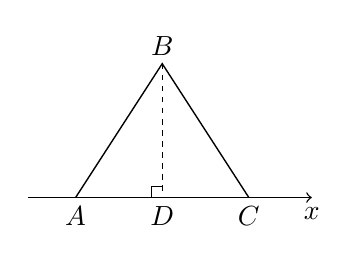
\begin{tikzpicture}[scale=1,line width=0.5pt]
\draw[->] (-0.4,0) -- (3.2,0) node[below] {$x$};
\draw (0.2,0) -- (1.3,1.7) -- (2.4,0);
\node at (0.2,-0.24) {$A$};
\node at (1.3,-0.24) {$D$};
\node at (2.4,-0.24) {$C$};
\node at (1.3,1.92) {$B$};
\draw[dash pattern=on 2pt off 2pt] (1.3,1.7) -- (1.3,0);
\draw (1.16,0) -- (1.16,0.14) -- (1.3,0.14);
\end{tikzpicture}
\end{center}
\step{$AB=AC=BC=\dfrac{2\sqrt3}3$，则 $x_2=x_1+AD=x_1+\dfrac{\sqrt3}3$，$x_3=x_1+\dfrac{2\sqrt3}3$，}
\step{存在 $x_1=-\dfrac{\sqrt3}3$，使得 $x_2=x_1+\dfrac{\sqrt3}3=0\in\Q$，且 $x_3=x_1+\dfrac{2\sqrt3}3=\dfrac{\sqrt3}3$ 为无理数，}
\step{即 $D(x_2)=1$，$D(x_3)=0$ 与图形一致，符合题意，}
\step{此时，$S_{\triangle ABC}=\dfrac12AC\cdot BD=\dfrac{\sqrt3}3$.}
\step{综上所述，存在这样的点 $A$、$B$、$C$，该正三角形的面积为 $\dfrac{\sqrt3}3$.}
\solend

\fi

\item 已知函数 $f(x)$ 满足：对 $\forall x\in R$，都有 $f(x+2025)\leqslant f(x)+2026$，
$f(x+2026)\geqslant f(x)+2027$，若 $f(1)=0$，则 $f(2)$ 的取值范围是\blankline[4.4em].

\ifanswer
\solbegin
\step{对 $\forall x\in R$，都有 $f(x+2025)\leqslant f(x)+2026$，$f(x+2026)\geqslant f(x)+2027$，}
\step{则 $f(x)+2027\leqslant f(x+2026)=f(x+1+2025)\leqslant f(x+1)+2026$，}
\step{即 $f(x)+1\leqslant f(x+1)$，所以 $f(2)\geqslant f(1)+1=1$；}
\step{$f(x)+2026\geqslant f(x+2025)=f(x+2024+1)\geqslant f(x+2024)+1$}
\step{$\geqslant\cdots\geqslant f(x+1)+2024$，所以 $f(x)+2\geqslant f(x+1)$，}
\step{所以 $f(2)\leqslant f(1)+2=2$；}
\step{即 $f(2)$ 的取值范围是 $[1,2]$.}
\solend

\fi

\end{enumerate}

\bigsec{二、选择题}

\begin{enumerate}
\setcounter{enumi}{12}

\item 若实数 $0<m<n<1$，而实数 $x>1$，则下列不等式正确的是\mbox{（\quad）}

\keepwithprev
A. $m^x<n^x$\qquad\qquad B. $x^m>x^n$\qquad\qquad C. $\log_xm>\log_xn$\qquad D. $\log_mx<\log_nx$

\ifanswer
\solbegin
\step{对于 $A$，函数 $f(t)=t^x$ 是以 $t$ 为变量，$x$ 为常量的幂函数，}
\step{由于 $x>1$，易得 $f(t)$ 在 $(0,+\infty)$ 上严格增，}
\step{$0<m<n<1$，$x>1$，可以得到 $m^x<n^x$，故 $A$ 正确；}
\step{对于 $B$，函数 $g(s)=x^s$，是以 $s$ 为变量，$x$ 为常量的指数函数，}
\step{由于 $x>1$，则 $g(s)$ 严格增，$0<m<n<1$，可以得到 $x^m<x^n$，故 $B$ 不正确；}
\step{对于 $C$，$\log_xm=\dfrac{\lg m}{\lg x}$，$\log_xn=\dfrac{\lg n}{\lg x}$，由于 $0<m<n<1$，则 $\lg m<\lg n<0$，}
\step{$x>1$，则 $\lg x>0$，则有 $\dfrac{\lg m}{\lg x}<\dfrac{\lg n}{\lg x}$，即 $\log_xm<\log_xn$，故 $C$ 不正确；}
\step{对于 $D$，由 $\log_mx-\log_nx=\dfrac{\lg x}{\lg m}-\dfrac{\lg x}{\lg n}=\dfrac{\lg x(\lg n-\lg m)}{\lg m\lg n}$，}
\step{因为实数 $0<m<n<1$，而实数 $x>1$，}
\step{所以 $\lg x>0$，$\lg m<\lg n<0$，则 $\dfrac{\lg x(\lg n-\lg m)}{\lg m\lg n}>0$，即 $\log_mx>\log_nx$，}
\step{故 $D$ 不正确.}
\step{故选 $A$.}
\solend

\fi

\item 已知 $x>1$，$y>1$，则 “$4^x>2^y$” 是 $\log_2x>\log_4(y-1)$ ”的\mbox{（\quad）}

\keepwithprev
A. 充分不必要条件\qquad\qquad B. 必要不充分条件

C. 充要条件\qquad\qquad D. 既不充分也不必要条件

\ifanswer
\solbegin
\step{因为 $x>1$，$y>1$，若 $4^x>2^y$，即 $2^{2x}>2^y$，所以 $2x>y>1$，}
\step{因为 $\dfrac y2-\sqrt{y-1}=\dfrac{(\sqrt{y-1})^2-2\sqrt{y-1}+1}2=\dfrac{(\sqrt{y-1}-1)^2}2\geqslant0$，}
\step{即 $\dfrac y2\geqslant\sqrt{y-1}>0$，所以 $\log_2\dfrac y2\geqslant\log_2\sqrt{y-1}=\dfrac12\log_2(y-1)=\log_4(y-1)$，}
\step{又 $x>\dfrac y2>\dfrac12$，所以 $\log_2x>\log_2\dfrac y2\geqslant\log_4(y-1)$，故充分性成立；}
\step{取 $x=2$，$y=4$，满足 $1=\log_2x>\log_4(y-1)=\log_43$，}
\step{但 $16=4^x=2^y=16$，即不满足 $4^x>2^y$，故必要性不成立.}% 链首链尾两个 16 系原卷笔误，应为 4^x=2^y=16，照录
\step{故选 $A$.}
\solend

\fi

\item 以下命题中，真命题的个数是\mbox{（\quad）}

①函数 $y=(x^2+1)^2+3$ 最小值为 3；②若 $2^a+\log_2a=4^b+2\log_4b$，则 $a<2b$；③不等式
$2^x-x-1>0$ 的解集为 $(1,+\infty)$.

\keepwithprev
A. $0$\qquad\qquad B. $1$\qquad\qquad C. $2$\qquad\qquad D. $3$

\ifanswer
\solbegin
\step{对于①，由于 $x^2+1\geqslant1$，则 $y=(x^2+1)^2+3\geqslant4$，}
\step{即函数 $y=(x^2+1)^2+3$ 最小值为 4，①错误；}
\step{对于②，由于 $b>0$，}
\step{则有 $2^a+\log_2a=4^b+2\log_4b=2^{2b}+\log_2b<2^{2b}+\log_22b$，}
\step{设 $f(x)=2^x+\log_2x$，易得 $f(x)$ 在 $(0,+\infty)$ 上为严格增函数，必有 $a<2b$，}
\step{②正确；}
\step{对于③，当 $x=-1$ 时，$2^x-x-1=2^x(x+1)>0$，即 $-1$ 在不等式的解集内，}
\step{③错误；}
\step{故选 $B$.}
\solend

\fi

\item 已知函数 $f(x)=ax^2+bx+c$（$a\neq0$ 且 $a<b$），若对任意的 $x\in R$，$f(x)\geqslant0$，且
$f(1)\geqslant\lambda(b-a)$，则实数 $\lambda$ 的取值范围为\mbox{（\quad）}

\keepwithprev
A. $(-\infty,2]$\qquad\qquad B. $[2\text{，}+\infty)$\qquad\qquad C. $(-\infty\text{，}3]$\qquad\qquad D. $[3\text{，}+\infty)$% 原卷 B/C/D 用全角逗号、A 用半角，照录

\ifanswer
\solbegin
\step{因为函数 $f(x)\geqslant0$ 恒成立，所以 $a>0$，且 $\Delta=b^2-4ac\leqslant0$，即 $c\geqslant\dfrac{b^2}{4a}$，}
\step{所以 $a+b+c\geqslant a+b+\dfrac{b^2}{4a}$，又 $a<b$，所以 $b-a>0$，}
\step{又 $f(1)\geqslant\lambda(b-a)$ 恒成立，所以 $a+b+c\geqslant\lambda(b-a)$ 恒成立，}
\step{即 $\lambda\leqslant\left(\dfrac{a+b+c}{b-a}\right)_{\min}=\dfrac{a+b+\dfrac{b^2}{4a}}{b-a}$，}
\step{令 $t=\dfrac ba$（$t>1$），则 $\dfrac{a+b+\dfrac{b^2}{4a}}{b-a}=\dfrac{1+t+\dfrac{t^2}4}{t-1}$，}
\step{令 $\mu=t-1$（$\mu>0$），则 $t=\mu+1$，}
\step{故上式 $=\dfrac{1+\mu+1+\dfrac{(\mu+1)^2}4}{\mu}=\dfrac14\left(\mu+\dfrac9\mu+6\right)$，}
\step{对 $\mu>0$，有 $\mu+\dfrac9\mu\geqslant2\sqrt{\mu\times\dfrac9\mu}=6$，当且仅当 $\mu=\dfrac9\mu$，即 $\mu=3$ 时取等号，}
\step{所以 $\dfrac14\left(\mu+\dfrac9\mu+6\right)\geqslant\dfrac14(6+6)=3$，故 $\lambda\leqslant3$，}
\step{即实数 $\lambda$ 的取值范围为 $(-\infty,3]$. 故选 $C$.}
\solend

\fi

\end{enumerate}

\bigsec{三、解答题}

\begin{enumerate}
\setcounter{enumi}{16}

\item 已知函数 $f(x)=\log_\frac23(ax^2-6x+18)$.

（1）若 $f(x)$ 的定义域为 $R$，求实数 $a$ 的取值范围.

（2）若 $f(x)$ 的值域为 $R$，求实数 $a$ 的取值范围.

\ansspace*[10]

\ifanswer
\solbegin
\stepm{（1）}{由 $f(x)=\log_\frac23(ax^2-6x+18)$ 的定义域为 $R$，得 $ax^2-6x+18>0$ 恒成立，}
\step{$a=0$ 时，$f(x)=\log_\frac23(18-6x)$ 的定义域为 $(-\infty,3)$，不符合题意.}
\step{$a\neq0$ 时，$\begin{cases}a>0\\ \Delta=36-4\times18a<0\end{cases}$，解得 $a>\dfrac12$.}
\step{综上，$a$ 的取值范围是 $\left(\dfrac12,+\infty\right)$.}
\stepm{（2）}{$a=0$ 时，$f(x)=\log_\frac23(18-6x)$ 的值域为 $R$，符合题意.}
\step{$a\neq0$ 时，$\begin{cases}a>0\\ \Delta=36-4\times18a\geqslant0\end{cases}$，解得 $0<a\leqslant\dfrac12$.}
\step{综上，$a$ 的取值范围是 $\left[0,\dfrac12\right]$.}
\solend

\fi

\item 已知 $f(x)=\log_ax+\log_a(6-x)$，$a>0$ 且 $a\neq1$，且 $f(3)=2$.

（1）求 $a$ 的值及 $f(x)$ 的单调区间.

（2）若对于 $\forall x_1\in(0,6)$，$\exists x_2\in[1,9]$，使得 $f(x_1)\leqslant t+\log_3x_2$ 成立，求实数 $t$ 的取值范
围.

\ansspace*[12]

\ifanswer
\solbegin
\stepm{（1）}{已知 $f(x)=\log_ax+\log_a(6-x)$，且 $f(3)=2$.}
\step{得 $\log_a3+\log_a(6-3)=2$，即 $2\log_a3=2$，}
\step{因此 $\log_a3=1$，因此 $a=3$，因此 $f(x)=\log_3x+\log_3(6-x)$，}
\step{因为 $\begin{cases}x>0\\ 6-x>0\end{cases}$，因此 $0<x<6$，故 $f(x)$ 的定义域为 $(0,6)$；}
\step{$f(x)=\log_3(6x-x^2)$，}
\step{因为函数 $y=6x-x^2$ 在 $(0,3)$ 上严格增，在 $(3,6)$ 上严格减，}
\step{又函数 $y=\log_3x$ 为严格增函数，}
\step{由复合函数的单调性得函数 $f(x)$ 在 $(0,3)$ 上严格增，在 $(3,6)$ 上严格减；}
\stepm{（2）}{令 $g(x)=t+\log_3x$，}
\step{因为 $\forall x_1\in(0,6)$，$\exists x_2\in[1,9]$，使得 $f(x_1)\leqslant t+\log_3x_2$，}
\step{即 $f(x_{1})_{\max}\leqslant g(x_{2})_{\max}$，}
\step{其中由（1）得 $f(x_{1})_{\max}=f(3)=2$.}
\step{又 $g(x)=t+\log_3x$ 在 $[1,9]$ 上严格增，因此 $g(x)_{\max}=g(9)=t+2$，}
\step{因此 $2\leqslant t+2$，因此实数 $t$ 的取值范围为 $[0,+\infty)$.}
\solend

\fi

\item 某心理学研究小组在对学生上课注意力集中情况的调查研究中，发现其注意力指数 $p$ 与
听课时间 $t$ 之间的关系满足如图所示的曲线. 当 $t\in(0,14]$ 时，曲线是二次函数图象的一部
分，当 $t\in[14,40]$ 时，曲线是函数 $y=\log_a(t-5)+83$（$a>0$ 且 $a\neq1$）图象的一部分. 根据
专家研究，当注意力指数 $p$ 大于等于 80 时听课效果最佳.

（1）试求 $p=f(t)$ 的函数关系式；

（2）当一位学生在坚持听课 32 分钟时，注意力指数 $p$ 大约为多少？

（3）一道数学难题，讲解需要 20 分钟，问老师能否经过合理安排在学生听
课效果最佳时讲完？请说明理由.

\begin{center}
% 原图第 9 页题干 p-t 曲线图按原图形状用 TikZ 重排（三版都出）。
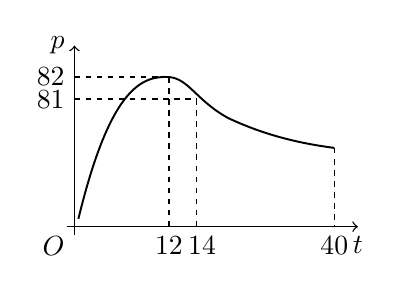
\begin{tikzpicture}[scale=1,line width=0.5pt]
\draw[->] (-0.1,0) -- (3.6,0) node[below] {$t$};
\draw[->] (0,-0.1) -- (0,2.3) node[left] {$p$};
\node[below left] at (0,0) {$O$};
\draw[line width=0.7pt] (0.05,0.1) .. controls (0.45,1.75) and (0.85,1.92) .. (1.2,1.9)
  .. controls (1.45,1.88) and (1.55,1.6) .. (1.95,1.38)
  .. controls (2.5,1.12) and (3.0,1.04) .. (3.3,1.0);
\draw[dash pattern=on 2pt off 2pt] (0,1.9) -- (1.2,1.9);
\draw[dash pattern=on 2pt off 2pt] (0,1.62) -- (1.55,1.62);
\draw[dash pattern=on 2pt off 2pt] (1.2,1.9) -- (1.2,0);
\draw[dash pattern=on 2pt off 2pt] (1.55,1.62) -- (1.55,0);
\draw[dash pattern=on 2pt off 2pt] (3.3,1.0) -- (3.3,0);
\node[left] at (0,1.9) {$82$};
\node[left] at (0,1.62) {$81$};
\node[below] at (1.2,0) {$12$};
\node[below] at (1.62,0) {$14$};
\node[below] at (3.3,0) {$40$};
\end{tikzpicture}
\end{center}

\ansspace*[12]

\ifanswer
\solbegin
\stepm{（1）}{由题意得当 $t\in(0,14]$ 时，设 $f(t)=c(t-12)^2+82$（$c<0$），}
\step{又 $f(14)=81$，所以 $c(14-12)^2+82=81$，解得 $c=-\dfrac14$；}
\step{所以 $f(t)=-\dfrac14(t-12)^2+82$,$t\in(0,14]$；}
\step{又当 $t\in[14,40]$ 时，函数 $y=\log_a(t-5)+83$（$a>0$ 且 $a\neq1$），}
\step{又当 $x=14$ 时，$y=81$，所以 $81=\log_a(14-5)+83$，解得 $a=\dfrac13$；}
\step{所以 $f(t)=\log_\frac13(t-5)+83$,$t\in[14,40]$，}
\step{所以 $p=\begin{cases}-\dfrac14(t-12)^2+82, & t\in(0,14]\\ \log_\frac13(t-5)+83, & t\in(14,40]\end{cases}$；}
\stepm{（2）}{当 $t=32$ 时，$p=\log_\frac13(32-5)+83=80$，}
\step{所以当一位学生在坚持听课 32 分钟时，注意力指数 $p$ 大约为 80；}
\stepm{（3）}{当 $t\in(0,14]$ 时，$-\dfrac14(t-12)^2+82\geqslant80$，解得 $t\in[12-2\sqrt2,14]$，}
\step{当 $t\in[14,40]$ 时，$\log_\frac13(t-5)+83\geqslant80$，解得 $5<t\leqslant32$，则 $t\in[14,32]$，}
\step{因此当 $t\in[12-2\sqrt2,32]$ 时学生听课效果最佳，}
\step{此时 $\Delta t=32-(12-2\sqrt2)=20+2\sqrt2>20$，}
\step{所以老师能经过合理安排时间在学生听课效果最佳时段讲完.}
\solend

\fi

\item 已知 $a\in R$，函数 $f(x+1)=\log_2\left(\dfrac{ax+1+a}{x+1}\right)$.

（1）若 $a=2$，求函数 $f(x)$ 的表达式及定义域；

（2）若关于 $x$ 的方程 $f\left(\dfrac x2\right)-\log_2[(a-2)x+3a-5]=0$ 的解集中恰好只有一个元素，求实
数 $a$ 的取值范围.

\ansspace*[14]

\ifanswer
\solbegin
\stepm{（1）}{$f(x+1)=\log_2\left(\dfrac{ax+1+a}{x+1}\right)$，}
\step{令 $x+1=t$，则 $f(t)=\log_2\left(\dfrac1t+a\right)$，即 $f(x)=\log_2\left(\dfrac1x+a\right)$，}
\step{因为 $a=2$，所以 $f(x)=\log_2\left(2+\dfrac1x\right)$，}
\step{由 $2+\dfrac1x>0$ 得定义域为 $\left(-\infty,-\dfrac12\right)\cup(0,+\infty)$；}
\stepm{（2）}{由（1）得 $f(x)=\log_2\left(\dfrac1x+a\right)$，}
\step{方程 $f\left(\dfrac x2\right)-\log_2[(a-2)x+3a-5]=0$，}
\step{即 $\log_2\left(\dfrac2x+a\right)-\log_2[(a-2)x+3a-5]=0$，}
\step{可转化为 $(a-2)x^2+(2a-5)x-2=0$，且 $\dfrac2x+a>0$.}
\step{①当 $a-2=0$，即 $a=2$ 时，$x=-2$，符合题意；}
\step{②当 $a-2\neq0$，即 $a\neq2$ 时，$x_1=-2$,$x_2=\dfrac1{a-2}$，}
\step{（$i$）当 $-2=\dfrac1{a-2}$ 时，即 $a=\dfrac32$ 时，符合题意；}
\step{（$ii$）当 $-2\neq\dfrac1{a-2}$ 时，即 $a\neq\dfrac32$ 且 $a\neq2$ 时，}
\step{要满足题意，则有 $\begin{cases}-1+a>0\\ 3a-4\leqslant0\end{cases}\Rightarrow1<a\leqslant\dfrac43$ 或 $\begin{cases}-1+a\leqslant0\\ 3a-4>0\end{cases}$，无解；}
\step{综上，$a$ 的取值范围 $\left(1,\dfrac43\right]\cup\left\{2,\dfrac32\right\}$.}
\solend

\fi

\item 已知函数 $y=f(x)$ 是定义在 $[0,+\infty)$ 上的函数，并且 $f(x)\geqslant0$，对于定义域内的任意自
变量的值 $x$、$y$，满足 $f(y)f(x^2f(y)+xf(y))=f(x^2+y+x)$，$f(a)=0$，其中
$a>0$.

（1）当 $f(0)\neq0$ 时，求 $f(0)$；

（2）已知当 $0\leqslant x<a$ 时，有 $f(x)\neq0$.

（$i$）求 $f(a+3)$；

（$ii$）求函数 $y=f(x)$ 的解析式（用 $a$ 表示）.

\ansspace*[16]

\ifanswer
\solbegin
\stepm{（1）}{因为 $f(x)\geqslant0$，且对于定义域内的任意自变量的值 $x$、$y$，}
\step{满足 $f(y)f(x^2f(y)+xf(y))=f(x^2+y+x)$，}
\step{令 $x=y=0$，则 $f^2(0)=f(0)$，因为 $f(0)\neq0$，所以 $f(0)=1$，}
\stepm{（2）}{（$i$）由 $f(y)f(x^2f(y)+xf(y))=f(x^2+y+x)$，}
\step{得 $f(y)f[(x^2+x)f(y)]=f[(x^2+x)+y]$，}
\step{令 $t=x^2+x$，因为 $x\geqslant0$，所以 $t=x^2+x\in[0,+\infty)$，}
\step{所以有 $f(y)f(tf(y))=f(t+y)$，因为 $f(a)=0$，}
\step{令 $y=a$，$t=3$，得 $f(a+3)=f(a)f(3f(a))=0\times f(3f(a))=0$；}
\step{（$ii$）当 $x\geqslant a$ 时，令 $y=a$，$t=x-a$，}
\step{$f(x)=f(x-a+a)=f(a)f[(x-a)f(a)]=0$.}
\step{当 $0\leqslant x<a$ 时，则有 $0<a-x\leqslant a$，令 $y=x$，$t=a-x$，}
\step{则 $f(a)=f(a-x+x)=f(x)f[(a-x)f(x)]=0$.}
\step{因为 $f(x)\neq0$，所以有 $f((a-x)f(x))=0$，则 $(a-x)f(x)\geqslant a$，}
\step{又因为 $a-x>0$，即 $f(x)\geqslant\dfrac a{a-x}$.}
\step{令 $t=\dfrac a{f(x)}>0$,$y=x>0$，}
\step{则 $f\left(\dfrac a{f(x)}+x\right)=f(x)\cdot f\left(\dfrac a{f(x)}\cdot f(x)\right)=f(x)\cdot f(a)=0$，}
\step{所以有 $\dfrac a{f(x)}+x\geqslant a$，即 $\dfrac a{f(x)}\geqslant a-x$，得 $f(x)\leqslant\dfrac a{a-x}$，}
\step{所以当 $0\leqslant x<a$ 时，$f(x)=\dfrac a{a-x}$.}
\step{综上，$f(x)=\begin{cases}\dfrac a{a-x}, & 0\leqslant x<a\\ 0, & x\geqslant a\end{cases}$.}
\solend

\fi

\end{enumerate}

\end{document}
"
% 紧凑版：xelatex "\def\iscompact{1}% 高一105_交附闵行_周末作业10.30.tex
%   —— 高一上数学“2026-2027 年交附闵行高一上周末作业 10.30”（试卷版/答案版）
% 试卷版：xelatex 高一105_交附闵行_周末作业10.30.tex
% 答案版：xelatex "\def\isanswer{1}\input{高一105_交附闵行_周末作业10.30.tex}"
% 紧凑版：xelatex "\def\iscompact{1}\input{高一105_交附闵行_周末作业10.30.tex}"
%
% 原始材料：微信公众号“魔都数学加油站”文章，作者破晓，2026-11-02 17:41 发布；
% 连载“27学年高一105”，原文标题“27学年高一105——2026-2027年上海市交附闵行高一上周末作业10.30”；
% 原文链接：https://mp.weixin.qq.com/s/XUfNEvGHjD0CB5jdoleBWw。
% 正文为 13 张 PNG 页（第 4、9、13 页 2560×3620，其余 4762×6735），题目下印有【解析】，为讲评版。
% 题目、解析均据原图转录；卷面水印及公众号页脚未录入。
%
% 卷首标题：原卷印作“2026-2027 年交附闵行高一上周末作业 10.30”（公众号标题中的“上海市”
% 卷面标题行没有，本稿照卷面），年份区间按全稿惯例排 en dash；原卷未印副标题，本稿按题目
% 内容标为“函数、不等式”（主体为指数与对数，第 3 题集合、第 16 题基本不等式）。
%
% 与原卷的排版差异：
%   ① 原文从第 3 题起，填空题编号为 3—12、选择题为 13—16、解答题为 17—21，本稿保留原题号；
%   ② 原卷每题下直接印【解析】，本稿按全稿惯例将解析置于答案版；选择题括号内未印答案，另由
%      解析末句“故选 X”给出；
%   ③ 原卷未印副标题，本稿按“知识模块”口径补出；
%   ④ 原卷填空横线按全稿惯例排为 \blankline[4.4em]；解答题按惯例加 \ansspace；选择题括号排
%      \mbox{（\quad）}、选项段前按惯例加 \keepwithprev；
%   ⑤ $f(x_1)_{max}$、$g(x)_max$、$\left(\frac{a+b+c}{b-a}\right)_{min}$ 等下标原卷排斜体，
%      按 高一96 成例改正体 $\max$、$\min$；
%   ⑥ 原卷数集排斜体 $R$／$Q$，按全稿惯例改 $\R$／$\Q$；
%   ⑦ 第 11 题解析的两幅三角形示意图与第 19 题题干的 $p$-$t$ 曲线图均按原图形状用 TikZ 重排
%      （第 19 题图属题干、三版都出；第 11 题图属解析、仅答案版显示）。
%
% 原卷存疑／笔误（均照录加注）：
%   第 14 题解析“但 $16=4^x=2^y=16$”（链首、链尾的两个 $16$ 系原卷笔误，按上下文应为
%   $4^x=2^y=16$）；
%   第 16 题选项的区间分隔逗号 A 项排半角、B／C／D 三项排全角（原卷自身不一致）；
%   第 21 题 (2) 的小问号排“（$i$）求…”（右括号紧贴“求”字），照录。
%
% 行数核对：逐题数 \step/\stepm 条数，合计 159 条（Q3：2；Q4：1；Q5：4；Q6：6；Q7：3；
% Q8：7；Q9：5；Q10：3；Q11：15；Q12：7；Q13：12；Q14：7；Q15：9；Q16：10；Q17：7；
% Q18：14；Q19：14；Q20：14；Q21：19），与原卷印刷行逐题相等。
%
\documentclass[a4paper,11pt]{article}
\usepackage{common}

\begin{document}

\examtitlest[3]{2026--2027 年交附闵行高一上周末作业 10.30}{函数、不等式}

\bigsec{一、填空题}

\begin{enumerate}
\setcounter{enumi}{2}

\item 已知集合 $M=\{1,m\}$，$N=\{n,\log_2n\}$，若 $M=N$，则 $(m-n)^{2027}=$\blankline[4.4em].

\ifanswer
\solbegin
\step{由题意得 $\begin{cases}n=1\\ \log_2n=m\end{cases}$ 或 $\begin{cases}n=m\\ \log_2n=1\end{cases}$，解得 $\begin{cases}n=1\\ m=0\end{cases}$ 或 $\begin{cases}n=2\\ m=2\end{cases}$，}
\step{所以 $(m-n)^{2027}=-1$ 或 $0$.}
\solend

\fi

\item 已知 $\log_{2x^2-1}(3x^2+2x-1)=1$，则 $x=$\blankline[4.4em].

\ifanswer
\solbegin
\step{因为 $\log_{2x^2-1}(3x^2+2x-1)=1$，所以 $\begin{cases}2x^2-1>0\\ 2x^2-1\neq1\\ 3x^2+2x-1>0\\ 2x^2-1=3x^2+2x-1\end{cases}$，解得 $x=-2$.}
\solend

\fi

\item 已知 $m>1$，$n>1$，$\lg m=\log_n100$，则 $mn$ 的最小值为\blankline[4.4em].

\ifanswer
\solbegin
\step{由 $m>1$，$n>1$，得 $\lg m>0$，$\lg n>0$，}
\step{因为 $\lg m=\log_n100=\dfrac{\lg100}{\lg n}=\dfrac2{\lg n}$，所以 $\lg m\cdot\lg n=2$，}
\step{所以 $\lg(mn)=\lg m+\lg n\geqslant2\sqrt{\lg m\cdot\lg n}=2\sqrt2$，}
\step{当且仅当 $m=n=10^{\sqrt2}$ 时取等号，则 $mn\geqslant10^{2\sqrt2}$，即 $mn$ 的最小值为 $10^{2\sqrt2}$.}
\solend

\fi

\item 设 $m$、$n$ 分别是方程 $\log_{2013}x+x-9=0$ 和 $2013^x+x-9=0$ 的根，则 $m+n=$\blankline[4.4em].

\ifanswer
\solbegin
\step{由 $\log_{2013}x+x-9=0$，得 $\log_{2013}x=-x+9$，}
\step{因为 $m$ 是方程 $\log_{2013}x+x-9=0$ 的根，}
\step{所以 $m$ 为函数 $y=\log_{2013}x$ 与 $y=-x+9$ 图象交点的横坐标，}
\step{同理 $n$ 是函数 $y=2013^x$ 与 $y=-x+9$ 图象交点的横坐标，}
\step{因为 $y=\log_{2013}x$ 与 $y=2013^x$ 互为反函数，其图象关于直线 $y=x$ 对称，}
\step{联立 $\begin{cases}y=-x+9\\ y=x\end{cases}$，解得 $x=\dfrac92$，所以 $m+n=\dfrac92\times2=9$.}
\solend

\fi

\item 已知函数 $f(x)=\dfrac1{\log_2(x^2+4)}$，则 $f(-2)=$\blankline[2em]，$f(x)$ 的值域为\blankline[4.4em].

\ifanswer
\solbegin
\step{$f(-2)=\dfrac1{\log_28}=\dfrac13$.}
\step{因为 $x^2+4\geqslant4$，所以 $\log_2(x^2+4)\geqslant\log_24=2$，所以 $0<\dfrac1{\log_2(x^2+4)}\leqslant\dfrac12$，}
\step{故 $f(x)$ 的值域为 $\left(0,\dfrac12\right]$.}
\solend

\fi

\item 已知 $\alpha$、$\beta$ 是方程 $9^x-2m\cdot3^x+m^2-1=0$ 的两个根，若 $\alpha+\beta=1$，则 $\alpha\beta=$\blankline[4.4em].

\ifanswer
\solbegin
\step{由题意得方程 $9^x-2m\cdot3^x+m^2-1=0$ 有两个根，}
\step{则方程 $t^2-2mt+m^2-1=0$ 有二正根，}
\step{则 $\begin{cases}\Delta=4m^2-4(m^2-1)\geqslant0\\ 2m>0\\ m^2-1>0\end{cases}$，解得 $m>1$，}
\step{又 $\alpha$、$\beta$ 是方程 $9^x-2m\cdot3^x+m^2-1=0$ 的两个根，}
\step{则 $3^\alpha\times3^\beta=m^2-1$，又 $\alpha+\beta=1$，则 $m^2-1=3^{\alpha+\beta}=3$，}
\step{解得 $m=2$ 或 $m=-2$（舍），则 $3^\alpha+3^\beta=2m=4$，又 $\alpha=1-\beta$，}
\step{则 $3^{1-\beta}+3^\beta=4$，解得 $\beta=0$ 或 $\beta=1$，则 $\begin{cases}\alpha=1\\ \beta=0\end{cases}$ 或 $\begin{cases}\alpha=0\\ \beta=1\end{cases}$，则 $\alpha\beta=0$.}
\solend

\fi

\item 已知 $a>b>0$，$\ln a=2\ln b$，且 $a\lg b=b\lg a$，则 $a+b=$\blankline[4.4em].

\ifanswer
\solbegin
\step{因为 $a>b>0$，$\ln a=2\ln b=\ln b^2$，所以 $a=b^2$，}
\step{由 $a\lg b=b\lg a$ 得 $b^2\lg b=b\lg b^2$，即 $b\lg b=2\lg b$，所以 $b=1$ 或 $b=2$，}
\step{当 $b=2$，$a=4$，满足题意，}
\step{当 $b=1$ 时，$a=1$ 与 $a>b>0$ 矛盾，所以 $b=1$ 舍去，}
\step{所以 $a+b=6$.}
\solend

\fi

\item 函数 $f(x)=\begin{cases}2^x, & x\leqslant t\\ \log_\frac12x, & x>t\end{cases}$ 的值域为 $M$，且 $8\notin M$，则实数 $t$ 的取值集合为\blankline[4.4em].

\ifanswer
\solbegin
\step{当 $x\leqslant t$ 时，函数 $f(x)=2^x$ 在 $(-\infty,t]$ 严格增，}
\step{当 $x>t$ 时，$f(x)=\log_\frac12x$ 在 $(t,+\infty)$ 严格减，}
\step{若 $8\notin M$，则满足条件 $\begin{cases}2^t<8\\ \log_\frac12t\leqslant8\end{cases}\Rightarrow\dfrac1{256}\leqslant t<3$，故实数 $t$ 的取值集合为 $\left[\dfrac1{256},3\right)$.}
\solend

\fi

\item 德国数学家狄利克雷在数学领域成就显著，以其命名函数 $D(x)=\begin{cases}1, & x\text{为有理数}\\ 0, & x\text{为无理数}\end{cases}$，该函
数被称为狄利克雷函数。那么是否存在三个点 $A(x_1,D(x_1))$、$B(x_2,D(x_2))$、$C(x_3,D(x_3))$，
使得 $\triangle ABC$ 为等边三角形，若不存在请在横线上填写“不存在”，如果存在则在横线上填写
该正三角形的面积\blankline[4.4em].

\ifanswer
\solbegin
\step{因为 $D(x)=\begin{cases}1, & x\text{为有理数}\\ 0, & x\text{为无理数}\end{cases}$，所以 $D(x)=0$ 或 1，}
\step{设存在三个点 $A(x_1,D(x_1))$、$B(x_2,D(x_2))$、$C(x_3,D(x_3))$，}
\step{使得 $\triangle ABC$ 为等边三角形，则 $D(x_1)$、$D(x_2)$、$D(x_3)$ 不同时为 0 或 1，}
\step{不妨设 $x_1<x_2<x_3$，分析得 $\triangle ABC$ 的位置有两种情况，}
\step{第一种情况：当 $x_1$ 为有理数时，即 $D(x_1)=1$，如图，过点 $B$ 作 $BD\perp AC$，}
\begin{center}
% 原图第 4 页解析示意图按原图形状用 TikZ 重排（第一种情况：$B$ 在 $x$ 轴上、$AC$ 在上方）。
\begin{tikzpicture}[scale=1,line width=0.5pt]
\draw (0,1.2) -- (2.6,1.2);
\node at (0.25,1.4) {$A$};
\node at (1.3,1.4) {$D$};
\node at (2.35,1.4) {$C$};
\draw[dash pattern=on 2pt off 2pt] (1.3,1.2) -- (1.3,0);
\draw (1.16,1.2) -- (1.16,1.06) -- (1.3,1.06);
\draw[->] (-0.5,0) -- (3.1,0) node[below] {$x$};
\node at (1.3,-0.24) {$B$};
\end{tikzpicture}
\end{center}
\step{垂足为 $D$，得 $BD=1$，$AD=\dfrac{\sqrt3}3$，$AB=AC=BC=\dfrac{2\sqrt3}3$，}
\step{则 $x_2=x_1+AD=x_1+\dfrac{\sqrt3}3$ 为无理数，$x_3=x_1+\dfrac{2\sqrt3}3$ 为无理数，}
\step{即 $D(x_2)=0$，$D(x_3)=0$ 与图形不一致，舍去；}
\step{第二种情况：当 $x_1$ 为无理数时，即 $D(x_1)=0$，如图，}
\step{过点 $B$ 作 $BD\perp AC$，垂足为 $D$，得 $BD=1$，$AD=\dfrac{\sqrt3}3$，}
\begin{center}
% 原图第 4 页解析示意图按原图形状用 TikZ 重排（第二种情况：$B$ 在上方、$AC$ 在 $x$ 轴上）。
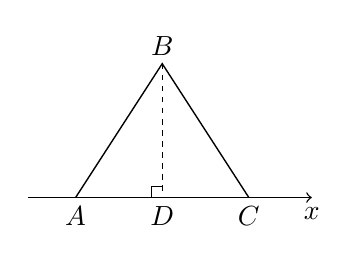
\begin{tikzpicture}[scale=1,line width=0.5pt]
\draw[->] (-0.4,0) -- (3.2,0) node[below] {$x$};
\draw (0.2,0) -- (1.3,1.7) -- (2.4,0);
\node at (0.2,-0.24) {$A$};
\node at (1.3,-0.24) {$D$};
\node at (2.4,-0.24) {$C$};
\node at (1.3,1.92) {$B$};
\draw[dash pattern=on 2pt off 2pt] (1.3,1.7) -- (1.3,0);
\draw (1.16,0) -- (1.16,0.14) -- (1.3,0.14);
\end{tikzpicture}
\end{center}
\step{$AB=AC=BC=\dfrac{2\sqrt3}3$，则 $x_2=x_1+AD=x_1+\dfrac{\sqrt3}3$，$x_3=x_1+\dfrac{2\sqrt3}3$，}
\step{存在 $x_1=-\dfrac{\sqrt3}3$，使得 $x_2=x_1+\dfrac{\sqrt3}3=0\in\Q$，且 $x_3=x_1+\dfrac{2\sqrt3}3=\dfrac{\sqrt3}3$ 为无理数，}
\step{即 $D(x_2)=1$，$D(x_3)=0$ 与图形一致，符合题意，}
\step{此时，$S_{\triangle ABC}=\dfrac12AC\cdot BD=\dfrac{\sqrt3}3$.}
\step{综上所述，存在这样的点 $A$、$B$、$C$，该正三角形的面积为 $\dfrac{\sqrt3}3$.}
\solend

\fi

\item 已知函数 $f(x)$ 满足：对 $\forall x\in R$，都有 $f(x+2025)\leqslant f(x)+2026$，
$f(x+2026)\geqslant f(x)+2027$，若 $f(1)=0$，则 $f(2)$ 的取值范围是\blankline[4.4em].

\ifanswer
\solbegin
\step{对 $\forall x\in R$，都有 $f(x+2025)\leqslant f(x)+2026$，$f(x+2026)\geqslant f(x)+2027$，}
\step{则 $f(x)+2027\leqslant f(x+2026)=f(x+1+2025)\leqslant f(x+1)+2026$，}
\step{即 $f(x)+1\leqslant f(x+1)$，所以 $f(2)\geqslant f(1)+1=1$；}
\step{$f(x)+2026\geqslant f(x+2025)=f(x+2024+1)\geqslant f(x+2024)+1$}
\step{$\geqslant\cdots\geqslant f(x+1)+2024$，所以 $f(x)+2\geqslant f(x+1)$，}
\step{所以 $f(2)\leqslant f(1)+2=2$；}
\step{即 $f(2)$ 的取值范围是 $[1,2]$.}
\solend

\fi

\end{enumerate}

\bigsec{二、选择题}

\begin{enumerate}
\setcounter{enumi}{12}

\item 若实数 $0<m<n<1$，而实数 $x>1$，则下列不等式正确的是\mbox{（\quad）}

\keepwithprev
A. $m^x<n^x$\qquad\qquad B. $x^m>x^n$\qquad\qquad C. $\log_xm>\log_xn$\qquad D. $\log_mx<\log_nx$

\ifanswer
\solbegin
\step{对于 $A$，函数 $f(t)=t^x$ 是以 $t$ 为变量，$x$ 为常量的幂函数，}
\step{由于 $x>1$，易得 $f(t)$ 在 $(0,+\infty)$ 上严格增，}
\step{$0<m<n<1$，$x>1$，可以得到 $m^x<n^x$，故 $A$ 正确；}
\step{对于 $B$，函数 $g(s)=x^s$，是以 $s$ 为变量，$x$ 为常量的指数函数，}
\step{由于 $x>1$，则 $g(s)$ 严格增，$0<m<n<1$，可以得到 $x^m<x^n$，故 $B$ 不正确；}
\step{对于 $C$，$\log_xm=\dfrac{\lg m}{\lg x}$，$\log_xn=\dfrac{\lg n}{\lg x}$，由于 $0<m<n<1$，则 $\lg m<\lg n<0$，}
\step{$x>1$，则 $\lg x>0$，则有 $\dfrac{\lg m}{\lg x}<\dfrac{\lg n}{\lg x}$，即 $\log_xm<\log_xn$，故 $C$ 不正确；}
\step{对于 $D$，由 $\log_mx-\log_nx=\dfrac{\lg x}{\lg m}-\dfrac{\lg x}{\lg n}=\dfrac{\lg x(\lg n-\lg m)}{\lg m\lg n}$，}
\step{因为实数 $0<m<n<1$，而实数 $x>1$，}
\step{所以 $\lg x>0$，$\lg m<\lg n<0$，则 $\dfrac{\lg x(\lg n-\lg m)}{\lg m\lg n}>0$，即 $\log_mx>\log_nx$，}
\step{故 $D$ 不正确.}
\step{故选 $A$.}
\solend

\fi

\item 已知 $x>1$，$y>1$，则 “$4^x>2^y$” 是 $\log_2x>\log_4(y-1)$ ”的\mbox{（\quad）}

\keepwithprev
A. 充分不必要条件\qquad\qquad B. 必要不充分条件

C. 充要条件\qquad\qquad D. 既不充分也不必要条件

\ifanswer
\solbegin
\step{因为 $x>1$，$y>1$，若 $4^x>2^y$，即 $2^{2x}>2^y$，所以 $2x>y>1$，}
\step{因为 $\dfrac y2-\sqrt{y-1}=\dfrac{(\sqrt{y-1})^2-2\sqrt{y-1}+1}2=\dfrac{(\sqrt{y-1}-1)^2}2\geqslant0$，}
\step{即 $\dfrac y2\geqslant\sqrt{y-1}>0$，所以 $\log_2\dfrac y2\geqslant\log_2\sqrt{y-1}=\dfrac12\log_2(y-1)=\log_4(y-1)$，}
\step{又 $x>\dfrac y2>\dfrac12$，所以 $\log_2x>\log_2\dfrac y2\geqslant\log_4(y-1)$，故充分性成立；}
\step{取 $x=2$，$y=4$，满足 $1=\log_2x>\log_4(y-1)=\log_43$，}
\step{但 $16=4^x=2^y=16$，即不满足 $4^x>2^y$，故必要性不成立.}% 链首链尾两个 16 系原卷笔误，应为 4^x=2^y=16，照录
\step{故选 $A$.}
\solend

\fi

\item 以下命题中，真命题的个数是\mbox{（\quad）}

①函数 $y=(x^2+1)^2+3$ 最小值为 3；②若 $2^a+\log_2a=4^b+2\log_4b$，则 $a<2b$；③不等式
$2^x-x-1>0$ 的解集为 $(1,+\infty)$.

\keepwithprev
A. $0$\qquad\qquad B. $1$\qquad\qquad C. $2$\qquad\qquad D. $3$

\ifanswer
\solbegin
\step{对于①，由于 $x^2+1\geqslant1$，则 $y=(x^2+1)^2+3\geqslant4$，}
\step{即函数 $y=(x^2+1)^2+3$ 最小值为 4，①错误；}
\step{对于②，由于 $b>0$，}
\step{则有 $2^a+\log_2a=4^b+2\log_4b=2^{2b}+\log_2b<2^{2b}+\log_22b$，}
\step{设 $f(x)=2^x+\log_2x$，易得 $f(x)$ 在 $(0,+\infty)$ 上为严格增函数，必有 $a<2b$，}
\step{②正确；}
\step{对于③，当 $x=-1$ 时，$2^x-x-1=2^x(x+1)>0$，即 $-1$ 在不等式的解集内，}
\step{③错误；}
\step{故选 $B$.}
\solend

\fi

\item 已知函数 $f(x)=ax^2+bx+c$（$a\neq0$ 且 $a<b$），若对任意的 $x\in R$，$f(x)\geqslant0$，且
$f(1)\geqslant\lambda(b-a)$，则实数 $\lambda$ 的取值范围为\mbox{（\quad）}

\keepwithprev
A. $(-\infty,2]$\qquad\qquad B. $[2\text{，}+\infty)$\qquad\qquad C. $(-\infty\text{，}3]$\qquad\qquad D. $[3\text{，}+\infty)$% 原卷 B/C/D 用全角逗号、A 用半角，照录

\ifanswer
\solbegin
\step{因为函数 $f(x)\geqslant0$ 恒成立，所以 $a>0$，且 $\Delta=b^2-4ac\leqslant0$，即 $c\geqslant\dfrac{b^2}{4a}$，}
\step{所以 $a+b+c\geqslant a+b+\dfrac{b^2}{4a}$，又 $a<b$，所以 $b-a>0$，}
\step{又 $f(1)\geqslant\lambda(b-a)$ 恒成立，所以 $a+b+c\geqslant\lambda(b-a)$ 恒成立，}
\step{即 $\lambda\leqslant\left(\dfrac{a+b+c}{b-a}\right)_{\min}=\dfrac{a+b+\dfrac{b^2}{4a}}{b-a}$，}
\step{令 $t=\dfrac ba$（$t>1$），则 $\dfrac{a+b+\dfrac{b^2}{4a}}{b-a}=\dfrac{1+t+\dfrac{t^2}4}{t-1}$，}
\step{令 $\mu=t-1$（$\mu>0$），则 $t=\mu+1$，}
\step{故上式 $=\dfrac{1+\mu+1+\dfrac{(\mu+1)^2}4}{\mu}=\dfrac14\left(\mu+\dfrac9\mu+6\right)$，}
\step{对 $\mu>0$，有 $\mu+\dfrac9\mu\geqslant2\sqrt{\mu\times\dfrac9\mu}=6$，当且仅当 $\mu=\dfrac9\mu$，即 $\mu=3$ 时取等号，}
\step{所以 $\dfrac14\left(\mu+\dfrac9\mu+6\right)\geqslant\dfrac14(6+6)=3$，故 $\lambda\leqslant3$，}
\step{即实数 $\lambda$ 的取值范围为 $(-\infty,3]$. 故选 $C$.}
\solend

\fi

\end{enumerate}

\bigsec{三、解答题}

\begin{enumerate}
\setcounter{enumi}{16}

\item 已知函数 $f(x)=\log_\frac23(ax^2-6x+18)$.

（1）若 $f(x)$ 的定义域为 $R$，求实数 $a$ 的取值范围.

（2）若 $f(x)$ 的值域为 $R$，求实数 $a$ 的取值范围.

\ansspace*[10]

\ifanswer
\solbegin
\stepm{（1）}{由 $f(x)=\log_\frac23(ax^2-6x+18)$ 的定义域为 $R$，得 $ax^2-6x+18>0$ 恒成立，}
\step{$a=0$ 时，$f(x)=\log_\frac23(18-6x)$ 的定义域为 $(-\infty,3)$，不符合题意.}
\step{$a\neq0$ 时，$\begin{cases}a>0\\ \Delta=36-4\times18a<0\end{cases}$，解得 $a>\dfrac12$.}
\step{综上，$a$ 的取值范围是 $\left(\dfrac12,+\infty\right)$.}
\stepm{（2）}{$a=0$ 时，$f(x)=\log_\frac23(18-6x)$ 的值域为 $R$，符合题意.}
\step{$a\neq0$ 时，$\begin{cases}a>0\\ \Delta=36-4\times18a\geqslant0\end{cases}$，解得 $0<a\leqslant\dfrac12$.}
\step{综上，$a$ 的取值范围是 $\left[0,\dfrac12\right]$.}
\solend

\fi

\item 已知 $f(x)=\log_ax+\log_a(6-x)$，$a>0$ 且 $a\neq1$，且 $f(3)=2$.

（1）求 $a$ 的值及 $f(x)$ 的单调区间.

（2）若对于 $\forall x_1\in(0,6)$，$\exists x_2\in[1,9]$，使得 $f(x_1)\leqslant t+\log_3x_2$ 成立，求实数 $t$ 的取值范
围.

\ansspace*[12]

\ifanswer
\solbegin
\stepm{（1）}{已知 $f(x)=\log_ax+\log_a(6-x)$，且 $f(3)=2$.}
\step{得 $\log_a3+\log_a(6-3)=2$，即 $2\log_a3=2$，}
\step{因此 $\log_a3=1$，因此 $a=3$，因此 $f(x)=\log_3x+\log_3(6-x)$，}
\step{因为 $\begin{cases}x>0\\ 6-x>0\end{cases}$，因此 $0<x<6$，故 $f(x)$ 的定义域为 $(0,6)$；}
\step{$f(x)=\log_3(6x-x^2)$，}
\step{因为函数 $y=6x-x^2$ 在 $(0,3)$ 上严格增，在 $(3,6)$ 上严格减，}
\step{又函数 $y=\log_3x$ 为严格增函数，}
\step{由复合函数的单调性得函数 $f(x)$ 在 $(0,3)$ 上严格增，在 $(3,6)$ 上严格减；}
\stepm{（2）}{令 $g(x)=t+\log_3x$，}
\step{因为 $\forall x_1\in(0,6)$，$\exists x_2\in[1,9]$，使得 $f(x_1)\leqslant t+\log_3x_2$，}
\step{即 $f(x_{1})_{\max}\leqslant g(x_{2})_{\max}$，}
\step{其中由（1）得 $f(x_{1})_{\max}=f(3)=2$.}
\step{又 $g(x)=t+\log_3x$ 在 $[1,9]$ 上严格增，因此 $g(x)_{\max}=g(9)=t+2$，}
\step{因此 $2\leqslant t+2$，因此实数 $t$ 的取值范围为 $[0,+\infty)$.}
\solend

\fi

\item 某心理学研究小组在对学生上课注意力集中情况的调查研究中，发现其注意力指数 $p$ 与
听课时间 $t$ 之间的关系满足如图所示的曲线. 当 $t\in(0,14]$ 时，曲线是二次函数图象的一部
分，当 $t\in[14,40]$ 时，曲线是函数 $y=\log_a(t-5)+83$（$a>0$ 且 $a\neq1$）图象的一部分. 根据
专家研究，当注意力指数 $p$ 大于等于 80 时听课效果最佳.

（1）试求 $p=f(t)$ 的函数关系式；

（2）当一位学生在坚持听课 32 分钟时，注意力指数 $p$ 大约为多少？

（3）一道数学难题，讲解需要 20 分钟，问老师能否经过合理安排在学生听
课效果最佳时讲完？请说明理由.

\begin{center}
% 原图第 9 页题干 p-t 曲线图按原图形状用 TikZ 重排（三版都出）。
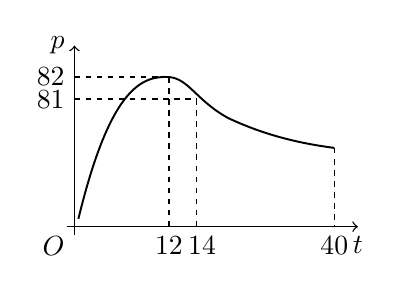
\begin{tikzpicture}[scale=1,line width=0.5pt]
\draw[->] (-0.1,0) -- (3.6,0) node[below] {$t$};
\draw[->] (0,-0.1) -- (0,2.3) node[left] {$p$};
\node[below left] at (0,0) {$O$};
\draw[line width=0.7pt] (0.05,0.1) .. controls (0.45,1.75) and (0.85,1.92) .. (1.2,1.9)
  .. controls (1.45,1.88) and (1.55,1.6) .. (1.95,1.38)
  .. controls (2.5,1.12) and (3.0,1.04) .. (3.3,1.0);
\draw[dash pattern=on 2pt off 2pt] (0,1.9) -- (1.2,1.9);
\draw[dash pattern=on 2pt off 2pt] (0,1.62) -- (1.55,1.62);
\draw[dash pattern=on 2pt off 2pt] (1.2,1.9) -- (1.2,0);
\draw[dash pattern=on 2pt off 2pt] (1.55,1.62) -- (1.55,0);
\draw[dash pattern=on 2pt off 2pt] (3.3,1.0) -- (3.3,0);
\node[left] at (0,1.9) {$82$};
\node[left] at (0,1.62) {$81$};
\node[below] at (1.2,0) {$12$};
\node[below] at (1.62,0) {$14$};
\node[below] at (3.3,0) {$40$};
\end{tikzpicture}
\end{center}

\ansspace*[12]

\ifanswer
\solbegin
\stepm{（1）}{由题意得当 $t\in(0,14]$ 时，设 $f(t)=c(t-12)^2+82$（$c<0$），}
\step{又 $f(14)=81$，所以 $c(14-12)^2+82=81$，解得 $c=-\dfrac14$；}
\step{所以 $f(t)=-\dfrac14(t-12)^2+82$,$t\in(0,14]$；}
\step{又当 $t\in[14,40]$ 时，函数 $y=\log_a(t-5)+83$（$a>0$ 且 $a\neq1$），}
\step{又当 $x=14$ 时，$y=81$，所以 $81=\log_a(14-5)+83$，解得 $a=\dfrac13$；}
\step{所以 $f(t)=\log_\frac13(t-5)+83$,$t\in[14,40]$，}
\step{所以 $p=\begin{cases}-\dfrac14(t-12)^2+82, & t\in(0,14]\\ \log_\frac13(t-5)+83, & t\in(14,40]\end{cases}$；}
\stepm{（2）}{当 $t=32$ 时，$p=\log_\frac13(32-5)+83=80$，}
\step{所以当一位学生在坚持听课 32 分钟时，注意力指数 $p$ 大约为 80；}
\stepm{（3）}{当 $t\in(0,14]$ 时，$-\dfrac14(t-12)^2+82\geqslant80$，解得 $t\in[12-2\sqrt2,14]$，}
\step{当 $t\in[14,40]$ 时，$\log_\frac13(t-5)+83\geqslant80$，解得 $5<t\leqslant32$，则 $t\in[14,32]$，}
\step{因此当 $t\in[12-2\sqrt2,32]$ 时学生听课效果最佳，}
\step{此时 $\Delta t=32-(12-2\sqrt2)=20+2\sqrt2>20$，}
\step{所以老师能经过合理安排时间在学生听课效果最佳时段讲完.}
\solend

\fi

\item 已知 $a\in R$，函数 $f(x+1)=\log_2\left(\dfrac{ax+1+a}{x+1}\right)$.

（1）若 $a=2$，求函数 $f(x)$ 的表达式及定义域；

（2）若关于 $x$ 的方程 $f\left(\dfrac x2\right)-\log_2[(a-2)x+3a-5]=0$ 的解集中恰好只有一个元素，求实
数 $a$ 的取值范围.

\ansspace*[14]

\ifanswer
\solbegin
\stepm{（1）}{$f(x+1)=\log_2\left(\dfrac{ax+1+a}{x+1}\right)$，}
\step{令 $x+1=t$，则 $f(t)=\log_2\left(\dfrac1t+a\right)$，即 $f(x)=\log_2\left(\dfrac1x+a\right)$，}
\step{因为 $a=2$，所以 $f(x)=\log_2\left(2+\dfrac1x\right)$，}
\step{由 $2+\dfrac1x>0$ 得定义域为 $\left(-\infty,-\dfrac12\right)\cup(0,+\infty)$；}
\stepm{（2）}{由（1）得 $f(x)=\log_2\left(\dfrac1x+a\right)$，}
\step{方程 $f\left(\dfrac x2\right)-\log_2[(a-2)x+3a-5]=0$，}
\step{即 $\log_2\left(\dfrac2x+a\right)-\log_2[(a-2)x+3a-5]=0$，}
\step{可转化为 $(a-2)x^2+(2a-5)x-2=0$，且 $\dfrac2x+a>0$.}
\step{①当 $a-2=0$，即 $a=2$ 时，$x=-2$，符合题意；}
\step{②当 $a-2\neq0$，即 $a\neq2$ 时，$x_1=-2$,$x_2=\dfrac1{a-2}$，}
\step{（$i$）当 $-2=\dfrac1{a-2}$ 时，即 $a=\dfrac32$ 时，符合题意；}
\step{（$ii$）当 $-2\neq\dfrac1{a-2}$ 时，即 $a\neq\dfrac32$ 且 $a\neq2$ 时，}
\step{要满足题意，则有 $\begin{cases}-1+a>0\\ 3a-4\leqslant0\end{cases}\Rightarrow1<a\leqslant\dfrac43$ 或 $\begin{cases}-1+a\leqslant0\\ 3a-4>0\end{cases}$，无解；}
\step{综上，$a$ 的取值范围 $\left(1,\dfrac43\right]\cup\left\{2,\dfrac32\right\}$.}
\solend

\fi

\item 已知函数 $y=f(x)$ 是定义在 $[0,+\infty)$ 上的函数，并且 $f(x)\geqslant0$，对于定义域内的任意自
变量的值 $x$、$y$，满足 $f(y)f(x^2f(y)+xf(y))=f(x^2+y+x)$，$f(a)=0$，其中
$a>0$.

（1）当 $f(0)\neq0$ 时，求 $f(0)$；

（2）已知当 $0\leqslant x<a$ 时，有 $f(x)\neq0$.

（$i$）求 $f(a+3)$；

（$ii$）求函数 $y=f(x)$ 的解析式（用 $a$ 表示）.

\ansspace*[16]

\ifanswer
\solbegin
\stepm{（1）}{因为 $f(x)\geqslant0$，且对于定义域内的任意自变量的值 $x$、$y$，}
\step{满足 $f(y)f(x^2f(y)+xf(y))=f(x^2+y+x)$，}
\step{令 $x=y=0$，则 $f^2(0)=f(0)$，因为 $f(0)\neq0$，所以 $f(0)=1$，}
\stepm{（2）}{（$i$）由 $f(y)f(x^2f(y)+xf(y))=f(x^2+y+x)$，}
\step{得 $f(y)f[(x^2+x)f(y)]=f[(x^2+x)+y]$，}
\step{令 $t=x^2+x$，因为 $x\geqslant0$，所以 $t=x^2+x\in[0,+\infty)$，}
\step{所以有 $f(y)f(tf(y))=f(t+y)$，因为 $f(a)=0$，}
\step{令 $y=a$，$t=3$，得 $f(a+3)=f(a)f(3f(a))=0\times f(3f(a))=0$；}
\step{（$ii$）当 $x\geqslant a$ 时，令 $y=a$，$t=x-a$，}
\step{$f(x)=f(x-a+a)=f(a)f[(x-a)f(a)]=0$.}
\step{当 $0\leqslant x<a$ 时，则有 $0<a-x\leqslant a$，令 $y=x$，$t=a-x$，}
\step{则 $f(a)=f(a-x+x)=f(x)f[(a-x)f(x)]=0$.}
\step{因为 $f(x)\neq0$，所以有 $f((a-x)f(x))=0$，则 $(a-x)f(x)\geqslant a$，}
\step{又因为 $a-x>0$，即 $f(x)\geqslant\dfrac a{a-x}$.}
\step{令 $t=\dfrac a{f(x)}>0$,$y=x>0$，}
\step{则 $f\left(\dfrac a{f(x)}+x\right)=f(x)\cdot f\left(\dfrac a{f(x)}\cdot f(x)\right)=f(x)\cdot f(a)=0$，}
\step{所以有 $\dfrac a{f(x)}+x\geqslant a$，即 $\dfrac a{f(x)}\geqslant a-x$，得 $f(x)\leqslant\dfrac a{a-x}$，}
\step{所以当 $0\leqslant x<a$ 时，$f(x)=\dfrac a{a-x}$.}
\step{综上，$f(x)=\begin{cases}\dfrac a{a-x}, & 0\leqslant x<a\\ 0, & x\geqslant a\end{cases}$.}
\solend

\fi

\end{enumerate}

\end{document}
"
%
% 原始材料：微信公众号“魔都数学加油站”文章，作者破晓，2026-11-02 17:41 发布；
% 连载“27学年高一105”，原文标题“27学年高一105——2026-2027年上海市交附闵行高一上周末作业10.30”；
% 原文链接：https://mp.weixin.qq.com/s/XUfNEvGHjD0CB5jdoleBWw。
% 正文为 13 张 PNG 页（第 4、9、13 页 2560×3620，其余 4762×6735），题目下印有【解析】，为讲评版。
% 题目、解析均据原图转录；卷面水印及公众号页脚未录入。
%
% 卷首标题：原卷印作“2026-2027 年交附闵行高一上周末作业 10.30”（公众号标题中的“上海市”
% 卷面标题行没有，本稿照卷面），年份区间按全稿惯例排 en dash；原卷未印副标题，本稿按题目
% 内容标为“函数、不等式”（主体为指数与对数，第 3 题集合、第 16 题基本不等式）。
%
% 与原卷的排版差异：
%   ① 原文从第 3 题起，填空题编号为 3—12、选择题为 13—16、解答题为 17—21，本稿保留原题号；
%   ② 原卷每题下直接印【解析】，本稿按全稿惯例将解析置于答案版；选择题括号内未印答案，另由
%      解析末句“故选 X”给出；
%   ③ 原卷未印副标题，本稿按“知识模块”口径补出；
%   ④ 原卷填空横线按全稿惯例排为 \blankline[4.4em]；解答题按惯例加 \ansspace；选择题括号排
%      \mbox{（\quad）}、选项段前按惯例加 \keepwithprev；
%   ⑤ $f(x_1)_{max}$、$g(x)_max$、$\left(\frac{a+b+c}{b-a}\right)_{min}$ 等下标原卷排斜体，
%      按 高一96 成例改正体 $\max$、$\min$；
%   ⑥ 原卷数集排斜体 $R$／$Q$，按全稿惯例改 $\R$／$\Q$；
%   ⑦ 第 11 题解析的两幅三角形示意图与第 19 题题干的 $p$-$t$ 曲线图均按原图形状用 TikZ 重排
%      （第 19 题图属题干、三版都出；第 11 题图属解析、仅答案版显示）。
%
% 原卷存疑／笔误（均照录加注）：
%   第 14 题解析“但 $16=4^x=2^y=16$”（链首、链尾的两个 $16$ 系原卷笔误，按上下文应为
%   $4^x=2^y=16$）；
%   第 16 题选项的区间分隔逗号 A 项排半角、B／C／D 三项排全角（原卷自身不一致）；
%   第 21 题 (2) 的小问号排“（$i$）求…”（右括号紧贴“求”字），照录。
%
% 行数核对：逐题数 \step/\stepm 条数，合计 159 条（Q3：2；Q4：1；Q5：4；Q6：6；Q7：3；
% Q8：7；Q9：5；Q10：3；Q11：15；Q12：7；Q13：12；Q14：7；Q15：9；Q16：10；Q17：7；
% Q18：14；Q19：14；Q20：14；Q21：19），与原卷印刷行逐题相等。
%
\documentclass[a4paper,11pt]{article}
\usepackage{common}

\begin{document}

\examtitlest[3]{2026--2027 年交附闵行高一上周末作业 10.30}{函数、不等式}

\bigsec{一、填空题}

\begin{enumerate}
\setcounter{enumi}{2}

\item 已知集合 $M=\{1,m\}$，$N=\{n,\log_2n\}$，若 $M=N$，则 $(m-n)^{2027}=$\blankline[4.4em].

\ifanswer
\solbegin
\step{由题意得 $\begin{cases}n=1\\ \log_2n=m\end{cases}$ 或 $\begin{cases}n=m\\ \log_2n=1\end{cases}$，解得 $\begin{cases}n=1\\ m=0\end{cases}$ 或 $\begin{cases}n=2\\ m=2\end{cases}$，}
\step{所以 $(m-n)^{2027}=-1$ 或 $0$.}
\solend

\fi

\item 已知 $\log_{2x^2-1}(3x^2+2x-1)=1$，则 $x=$\blankline[4.4em].

\ifanswer
\solbegin
\step{因为 $\log_{2x^2-1}(3x^2+2x-1)=1$，所以 $\begin{cases}2x^2-1>0\\ 2x^2-1\neq1\\ 3x^2+2x-1>0\\ 2x^2-1=3x^2+2x-1\end{cases}$，解得 $x=-2$.}
\solend

\fi

\item 已知 $m>1$，$n>1$，$\lg m=\log_n100$，则 $mn$ 的最小值为\blankline[4.4em].

\ifanswer
\solbegin
\step{由 $m>1$，$n>1$，得 $\lg m>0$，$\lg n>0$，}
\step{因为 $\lg m=\log_n100=\dfrac{\lg100}{\lg n}=\dfrac2{\lg n}$，所以 $\lg m\cdot\lg n=2$，}
\step{所以 $\lg(mn)=\lg m+\lg n\geqslant2\sqrt{\lg m\cdot\lg n}=2\sqrt2$，}
\step{当且仅当 $m=n=10^{\sqrt2}$ 时取等号，则 $mn\geqslant10^{2\sqrt2}$，即 $mn$ 的最小值为 $10^{2\sqrt2}$.}
\solend

\fi

\item 设 $m$、$n$ 分别是方程 $\log_{2013}x+x-9=0$ 和 $2013^x+x-9=0$ 的根，则 $m+n=$\blankline[4.4em].

\ifanswer
\solbegin
\step{由 $\log_{2013}x+x-9=0$，得 $\log_{2013}x=-x+9$，}
\step{因为 $m$ 是方程 $\log_{2013}x+x-9=0$ 的根，}
\step{所以 $m$ 为函数 $y=\log_{2013}x$ 与 $y=-x+9$ 图象交点的横坐标，}
\step{同理 $n$ 是函数 $y=2013^x$ 与 $y=-x+9$ 图象交点的横坐标，}
\step{因为 $y=\log_{2013}x$ 与 $y=2013^x$ 互为反函数，其图象关于直线 $y=x$ 对称，}
\step{联立 $\begin{cases}y=-x+9\\ y=x\end{cases}$，解得 $x=\dfrac92$，所以 $m+n=\dfrac92\times2=9$.}
\solend

\fi

\item 已知函数 $f(x)=\dfrac1{\log_2(x^2+4)}$，则 $f(-2)=$\blankline[2em]，$f(x)$ 的值域为\blankline[4.4em].

\ifanswer
\solbegin
\step{$f(-2)=\dfrac1{\log_28}=\dfrac13$.}
\step{因为 $x^2+4\geqslant4$，所以 $\log_2(x^2+4)\geqslant\log_24=2$，所以 $0<\dfrac1{\log_2(x^2+4)}\leqslant\dfrac12$，}
\step{故 $f(x)$ 的值域为 $\left(0,\dfrac12\right]$.}
\solend

\fi

\item 已知 $\alpha$、$\beta$ 是方程 $9^x-2m\cdot3^x+m^2-1=0$ 的两个根，若 $\alpha+\beta=1$，则 $\alpha\beta=$\blankline[4.4em].

\ifanswer
\solbegin
\step{由题意得方程 $9^x-2m\cdot3^x+m^2-1=0$ 有两个根，}
\step{则方程 $t^2-2mt+m^2-1=0$ 有二正根，}
\step{则 $\begin{cases}\Delta=4m^2-4(m^2-1)\geqslant0\\ 2m>0\\ m^2-1>0\end{cases}$，解得 $m>1$，}
\step{又 $\alpha$、$\beta$ 是方程 $9^x-2m\cdot3^x+m^2-1=0$ 的两个根，}
\step{则 $3^\alpha\times3^\beta=m^2-1$，又 $\alpha+\beta=1$，则 $m^2-1=3^{\alpha+\beta}=3$，}
\step{解得 $m=2$ 或 $m=-2$（舍），则 $3^\alpha+3^\beta=2m=4$，又 $\alpha=1-\beta$，}
\step{则 $3^{1-\beta}+3^\beta=4$，解得 $\beta=0$ 或 $\beta=1$，则 $\begin{cases}\alpha=1\\ \beta=0\end{cases}$ 或 $\begin{cases}\alpha=0\\ \beta=1\end{cases}$，则 $\alpha\beta=0$.}
\solend

\fi

\item 已知 $a>b>0$，$\ln a=2\ln b$，且 $a\lg b=b\lg a$，则 $a+b=$\blankline[4.4em].

\ifanswer
\solbegin
\step{因为 $a>b>0$，$\ln a=2\ln b=\ln b^2$，所以 $a=b^2$，}
\step{由 $a\lg b=b\lg a$ 得 $b^2\lg b=b\lg b^2$，即 $b\lg b=2\lg b$，所以 $b=1$ 或 $b=2$，}
\step{当 $b=2$，$a=4$，满足题意，}
\step{当 $b=1$ 时，$a=1$ 与 $a>b>0$ 矛盾，所以 $b=1$ 舍去，}
\step{所以 $a+b=6$.}
\solend

\fi

\item 函数 $f(x)=\begin{cases}2^x, & x\leqslant t\\ \log_\frac12x, & x>t\end{cases}$ 的值域为 $M$，且 $8\notin M$，则实数 $t$ 的取值集合为\blankline[4.4em].

\ifanswer
\solbegin
\step{当 $x\leqslant t$ 时，函数 $f(x)=2^x$ 在 $(-\infty,t]$ 严格增，}
\step{当 $x>t$ 时，$f(x)=\log_\frac12x$ 在 $(t,+\infty)$ 严格减，}
\step{若 $8\notin M$，则满足条件 $\begin{cases}2^t<8\\ \log_\frac12t\leqslant8\end{cases}\Rightarrow\dfrac1{256}\leqslant t<3$，故实数 $t$ 的取值集合为 $\left[\dfrac1{256},3\right)$.}
\solend

\fi

\item 德国数学家狄利克雷在数学领域成就显著，以其命名函数 $D(x)=\begin{cases}1, & x\text{为有理数}\\ 0, & x\text{为无理数}\end{cases}$，该函
数被称为狄利克雷函数。那么是否存在三个点 $A(x_1,D(x_1))$、$B(x_2,D(x_2))$、$C(x_3,D(x_3))$，
使得 $\triangle ABC$ 为等边三角形，若不存在请在横线上填写“不存在”，如果存在则在横线上填写
该正三角形的面积\blankline[4.4em].

\ifanswer
\solbegin
\step{因为 $D(x)=\begin{cases}1, & x\text{为有理数}\\ 0, & x\text{为无理数}\end{cases}$，所以 $D(x)=0$ 或 1，}
\step{设存在三个点 $A(x_1,D(x_1))$、$B(x_2,D(x_2))$、$C(x_3,D(x_3))$，}
\step{使得 $\triangle ABC$ 为等边三角形，则 $D(x_1)$、$D(x_2)$、$D(x_3)$ 不同时为 0 或 1，}
\step{不妨设 $x_1<x_2<x_3$，分析得 $\triangle ABC$ 的位置有两种情况，}
\step{第一种情况：当 $x_1$ 为有理数时，即 $D(x_1)=1$，如图，过点 $B$ 作 $BD\perp AC$，}
\begin{center}
% 原图第 4 页解析示意图按原图形状用 TikZ 重排（第一种情况：$B$ 在 $x$ 轴上、$AC$ 在上方）。
\begin{tikzpicture}[scale=1,line width=0.5pt]
\draw (0,1.2) -- (2.6,1.2);
\node at (0.25,1.4) {$A$};
\node at (1.3,1.4) {$D$};
\node at (2.35,1.4) {$C$};
\draw[dash pattern=on 2pt off 2pt] (1.3,1.2) -- (1.3,0);
\draw (1.16,1.2) -- (1.16,1.06) -- (1.3,1.06);
\draw[->] (-0.5,0) -- (3.1,0) node[below] {$x$};
\node at (1.3,-0.24) {$B$};
\end{tikzpicture}
\end{center}
\step{垂足为 $D$，得 $BD=1$，$AD=\dfrac{\sqrt3}3$，$AB=AC=BC=\dfrac{2\sqrt3}3$，}
\step{则 $x_2=x_1+AD=x_1+\dfrac{\sqrt3}3$ 为无理数，$x_3=x_1+\dfrac{2\sqrt3}3$ 为无理数，}
\step{即 $D(x_2)=0$，$D(x_3)=0$ 与图形不一致，舍去；}
\step{第二种情况：当 $x_1$ 为无理数时，即 $D(x_1)=0$，如图，}
\step{过点 $B$ 作 $BD\perp AC$，垂足为 $D$，得 $BD=1$，$AD=\dfrac{\sqrt3}3$，}
\begin{center}
% 原图第 4 页解析示意图按原图形状用 TikZ 重排（第二种情况：$B$ 在上方、$AC$ 在 $x$ 轴上）。
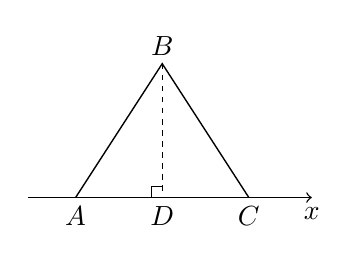
\begin{tikzpicture}[scale=1,line width=0.5pt]
\draw[->] (-0.4,0) -- (3.2,0) node[below] {$x$};
\draw (0.2,0) -- (1.3,1.7) -- (2.4,0);
\node at (0.2,-0.24) {$A$};
\node at (1.3,-0.24) {$D$};
\node at (2.4,-0.24) {$C$};
\node at (1.3,1.92) {$B$};
\draw[dash pattern=on 2pt off 2pt] (1.3,1.7) -- (1.3,0);
\draw (1.16,0) -- (1.16,0.14) -- (1.3,0.14);
\end{tikzpicture}
\end{center}
\step{$AB=AC=BC=\dfrac{2\sqrt3}3$，则 $x_2=x_1+AD=x_1+\dfrac{\sqrt3}3$，$x_3=x_1+\dfrac{2\sqrt3}3$，}
\step{存在 $x_1=-\dfrac{\sqrt3}3$，使得 $x_2=x_1+\dfrac{\sqrt3}3=0\in\Q$，且 $x_3=x_1+\dfrac{2\sqrt3}3=\dfrac{\sqrt3}3$ 为无理数，}
\step{即 $D(x_2)=1$，$D(x_3)=0$ 与图形一致，符合题意，}
\step{此时，$S_{\triangle ABC}=\dfrac12AC\cdot BD=\dfrac{\sqrt3}3$.}
\step{综上所述，存在这样的点 $A$、$B$、$C$，该正三角形的面积为 $\dfrac{\sqrt3}3$.}
\solend

\fi

\item 已知函数 $f(x)$ 满足：对 $\forall x\in R$，都有 $f(x+2025)\leqslant f(x)+2026$，
$f(x+2026)\geqslant f(x)+2027$，若 $f(1)=0$，则 $f(2)$ 的取值范围是\blankline[4.4em].

\ifanswer
\solbegin
\step{对 $\forall x\in R$，都有 $f(x+2025)\leqslant f(x)+2026$，$f(x+2026)\geqslant f(x)+2027$，}
\step{则 $f(x)+2027\leqslant f(x+2026)=f(x+1+2025)\leqslant f(x+1)+2026$，}
\step{即 $f(x)+1\leqslant f(x+1)$，所以 $f(2)\geqslant f(1)+1=1$；}
\step{$f(x)+2026\geqslant f(x+2025)=f(x+2024+1)\geqslant f(x+2024)+1$}
\step{$\geqslant\cdots\geqslant f(x+1)+2024$，所以 $f(x)+2\geqslant f(x+1)$，}
\step{所以 $f(2)\leqslant f(1)+2=2$；}
\step{即 $f(2)$ 的取值范围是 $[1,2]$.}
\solend

\fi

\end{enumerate}

\bigsec{二、选择题}

\begin{enumerate}
\setcounter{enumi}{12}

\item 若实数 $0<m<n<1$，而实数 $x>1$，则下列不等式正确的是\mbox{（\quad）}

\keepwithprev
A. $m^x<n^x$\qquad\qquad B. $x^m>x^n$\qquad\qquad C. $\log_xm>\log_xn$\qquad D. $\log_mx<\log_nx$

\ifanswer
\solbegin
\step{对于 $A$，函数 $f(t)=t^x$ 是以 $t$ 为变量，$x$ 为常量的幂函数，}
\step{由于 $x>1$，易得 $f(t)$ 在 $(0,+\infty)$ 上严格增，}
\step{$0<m<n<1$，$x>1$，可以得到 $m^x<n^x$，故 $A$ 正确；}
\step{对于 $B$，函数 $g(s)=x^s$，是以 $s$ 为变量，$x$ 为常量的指数函数，}
\step{由于 $x>1$，则 $g(s)$ 严格增，$0<m<n<1$，可以得到 $x^m<x^n$，故 $B$ 不正确；}
\step{对于 $C$，$\log_xm=\dfrac{\lg m}{\lg x}$，$\log_xn=\dfrac{\lg n}{\lg x}$，由于 $0<m<n<1$，则 $\lg m<\lg n<0$，}
\step{$x>1$，则 $\lg x>0$，则有 $\dfrac{\lg m}{\lg x}<\dfrac{\lg n}{\lg x}$，即 $\log_xm<\log_xn$，故 $C$ 不正确；}
\step{对于 $D$，由 $\log_mx-\log_nx=\dfrac{\lg x}{\lg m}-\dfrac{\lg x}{\lg n}=\dfrac{\lg x(\lg n-\lg m)}{\lg m\lg n}$，}
\step{因为实数 $0<m<n<1$，而实数 $x>1$，}
\step{所以 $\lg x>0$，$\lg m<\lg n<0$，则 $\dfrac{\lg x(\lg n-\lg m)}{\lg m\lg n}>0$，即 $\log_mx>\log_nx$，}
\step{故 $D$ 不正确.}
\step{故选 $A$.}
\solend

\fi

\item 已知 $x>1$，$y>1$，则 “$4^x>2^y$” 是 $\log_2x>\log_4(y-1)$ ”的\mbox{（\quad）}

\keepwithprev
A. 充分不必要条件\qquad\qquad B. 必要不充分条件

C. 充要条件\qquad\qquad D. 既不充分也不必要条件

\ifanswer
\solbegin
\step{因为 $x>1$，$y>1$，若 $4^x>2^y$，即 $2^{2x}>2^y$，所以 $2x>y>1$，}
\step{因为 $\dfrac y2-\sqrt{y-1}=\dfrac{(\sqrt{y-1})^2-2\sqrt{y-1}+1}2=\dfrac{(\sqrt{y-1}-1)^2}2\geqslant0$，}
\step{即 $\dfrac y2\geqslant\sqrt{y-1}>0$，所以 $\log_2\dfrac y2\geqslant\log_2\sqrt{y-1}=\dfrac12\log_2(y-1)=\log_4(y-1)$，}
\step{又 $x>\dfrac y2>\dfrac12$，所以 $\log_2x>\log_2\dfrac y2\geqslant\log_4(y-1)$，故充分性成立；}
\step{取 $x=2$，$y=4$，满足 $1=\log_2x>\log_4(y-1)=\log_43$，}
\step{但 $16=4^x=2^y=16$，即不满足 $4^x>2^y$，故必要性不成立.}% 链首链尾两个 16 系原卷笔误，应为 4^x=2^y=16，照录
\step{故选 $A$.}
\solend

\fi

\item 以下命题中，真命题的个数是\mbox{（\quad）}

①函数 $y=(x^2+1)^2+3$ 最小值为 3；②若 $2^a+\log_2a=4^b+2\log_4b$，则 $a<2b$；③不等式
$2^x-x-1>0$ 的解集为 $(1,+\infty)$.

\keepwithprev
A. $0$\qquad\qquad B. $1$\qquad\qquad C. $2$\qquad\qquad D. $3$

\ifanswer
\solbegin
\step{对于①，由于 $x^2+1\geqslant1$，则 $y=(x^2+1)^2+3\geqslant4$，}
\step{即函数 $y=(x^2+1)^2+3$ 最小值为 4，①错误；}
\step{对于②，由于 $b>0$，}
\step{则有 $2^a+\log_2a=4^b+2\log_4b=2^{2b}+\log_2b<2^{2b}+\log_22b$，}
\step{设 $f(x)=2^x+\log_2x$，易得 $f(x)$ 在 $(0,+\infty)$ 上为严格增函数，必有 $a<2b$，}
\step{②正确；}
\step{对于③，当 $x=-1$ 时，$2^x-x-1=2^x(x+1)>0$，即 $-1$ 在不等式的解集内，}
\step{③错误；}
\step{故选 $B$.}
\solend

\fi

\item 已知函数 $f(x)=ax^2+bx+c$（$a\neq0$ 且 $a<b$），若对任意的 $x\in R$，$f(x)\geqslant0$，且
$f(1)\geqslant\lambda(b-a)$，则实数 $\lambda$ 的取值范围为\mbox{（\quad）}

\keepwithprev
A. $(-\infty,2]$\qquad\qquad B. $[2\text{，}+\infty)$\qquad\qquad C. $(-\infty\text{，}3]$\qquad\qquad D. $[3\text{，}+\infty)$% 原卷 B/C/D 用全角逗号、A 用半角，照录

\ifanswer
\solbegin
\step{因为函数 $f(x)\geqslant0$ 恒成立，所以 $a>0$，且 $\Delta=b^2-4ac\leqslant0$，即 $c\geqslant\dfrac{b^2}{4a}$，}
\step{所以 $a+b+c\geqslant a+b+\dfrac{b^2}{4a}$，又 $a<b$，所以 $b-a>0$，}
\step{又 $f(1)\geqslant\lambda(b-a)$ 恒成立，所以 $a+b+c\geqslant\lambda(b-a)$ 恒成立，}
\step{即 $\lambda\leqslant\left(\dfrac{a+b+c}{b-a}\right)_{\min}=\dfrac{a+b+\dfrac{b^2}{4a}}{b-a}$，}
\step{令 $t=\dfrac ba$（$t>1$），则 $\dfrac{a+b+\dfrac{b^2}{4a}}{b-a}=\dfrac{1+t+\dfrac{t^2}4}{t-1}$，}
\step{令 $\mu=t-1$（$\mu>0$），则 $t=\mu+1$，}
\step{故上式 $=\dfrac{1+\mu+1+\dfrac{(\mu+1)^2}4}{\mu}=\dfrac14\left(\mu+\dfrac9\mu+6\right)$，}
\step{对 $\mu>0$，有 $\mu+\dfrac9\mu\geqslant2\sqrt{\mu\times\dfrac9\mu}=6$，当且仅当 $\mu=\dfrac9\mu$，即 $\mu=3$ 时取等号，}
\step{所以 $\dfrac14\left(\mu+\dfrac9\mu+6\right)\geqslant\dfrac14(6+6)=3$，故 $\lambda\leqslant3$，}
\step{即实数 $\lambda$ 的取值范围为 $(-\infty,3]$. 故选 $C$.}
\solend

\fi

\end{enumerate}

\bigsec{三、解答题}

\begin{enumerate}
\setcounter{enumi}{16}

\item 已知函数 $f(x)=\log_\frac23(ax^2-6x+18)$.

（1）若 $f(x)$ 的定义域为 $R$，求实数 $a$ 的取值范围.

（2）若 $f(x)$ 的值域为 $R$，求实数 $a$ 的取值范围.

\ansspace*[10]

\ifanswer
\solbegin
\stepm{（1）}{由 $f(x)=\log_\frac23(ax^2-6x+18)$ 的定义域为 $R$，得 $ax^2-6x+18>0$ 恒成立，}
\step{$a=0$ 时，$f(x)=\log_\frac23(18-6x)$ 的定义域为 $(-\infty,3)$，不符合题意.}
\step{$a\neq0$ 时，$\begin{cases}a>0\\ \Delta=36-4\times18a<0\end{cases}$，解得 $a>\dfrac12$.}
\step{综上，$a$ 的取值范围是 $\left(\dfrac12,+\infty\right)$.}
\stepm{（2）}{$a=0$ 时，$f(x)=\log_\frac23(18-6x)$ 的值域为 $R$，符合题意.}
\step{$a\neq0$ 时，$\begin{cases}a>0\\ \Delta=36-4\times18a\geqslant0\end{cases}$，解得 $0<a\leqslant\dfrac12$.}
\step{综上，$a$ 的取值范围是 $\left[0,\dfrac12\right]$.}
\solend

\fi

\item 已知 $f(x)=\log_ax+\log_a(6-x)$，$a>0$ 且 $a\neq1$，且 $f(3)=2$.

（1）求 $a$ 的值及 $f(x)$ 的单调区间.

（2）若对于 $\forall x_1\in(0,6)$，$\exists x_2\in[1,9]$，使得 $f(x_1)\leqslant t+\log_3x_2$ 成立，求实数 $t$ 的取值范
围.

\ansspace*[12]

\ifanswer
\solbegin
\stepm{（1）}{已知 $f(x)=\log_ax+\log_a(6-x)$，且 $f(3)=2$.}
\step{得 $\log_a3+\log_a(6-3)=2$，即 $2\log_a3=2$，}
\step{因此 $\log_a3=1$，因此 $a=3$，因此 $f(x)=\log_3x+\log_3(6-x)$，}
\step{因为 $\begin{cases}x>0\\ 6-x>0\end{cases}$，因此 $0<x<6$，故 $f(x)$ 的定义域为 $(0,6)$；}
\step{$f(x)=\log_3(6x-x^2)$，}
\step{因为函数 $y=6x-x^2$ 在 $(0,3)$ 上严格增，在 $(3,6)$ 上严格减，}
\step{又函数 $y=\log_3x$ 为严格增函数，}
\step{由复合函数的单调性得函数 $f(x)$ 在 $(0,3)$ 上严格增，在 $(3,6)$ 上严格减；}
\stepm{（2）}{令 $g(x)=t+\log_3x$，}
\step{因为 $\forall x_1\in(0,6)$，$\exists x_2\in[1,9]$，使得 $f(x_1)\leqslant t+\log_3x_2$，}
\step{即 $f(x_{1})_{\max}\leqslant g(x_{2})_{\max}$，}
\step{其中由（1）得 $f(x_{1})_{\max}=f(3)=2$.}
\step{又 $g(x)=t+\log_3x$ 在 $[1,9]$ 上严格增，因此 $g(x)_{\max}=g(9)=t+2$，}
\step{因此 $2\leqslant t+2$，因此实数 $t$ 的取值范围为 $[0,+\infty)$.}
\solend

\fi

\item 某心理学研究小组在对学生上课注意力集中情况的调查研究中，发现其注意力指数 $p$ 与
听课时间 $t$ 之间的关系满足如图所示的曲线. 当 $t\in(0,14]$ 时，曲线是二次函数图象的一部
分，当 $t\in[14,40]$ 时，曲线是函数 $y=\log_a(t-5)+83$（$a>0$ 且 $a\neq1$）图象的一部分. 根据
专家研究，当注意力指数 $p$ 大于等于 80 时听课效果最佳.

（1）试求 $p=f(t)$ 的函数关系式；

（2）当一位学生在坚持听课 32 分钟时，注意力指数 $p$ 大约为多少？

（3）一道数学难题，讲解需要 20 分钟，问老师能否经过合理安排在学生听
课效果最佳时讲完？请说明理由.

\begin{center}
% 原图第 9 页题干 p-t 曲线图按原图形状用 TikZ 重排（三版都出）。
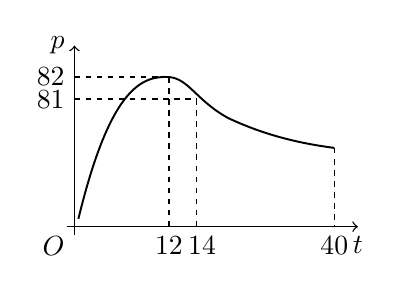
\begin{tikzpicture}[scale=1,line width=0.5pt]
\draw[->] (-0.1,0) -- (3.6,0) node[below] {$t$};
\draw[->] (0,-0.1) -- (0,2.3) node[left] {$p$};
\node[below left] at (0,0) {$O$};
\draw[line width=0.7pt] (0.05,0.1) .. controls (0.45,1.75) and (0.85,1.92) .. (1.2,1.9)
  .. controls (1.45,1.88) and (1.55,1.6) .. (1.95,1.38)
  .. controls (2.5,1.12) and (3.0,1.04) .. (3.3,1.0);
\draw[dash pattern=on 2pt off 2pt] (0,1.9) -- (1.2,1.9);
\draw[dash pattern=on 2pt off 2pt] (0,1.62) -- (1.55,1.62);
\draw[dash pattern=on 2pt off 2pt] (1.2,1.9) -- (1.2,0);
\draw[dash pattern=on 2pt off 2pt] (1.55,1.62) -- (1.55,0);
\draw[dash pattern=on 2pt off 2pt] (3.3,1.0) -- (3.3,0);
\node[left] at (0,1.9) {$82$};
\node[left] at (0,1.62) {$81$};
\node[below] at (1.2,0) {$12$};
\node[below] at (1.62,0) {$14$};
\node[below] at (3.3,0) {$40$};
\end{tikzpicture}
\end{center}

\ansspace*[12]

\ifanswer
\solbegin
\stepm{（1）}{由题意得当 $t\in(0,14]$ 时，设 $f(t)=c(t-12)^2+82$（$c<0$），}
\step{又 $f(14)=81$，所以 $c(14-12)^2+82=81$，解得 $c=-\dfrac14$；}
\step{所以 $f(t)=-\dfrac14(t-12)^2+82$,$t\in(0,14]$；}
\step{又当 $t\in[14,40]$ 时，函数 $y=\log_a(t-5)+83$（$a>0$ 且 $a\neq1$），}
\step{又当 $x=14$ 时，$y=81$，所以 $81=\log_a(14-5)+83$，解得 $a=\dfrac13$；}
\step{所以 $f(t)=\log_\frac13(t-5)+83$,$t\in[14,40]$，}
\step{所以 $p=\begin{cases}-\dfrac14(t-12)^2+82, & t\in(0,14]\\ \log_\frac13(t-5)+83, & t\in(14,40]\end{cases}$；}
\stepm{（2）}{当 $t=32$ 时，$p=\log_\frac13(32-5)+83=80$，}
\step{所以当一位学生在坚持听课 32 分钟时，注意力指数 $p$ 大约为 80；}
\stepm{（3）}{当 $t\in(0,14]$ 时，$-\dfrac14(t-12)^2+82\geqslant80$，解得 $t\in[12-2\sqrt2,14]$，}
\step{当 $t\in[14,40]$ 时，$\log_\frac13(t-5)+83\geqslant80$，解得 $5<t\leqslant32$，则 $t\in[14,32]$，}
\step{因此当 $t\in[12-2\sqrt2,32]$ 时学生听课效果最佳，}
\step{此时 $\Delta t=32-(12-2\sqrt2)=20+2\sqrt2>20$，}
\step{所以老师能经过合理安排时间在学生听课效果最佳时段讲完.}
\solend

\fi

\item 已知 $a\in R$，函数 $f(x+1)=\log_2\left(\dfrac{ax+1+a}{x+1}\right)$.

（1）若 $a=2$，求函数 $f(x)$ 的表达式及定义域；

（2）若关于 $x$ 的方程 $f\left(\dfrac x2\right)-\log_2[(a-2)x+3a-5]=0$ 的解集中恰好只有一个元素，求实
数 $a$ 的取值范围.

\ansspace*[14]

\ifanswer
\solbegin
\stepm{（1）}{$f(x+1)=\log_2\left(\dfrac{ax+1+a}{x+1}\right)$，}
\step{令 $x+1=t$，则 $f(t)=\log_2\left(\dfrac1t+a\right)$，即 $f(x)=\log_2\left(\dfrac1x+a\right)$，}
\step{因为 $a=2$，所以 $f(x)=\log_2\left(2+\dfrac1x\right)$，}
\step{由 $2+\dfrac1x>0$ 得定义域为 $\left(-\infty,-\dfrac12\right)\cup(0,+\infty)$；}
\stepm{（2）}{由（1）得 $f(x)=\log_2\left(\dfrac1x+a\right)$，}
\step{方程 $f\left(\dfrac x2\right)-\log_2[(a-2)x+3a-5]=0$，}
\step{即 $\log_2\left(\dfrac2x+a\right)-\log_2[(a-2)x+3a-5]=0$，}
\step{可转化为 $(a-2)x^2+(2a-5)x-2=0$，且 $\dfrac2x+a>0$.}
\step{①当 $a-2=0$，即 $a=2$ 时，$x=-2$，符合题意；}
\step{②当 $a-2\neq0$，即 $a\neq2$ 时，$x_1=-2$,$x_2=\dfrac1{a-2}$，}
\step{（$i$）当 $-2=\dfrac1{a-2}$ 时，即 $a=\dfrac32$ 时，符合题意；}
\step{（$ii$）当 $-2\neq\dfrac1{a-2}$ 时，即 $a\neq\dfrac32$ 且 $a\neq2$ 时，}
\step{要满足题意，则有 $\begin{cases}-1+a>0\\ 3a-4\leqslant0\end{cases}\Rightarrow1<a\leqslant\dfrac43$ 或 $\begin{cases}-1+a\leqslant0\\ 3a-4>0\end{cases}$，无解；}
\step{综上，$a$ 的取值范围 $\left(1,\dfrac43\right]\cup\left\{2,\dfrac32\right\}$.}
\solend

\fi

\item 已知函数 $y=f(x)$ 是定义在 $[0,+\infty)$ 上的函数，并且 $f(x)\geqslant0$，对于定义域内的任意自
变量的值 $x$、$y$，满足 $f(y)f(x^2f(y)+xf(y))=f(x^2+y+x)$，$f(a)=0$，其中
$a>0$.

（1）当 $f(0)\neq0$ 时，求 $f(0)$；

（2）已知当 $0\leqslant x<a$ 时，有 $f(x)\neq0$.

（$i$）求 $f(a+3)$；

（$ii$）求函数 $y=f(x)$ 的解析式（用 $a$ 表示）.

\ansspace*[16]

\ifanswer
\solbegin
\stepm{（1）}{因为 $f(x)\geqslant0$，且对于定义域内的任意自变量的值 $x$、$y$，}
\step{满足 $f(y)f(x^2f(y)+xf(y))=f(x^2+y+x)$，}
\step{令 $x=y=0$，则 $f^2(0)=f(0)$，因为 $f(0)\neq0$，所以 $f(0)=1$，}
\stepm{（2）}{（$i$）由 $f(y)f(x^2f(y)+xf(y))=f(x^2+y+x)$，}
\step{得 $f(y)f[(x^2+x)f(y)]=f[(x^2+x)+y]$，}
\step{令 $t=x^2+x$，因为 $x\geqslant0$，所以 $t=x^2+x\in[0,+\infty)$，}
\step{所以有 $f(y)f(tf(y))=f(t+y)$，因为 $f(a)=0$，}
\step{令 $y=a$，$t=3$，得 $f(a+3)=f(a)f(3f(a))=0\times f(3f(a))=0$；}
\step{（$ii$）当 $x\geqslant a$ 时，令 $y=a$，$t=x-a$，}
\step{$f(x)=f(x-a+a)=f(a)f[(x-a)f(a)]=0$.}
\step{当 $0\leqslant x<a$ 时，则有 $0<a-x\leqslant a$，令 $y=x$，$t=a-x$，}
\step{则 $f(a)=f(a-x+x)=f(x)f[(a-x)f(x)]=0$.}
\step{因为 $f(x)\neq0$，所以有 $f((a-x)f(x))=0$，则 $(a-x)f(x)\geqslant a$，}
\step{又因为 $a-x>0$，即 $f(x)\geqslant\dfrac a{a-x}$.}
\step{令 $t=\dfrac a{f(x)}>0$,$y=x>0$，}
\step{则 $f\left(\dfrac a{f(x)}+x\right)=f(x)\cdot f\left(\dfrac a{f(x)}\cdot f(x)\right)=f(x)\cdot f(a)=0$，}
\step{所以有 $\dfrac a{f(x)}+x\geqslant a$，即 $\dfrac a{f(x)}\geqslant a-x$，得 $f(x)\leqslant\dfrac a{a-x}$，}
\step{所以当 $0\leqslant x<a$ 时，$f(x)=\dfrac a{a-x}$.}
\step{综上，$f(x)=\begin{cases}\dfrac a{a-x}, & 0\leqslant x<a\\ 0, & x\geqslant a\end{cases}$.}
\solend

\fi

\end{enumerate}

\end{document}
"
%
% 原始材料：微信公众号“魔都数学加油站”文章，作者破晓，2026-11-02 17:41 发布；
% 连载“27学年高一105”，原文标题“27学年高一105——2026-2027年上海市交附闵行高一上周末作业10.30”；
% 原文链接：https://mp.weixin.qq.com/s/XUfNEvGHjD0CB5jdoleBWw。
% 正文为 13 张 PNG 页（第 4、9、13 页 2560×3620，其余 4762×6735），题目下印有【解析】，为讲评版。
% 题目、解析均据原图转录；卷面水印及公众号页脚未录入。
%
% 卷首标题：原卷印作“2026-2027 年交附闵行高一上周末作业 10.30”（公众号标题中的“上海市”
% 卷面标题行没有，本稿照卷面），年份区间按全稿惯例排 en dash；原卷未印副标题，本稿按题目
% 内容标为“函数、不等式”（主体为指数与对数，第 3 题集合、第 16 题基本不等式）。
%
% 与原卷的排版差异：
%   ① 原文从第 3 题起，填空题编号为 3—12、选择题为 13—16、解答题为 17—21，本稿保留原题号；
%   ② 原卷每题下直接印【解析】，本稿按全稿惯例将解析置于答案版；选择题括号内未印答案，另由
%      解析末句“故选 X”给出；
%   ③ 原卷未印副标题，本稿按“知识模块”口径补出；
%   ④ 原卷填空横线按全稿惯例排为 \blankline[4.4em]；解答题按惯例加 \ansspace；选择题括号排
%      \mbox{（\quad）}、选项段前按惯例加 \keepwithprev；
%   ⑤ $f(x_1)_{max}$、$g(x)_max$、$\left(\frac{a+b+c}{b-a}\right)_{min}$ 等下标原卷排斜体，
%      按 高一96 成例改正体 $\max$、$\min$；
%   ⑥ 原卷数集排斜体 $R$／$Q$，按全稿惯例改 $\R$／$\Q$；
%   ⑦ 第 11 题解析的两幅三角形示意图与第 19 题题干的 $p$-$t$ 曲线图均按原图形状用 TikZ 重排
%      （第 19 题图属题干、三版都出；第 11 题图属解析、仅答案版显示）。
%
% 原卷存疑／笔误（均照录加注）：
%   第 14 题解析“但 $16=4^x=2^y=16$”（链首、链尾的两个 $16$ 系原卷笔误，按上下文应为
%   $4^x=2^y=16$）；
%   第 16 题选项的区间分隔逗号 A 项排半角、B／C／D 三项排全角（原卷自身不一致）；
%   第 21 题 (2) 的小问号排“（$i$）求…”（右括号紧贴“求”字），照录。
%
% 行数核对：逐题数 \step/\stepm 条数，合计 159 条（Q3：2；Q4：1；Q5：4；Q6：6；Q7：3；
% Q8：7；Q9：5；Q10：3；Q11：15；Q12：7；Q13：12；Q14：7；Q15：9；Q16：10；Q17：7；
% Q18：14；Q19：14；Q20：14；Q21：19），与原卷印刷行逐题相等。
%
\documentclass[a4paper,11pt]{article}
\usepackage{common}

\begin{document}

\examtitlest[3]{2026--2027 年交附闵行高一上周末作业 10.30}{函数、不等式}

\bigsec{一、填空题}

\begin{enumerate}
\setcounter{enumi}{2}

\item 已知集合 $M=\{1,m\}$，$N=\{n,\log_2n\}$，若 $M=N$，则 $(m-n)^{2027}=$\blankline[4.4em].

\ifanswer
\solbegin
\step{由题意得 $\begin{cases}n=1\\ \log_2n=m\end{cases}$ 或 $\begin{cases}n=m\\ \log_2n=1\end{cases}$，解得 $\begin{cases}n=1\\ m=0\end{cases}$ 或 $\begin{cases}n=2\\ m=2\end{cases}$，}
\step{所以 $(m-n)^{2027}=-1$ 或 $0$.}
\solend

\fi

\item 已知 $\log_{2x^2-1}(3x^2+2x-1)=1$，则 $x=$\blankline[4.4em].

\ifanswer
\solbegin
\step{因为 $\log_{2x^2-1}(3x^2+2x-1)=1$，所以 $\begin{cases}2x^2-1>0\\ 2x^2-1\neq1\\ 3x^2+2x-1>0\\ 2x^2-1=3x^2+2x-1\end{cases}$，解得 $x=-2$.}
\solend

\fi

\item 已知 $m>1$，$n>1$，$\lg m=\log_n100$，则 $mn$ 的最小值为\blankline[4.4em].

\ifanswer
\solbegin
\step{由 $m>1$，$n>1$，得 $\lg m>0$，$\lg n>0$，}
\step{因为 $\lg m=\log_n100=\dfrac{\lg100}{\lg n}=\dfrac2{\lg n}$，所以 $\lg m\cdot\lg n=2$，}
\step{所以 $\lg(mn)=\lg m+\lg n\geqslant2\sqrt{\lg m\cdot\lg n}=2\sqrt2$，}
\step{当且仅当 $m=n=10^{\sqrt2}$ 时取等号，则 $mn\geqslant10^{2\sqrt2}$，即 $mn$ 的最小值为 $10^{2\sqrt2}$.}
\solend

\fi

\item 设 $m$、$n$ 分别是方程 $\log_{2013}x+x-9=0$ 和 $2013^x+x-9=0$ 的根，则 $m+n=$\blankline[4.4em].

\ifanswer
\solbegin
\step{由 $\log_{2013}x+x-9=0$，得 $\log_{2013}x=-x+9$，}
\step{因为 $m$ 是方程 $\log_{2013}x+x-9=0$ 的根，}
\step{所以 $m$ 为函数 $y=\log_{2013}x$ 与 $y=-x+9$ 图象交点的横坐标，}
\step{同理 $n$ 是函数 $y=2013^x$ 与 $y=-x+9$ 图象交点的横坐标，}
\step{因为 $y=\log_{2013}x$ 与 $y=2013^x$ 互为反函数，其图象关于直线 $y=x$ 对称，}
\step{联立 $\begin{cases}y=-x+9\\ y=x\end{cases}$，解得 $x=\dfrac92$，所以 $m+n=\dfrac92\times2=9$.}
\solend

\fi

\item 已知函数 $f(x)=\dfrac1{\log_2(x^2+4)}$，则 $f(-2)=$\blankline[2em]，$f(x)$ 的值域为\blankline[4.4em].

\ifanswer
\solbegin
\step{$f(-2)=\dfrac1{\log_28}=\dfrac13$.}
\step{因为 $x^2+4\geqslant4$，所以 $\log_2(x^2+4)\geqslant\log_24=2$，所以 $0<\dfrac1{\log_2(x^2+4)}\leqslant\dfrac12$，}
\step{故 $f(x)$ 的值域为 $\left(0,\dfrac12\right]$.}
\solend

\fi

\item 已知 $\alpha$、$\beta$ 是方程 $9^x-2m\cdot3^x+m^2-1=0$ 的两个根，若 $\alpha+\beta=1$，则 $\alpha\beta=$\blankline[4.4em].

\ifanswer
\solbegin
\step{由题意得方程 $9^x-2m\cdot3^x+m^2-1=0$ 有两个根，}
\step{则方程 $t^2-2mt+m^2-1=0$ 有二正根，}
\step{则 $\begin{cases}\Delta=4m^2-4(m^2-1)\geqslant0\\ 2m>0\\ m^2-1>0\end{cases}$，解得 $m>1$，}
\step{又 $\alpha$、$\beta$ 是方程 $9^x-2m\cdot3^x+m^2-1=0$ 的两个根，}
\step{则 $3^\alpha\times3^\beta=m^2-1$，又 $\alpha+\beta=1$，则 $m^2-1=3^{\alpha+\beta}=3$，}
\step{解得 $m=2$ 或 $m=-2$（舍），则 $3^\alpha+3^\beta=2m=4$，又 $\alpha=1-\beta$，}
\step{则 $3^{1-\beta}+3^\beta=4$，解得 $\beta=0$ 或 $\beta=1$，则 $\begin{cases}\alpha=1\\ \beta=0\end{cases}$ 或 $\begin{cases}\alpha=0\\ \beta=1\end{cases}$，则 $\alpha\beta=0$.}
\solend

\fi

\item 已知 $a>b>0$，$\ln a=2\ln b$，且 $a\lg b=b\lg a$，则 $a+b=$\blankline[4.4em].

\ifanswer
\solbegin
\step{因为 $a>b>0$，$\ln a=2\ln b=\ln b^2$，所以 $a=b^2$，}
\step{由 $a\lg b=b\lg a$ 得 $b^2\lg b=b\lg b^2$，即 $b\lg b=2\lg b$，所以 $b=1$ 或 $b=2$，}
\step{当 $b=2$，$a=4$，满足题意，}
\step{当 $b=1$ 时，$a=1$ 与 $a>b>0$ 矛盾，所以 $b=1$ 舍去，}
\step{所以 $a+b=6$.}
\solend

\fi

\item 函数 $f(x)=\begin{cases}2^x, & x\leqslant t\\ \log_\frac12x, & x>t\end{cases}$ 的值域为 $M$，且 $8\notin M$，则实数 $t$ 的取值集合为\blankline[4.4em].

\ifanswer
\solbegin
\step{当 $x\leqslant t$ 时，函数 $f(x)=2^x$ 在 $(-\infty,t]$ 严格增，}
\step{当 $x>t$ 时，$f(x)=\log_\frac12x$ 在 $(t,+\infty)$ 严格减，}
\step{若 $8\notin M$，则满足条件 $\begin{cases}2^t<8\\ \log_\frac12t\leqslant8\end{cases}\Rightarrow\dfrac1{256}\leqslant t<3$，故实数 $t$ 的取值集合为 $\left[\dfrac1{256},3\right)$.}
\solend

\fi

\item 德国数学家狄利克雷在数学领域成就显著，以其命名函数 $D(x)=\begin{cases}1, & x\text{为有理数}\\ 0, & x\text{为无理数}\end{cases}$，该函
数被称为狄利克雷函数。那么是否存在三个点 $A(x_1,D(x_1))$、$B(x_2,D(x_2))$、$C(x_3,D(x_3))$，
使得 $\triangle ABC$ 为等边三角形，若不存在请在横线上填写“不存在”，如果存在则在横线上填写
该正三角形的面积\blankline[4.4em].

\ifanswer
\solbegin
\step{因为 $D(x)=\begin{cases}1, & x\text{为有理数}\\ 0, & x\text{为无理数}\end{cases}$，所以 $D(x)=0$ 或 1，}
\step{设存在三个点 $A(x_1,D(x_1))$、$B(x_2,D(x_2))$、$C(x_3,D(x_3))$，}
\step{使得 $\triangle ABC$ 为等边三角形，则 $D(x_1)$、$D(x_2)$、$D(x_3)$ 不同时为 0 或 1，}
\step{不妨设 $x_1<x_2<x_3$，分析得 $\triangle ABC$ 的位置有两种情况，}
\step{第一种情况：当 $x_1$ 为有理数时，即 $D(x_1)=1$，如图，过点 $B$ 作 $BD\perp AC$，}
\begin{center}
% 原图第 4 页解析示意图按原图形状用 TikZ 重排（第一种情况：$B$ 在 $x$ 轴上、$AC$ 在上方）。
\begin{tikzpicture}[scale=1,line width=0.5pt]
\draw (0,1.2) -- (2.6,1.2);
\node at (0.25,1.4) {$A$};
\node at (1.3,1.4) {$D$};
\node at (2.35,1.4) {$C$};
\draw[dash pattern=on 2pt off 2pt] (1.3,1.2) -- (1.3,0);
\draw (1.16,1.2) -- (1.16,1.06) -- (1.3,1.06);
\draw[->] (-0.5,0) -- (3.1,0) node[below] {$x$};
\node at (1.3,-0.24) {$B$};
\end{tikzpicture}
\end{center}
\step{垂足为 $D$，得 $BD=1$，$AD=\dfrac{\sqrt3}3$，$AB=AC=BC=\dfrac{2\sqrt3}3$，}
\step{则 $x_2=x_1+AD=x_1+\dfrac{\sqrt3}3$ 为无理数，$x_3=x_1+\dfrac{2\sqrt3}3$ 为无理数，}
\step{即 $D(x_2)=0$，$D(x_3)=0$ 与图形不一致，舍去；}
\step{第二种情况：当 $x_1$ 为无理数时，即 $D(x_1)=0$，如图，}
\step{过点 $B$ 作 $BD\perp AC$，垂足为 $D$，得 $BD=1$，$AD=\dfrac{\sqrt3}3$，}
\begin{center}
% 原图第 4 页解析示意图按原图形状用 TikZ 重排（第二种情况：$B$ 在上方、$AC$ 在 $x$ 轴上）。
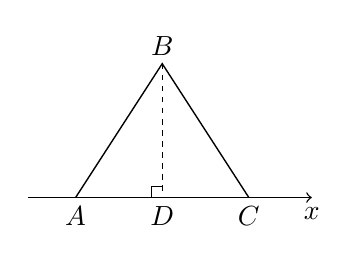
\begin{tikzpicture}[scale=1,line width=0.5pt]
\draw[->] (-0.4,0) -- (3.2,0) node[below] {$x$};
\draw (0.2,0) -- (1.3,1.7) -- (2.4,0);
\node at (0.2,-0.24) {$A$};
\node at (1.3,-0.24) {$D$};
\node at (2.4,-0.24) {$C$};
\node at (1.3,1.92) {$B$};
\draw[dash pattern=on 2pt off 2pt] (1.3,1.7) -- (1.3,0);
\draw (1.16,0) -- (1.16,0.14) -- (1.3,0.14);
\end{tikzpicture}
\end{center}
\step{$AB=AC=BC=\dfrac{2\sqrt3}3$，则 $x_2=x_1+AD=x_1+\dfrac{\sqrt3}3$，$x_3=x_1+\dfrac{2\sqrt3}3$，}
\step{存在 $x_1=-\dfrac{\sqrt3}3$，使得 $x_2=x_1+\dfrac{\sqrt3}3=0\in\Q$，且 $x_3=x_1+\dfrac{2\sqrt3}3=\dfrac{\sqrt3}3$ 为无理数，}
\step{即 $D(x_2)=1$，$D(x_3)=0$ 与图形一致，符合题意，}
\step{此时，$S_{\triangle ABC}=\dfrac12AC\cdot BD=\dfrac{\sqrt3}3$.}
\step{综上所述，存在这样的点 $A$、$B$、$C$，该正三角形的面积为 $\dfrac{\sqrt3}3$.}
\solend

\fi

\item 已知函数 $f(x)$ 满足：对 $\forall x\in R$，都有 $f(x+2025)\leqslant f(x)+2026$，
$f(x+2026)\geqslant f(x)+2027$，若 $f(1)=0$，则 $f(2)$ 的取值范围是\blankline[4.4em].

\ifanswer
\solbegin
\step{对 $\forall x\in R$，都有 $f(x+2025)\leqslant f(x)+2026$，$f(x+2026)\geqslant f(x)+2027$，}
\step{则 $f(x)+2027\leqslant f(x+2026)=f(x+1+2025)\leqslant f(x+1)+2026$，}
\step{即 $f(x)+1\leqslant f(x+1)$，所以 $f(2)\geqslant f(1)+1=1$；}
\step{$f(x)+2026\geqslant f(x+2025)=f(x+2024+1)\geqslant f(x+2024)+1$}
\step{$\geqslant\cdots\geqslant f(x+1)+2024$，所以 $f(x)+2\geqslant f(x+1)$，}
\step{所以 $f(2)\leqslant f(1)+2=2$；}
\step{即 $f(2)$ 的取值范围是 $[1,2]$.}
\solend

\fi

\end{enumerate}

\bigsec{二、选择题}

\begin{enumerate}
\setcounter{enumi}{12}

\item 若实数 $0<m<n<1$，而实数 $x>1$，则下列不等式正确的是\mbox{（\quad）}

\keepwithprev
A. $m^x<n^x$\qquad\qquad B. $x^m>x^n$\qquad\qquad C. $\log_xm>\log_xn$\qquad D. $\log_mx<\log_nx$

\ifanswer
\solbegin
\step{对于 $A$，函数 $f(t)=t^x$ 是以 $t$ 为变量，$x$ 为常量的幂函数，}
\step{由于 $x>1$，易得 $f(t)$ 在 $(0,+\infty)$ 上严格增，}
\step{$0<m<n<1$，$x>1$，可以得到 $m^x<n^x$，故 $A$ 正确；}
\step{对于 $B$，函数 $g(s)=x^s$，是以 $s$ 为变量，$x$ 为常量的指数函数，}
\step{由于 $x>1$，则 $g(s)$ 严格增，$0<m<n<1$，可以得到 $x^m<x^n$，故 $B$ 不正确；}
\step{对于 $C$，$\log_xm=\dfrac{\lg m}{\lg x}$，$\log_xn=\dfrac{\lg n}{\lg x}$，由于 $0<m<n<1$，则 $\lg m<\lg n<0$，}
\step{$x>1$，则 $\lg x>0$，则有 $\dfrac{\lg m}{\lg x}<\dfrac{\lg n}{\lg x}$，即 $\log_xm<\log_xn$，故 $C$ 不正确；}
\step{对于 $D$，由 $\log_mx-\log_nx=\dfrac{\lg x}{\lg m}-\dfrac{\lg x}{\lg n}=\dfrac{\lg x(\lg n-\lg m)}{\lg m\lg n}$，}
\step{因为实数 $0<m<n<1$，而实数 $x>1$，}
\step{所以 $\lg x>0$，$\lg m<\lg n<0$，则 $\dfrac{\lg x(\lg n-\lg m)}{\lg m\lg n}>0$，即 $\log_mx>\log_nx$，}
\step{故 $D$ 不正确.}
\step{故选 $A$.}
\solend

\fi

\item 已知 $x>1$，$y>1$，则 “$4^x>2^y$” 是 $\log_2x>\log_4(y-1)$ ”的\mbox{（\quad）}

\keepwithprev
A. 充分不必要条件\qquad\qquad B. 必要不充分条件

C. 充要条件\qquad\qquad D. 既不充分也不必要条件

\ifanswer
\solbegin
\step{因为 $x>1$，$y>1$，若 $4^x>2^y$，即 $2^{2x}>2^y$，所以 $2x>y>1$，}
\step{因为 $\dfrac y2-\sqrt{y-1}=\dfrac{(\sqrt{y-1})^2-2\sqrt{y-1}+1}2=\dfrac{(\sqrt{y-1}-1)^2}2\geqslant0$，}
\step{即 $\dfrac y2\geqslant\sqrt{y-1}>0$，所以 $\log_2\dfrac y2\geqslant\log_2\sqrt{y-1}=\dfrac12\log_2(y-1)=\log_4(y-1)$，}
\step{又 $x>\dfrac y2>\dfrac12$，所以 $\log_2x>\log_2\dfrac y2\geqslant\log_4(y-1)$，故充分性成立；}
\step{取 $x=2$，$y=4$，满足 $1=\log_2x>\log_4(y-1)=\log_43$，}
\step{但 $16=4^x=2^y=16$，即不满足 $4^x>2^y$，故必要性不成立.}% 链首链尾两个 16 系原卷笔误，应为 4^x=2^y=16，照录
\step{故选 $A$.}
\solend

\fi

\item 以下命题中，真命题的个数是\mbox{（\quad）}

①函数 $y=(x^2+1)^2+3$ 最小值为 3；②若 $2^a+\log_2a=4^b+2\log_4b$，则 $a<2b$；③不等式
$2^x-x-1>0$ 的解集为 $(1,+\infty)$.

\keepwithprev
A. $0$\qquad\qquad B. $1$\qquad\qquad C. $2$\qquad\qquad D. $3$

\ifanswer
\solbegin
\step{对于①，由于 $x^2+1\geqslant1$，则 $y=(x^2+1)^2+3\geqslant4$，}
\step{即函数 $y=(x^2+1)^2+3$ 最小值为 4，①错误；}
\step{对于②，由于 $b>0$，}
\step{则有 $2^a+\log_2a=4^b+2\log_4b=2^{2b}+\log_2b<2^{2b}+\log_22b$，}
\step{设 $f(x)=2^x+\log_2x$，易得 $f(x)$ 在 $(0,+\infty)$ 上为严格增函数，必有 $a<2b$，}
\step{②正确；}
\step{对于③，当 $x=-1$ 时，$2^x-x-1=2^x(x+1)>0$，即 $-1$ 在不等式的解集内，}
\step{③错误；}
\step{故选 $B$.}
\solend

\fi

\item 已知函数 $f(x)=ax^2+bx+c$（$a\neq0$ 且 $a<b$），若对任意的 $x\in R$，$f(x)\geqslant0$，且
$f(1)\geqslant\lambda(b-a)$，则实数 $\lambda$ 的取值范围为\mbox{（\quad）}

\keepwithprev
A. $(-\infty,2]$\qquad\qquad B. $[2\text{，}+\infty)$\qquad\qquad C. $(-\infty\text{，}3]$\qquad\qquad D. $[3\text{，}+\infty)$% 原卷 B/C/D 用全角逗号、A 用半角，照录

\ifanswer
\solbegin
\step{因为函数 $f(x)\geqslant0$ 恒成立，所以 $a>0$，且 $\Delta=b^2-4ac\leqslant0$，即 $c\geqslant\dfrac{b^2}{4a}$，}
\step{所以 $a+b+c\geqslant a+b+\dfrac{b^2}{4a}$，又 $a<b$，所以 $b-a>0$，}
\step{又 $f(1)\geqslant\lambda(b-a)$ 恒成立，所以 $a+b+c\geqslant\lambda(b-a)$ 恒成立，}
\step{即 $\lambda\leqslant\left(\dfrac{a+b+c}{b-a}\right)_{\min}=\dfrac{a+b+\dfrac{b^2}{4a}}{b-a}$，}
\step{令 $t=\dfrac ba$（$t>1$），则 $\dfrac{a+b+\dfrac{b^2}{4a}}{b-a}=\dfrac{1+t+\dfrac{t^2}4}{t-1}$，}
\step{令 $\mu=t-1$（$\mu>0$），则 $t=\mu+1$，}
\step{故上式 $=\dfrac{1+\mu+1+\dfrac{(\mu+1)^2}4}{\mu}=\dfrac14\left(\mu+\dfrac9\mu+6\right)$，}
\step{对 $\mu>0$，有 $\mu+\dfrac9\mu\geqslant2\sqrt{\mu\times\dfrac9\mu}=6$，当且仅当 $\mu=\dfrac9\mu$，即 $\mu=3$ 时取等号，}
\step{所以 $\dfrac14\left(\mu+\dfrac9\mu+6\right)\geqslant\dfrac14(6+6)=3$，故 $\lambda\leqslant3$，}
\step{即实数 $\lambda$ 的取值范围为 $(-\infty,3]$. 故选 $C$.}
\solend

\fi

\end{enumerate}

\bigsec{三、解答题}

\begin{enumerate}
\setcounter{enumi}{16}

\item 已知函数 $f(x)=\log_\frac23(ax^2-6x+18)$.

（1）若 $f(x)$ 的定义域为 $R$，求实数 $a$ 的取值范围.

（2）若 $f(x)$ 的值域为 $R$，求实数 $a$ 的取值范围.

\ansspace*[10]

\ifanswer
\solbegin
\stepm{（1）}{由 $f(x)=\log_\frac23(ax^2-6x+18)$ 的定义域为 $R$，得 $ax^2-6x+18>0$ 恒成立，}
\step{$a=0$ 时，$f(x)=\log_\frac23(18-6x)$ 的定义域为 $(-\infty,3)$，不符合题意.}
\step{$a\neq0$ 时，$\begin{cases}a>0\\ \Delta=36-4\times18a<0\end{cases}$，解得 $a>\dfrac12$.}
\step{综上，$a$ 的取值范围是 $\left(\dfrac12,+\infty\right)$.}
\stepm{（2）}{$a=0$ 时，$f(x)=\log_\frac23(18-6x)$ 的值域为 $R$，符合题意.}
\step{$a\neq0$ 时，$\begin{cases}a>0\\ \Delta=36-4\times18a\geqslant0\end{cases}$，解得 $0<a\leqslant\dfrac12$.}
\step{综上，$a$ 的取值范围是 $\left[0,\dfrac12\right]$.}
\solend

\fi

\item 已知 $f(x)=\log_ax+\log_a(6-x)$，$a>0$ 且 $a\neq1$，且 $f(3)=2$.

（1）求 $a$ 的值及 $f(x)$ 的单调区间.

（2）若对于 $\forall x_1\in(0,6)$，$\exists x_2\in[1,9]$，使得 $f(x_1)\leqslant t+\log_3x_2$ 成立，求实数 $t$ 的取值范
围.

\ansspace*[12]

\ifanswer
\solbegin
\stepm{（1）}{已知 $f(x)=\log_ax+\log_a(6-x)$，且 $f(3)=2$.}
\step{得 $\log_a3+\log_a(6-3)=2$，即 $2\log_a3=2$，}
\step{因此 $\log_a3=1$，因此 $a=3$，因此 $f(x)=\log_3x+\log_3(6-x)$，}
\step{因为 $\begin{cases}x>0\\ 6-x>0\end{cases}$，因此 $0<x<6$，故 $f(x)$ 的定义域为 $(0,6)$；}
\step{$f(x)=\log_3(6x-x^2)$，}
\step{因为函数 $y=6x-x^2$ 在 $(0,3)$ 上严格增，在 $(3,6)$ 上严格减，}
\step{又函数 $y=\log_3x$ 为严格增函数，}
\step{由复合函数的单调性得函数 $f(x)$ 在 $(0,3)$ 上严格增，在 $(3,6)$ 上严格减；}
\stepm{（2）}{令 $g(x)=t+\log_3x$，}
\step{因为 $\forall x_1\in(0,6)$，$\exists x_2\in[1,9]$，使得 $f(x_1)\leqslant t+\log_3x_2$，}
\step{即 $f(x_{1})_{\max}\leqslant g(x_{2})_{\max}$，}
\step{其中由（1）得 $f(x_{1})_{\max}=f(3)=2$.}
\step{又 $g(x)=t+\log_3x$ 在 $[1,9]$ 上严格增，因此 $g(x)_{\max}=g(9)=t+2$，}
\step{因此 $2\leqslant t+2$，因此实数 $t$ 的取值范围为 $[0,+\infty)$.}
\solend

\fi

\item 某心理学研究小组在对学生上课注意力集中情况的调查研究中，发现其注意力指数 $p$ 与
听课时间 $t$ 之间的关系满足如图所示的曲线. 当 $t\in(0,14]$ 时，曲线是二次函数图象的一部
分，当 $t\in[14,40]$ 时，曲线是函数 $y=\log_a(t-5)+83$（$a>0$ 且 $a\neq1$）图象的一部分. 根据
专家研究，当注意力指数 $p$ 大于等于 80 时听课效果最佳.

（1）试求 $p=f(t)$ 的函数关系式；

（2）当一位学生在坚持听课 32 分钟时，注意力指数 $p$ 大约为多少？

（3）一道数学难题，讲解需要 20 分钟，问老师能否经过合理安排在学生听
课效果最佳时讲完？请说明理由.

\begin{center}
% 原图第 9 页题干 p-t 曲线图按原图形状用 TikZ 重排（三版都出）。
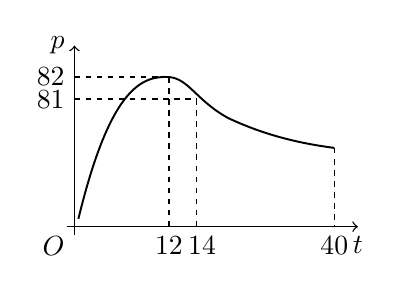
\begin{tikzpicture}[scale=1,line width=0.5pt]
\draw[->] (-0.1,0) -- (3.6,0) node[below] {$t$};
\draw[->] (0,-0.1) -- (0,2.3) node[left] {$p$};
\node[below left] at (0,0) {$O$};
\draw[line width=0.7pt] (0.05,0.1) .. controls (0.45,1.75) and (0.85,1.92) .. (1.2,1.9)
  .. controls (1.45,1.88) and (1.55,1.6) .. (1.95,1.38)
  .. controls (2.5,1.12) and (3.0,1.04) .. (3.3,1.0);
\draw[dash pattern=on 2pt off 2pt] (0,1.9) -- (1.2,1.9);
\draw[dash pattern=on 2pt off 2pt] (0,1.62) -- (1.55,1.62);
\draw[dash pattern=on 2pt off 2pt] (1.2,1.9) -- (1.2,0);
\draw[dash pattern=on 2pt off 2pt] (1.55,1.62) -- (1.55,0);
\draw[dash pattern=on 2pt off 2pt] (3.3,1.0) -- (3.3,0);
\node[left] at (0,1.9) {$82$};
\node[left] at (0,1.62) {$81$};
\node[below] at (1.2,0) {$12$};
\node[below] at (1.62,0) {$14$};
\node[below] at (3.3,0) {$40$};
\end{tikzpicture}
\end{center}

\ansspace*[12]

\ifanswer
\solbegin
\stepm{（1）}{由题意得当 $t\in(0,14]$ 时，设 $f(t)=c(t-12)^2+82$（$c<0$），}
\step{又 $f(14)=81$，所以 $c(14-12)^2+82=81$，解得 $c=-\dfrac14$；}
\step{所以 $f(t)=-\dfrac14(t-12)^2+82$,$t\in(0,14]$；}
\step{又当 $t\in[14,40]$ 时，函数 $y=\log_a(t-5)+83$（$a>0$ 且 $a\neq1$），}
\step{又当 $x=14$ 时，$y=81$，所以 $81=\log_a(14-5)+83$，解得 $a=\dfrac13$；}
\step{所以 $f(t)=\log_\frac13(t-5)+83$,$t\in[14,40]$，}
\step{所以 $p=\begin{cases}-\dfrac14(t-12)^2+82, & t\in(0,14]\\ \log_\frac13(t-5)+83, & t\in(14,40]\end{cases}$；}
\stepm{（2）}{当 $t=32$ 时，$p=\log_\frac13(32-5)+83=80$，}
\step{所以当一位学生在坚持听课 32 分钟时，注意力指数 $p$ 大约为 80；}
\stepm{（3）}{当 $t\in(0,14]$ 时，$-\dfrac14(t-12)^2+82\geqslant80$，解得 $t\in[12-2\sqrt2,14]$，}
\step{当 $t\in[14,40]$ 时，$\log_\frac13(t-5)+83\geqslant80$，解得 $5<t\leqslant32$，则 $t\in[14,32]$，}
\step{因此当 $t\in[12-2\sqrt2,32]$ 时学生听课效果最佳，}
\step{此时 $\Delta t=32-(12-2\sqrt2)=20+2\sqrt2>20$，}
\step{所以老师能经过合理安排时间在学生听课效果最佳时段讲完.}
\solend

\fi

\item 已知 $a\in R$，函数 $f(x+1)=\log_2\left(\dfrac{ax+1+a}{x+1}\right)$.

（1）若 $a=2$，求函数 $f(x)$ 的表达式及定义域；

（2）若关于 $x$ 的方程 $f\left(\dfrac x2\right)-\log_2[(a-2)x+3a-5]=0$ 的解集中恰好只有一个元素，求实
数 $a$ 的取值范围.

\ansspace*[14]

\ifanswer
\solbegin
\stepm{（1）}{$f(x+1)=\log_2\left(\dfrac{ax+1+a}{x+1}\right)$，}
\step{令 $x+1=t$，则 $f(t)=\log_2\left(\dfrac1t+a\right)$，即 $f(x)=\log_2\left(\dfrac1x+a\right)$，}
\step{因为 $a=2$，所以 $f(x)=\log_2\left(2+\dfrac1x\right)$，}
\step{由 $2+\dfrac1x>0$ 得定义域为 $\left(-\infty,-\dfrac12\right)\cup(0,+\infty)$；}
\stepm{（2）}{由（1）得 $f(x)=\log_2\left(\dfrac1x+a\right)$，}
\step{方程 $f\left(\dfrac x2\right)-\log_2[(a-2)x+3a-5]=0$，}
\step{即 $\log_2\left(\dfrac2x+a\right)-\log_2[(a-2)x+3a-5]=0$，}
\step{可转化为 $(a-2)x^2+(2a-5)x-2=0$，且 $\dfrac2x+a>0$.}
\step{①当 $a-2=0$，即 $a=2$ 时，$x=-2$，符合题意；}
\step{②当 $a-2\neq0$，即 $a\neq2$ 时，$x_1=-2$,$x_2=\dfrac1{a-2}$，}
\step{（$i$）当 $-2=\dfrac1{a-2}$ 时，即 $a=\dfrac32$ 时，符合题意；}
\step{（$ii$）当 $-2\neq\dfrac1{a-2}$ 时，即 $a\neq\dfrac32$ 且 $a\neq2$ 时，}
\step{要满足题意，则有 $\begin{cases}-1+a>0\\ 3a-4\leqslant0\end{cases}\Rightarrow1<a\leqslant\dfrac43$ 或 $\begin{cases}-1+a\leqslant0\\ 3a-4>0\end{cases}$，无解；}
\step{综上，$a$ 的取值范围 $\left(1,\dfrac43\right]\cup\left\{2,\dfrac32\right\}$.}
\solend

\fi

\item 已知函数 $y=f(x)$ 是定义在 $[0,+\infty)$ 上的函数，并且 $f(x)\geqslant0$，对于定义域内的任意自
变量的值 $x$、$y$，满足 $f(y)f(x^2f(y)+xf(y))=f(x^2+y+x)$，$f(a)=0$，其中
$a>0$.

（1）当 $f(0)\neq0$ 时，求 $f(0)$；

（2）已知当 $0\leqslant x<a$ 时，有 $f(x)\neq0$.

（$i$）求 $f(a+3)$；

（$ii$）求函数 $y=f(x)$ 的解析式（用 $a$ 表示）.

\ansspace*[16]

\ifanswer
\solbegin
\stepm{（1）}{因为 $f(x)\geqslant0$，且对于定义域内的任意自变量的值 $x$、$y$，}
\step{满足 $f(y)f(x^2f(y)+xf(y))=f(x^2+y+x)$，}
\step{令 $x=y=0$，则 $f^2(0)=f(0)$，因为 $f(0)\neq0$，所以 $f(0)=1$，}
\stepm{（2）}{（$i$）由 $f(y)f(x^2f(y)+xf(y))=f(x^2+y+x)$，}
\step{得 $f(y)f[(x^2+x)f(y)]=f[(x^2+x)+y]$，}
\step{令 $t=x^2+x$，因为 $x\geqslant0$，所以 $t=x^2+x\in[0,+\infty)$，}
\step{所以有 $f(y)f(tf(y))=f(t+y)$，因为 $f(a)=0$，}
\step{令 $y=a$，$t=3$，得 $f(a+3)=f(a)f(3f(a))=0\times f(3f(a))=0$；}
\step{（$ii$）当 $x\geqslant a$ 时，令 $y=a$，$t=x-a$，}
\step{$f(x)=f(x-a+a)=f(a)f[(x-a)f(a)]=0$.}
\step{当 $0\leqslant x<a$ 时，则有 $0<a-x\leqslant a$，令 $y=x$，$t=a-x$，}
\step{则 $f(a)=f(a-x+x)=f(x)f[(a-x)f(x)]=0$.}
\step{因为 $f(x)\neq0$，所以有 $f((a-x)f(x))=0$，则 $(a-x)f(x)\geqslant a$，}
\step{又因为 $a-x>0$，即 $f(x)\geqslant\dfrac a{a-x}$.}
\step{令 $t=\dfrac a{f(x)}>0$,$y=x>0$，}
\step{则 $f\left(\dfrac a{f(x)}+x\right)=f(x)\cdot f\left(\dfrac a{f(x)}\cdot f(x)\right)=f(x)\cdot f(a)=0$，}
\step{所以有 $\dfrac a{f(x)}+x\geqslant a$，即 $\dfrac a{f(x)}\geqslant a-x$，得 $f(x)\leqslant\dfrac a{a-x}$，}
\step{所以当 $0\leqslant x<a$ 时，$f(x)=\dfrac a{a-x}$.}
\step{综上，$f(x)=\begin{cases}\dfrac a{a-x}, & 0\leqslant x<a\\ 0, & x\geqslant a\end{cases}$.}
\solend

\fi

\end{enumerate}

\end{document}
"
%
% 原始材料：微信公众号“魔都数学加油站”文章，作者破晓，2026-11-02 17:41 发布；
% 连载“27学年高一105”，原文标题“27学年高一105——2026-2027年上海市交附闵行高一上周末作业10.30”；
% 原文链接：https://mp.weixin.qq.com/s/XUfNEvGHjD0CB5jdoleBWw。
% 正文为 13 张 PNG 页（第 4、9、13 页 2560×3620，其余 4762×6735），题目下印有【解析】，为讲评版。
% 题目、解析均据原图转录；卷面水印及公众号页脚未录入。
%
% 卷首标题：原卷印作“2026-2027 年交附闵行高一上周末作业 10.30”（公众号标题中的“上海市”
% 卷面标题行没有，本稿照卷面），年份区间按全稿惯例排 en dash；原卷未印副标题，本稿按题目
% 内容标为“函数、不等式”（主体为指数与对数，第 3 题集合、第 16 题基本不等式）。
%
% 与原卷的排版差异：
%   ① 原文从第 3 题起，填空题编号为 3—12、选择题为 13—16、解答题为 17—21，本稿保留原题号；
%   ② 原卷每题下直接印【解析】，本稿按全稿惯例将解析置于答案版；选择题括号内未印答案，另由
%      解析末句“故选 X”给出；
%   ③ 原卷未印副标题，本稿按“知识模块”口径补出；
%   ④ 原卷填空横线按全稿惯例排为 \blankline[4.4em]；解答题按惯例加 \ansspace；选择题括号排
%      \mbox{（\quad）}、选项段前按惯例加 \keepwithprev；
%   ⑤ $f(x_1)_{max}$、$g(x)_max$、$\left(\frac{a+b+c}{b-a}\right)_{min}$ 等下标原卷排斜体，
%      按 高一96 成例改正体 $\max$、$\min$；
%   ⑥ 原卷数集排斜体 $R$／$Q$，按全稿惯例改 $\R$／$\Q$；
%   ⑦ 第 11 题解析的两幅三角形示意图与第 19 题题干的 $p$-$t$ 曲线图均按原图形状用 TikZ 重排
%      （第 19 题图属题干、三版都出；第 11 题图属解析、仅答案版显示）。
%
% 原卷存疑／笔误（均照录加注）：
%   第 14 题解析“但 $16=4^x=2^y=16$”（链首、链尾的两个 $16$ 系原卷笔误，按上下文应为
%   $4^x=2^y=16$）；
%   第 16 题选项的区间分隔逗号 A 项排半角、B／C／D 三项排全角（原卷自身不一致）；
%   第 21 题 (2) 的小问号排“（$i$）求…”（右括号紧贴“求”字），照录。
%
% 行数核对：逐题数 \step/\stepm 条数，合计 159 条（Q3：2；Q4：1；Q5：4；Q6：6；Q7：3；
% Q8：7；Q9：5；Q10：3；Q11：15；Q12：7；Q13：12；Q14：7；Q15：9；Q16：10；Q17：7；
% Q18：14；Q19：14；Q20：14；Q21：19），与原卷印刷行逐题相等。
%
\documentclass[a4paper,11pt]{article}
\usepackage{common}

\begin{document}

\examtitlest[3]{2026--2027 年交附闵行高一上周末作业 10.30}{函数、不等式}

\bigsec{一、填空题}

\begin{enumerate}
\setcounter{enumi}{2}

\item 已知集合 $M=\{1,m\}$，$N=\{n,\log_2n\}$，若 $M=N$，则 $(m-n)^{2027}=$\blankline[4.4em].

\ifanswer
\solbegin
\step{由题意得 $\begin{cases}n=1\\ \log_2n=m\end{cases}$ 或 $\begin{cases}n=m\\ \log_2n=1\end{cases}$，解得 $\begin{cases}n=1\\ m=0\end{cases}$ 或 $\begin{cases}n=2\\ m=2\end{cases}$，}
\step{所以 $(m-n)^{2027}=-1$ 或 $0$.}
\solend

\fi

\item 已知 $\log_{2x^2-1}(3x^2+2x-1)=1$，则 $x=$\blankline[4.4em].

\ifanswer
\solbegin
\step{因为 $\log_{2x^2-1}(3x^2+2x-1)=1$，所以 $\begin{cases}2x^2-1>0\\ 2x^2-1\neq1\\ 3x^2+2x-1>0\\ 2x^2-1=3x^2+2x-1\end{cases}$，解得 $x=-2$.}
\solend

\fi

\item 已知 $m>1$，$n>1$，$\lg m=\log_n100$，则 $mn$ 的最小值为\blankline[4.4em].

\ifanswer
\solbegin
\step{由 $m>1$，$n>1$，得 $\lg m>0$，$\lg n>0$，}
\step{因为 $\lg m=\log_n100=\dfrac{\lg100}{\lg n}=\dfrac2{\lg n}$，所以 $\lg m\cdot\lg n=2$，}
\step{所以 $\lg(mn)=\lg m+\lg n\geqslant2\sqrt{\lg m\cdot\lg n}=2\sqrt2$，}
\step{当且仅当 $m=n=10^{\sqrt2}$ 时取等号，则 $mn\geqslant10^{2\sqrt2}$，即 $mn$ 的最小值为 $10^{2\sqrt2}$.}
\solend

\fi

\item 设 $m$、$n$ 分别是方程 $\log_{2013}x+x-9=0$ 和 $2013^x+x-9=0$ 的根，则 $m+n=$\blankline[4.4em].

\ifanswer
\solbegin
\step{由 $\log_{2013}x+x-9=0$，得 $\log_{2013}x=-x+9$，}
\step{因为 $m$ 是方程 $\log_{2013}x+x-9=0$ 的根，}
\step{所以 $m$ 为函数 $y=\log_{2013}x$ 与 $y=-x+9$ 图象交点的横坐标，}
\step{同理 $n$ 是函数 $y=2013^x$ 与 $y=-x+9$ 图象交点的横坐标，}
\step{因为 $y=\log_{2013}x$ 与 $y=2013^x$ 互为反函数，其图象关于直线 $y=x$ 对称，}
\step{联立 $\begin{cases}y=-x+9\\ y=x\end{cases}$，解得 $x=\dfrac92$，所以 $m+n=\dfrac92\times2=9$.}
\solend

\fi

\item 已知函数 $f(x)=\dfrac1{\log_2(x^2+4)}$，则 $f(-2)=$\blankline[2em]，$f(x)$ 的值域为\blankline[4.4em].

\ifanswer
\solbegin
\step{$f(-2)=\dfrac1{\log_28}=\dfrac13$.}
\step{因为 $x^2+4\geqslant4$，所以 $\log_2(x^2+4)\geqslant\log_24=2$，所以 $0<\dfrac1{\log_2(x^2+4)}\leqslant\dfrac12$，}
\step{故 $f(x)$ 的值域为 $\left(0,\dfrac12\right]$.}
\solend

\fi

\item 已知 $\alpha$、$\beta$ 是方程 $9^x-2m\cdot3^x+m^2-1=0$ 的两个根，若 $\alpha+\beta=1$，则 $\alpha\beta=$\blankline[4.4em].

\ifanswer
\solbegin
\step{由题意得方程 $9^x-2m\cdot3^x+m^2-1=0$ 有两个根，}
\step{则方程 $t^2-2mt+m^2-1=0$ 有二正根，}
\step{则 $\begin{cases}\Delta=4m^2-4(m^2-1)\geqslant0\\ 2m>0\\ m^2-1>0\end{cases}$，解得 $m>1$，}
\step{又 $\alpha$、$\beta$ 是方程 $9^x-2m\cdot3^x+m^2-1=0$ 的两个根，}
\step{则 $3^\alpha\times3^\beta=m^2-1$，又 $\alpha+\beta=1$，则 $m^2-1=3^{\alpha+\beta}=3$，}
\step{解得 $m=2$ 或 $m=-2$（舍），则 $3^\alpha+3^\beta=2m=4$，又 $\alpha=1-\beta$，}
\step{则 $3^{1-\beta}+3^\beta=4$，解得 $\beta=0$ 或 $\beta=1$，则 $\begin{cases}\alpha=1\\ \beta=0\end{cases}$ 或 $\begin{cases}\alpha=0\\ \beta=1\end{cases}$，则 $\alpha\beta=0$.}
\solend

\fi

\item 已知 $a>b>0$，$\ln a=2\ln b$，且 $a\lg b=b\lg a$，则 $a+b=$\blankline[4.4em].

\ifanswer
\solbegin
\step{因为 $a>b>0$，$\ln a=2\ln b=\ln b^2$，所以 $a=b^2$，}
\step{由 $a\lg b=b\lg a$ 得 $b^2\lg b=b\lg b^2$，即 $b\lg b=2\lg b$，所以 $b=1$ 或 $b=2$，}
\step{当 $b=2$，$a=4$，满足题意，}
\step{当 $b=1$ 时，$a=1$ 与 $a>b>0$ 矛盾，所以 $b=1$ 舍去，}
\step{所以 $a+b=6$.}
\solend

\fi

\item 函数 $f(x)=\begin{cases}2^x, & x\leqslant t\\ \log_\frac12x, & x>t\end{cases}$ 的值域为 $M$，且 $8\notin M$，则实数 $t$ 的取值集合为\blankline[4.4em].

\ifanswer
\solbegin
\step{当 $x\leqslant t$ 时，函数 $f(x)=2^x$ 在 $(-\infty,t]$ 严格增，}
\step{当 $x>t$ 时，$f(x)=\log_\frac12x$ 在 $(t,+\infty)$ 严格减，}
\step{若 $8\notin M$，则满足条件 $\begin{cases}2^t<8\\ \log_\frac12t\leqslant8\end{cases}\Rightarrow\dfrac1{256}\leqslant t<3$，故实数 $t$ 的取值集合为 $\left[\dfrac1{256},3\right)$.}
\solend

\fi

\item 德国数学家狄利克雷在数学领域成就显著，以其命名函数 $D(x)=\begin{cases}1, & x\text{为有理数}\\ 0, & x\text{为无理数}\end{cases}$，该函
数被称为狄利克雷函数。那么是否存在三个点 $A(x_1,D(x_1))$、$B(x_2,D(x_2))$、$C(x_3,D(x_3))$，
使得 $\triangle ABC$ 为等边三角形，若不存在请在横线上填写“不存在”，如果存在则在横线上填写
该正三角形的面积\blankline[4.4em].

\ifanswer
\solbegin
\step{因为 $D(x)=\begin{cases}1, & x\text{为有理数}\\ 0, & x\text{为无理数}\end{cases}$，所以 $D(x)=0$ 或 1，}
\step{设存在三个点 $A(x_1,D(x_1))$、$B(x_2,D(x_2))$、$C(x_3,D(x_3))$，}
\step{使得 $\triangle ABC$ 为等边三角形，则 $D(x_1)$、$D(x_2)$、$D(x_3)$ 不同时为 0 或 1，}
\step{不妨设 $x_1<x_2<x_3$，分析得 $\triangle ABC$ 的位置有两种情况，}
\step{第一种情况：当 $x_1$ 为有理数时，即 $D(x_1)=1$，如图，过点 $B$ 作 $BD\perp AC$，}
\begin{center}
% 原图第 4 页解析示意图按原图形状用 TikZ 重排（第一种情况：$B$ 在 $x$ 轴上、$AC$ 在上方）。
\begin{tikzpicture}[scale=1,line width=0.5pt]
\draw (0,1.2) -- (2.6,1.2);
\node at (0.25,1.4) {$A$};
\node at (1.3,1.4) {$D$};
\node at (2.35,1.4) {$C$};
\draw[dash pattern=on 2pt off 2pt] (1.3,1.2) -- (1.3,0);
\draw (1.16,1.2) -- (1.16,1.06) -- (1.3,1.06);
\draw[->] (-0.5,0) -- (3.1,0) node[below] {$x$};
\node at (1.3,-0.24) {$B$};
\end{tikzpicture}
\end{center}
\step{垂足为 $D$，得 $BD=1$，$AD=\dfrac{\sqrt3}3$，$AB=AC=BC=\dfrac{2\sqrt3}3$，}
\step{则 $x_2=x_1+AD=x_1+\dfrac{\sqrt3}3$ 为无理数，$x_3=x_1+\dfrac{2\sqrt3}3$ 为无理数，}
\step{即 $D(x_2)=0$，$D(x_3)=0$ 与图形不一致，舍去；}
\step{第二种情况：当 $x_1$ 为无理数时，即 $D(x_1)=0$，如图，}
\step{过点 $B$ 作 $BD\perp AC$，垂足为 $D$，得 $BD=1$，$AD=\dfrac{\sqrt3}3$，}
\begin{center}
% 原图第 4 页解析示意图按原图形状用 TikZ 重排（第二种情况：$B$ 在上方、$AC$ 在 $x$ 轴上）。
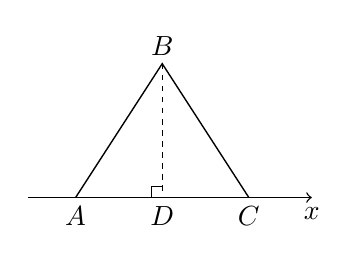
\begin{tikzpicture}[scale=1,line width=0.5pt]
\draw[->] (-0.4,0) -- (3.2,0) node[below] {$x$};
\draw (0.2,0) -- (1.3,1.7) -- (2.4,0);
\node at (0.2,-0.24) {$A$};
\node at (1.3,-0.24) {$D$};
\node at (2.4,-0.24) {$C$};
\node at (1.3,1.92) {$B$};
\draw[dash pattern=on 2pt off 2pt] (1.3,1.7) -- (1.3,0);
\draw (1.16,0) -- (1.16,0.14) -- (1.3,0.14);
\end{tikzpicture}
\end{center}
\step{$AB=AC=BC=\dfrac{2\sqrt3}3$，则 $x_2=x_1+AD=x_1+\dfrac{\sqrt3}3$，$x_3=x_1+\dfrac{2\sqrt3}3$，}
\step{存在 $x_1=-\dfrac{\sqrt3}3$，使得 $x_2=x_1+\dfrac{\sqrt3}3=0\in\Q$，且 $x_3=x_1+\dfrac{2\sqrt3}3=\dfrac{\sqrt3}3$ 为无理数，}
\step{即 $D(x_2)=1$，$D(x_3)=0$ 与图形一致，符合题意，}
\step{此时，$S_{\triangle ABC}=\dfrac12AC\cdot BD=\dfrac{\sqrt3}3$.}
\step{综上所述，存在这样的点 $A$、$B$、$C$，该正三角形的面积为 $\dfrac{\sqrt3}3$.}
\solend

\fi

\item 已知函数 $f(x)$ 满足：对 $\forall x\in R$，都有 $f(x+2025)\leqslant f(x)+2026$，
$f(x+2026)\geqslant f(x)+2027$，若 $f(1)=0$，则 $f(2)$ 的取值范围是\blankline[4.4em].

\ifanswer
\solbegin
\step{对 $\forall x\in R$，都有 $f(x+2025)\leqslant f(x)+2026$，$f(x+2026)\geqslant f(x)+2027$，}
\step{则 $f(x)+2027\leqslant f(x+2026)=f(x+1+2025)\leqslant f(x+1)+2026$，}
\step{即 $f(x)+1\leqslant f(x+1)$，所以 $f(2)\geqslant f(1)+1=1$；}
\step{$f(x)+2026\geqslant f(x+2025)=f(x+2024+1)\geqslant f(x+2024)+1$}
\step{$\geqslant\cdots\geqslant f(x+1)+2024$，所以 $f(x)+2\geqslant f(x+1)$，}
\step{所以 $f(2)\leqslant f(1)+2=2$；}
\step{即 $f(2)$ 的取值范围是 $[1,2]$.}
\solend

\fi

\end{enumerate}

\bigsec{二、选择题}

\begin{enumerate}
\setcounter{enumi}{12}

\item 若实数 $0<m<n<1$，而实数 $x>1$，则下列不等式正确的是\mbox{（\quad）}

\keepwithprev
A. $m^x<n^x$\qquad\qquad B. $x^m>x^n$\qquad\qquad C. $\log_xm>\log_xn$\qquad D. $\log_mx<\log_nx$

\ifanswer
\solbegin
\step{对于 $A$，函数 $f(t)=t^x$ 是以 $t$ 为变量，$x$ 为常量的幂函数，}
\step{由于 $x>1$，易得 $f(t)$ 在 $(0,+\infty)$ 上严格增，}
\step{$0<m<n<1$，$x>1$，可以得到 $m^x<n^x$，故 $A$ 正确；}
\step{对于 $B$，函数 $g(s)=x^s$，是以 $s$ 为变量，$x$ 为常量的指数函数，}
\step{由于 $x>1$，则 $g(s)$ 严格增，$0<m<n<1$，可以得到 $x^m<x^n$，故 $B$ 不正确；}
\step{对于 $C$，$\log_xm=\dfrac{\lg m}{\lg x}$，$\log_xn=\dfrac{\lg n}{\lg x}$，由于 $0<m<n<1$，则 $\lg m<\lg n<0$，}
\step{$x>1$，则 $\lg x>0$，则有 $\dfrac{\lg m}{\lg x}<\dfrac{\lg n}{\lg x}$，即 $\log_xm<\log_xn$，故 $C$ 不正确；}
\step{对于 $D$，由 $\log_mx-\log_nx=\dfrac{\lg x}{\lg m}-\dfrac{\lg x}{\lg n}=\dfrac{\lg x(\lg n-\lg m)}{\lg m\lg n}$，}
\step{因为实数 $0<m<n<1$，而实数 $x>1$，}
\step{所以 $\lg x>0$，$\lg m<\lg n<0$，则 $\dfrac{\lg x(\lg n-\lg m)}{\lg m\lg n}>0$，即 $\log_mx>\log_nx$，}
\step{故 $D$ 不正确.}
\step{故选 $A$.}
\solend

\fi

\item 已知 $x>1$，$y>1$，则 “$4^x>2^y$” 是 $\log_2x>\log_4(y-1)$ ”的\mbox{（\quad）}

\keepwithprev
A. 充分不必要条件\qquad\qquad B. 必要不充分条件

C. 充要条件\qquad\qquad D. 既不充分也不必要条件

\ifanswer
\solbegin
\step{因为 $x>1$，$y>1$，若 $4^x>2^y$，即 $2^{2x}>2^y$，所以 $2x>y>1$，}
\step{因为 $\dfrac y2-\sqrt{y-1}=\dfrac{(\sqrt{y-1})^2-2\sqrt{y-1}+1}2=\dfrac{(\sqrt{y-1}-1)^2}2\geqslant0$，}
\step{即 $\dfrac y2\geqslant\sqrt{y-1}>0$，所以 $\log_2\dfrac y2\geqslant\log_2\sqrt{y-1}=\dfrac12\log_2(y-1)=\log_4(y-1)$，}
\step{又 $x>\dfrac y2>\dfrac12$，所以 $\log_2x>\log_2\dfrac y2\geqslant\log_4(y-1)$，故充分性成立；}
\step{取 $x=2$，$y=4$，满足 $1=\log_2x>\log_4(y-1)=\log_43$，}
\step{但 $16=4^x=2^y=16$，即不满足 $4^x>2^y$，故必要性不成立.}% 链首链尾两个 16 系原卷笔误，应为 4^x=2^y=16，照录
\step{故选 $A$.}
\solend

\fi

\item 以下命题中，真命题的个数是\mbox{（\quad）}

①函数 $y=(x^2+1)^2+3$ 最小值为 3；②若 $2^a+\log_2a=4^b+2\log_4b$，则 $a<2b$；③不等式
$2^x-x-1>0$ 的解集为 $(1,+\infty)$.

\keepwithprev
A. $0$\qquad\qquad B. $1$\qquad\qquad C. $2$\qquad\qquad D. $3$

\ifanswer
\solbegin
\step{对于①，由于 $x^2+1\geqslant1$，则 $y=(x^2+1)^2+3\geqslant4$，}
\step{即函数 $y=(x^2+1)^2+3$ 最小值为 4，①错误；}
\step{对于②，由于 $b>0$，}
\step{则有 $2^a+\log_2a=4^b+2\log_4b=2^{2b}+\log_2b<2^{2b}+\log_22b$，}
\step{设 $f(x)=2^x+\log_2x$，易得 $f(x)$ 在 $(0,+\infty)$ 上为严格增函数，必有 $a<2b$，}
\step{②正确；}
\step{对于③，当 $x=-1$ 时，$2^x-x-1=2^x(x+1)>0$，即 $-1$ 在不等式的解集内，}
\step{③错误；}
\step{故选 $B$.}
\solend

\fi

\item 已知函数 $f(x)=ax^2+bx+c$（$a\neq0$ 且 $a<b$），若对任意的 $x\in R$，$f(x)\geqslant0$，且
$f(1)\geqslant\lambda(b-a)$，则实数 $\lambda$ 的取值范围为\mbox{（\quad）}

\keepwithprev
A. $(-\infty,2]$\qquad\qquad B. $[2\text{，}+\infty)$\qquad\qquad C. $(-\infty\text{，}3]$\qquad\qquad D. $[3\text{，}+\infty)$% 原卷 B/C/D 用全角逗号、A 用半角，照录

\ifanswer
\solbegin
\step{因为函数 $f(x)\geqslant0$ 恒成立，所以 $a>0$，且 $\Delta=b^2-4ac\leqslant0$，即 $c\geqslant\dfrac{b^2}{4a}$，}
\step{所以 $a+b+c\geqslant a+b+\dfrac{b^2}{4a}$，又 $a<b$，所以 $b-a>0$，}
\step{又 $f(1)\geqslant\lambda(b-a)$ 恒成立，所以 $a+b+c\geqslant\lambda(b-a)$ 恒成立，}
\step{即 $\lambda\leqslant\left(\dfrac{a+b+c}{b-a}\right)_{\min}=\dfrac{a+b+\dfrac{b^2}{4a}}{b-a}$，}
\step{令 $t=\dfrac ba$（$t>1$），则 $\dfrac{a+b+\dfrac{b^2}{4a}}{b-a}=\dfrac{1+t+\dfrac{t^2}4}{t-1}$，}
\step{令 $\mu=t-1$（$\mu>0$），则 $t=\mu+1$，}
\step{故上式 $=\dfrac{1+\mu+1+\dfrac{(\mu+1)^2}4}{\mu}=\dfrac14\left(\mu+\dfrac9\mu+6\right)$，}
\step{对 $\mu>0$，有 $\mu+\dfrac9\mu\geqslant2\sqrt{\mu\times\dfrac9\mu}=6$，当且仅当 $\mu=\dfrac9\mu$，即 $\mu=3$ 时取等号，}
\step{所以 $\dfrac14\left(\mu+\dfrac9\mu+6\right)\geqslant\dfrac14(6+6)=3$，故 $\lambda\leqslant3$，}
\step{即实数 $\lambda$ 的取值范围为 $(-\infty,3]$. 故选 $C$.}
\solend

\fi

\end{enumerate}

\bigsec{三、解答题}

\begin{enumerate}
\setcounter{enumi}{16}

\item 已知函数 $f(x)=\log_\frac23(ax^2-6x+18)$.

（1）若 $f(x)$ 的定义域为 $R$，求实数 $a$ 的取值范围.

（2）若 $f(x)$ 的值域为 $R$，求实数 $a$ 的取值范围.

\ansspace*[10]

\ifanswer
\solbegin
\stepm{（1）}{由 $f(x)=\log_\frac23(ax^2-6x+18)$ 的定义域为 $R$，得 $ax^2-6x+18>0$ 恒成立，}
\step{$a=0$ 时，$f(x)=\log_\frac23(18-6x)$ 的定义域为 $(-\infty,3)$，不符合题意.}
\step{$a\neq0$ 时，$\begin{cases}a>0\\ \Delta=36-4\times18a<0\end{cases}$，解得 $a>\dfrac12$.}
\step{综上，$a$ 的取值范围是 $\left(\dfrac12,+\infty\right)$.}
\stepm{（2）}{$a=0$ 时，$f(x)=\log_\frac23(18-6x)$ 的值域为 $R$，符合题意.}
\step{$a\neq0$ 时，$\begin{cases}a>0\\ \Delta=36-4\times18a\geqslant0\end{cases}$，解得 $0<a\leqslant\dfrac12$.}
\step{综上，$a$ 的取值范围是 $\left[0,\dfrac12\right]$.}
\solend

\fi

\item 已知 $f(x)=\log_ax+\log_a(6-x)$，$a>0$ 且 $a\neq1$，且 $f(3)=2$.

（1）求 $a$ 的值及 $f(x)$ 的单调区间.

（2）若对于 $\forall x_1\in(0,6)$，$\exists x_2\in[1,9]$，使得 $f(x_1)\leqslant t+\log_3x_2$ 成立，求实数 $t$ 的取值范
围.

\ansspace*[12]

\ifanswer
\solbegin
\stepm{（1）}{已知 $f(x)=\log_ax+\log_a(6-x)$，且 $f(3)=2$.}
\step{得 $\log_a3+\log_a(6-3)=2$，即 $2\log_a3=2$，}
\step{因此 $\log_a3=1$，因此 $a=3$，因此 $f(x)=\log_3x+\log_3(6-x)$，}
\step{因为 $\begin{cases}x>0\\ 6-x>0\end{cases}$，因此 $0<x<6$，故 $f(x)$ 的定义域为 $(0,6)$；}
\step{$f(x)=\log_3(6x-x^2)$，}
\step{因为函数 $y=6x-x^2$ 在 $(0,3)$ 上严格增，在 $(3,6)$ 上严格减，}
\step{又函数 $y=\log_3x$ 为严格增函数，}
\step{由复合函数的单调性得函数 $f(x)$ 在 $(0,3)$ 上严格增，在 $(3,6)$ 上严格减；}
\stepm{（2）}{令 $g(x)=t+\log_3x$，}
\step{因为 $\forall x_1\in(0,6)$，$\exists x_2\in[1,9]$，使得 $f(x_1)\leqslant t+\log_3x_2$，}
\step{即 $f(x_{1})_{\max}\leqslant g(x_{2})_{\max}$，}
\step{其中由（1）得 $f(x_{1})_{\max}=f(3)=2$.}
\step{又 $g(x)=t+\log_3x$ 在 $[1,9]$ 上严格增，因此 $g(x)_{\max}=g(9)=t+2$，}
\step{因此 $2\leqslant t+2$，因此实数 $t$ 的取值范围为 $[0,+\infty)$.}
\solend

\fi

\item 某心理学研究小组在对学生上课注意力集中情况的调查研究中，发现其注意力指数 $p$ 与
听课时间 $t$ 之间的关系满足如图所示的曲线. 当 $t\in(0,14]$ 时，曲线是二次函数图象的一部
分，当 $t\in[14,40]$ 时，曲线是函数 $y=\log_a(t-5)+83$（$a>0$ 且 $a\neq1$）图象的一部分. 根据
专家研究，当注意力指数 $p$ 大于等于 80 时听课效果最佳.

（1）试求 $p=f(t)$ 的函数关系式；

（2）当一位学生在坚持听课 32 分钟时，注意力指数 $p$ 大约为多少？

（3）一道数学难题，讲解需要 20 分钟，问老师能否经过合理安排在学生听
课效果最佳时讲完？请说明理由.

\begin{center}
% 原图第 9 页题干 p-t 曲线图按原图形状用 TikZ 重排（三版都出）。
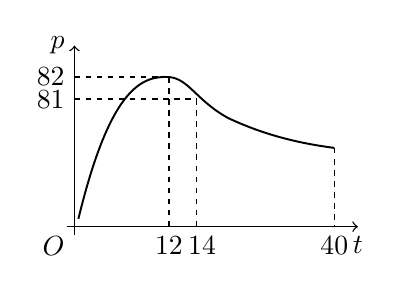
\begin{tikzpicture}[scale=1,line width=0.5pt]
\draw[->] (-0.1,0) -- (3.6,0) node[below] {$t$};
\draw[->] (0,-0.1) -- (0,2.3) node[left] {$p$};
\node[below left] at (0,0) {$O$};
\draw[line width=0.7pt] (0.05,0.1) .. controls (0.45,1.75) and (0.85,1.92) .. (1.2,1.9)
  .. controls (1.45,1.88) and (1.55,1.6) .. (1.95,1.38)
  .. controls (2.5,1.12) and (3.0,1.04) .. (3.3,1.0);
\draw[dash pattern=on 2pt off 2pt] (0,1.9) -- (1.2,1.9);
\draw[dash pattern=on 2pt off 2pt] (0,1.62) -- (1.55,1.62);
\draw[dash pattern=on 2pt off 2pt] (1.2,1.9) -- (1.2,0);
\draw[dash pattern=on 2pt off 2pt] (1.55,1.62) -- (1.55,0);
\draw[dash pattern=on 2pt off 2pt] (3.3,1.0) -- (3.3,0);
\node[left] at (0,1.9) {$82$};
\node[left] at (0,1.62) {$81$};
\node[below] at (1.2,0) {$12$};
\node[below] at (1.62,0) {$14$};
\node[below] at (3.3,0) {$40$};
\end{tikzpicture}
\end{center}

\ansspace*[12]

\ifanswer
\solbegin
\stepm{（1）}{由题意得当 $t\in(0,14]$ 时，设 $f(t)=c(t-12)^2+82$（$c<0$），}
\step{又 $f(14)=81$，所以 $c(14-12)^2+82=81$，解得 $c=-\dfrac14$；}
\step{所以 $f(t)=-\dfrac14(t-12)^2+82$,$t\in(0,14]$；}
\step{又当 $t\in[14,40]$ 时，函数 $y=\log_a(t-5)+83$（$a>0$ 且 $a\neq1$），}
\step{又当 $x=14$ 时，$y=81$，所以 $81=\log_a(14-5)+83$，解得 $a=\dfrac13$；}
\step{所以 $f(t)=\log_\frac13(t-5)+83$,$t\in[14,40]$，}
\step{所以 $p=\begin{cases}-\dfrac14(t-12)^2+82, & t\in(0,14]\\ \log_\frac13(t-5)+83, & t\in(14,40]\end{cases}$；}
\stepm{（2）}{当 $t=32$ 时，$p=\log_\frac13(32-5)+83=80$，}
\step{所以当一位学生在坚持听课 32 分钟时，注意力指数 $p$ 大约为 80；}
\stepm{（3）}{当 $t\in(0,14]$ 时，$-\dfrac14(t-12)^2+82\geqslant80$，解得 $t\in[12-2\sqrt2,14]$，}
\step{当 $t\in[14,40]$ 时，$\log_\frac13(t-5)+83\geqslant80$，解得 $5<t\leqslant32$，则 $t\in[14,32]$，}
\step{因此当 $t\in[12-2\sqrt2,32]$ 时学生听课效果最佳，}
\step{此时 $\Delta t=32-(12-2\sqrt2)=20+2\sqrt2>20$，}
\step{所以老师能经过合理安排时间在学生听课效果最佳时段讲完.}
\solend

\fi

\item 已知 $a\in R$，函数 $f(x+1)=\log_2\left(\dfrac{ax+1+a}{x+1}\right)$.

（1）若 $a=2$，求函数 $f(x)$ 的表达式及定义域；

（2）若关于 $x$ 的方程 $f\left(\dfrac x2\right)-\log_2[(a-2)x+3a-5]=0$ 的解集中恰好只有一个元素，求实
数 $a$ 的取值范围.

\ansspace*[14]

\ifanswer
\solbegin
\stepm{（1）}{$f(x+1)=\log_2\left(\dfrac{ax+1+a}{x+1}\right)$，}
\step{令 $x+1=t$，则 $f(t)=\log_2\left(\dfrac1t+a\right)$，即 $f(x)=\log_2\left(\dfrac1x+a\right)$，}
\step{因为 $a=2$，所以 $f(x)=\log_2\left(2+\dfrac1x\right)$，}
\step{由 $2+\dfrac1x>0$ 得定义域为 $\left(-\infty,-\dfrac12\right)\cup(0,+\infty)$；}
\stepm{（2）}{由（1）得 $f(x)=\log_2\left(\dfrac1x+a\right)$，}
\step{方程 $f\left(\dfrac x2\right)-\log_2[(a-2)x+3a-5]=0$，}
\step{即 $\log_2\left(\dfrac2x+a\right)-\log_2[(a-2)x+3a-5]=0$，}
\step{可转化为 $(a-2)x^2+(2a-5)x-2=0$，且 $\dfrac2x+a>0$.}
\step{①当 $a-2=0$，即 $a=2$ 时，$x=-2$，符合题意；}
\step{②当 $a-2\neq0$，即 $a\neq2$ 时，$x_1=-2$,$x_2=\dfrac1{a-2}$，}
\step{（$i$）当 $-2=\dfrac1{a-2}$ 时，即 $a=\dfrac32$ 时，符合题意；}
\step{（$ii$）当 $-2\neq\dfrac1{a-2}$ 时，即 $a\neq\dfrac32$ 且 $a\neq2$ 时，}
\step{要满足题意，则有 $\begin{cases}-1+a>0\\ 3a-4\leqslant0\end{cases}\Rightarrow1<a\leqslant\dfrac43$ 或 $\begin{cases}-1+a\leqslant0\\ 3a-4>0\end{cases}$，无解；}
\step{综上，$a$ 的取值范围 $\left(1,\dfrac43\right]\cup\left\{2,\dfrac32\right\}$.}
\solend

\fi

\item 已知函数 $y=f(x)$ 是定义在 $[0,+\infty)$ 上的函数，并且 $f(x)\geqslant0$，对于定义域内的任意自
变量的值 $x$、$y$，满足 $f(y)f(x^2f(y)+xf(y))=f(x^2+y+x)$，$f(a)=0$，其中
$a>0$.

（1）当 $f(0)\neq0$ 时，求 $f(0)$；

（2）已知当 $0\leqslant x<a$ 时，有 $f(x)\neq0$.

（$i$）求 $f(a+3)$；

（$ii$）求函数 $y=f(x)$ 的解析式（用 $a$ 表示）.

\ansspace*[16]

\ifanswer
\solbegin
\stepm{（1）}{因为 $f(x)\geqslant0$，且对于定义域内的任意自变量的值 $x$、$y$，}
\step{满足 $f(y)f(x^2f(y)+xf(y))=f(x^2+y+x)$，}
\step{令 $x=y=0$，则 $f^2(0)=f(0)$，因为 $f(0)\neq0$，所以 $f(0)=1$，}
\stepm{（2）}{（$i$）由 $f(y)f(x^2f(y)+xf(y))=f(x^2+y+x)$，}
\step{得 $f(y)f[(x^2+x)f(y)]=f[(x^2+x)+y]$，}
\step{令 $t=x^2+x$，因为 $x\geqslant0$，所以 $t=x^2+x\in[0,+\infty)$，}
\step{所以有 $f(y)f(tf(y))=f(t+y)$，因为 $f(a)=0$，}
\step{令 $y=a$，$t=3$，得 $f(a+3)=f(a)f(3f(a))=0\times f(3f(a))=0$；}
\step{（$ii$）当 $x\geqslant a$ 时，令 $y=a$，$t=x-a$，}
\step{$f(x)=f(x-a+a)=f(a)f[(x-a)f(a)]=0$.}
\step{当 $0\leqslant x<a$ 时，则有 $0<a-x\leqslant a$，令 $y=x$，$t=a-x$，}
\step{则 $f(a)=f(a-x+x)=f(x)f[(a-x)f(x)]=0$.}
\step{因为 $f(x)\neq0$，所以有 $f((a-x)f(x))=0$，则 $(a-x)f(x)\geqslant a$，}
\step{又因为 $a-x>0$，即 $f(x)\geqslant\dfrac a{a-x}$.}
\step{令 $t=\dfrac a{f(x)}>0$,$y=x>0$，}
\step{则 $f\left(\dfrac a{f(x)}+x\right)=f(x)\cdot f\left(\dfrac a{f(x)}\cdot f(x)\right)=f(x)\cdot f(a)=0$，}
\step{所以有 $\dfrac a{f(x)}+x\geqslant a$，即 $\dfrac a{f(x)}\geqslant a-x$，得 $f(x)\leqslant\dfrac a{a-x}$，}
\step{所以当 $0\leqslant x<a$ 时，$f(x)=\dfrac a{a-x}$.}
\step{综上，$f(x)=\begin{cases}\dfrac a{a-x}, & 0\leqslant x<a\\ 0, & x\geqslant a\end{cases}$.}
\solend

\fi

\end{enumerate}

\end{document}
